% -*- LaTeX -*-
% ----------------------------------------------------------------------
%
% Brad T. Aagaard, U.S. Geological Survey
% Charles A. Williams, GNS Science
% Matthew G. Knepley, University of Chicago
%
% This code was developed as part of the Computational Infrastructure
% for Geodynamics (http://geodynamics.org).
%
% Copyright (c) 2010-2019 University of California, Davis
%
% See LICENSE.md for license information.
%
% ----------------------------------------------------------------------
\documentclass{pylithdoc}

\usepackage{graphicx}
\usepackage{array}
\usepackage{multirow} % tables
\usepackage{mathtools} % equations
\usepackage{bm} % equations (bold math)
\usepackage{siunitx} % units

% Units
% \si{\meter\per\second}
%
% Tables
% \begin{table}
% \caption{}
% \label{tab:}
% \begin{tabular}{}
% \toprule
% \thead{}
% \midrule
% \bottomrule
% \end{tabular}
% \end{table}

% ----------------------------------------------------------------------
% Markup
% ----------------------------------------------------------------------
\newcommand{\brad}[1]{{\color{red}{\bf BRAD}: #1}}
\newcommand{\matt}[1]{{\color{blue}{\bf MATT}: #1}}
\newcommand{\charles}[1]{{\color{green}{\bf CHARLES}: #1}}

% ----------------------------------------------------------------------
% Equation macros
% ----------------------------------------------------------------------
\newcommand{\trialvec}[1][]{{\vec{\psi}_\mathit{trial}^{#1}}}
\newcommand{\trialscalar}[1][]{{\psi_\mathit{trial}^{#1}}}
\newcommand{\basisvec}[1][]{{\vec{\psi}_\mathit{basis}^{#1}}}
\newcommand{\basisscalar}[1][]{{\psi_\mathit{basis}^{#1}}}

\newcommand{\tensor}[1]{\bm{#1}}
\DeclareMathOperator{\Tr}{Tr}

\newcommand{\eqnannotate}[2]{%
  {\color{blue}%
  \underbrace{\color{black}#1}_{\color{blue}\mathclap{#2}}}}


%\newcommand{\yes}{\ding{52}}
%\newcommand{\rlabel}[1]{\rotatebox[origin=l]{90}{#1}}


% ----------------------------------------------------------------------
% Version
% ----------------------------------------------------------------------
\renewcommand{\pylithVersionNumber}{3.0.0dev}
\renewcommand{\pylithDOI}{10.5281/zenodo.XXXXXX}
% Update install/install.tex (version number within verbatim environment)

\title{PyLith User Manual}
\author{\copyright University of California, Davis\\ Version \pylithVersionNumber}
\date{\today}

\begin{document}

% -*- LaTeX -*-
%
% ----------------------------------------------------------------------
%
% Brad T. Aagaard, U.S. Geological Survey
% Charles A. Williams, GNS Science
% Matthew G. Knepley, University of Chicago
%
% This code was developed as part of the Computational Infrastructure
% for Geodynamics (http://geodynamics.org).
%
% Copyright (c) 2010-2017 University of California, Davis
%
% See LICENSE.md for license information.
%
% ----------------------------------------------------------------------
%

\newcommand{\HRule}{\rule{\textwidth}{0.2em}}
\noindent\MakeUppercase{{\sffamily\Large Computational Infrastructure for Geodynamics (CIG)}}\\
\HRule
\vspace{2em}

\noindent\begin{tikzpicture}
  \node[draw=none,
  inner sep=1.0em,
  fill=mdblue,
  minimum width=0.3333\textwidth,
  scale=3.0,
]{\color{white}\Huge PyLith};
\end{tikzpicture}
{\raggedleft{\Huge User Manual}\\[8pt]
  {\LARGE Version \pylithVersionNumber}\\}
{\centering\includegraphics[height=0.5\textheight]{cover/coverimage}\\}
{\raggedleft\LARGE Brad Aagaard \\ Matthew Knepley \\ Charles Williams\\}
\vfill
\noindent{\sffamily\LARGE geodynamics.org}\\
\HRule
\thispagestyle{empty}

\maketitle

\frontmatter
\tableofcontents{}
\listoffigures
\listoftables


\chapter{Preface}


\section{About This Document}

This document is organized into two parts. The first part begins with
an introduction to PyLith and discusses the types of problems that
PyLith can solve and how to run the software; the second part provides
appendices and references.


\section{Who Will Use This Documentation}

This documentation is aimed at two categories of users: scientists
who prefer to use prepackaged and specialized analysis tools, and
experienced computational Earth scientists. Of the latter, there are
likely to be two classes of users: those who just run models, and
those who modify the source code. Users who modify the source are
likely to have familiarity with scripting, software installation,
and programming, but are not necessarily professional programmers.

\section{Conventions}

\warning{This is a warning.}
\important{This is something important.}
\tip{This is a tip, helpful hint, or suggestion.}

For features recently added to PyLith, we show the version number when
they were added.\newfeature{v2.1.4}

\subsection{Command Line Arguments}

Exmaple of a command line argument: \commandline{-{}-help}.

\subsection{Filenames and Directories}

Example of filenames and directories: \filename{pylith}, \filename{/usr/local}.

\subsection{Unix Shell Commands}

Commands entered into a Unix shell (i.e., terminal) are shown in a
box. Comments are delimited by the \# character. We use 
{\tt \$\$} to indicate the bash shell prompt.
\begin{shell}
# This is a comment.
$$ ls -l
\end{shell}

\subsection{Excerpts of cfg Files}

Example of an excerpt from a \filename{.cfg} file:
\begin{cfg}
# This is a comment.
<h>[pylithapp.problem]</h>
<p>timestep</p> = 2.0*s ; Time step comment.
<f>bc</f> = [x_pos, x_neg]
\end{cfg}

\section{Citation}

The Computational Infrastructure for Geodynamics (CIG) (\url{geodynamics.org})
is making this source code available to you at no cost in hopes that
the software will enhance your research in geophysics. A number of
individuals have contributed a significant portion of their careers
toward the development of this software. It is essential that you
recognize these individuals in the normal scientific practice by citing
the appropriate peer-reviewed papers and making appropriate acknowledgments
in talks and publications. The preferred way to generate the list
of publications (in Bib\TeX{} format) to cite is to run your simulations
with the \commandline{-{}-include-citations} command line argument, or
equivalently, the \commandline{-{}-petsc.citations} command line argument.
The \commandline{-{}-help-citations} command line argument will generate
the Bib\TeX{} entries for the references mentioned below.

The following peer-reviewed paper discussed the development of PyLith:
\begin{itemize}
\item Aagaard, B. T., M. G. Knepley, and C. A. Williams (2013). A domain
decomposition approach to implementing fault slip in finite-element
models of quasi-static and dynamic crustal deformation, \textit{Journal
of Geophysical Research: Solid Earth}, 118, doi: 10.1002/jgrb.50217.
\end{itemize}
To cite this manual, use:
\begin{itemize}
\item Aagaard, B., M. Knepley, C. Williams (2016), \emph{PyLith User Manual,
Version 2.1.4.} Davis, CA: Computational Infrastructure of Geodynamics.\\
URL: geodynamics.org/cig/software/pylith/pylith\_manual-2.1.4.pdf
\end{itemize}

\section{Support}

Current PyLith development is supported by the CIG, and internal GNS
Science \url{www.gns.cri.nz} and U.S. Geological Survey \url{www.usgs.gov}
funding. Pyre development was funded by the Department of Energy's
\url{www.doe.gov/engine/content.do} Advanced Simulation and Computing
program and the National Science Foundation's Information Technology
Research (ITR) program.

This material is based upon work supported by the National Science
Foundation under Grants No. 0313238, 0745391, and EAR-0949446. Any
opinions, findings, and conclusions or recommendations expressed in
this material are those of the author(s) and do not necessarily reflect
the views of the National Science Foundation.


\section{Acknowledgments}

Many members of the community contribute to PyLith through reporting
bugs, suggesting new features and improvements, running benchmarks,
and asking questions about the software. In particular, we thank Surendra
Somala for contributing to the development of the fault friction implementation.


\section{Request for Comments}

Your suggestions and corrections can only improve this documentation.
Please report any errors, inaccuracies, or typos to the CIG Short-Term
Tectonics email list \url{cig-short@geodynamics.org}. 

\mainmatter\raggedbottom

\chapter{Introduction}

\section{Overview}

PyLith is a multi-scale simulation software package for earthquake
physics. It is portable, scalable software for simulation of crustal
deformation across spatial scales ranging from meters to hundreds of
kilometers and temporal scales ranging from milliseconds to thousands
of years

\section{History}

This first version of PyLith is a direct descendant of Lithomop and
marks the first version that runs in parallel. Lithomop was the
product of major reengineering of Tecton, a finite-element code for
simulating static and quasi-static crustal deformation. The major new
features present in Lithomop included dynamic memory allocation and
the use of the Pyre simulation framework and PETSc solvers. </para>
<para> PyLith is currently being rewritten from scratch to create a
much more modular, powerful simulation package. This new code will
include earthquake dynamics (both rupture propagation and seismic wave
propagation). A beta release is expected in late 2006.

\section{Governing Equations}

Both LithoMop3d and PyLith-0.8 are quasi-static codes, meaning that
time-dependence only enters through the constitutive relationships and
the loading conditions. The description here is for the small-strain
formulation, which is the only formulation available at present. If a
large deformation solution is desired, interested users may contact
Charles Williams (willic3@rpi.edu) about a version of the finite
element code TECTON.

The problem is formulated in terms of the stresses ($\sigma_{ij}$),
displacements ($u_i$), and body forces per unit volume
(figs/g-inlineeq1.eps). We use standard index notation for all
equations here, such that repeated indices imply summation and a comma
denotes differentiation. For a general three-dimensional body, the
problem must satisfy the equilibrium conditions
\begin{equation}
  \text{figs/g-eq1.eps}
\end{equation}
subject to the natural boundary conditions
\begin{equation}
  \text{figs/g-eq2.eps}
\end{equation}
and the essential boundary conditions
\begin{equation}
  \text{figs/g-eq3.eps}
\end{equation}
The surface of the body is $S$, given by
\begin{equation}
  \text{figs/g-eq4.eps}
\end{equation}
The $n_j$ are the components of the unit normal vector to $S$, the
\begin{equation}
  \text{figs/g-inlineeq2.eps}
\end{equation}
are the components of the surface tractions, and the 
\begin{equation}
  \text{figs/g-inlineeq3.eps}
\end{equation}
are the components of the applied displacements. The stresses are
computed from the strains and any existing initial stresses using a
given constitutive relationship. The strains are given by
\begin{equation}
\text{figs/g-eq5.eps}  
\end{equation}
For a linear elastic material, the constitutive relationship between
stress and strain is
\begin{equation}
  \text{figs/g-eq6.eps}
\end{equation}
where
\begin{equation}
  \text{figs/g-inlineeq4.eps}
\end{equation}
are the initial stresses, and $C$
\begin{equation}
  \text{g-inlineeq5.eps}
\end{equation}
is the elastic constitutive relation.

For inelastic behavior (viscous, plastic, etc.), we assume an additive
decomposition of the strain tensor into elastic and inelastic parts,
and use an integrated form of the classical incremental theory of
plasticity. At time $t+\Delta t$, he stresses are therefore computed
from the total elastic strain:
\begin{equation}
  \text{figs/g-eq7.eps}
\end{equation}
where
\begin{equation}
  \text{figs/g-inlineeq6.eps}
\end{equation}
are the total strains and
\begin{equation}
  \text{figs/g-inlineeq7.eps}
\end{equation}
are the inelastic strains, with the difference being the elastic
strains. In our actual computations, we use a formulation that
decomposes the stresses into the deviatoric and volumetric parts,
using ideas based on the "effective stress function"
\cite{Kojic:Bathe:1987}. This allows the time integration of stresses
to be performed in terms of a single parameter related to the second
deviatoric stress invariant.

\section{Software Components}

PyLith is separated into modules to encapsulate behavior and
facilitate use across multiple applications. That way expert users can
replace functionality of a wide variety of components without
recompiling or polluting the main code. External packages reduce
development time and enhance computational efficiency, for example,
PyLith runs 2x faster by using the PETSc linear solver.

PyLith is based on several programming languages. High-level code is
written in Python; this rich, expressive interpreted language with
dynamic typing reduces development time. Low-level code is written in
Fortran 77 for fast execution. Bindings, written in C/C++, are used to
allow the low-level code (Fortran 77) to be called from high-level
code (Python).

PyLith makes extensive use of external software. Pyre is a science
neutral simulation framework being developed at Caltech. PETSc is used
to perform operations on matrices and vectors in parallel.

\subsection{PETSc}

\href{http://www-unix.mcs.anl.gov/petsc/petsc-as/}{PETSc}, the
Portable, Extensible Toolkit for Scientific computation, provides a
suite of routines for parallel, numerical solution of partial
differential equations for linear and nonlinear systems with large,
sparse systems of equations. PETSc includes solvers that implement a
variety of Newton and Krylov subspace methods. It can also interface
with many external packages, including BlockSolve95, ESSL, Matlab,
ParMeTis, PVODE, and SPAI, thereby providing additional solvers and
interaction with other software packages.

PETSc includes interfaces for Fortran, C, and C++ for nearly all of
the routines and PETSc can be installed on most Unix systems. PETSc
can be built with user supplied highly optimized linear algebra
routines (e.g., ATLAS and commercial versions of BLAS/LAPACK), thereby
improving application performance. Users can use PETSc parallel
matrices, vectors, and other data structures for most parallel
operations, eliminating the need for explicit calls to Message Passing
Interface (MPI) routines. Many settings and options can be controlled
with PETSc specific command-line arguments, including selection of
preconditions, solvers, and generation of performance logs.

\subsection{Pyre}

Pyre is an object-oriented environment capable of specifying and
launching numerical simulations on multiple platforms, including
Beowulf class parallel computers and grid computing systems. Pyre
allows the binding of multiple components such as solid and fluid
models used in Earth science simulations, and different meshers. The
Pyre framework enables the elegant setup, modification and launching
of massively parallel three-dimensional solver applications.

Pyre is a framework, a combination of software and design philosophy
that promotes the reuse of code. In their canonical software design
book, {\em Design Patterns}, Erich Gamma {\it et al}.  condense the
concept of a framework concept down to, "When you use a framework, you
reuse the main body and write the code it calls." In the context of
frameworks and object-oriented programming, Pyre can be thought of as
a collection of classes and the way their instances interact.
Programming applications based on Pyre will look similar to those
written in any other object-oriented language. The Pyre framework
contains a subset of parts that make up the overall framework. Each of
those parts is designed to solve a specific problem.

The framework approach to computation offers many advantages. It
permits the exchange of codes and promotes the reuse of standardized
software while preserving efficiency. Frameworks are also an efficient
way to handle changes in computer architecture. They present
programmers and scientists with a unified and well-defined task and
allow for shared costs of the housekeeping aspects of software
development. They provide greater institutional continuity to model
development than piecemeal approaches.


The Pyre framework incorporates features aimed at enabling the
scientific non-expert to perform tasks easily without hindering the
expert. Target features for end users allow complete and intuitive
simulation specification, reasonable defaults, consistency checks of
input, good diagnostics, easy access to remote facilities, and status
monitoring. Target features for developers include easy access to user
input, a shorter development cycle, and good debugging support.

\begin{figure}[htbp]
  \begin{center}
    \includegraphics[scale=0.75]{figs/pyre_overview}
    \caption{Pyre Architecture. The integration framework is a set of
      cooperating abstract services.}
  \end{center}
\end{figure}

\section{PyLith Design}

In transforming Lithomop, a serial code, into PyLith, a parallel code,
a principal concern was to preserve the existing structure of the
serial Fortran code. Active development of purely analytic features in
PyLith, such as new material models or discretization schemes, depends
on the familiarity of application scientists with the traditional
Fortran programming paradigm. Global, topological operation should be
strictly segregated from the existing code. In fact, with the
exception of integrating PETSc for serial linear algebra and solver
operations, PyLith can be run purely in serial without activating any
of the parallel capabilities.

In order to accomplish this separation, we use the PETSc
\classname{Sieve} structure to create a model of the serial
PyLith mesh. This model is then partitioned and distributed to a set
of processes. Each process receives a self-consistent mesh, meaning
the pieces are overlapping. Each process then executes a serial PyLith
step on that particular mesh piece. The PETSc linear algebra
operations are overloaded, using the \classname{Sieve}
information, to produce a globally consistent field.



\chapter{\label{cha:Installation-and-Getting}Installation and Getting Help}

Installation of PyLith on a desktop or laptop machine is, in most
cases, very easy. Binary packages have been created for Linux and
Mac OS X platforms. You can also run PyLith inside a Docker container,
which provides a virtual Linux environment on any platform that Docker
supports, including Linux, Mac OS X, and Windows. Installation of
PyLith on other operating systems -- or installation on a cluster
-- requires building the software from the source code, which can
be difficult for inexperienced users. We have created a small utility
called PyLith Installer that makes installing PyLith and all of its
dependencies from source much easier. Help is available from both
a CIG mailing list and the Github issue tracking system \url{https://github.com/geodynamics/pylith/issues}.


\section{\label{sec:Getting-Help-and}Getting Help and Reporting Bugs}

The CIG Short-Term Crustal Dynamics Mailing List \url{cig-short@geodynamics.org}
is dedicated to CIG issues associated with short-term crustal dynamics,
including the use of PyLith. You can subscribe to the mailing list
and view messages at cig-short Mailing List \url{geodynamics.org/cig/lists/cig-short}. 

CIG uses \texttt{Github} for source control and bug tracking. If you
find a bug in PyLith, please submit a bug report to the Github issue
tracking system for PyLith \url{https://github.com/geodynamics/pylith/issues}.
Of course, it is helpful to first check to see if someone else already
submitted a report related to the issue; one of the CIG developers
may have posted a work around to the problem. You can reply to a current
issue by clicking on the issue title. To submit a new issue, click
on the \textsf{New Issue} button.


\section{Installation of Binary Executable}

Binary executables are available for Linux and Mac OS X (Intel 10.10+)
from the PyLith web page \url{geodynamics.org/cig/software/packages/short/pylith/}.


\subsection{Linux}
\begin{enumerate}
\item Open a terminal window and change to the directory where you want
to place the distribution.

\begin{lyxcode}
\$~cd~\$HOME

\$~mkdir~pylith

\$~cd~pylith
\end{lyxcode}
\item Download the Linux tarball from the PyLith web page \url{geodynamics.org/cig/software/packages/short/pylith/},
and save it to the desired location, e.g., \texttt{\$HOME/pylith}.
\item Unpack the tarball.

\begin{lyxcode}
\$~tar~-xzf~pylith-2.1.4-linux-i686.tgz
\end{lyxcode}
\item Set environment variables. The provided \texttt{setup.sh} script only
works if you are using bash shell. If you are using a different shell,
you will need to alter how the environment variables are set in \texttt{setup.sh}.

\begin{lyxcode}
\$~source~setup.sh
\end{lyxcode}
\end{enumerate}

\subsection{Mac OS X}
\begin{enumerate}
\item Open a terminal window and change to the directory where you want
to place the distribution.

\begin{lyxcode}
\$~cd~\$HOME

\$~mkdir~pylith

\$~cd~pylith
\end{lyxcode}
\item Download the Darwin tarball from the PyLith web page \url{geodynamics.org/cig/software/packages/short/pylith/}
and save it to the desired location, e.g., \texttt{\$HOME/pylith}.
\item Unpack the tarball. 

\begin{lyxcode}
\$~tar~-xzf~pylith-2.1.4-darwin-10.11.6.tgz
\end{lyxcode}
\item Set environment variables. The provided \texttt{setup.sh} script only
works if you are using bash shell. If you are using a different shell,
you will need to alter how the environment variables are set in \texttt{setup.sh}.

\begin{lyxcode}
\$~source~setup.sh
\end{lyxcode}
\end{enumerate}

\section{Installation of PyLith Docker Container}

Docker containers provide a self-contained virtual environment that
are a smaller, simpler alternative to a virtual machine. The PyLith
Docker container provides a Debian Linux environment with a pre-built
PyLith executable. These instructions are also available on the PyLith
wiki (\url{https://wiki.geodynamics.org/software:pylith:docker}).


\subsection{Setup (first time only)}
\begin{enumerate}
\item Install Docker (See \url{https://www.docker.com/products/docker})
\item Create container to store persistent user data\\
This container, called pylith-data, will hold a directory where all
your user data can be stored for use with PyLith within Docker. The
data can persist for different versions of PyLith; that is, you can
update to a newer version of PyLith and your user data will still
be available. This directory is not directly accessible from your
host computer. However, you can copy files to/from your host filesystem
using \textquotedblleft{}docker cp\textquotedblright{} (see below).\end{enumerate}
\begin{lyxcode}
\$~docker~create~-{}-name~pylith-data~geodynamics/pylith-data
\end{lyxcode}

\subsection{Run Unix shell within Docker to use PyLith.}
\begin{lyxcode}
\$~docker~run~-ti~-{}-volumes-from~pylith-data~geodynamics/pylith\end{lyxcode}
\begin{quote}
\textbf{Hint}: Within the container, you will probably want to copy
the examples from the pylith-VERSION directory to the data directory,
which is the persistent storage.\end{quote}
\begin{lyxcode}
\$~cp~-R~\textasciitilde{}/pylith-VERSION/examples~\textasciitilde{}/data
\end{lyxcode}

\subsubsection{Using Docker containers}
\begin{itemize}
\item To ``pause'' a container: \texttt{Control-p Control-q}
\item To attach to a ``paused'' or ``running'' container.

\begin{itemize}
\item Get the container id\end{itemize}
\begin{lyxcode}
\$~docker~ps\end{lyxcode}
\begin{itemize}
\item Attach to the container\end{itemize}
\begin{lyxcode}
\$~docker~attach~CONTAINER\_ID
\end{lyxcode}
\end{itemize}

\subsection{Copy data to/from persistent storage volume.}

These commands are run on the local host outside the container, not
inside the Docker container.


\subsubsection{Copy data FROM persistent storage volume TO local host}
\begin{lyxcode}
\$~docker~cp~pylith-data:/data/pylith-user/PATH/FILENAME~LOCAL\_PATH
\end{lyxcode}

\subsubsection{Copy data FROM local host TO persistent storage volume}
\begin{lyxcode}
\$~docker~cp~LOCAL\_PATH~pylith-data:/data/pylith-user/PATH/
\end{lyxcode}

\subsection{Docker Quick Reference}
\begin{itemize}
\item List local docker images\end{itemize}
\begin{lyxcode}
\$~docker~images\end{lyxcode}
\begin{itemize}
\item List all docker containers\end{itemize}
\begin{lyxcode}
\$~docker~ps~-a\end{lyxcode}
\begin{itemize}
\item List running docker containers\end{itemize}
\begin{lyxcode}
\$~docker~ps\end{lyxcode}
\begin{itemize}
\item Remove docker container\end{itemize}
\begin{lyxcode}
\$~docker~rm~CONTAINER\_ID\end{lyxcode}
\begin{itemize}
\item Remove docker image\end{itemize}
\begin{lyxcode}
\$~docker~rmi~IMAGE\_ID
\end{lyxcode}

\section{Installation from Source}

PyLith depends on a number of other packages (see Figure \ref{fig:pylith-dependencies}).
This complicates building the software from the source code. In many
cases some of the packages required by PyLith are available as binary
packages. On the one hand, using the binary packages removes the burden
of configuring, building, and installing these packages, but that
can come with its own host of complications if consistent compiler
and configuration settings are not used across all of the packages
on which PyLith depends. This is usually not an issue with Linux distributions,
such as Fedora, Ubuntu, and Debian that have good quality control;
it can be an issue with Darwin package managers, such as Fink, MacPorts,
and Homebrew, where there is limited enforcement of consistency across
packages. Nevertheless, PyLith can be built on most systems provided
the instructions are followed carefully. PyLith is developed and tested
on Linux and Mac OS X.

A small utility, PyLith Installer, removes most of the obstacles in
building PyLith and its dependencies from source. For each package
this utility downloads the source code, configures it, builds it,
and installs it. This insures that the versions of the dependencies
are consistent with PyLith and that the proper configure arguments
are used. The minimum requirements for using the PyLith installer
are a C compiler, \texttt{tar}, and \texttt{wget} or \texttt{curl}.
Detailed instructions for how to install PyLith using the installer
are included in the installer distribution, which is available from
the PyLith web page \url{geodynamics.org/cig/software/packages/short/pylith/}.


\section{Verifying PyLith is Installed Correctly}

The easiest way to verify that PyLith has been installed correctly
is to run one or more of the examples supplied with the binary and
source code. In the binary distribution, the examples are located
in \texttt{src/pylith-2.1.4/examples} while in the source distribution,
they are located in \texttt{pylith-2.1.4/examples}. Chapter \ref{cha:Tutorials}
discusses how to run and visualize the results for the examples. To
run the example discussed in Section \ref{sec:Tutorial-3d-hex8-static}:
\begin{lyxcode}
\$~cd~examples/3d/hex8~\\
\$~pylith~step01.cfg
\end{lyxcode}
If you run PyLith if a directory without any input, you will get the
error message:
\begin{lyxcode}
>\textcompwordmark{}>~\{default\}::~~~\\
-{}-~pyre.inventory(error)~~~\\
-{}-~meshimporter.meshioascii.filename~<-~''~~~\\
-{}-~Filename~for~ASCII~input~mesh~not~specified.~~To~test~PyLith,~run~an~example~as~discussed~in~the~manual.~~~\\
>\textcompwordmark{}>~\{default\}::~~~\\
-{}-~pyre.inventory(error)~~~\\
-{}-~timedependent.homogeneous.elasticisotropic3d.label~<-~''~~~\\
-{}-~Descriptive~label~for~material~not~specified.~~~\\
>\textcompwordmark{}>~\{default\}::~~~\\
-{}-~pyre.inventory(error)~~~\\
-{}-~timedependent.homogeneous.elasticisotropic3d.simpledb.label~<-~''~~~\\
-{}-~Descriptive~label~for~spatial~database~not~specified.~~~\\
>\textcompwordmark{}>~\{default\}::~~~\\
-{}-~pyre.inventory(error)~~~\\
-{}-~timedependent.homogeneous.elasticisotropic3d.simpledb.simpleioascii.filename~<-~''~~~\\
-{}-~Filename~for~spatial~database~not~specified.~pylithapp:~configuration~error(s)~~
\end{lyxcode}
This indicates that a number of default settings must be set in order
to run PyLith, including setting the filename for the finite-element
mesh.


\section{Configuration on a Cluster}

If you are installing PyLith on a cluster with a batch system, you
can configure Pyre such that the \texttt{pylith} command automatically
submits jobs to the batch queue. Pyre contains support for the LSF,
PBS, SGE, and Globus batch systems.

The command to submit a batch job depends upon the particular batch
system used. Further, the command used in a batch script to launch
an MPI program varies from one cluster to the next. This command can
vary between two clusters, even if the clusters use the same batch
system! On some systems, \texttt{mpirun} is invoked directly from
the batch script. On others, a special wrapper is used instead.

Properly configured, Pyre can handle job submissions automatically,
insulating users from the details of the batch system and the site
configuration. This feature has the most value when the system administrator
installs a global Pyre configuration file on the cluster (under \texttt{/etc/pythia-0.8}),
for the benefit of all users and all Pyre-based applications.


\subsection{\label{sub:Launchers-and-Schedulers}Launchers and Schedulers}

If you have used one of the batch systems, you will know that the
batch system requires you to write a script to launch a job. Fortunately,
launching a parallel PyLith job is simplified by Pyre's \texttt{launcher}
and \texttt{scheduler} facilities. Many properties associated with
\texttt{launcher} and \texttt{scheduler} are pertinent to the cluster
you are on, and are best customized in a configuration file. Your
personal PyLith configuration file (\texttt{\textasciitilde{}/.pyre/pylithapp/pylithapp.cfg})
is suitable for this purpose. On a cluster, the ideal setup is to
install a system-wide configuration file under \texttt{/etc/pythia-0.8},
for the benefit of all users.

Pyre's \texttt{scheduler} facility is used to specify the type of
batch system you are using (if any):
\begin{lyxcode}
{[}pylithapp{]}

scheduler~=~lsf
\end{lyxcode}
The valid values for \texttt{scheduler} are \texttt{lsf}, \texttt{pbs},
\texttt{globus}, and \texttt{none}.

Pyre's \texttt{launcher} facility is used to specify which MPI implementation
you are using:
\begin{lyxcode}
{[}pylithapp{]}

launcher~=~mpich
\end{lyxcode}
The valid values for \texttt{launcher} include \texttt{mpich} and
\texttt{lam-mpi}.

You may find the \texttt{dry} option useful while debugging the \texttt{launcher}
and \texttt{scheduler} configuration. To debug the scheduler configuration,
use the \texttt{-{}-scheduler.dry} option:
\begin{lyxcode}
\$~pylith~-{}-scheduler.dry
\end{lyxcode}
This option will cause PyLith to perform a ``dry run,'' dumping the
batch script to the console, instead of actually submitting it for
execution (the output is only meaningful if you're using a batch system).
Likewise, to debug the launcher configuration, use the \texttt{-{}-launcher.dry}
option:
\begin{lyxcode}
\$~pylith~-{}-launcher.dry
\end{lyxcode}
This option will cause PyLith to print the \texttt{mpirun} command,
instead of actually executing it. (If you're using a batch system,
a job will be submitted for execution; when it runs, PyLith will simply
print the \texttt{mpirun} command, and the job will immediately terminate.)


\subsection{Running without a Batch System}

On a cluster without a batch system, you need to explicitly specify
the machines on which the job will run. Supposing the machines on
your cluster are named n001, n002, \ldots{}, etc., but you want to
run the job on machines n001, n003, n004, and n005 (maybe n002 is
down for the moment). To run an example, create a file named \texttt{mymachines.cfg}
which specifies the machines to use:
\begin{lyxcode}
{[}pylithapp.launcher{]}

nodegen~=~n\%03d

nodelist~=~{[}1,3-5{]}
\end{lyxcode}
The \texttt{nodegen} property is a printf-style format string, used
in conjunction with \texttt{nodelist} to generate the list of machine
names. The \texttt{nodelist} property is a comma-separated list of
machine names in square brackets.

Now, invoke the following:
\begin{lyxcode}
\$~pylith~example.cfg~mymachines.cfg
\end{lyxcode}
This strategy gives you the flexibility to create an assortment of
\texttt{.cfg} files (with one \texttt{.cfg} file for each machine
list) which can be easily paired with different parameter files.

If your machine list does not change often, you may find it more convenient
to specify default values for \texttt{nodegen} and \texttt{nodelist}
in \texttt{\textasciitilde{}/.pyre/pylithapp/pylithapp.cfg} (which
is read automatically). Then, you can run any simulation with no additional
arguments:
\begin{lyxcode}
\$~pylith~example.cfg\end{lyxcode}
\begin{quote}
\textbf{\textcolor{red}{Warning:}}\textbf{ }This assumes your machine
list has enough nodes for the simulation in question.
\end{quote}
You will notice that a machine file \texttt{mpirun.nodes} is generated.
It will contain a list of the nodes where PyLith has run.


\subsection{Using a Batch System}

Many clusters use some implementation of a PBS (e.g., TORQUE/Maui)
or LSF batch system. The examples below illustrate use of some of
the more important settings. You may need to make use of more options
or adjust these to submit jobs on various cluster. These settings
are usually placed in \texttt{\textasciitilde{}/.pyre/pylithapp/pylithapp.cfg}
or in a system-wide configuration file. They can be overridden on
the command line, where one typically specifies the number of compute
nodes and number of processes per compute node, the job name, and
the allotted time for the job:
\begin{lyxcode}
\$~pylith~example1.cfg~-{}-job.queue=debug~\textbackslash{}

~~~~-{}-job.name=example1~-{}-job.stdout=example1.log~-{}-job.stderr=example1.err~\textbackslash{}

~~~~-{}-job.walltime=5{*}minute~\textbackslash{}

~~~~-{}-nodes=4
\end{lyxcode}
Note that the values for nodes is equal to the number of compute nodes
times the number of processes (usually the number of cores) requested
per compute node. Specifying the number of processes per compute node
depends on the batch system. For more information on configuring Pyre
for your batch system, see CIG's Pythia page \url{geodynamics.org/cig/software/packages/cs/pythia}.


\subsubsection{LSF Batch System}
\begin{lyxcode}
{[}pylithapp{]}

scheduler~=~lsf~~~~;~the~type~of~batch~system



{[}pylithapp.lsf{]}

bsub-options~=~{[}-a~mpich\_gm{]}~~~~;~special~options~for~'bsub'



{[}pylithapp.launcher{]}

command~=~mpirun.lsf~~~~;~'mpirun'~command~to~use~on~our~cluster



{[}pylithapp.job{]}

queue~=~normal~~~~;~default~queue~for~jobs
\end{lyxcode}

\subsubsection{PBS Batch System}
\begin{lyxcode}
{[}pylithapp{]}

scheduler~=~pbs~~~~~;~the~type~of~batch~system



{[}pylithapp.pbs{]}

shell~=~/bin/bash~~~~~;~submit~the~job~using~a~bash~shell~script



\#~Export~all~environment~variables~to~the~batch~job

\#~Send~email~to~johndoe@mydomain.org~when~the~job~begins,~ends,~or~aborts

qsub-options~=~-V~-m~bea~-M~johndoe@mydomain.org



{[}pylithapp.launcher{]}

command~=~mpirun~-np~\$\{nodes\}~-machinefile~\$\{PBS\_NODEFILE\}
\end{lyxcode}
For most PBS batch systems you can specify 4 processes per compute
node via the command line argument \texttt{-{}-scheduler.ppn=4}.

\chapter{Governing Equations}
\label{cha:governing:equations}

We present here a brief derivation of the equations for both quasi-static
and dynamic computations. Since the general equations are the same
(except for the absence of inertial terms in the quasi-static case),
we first derive these equations. We then present solution methods
for each specific case. In all of our derivations, we use the notation
described in Table \vref{tab:notation} for both index
and vector notation.

\begin{table}[htbp]
  \caption{Mathematical notation}
  \label{tab:notation}
  \begin{tabular}{cp{3in}}
    \toprule
    {\bf Symbol} & {\bf Description} \\
    \midrule
    $\vec{a}$ & Vector field a \\
    $\tensor{a}$ & Second order tensor field a \\
    $\vec{u}$ & Displacement vector field \\
    $\vec{{d}}$ & Fault slip vector field \\
    $\vec{f}$ & Body force vector field \\
    $\vec{\tau}$ & Traction vector field \\
    $\tensor{\sigma}$ & Stress tensor field \\
    $\vec{n}$ & Normal vector field \\
    $\rho$ & Mass density scalar field \\
    \bottomrule
  \end{tabular}
\end{table}

\section{Derivation of Elasticity Equation}

\subsection{Vector Notation}

Consider volume $V$ bounded by surface $S$. Applying a Lagrangian
description of the conservation of momentum gives
\begin{equation}
\label{eqn:momentum:vec}
\frac{\partial}{\partial t}\int_{V}\rho\frac{\partial\vec{u}}{\partial t}\, dV=\int_{V}\vec{f}\, dV+\int_{S}\vec{\tau}\, dS.
\end{equation}
The traction vector field is related to the stress tensor through
\begin{equation}
\vec{\tau}=\underline{\sigma}\cdot\vec{n},
\end{equation}
where $\vec{n}$ is the vector normal to $S$. Substituting
into equation \vref{eqn:momentum:vec} yields
\begin{equation}
\frac{\partial}{\partial t}\int_{V}\rho\frac{\partial\vec{u}}{\partial t}\, dV=\int_{V}\vec{f}\, dV+\int_{S}\underline{\sigma}\cdot\vec{n}\, dS.
\end{equation}
Applying the divergence theorem,
\begin{equation}
\int_{V}\nabla\cdot\vec{a}\: dV=\int_{S}\vec{a}\cdot\vec{n}\: dS,
\end{equation}
to the surface integral results in
\begin{equation}
\frac{\partial}{\partial t}\int_{V}\rho\frac{\partial\vec{u}}{\partial t}\, dV=\int_{V}\vec{f}\, dV+\int_{V}\nabla\cdot\underline{\sigma}\, dV,
\end{equation}
which we can rewrite as
\begin{equation}
\int_{V}\left(\rho\frac{\partial^{2}\vec{u}}{\partial t^{2}}-\vec{f}-\nabla\cdot\vec{\sigma}\right)\, dV=\vec{0}.
\end{equation}
Because the volume $V$ is arbitrary, the integrand must be the zero
vector at every location in the volume, so that we end up with
\begin{gather}
\rho\frac{\partial^{2}\vec{u}}{\partial t^{2}}-\vec{f}-\nabla\cdot\vec{\sigma}=\vec{0}\text{ in }V,\\
\underline{\sigma}\cdot\vec{n}=\vec{\tau}\text{ on }S_{\tau}\text{,}\\
\vec{u}=\vec{u^{o}}\text{ on }S_{u},\text{ and}\\
\underbar{R}\cdot(\vec{u^{+}}-\vec{u^{-}})=\vec{d}\text{ on }S_{f}.
\end{gather}
We specify tractions, $\vec{\tau}$, on surface $S_{f}$, displacements,
$\vec{u^{o}}$, on surface $S_{u}$, and slip, $\vec{d}$,
on fault surface $S_{f}$ (we will consider the case of fault constitutive
models in Section \vref{sec:fault}). The rotation matrix $\underline{R}$
transforms vectors from the global coordinate system to the fault
coordinate system. Note that since both $\vec{\tau}$ and
$\vec{u}$ are vector quantities, there can be some spatial
overlap of the surfaces $S_{\tau}$ and $S_{u}$; however, the same degree
of freedom cannot simultaneously have both types of boundary conditions.

\section{Time-Dependent Problem (\facilityshape{formulation})}

This type of problem applies to transient static, quasi-static, and
dynamic simulations. The time-dependent problem adds the
\facility{formulation} facility to the general-problem. The
formulation specifies the time-stepping formulation to integrate the
elasticity equation. PyLith provides several alternative formulations,
each specific to a different type of problem.
\begin{description}
\item[\object{Implicit}] Implicit time stepping for static and
   quasi-static problems with infinitesimal strains. The implicit
   formulation neglects inertial terms (see Section
   \vref{eq:elasticity:integral:quasistatic}).
\item[\object{ImplicitLgDeform}] Implicit time stepping for static
  and quasi-static problems including the effects of rigid body motion
  and small strains.  This formulation requires the use of the
  nonlinear solver, which is selected automatically.
\item[\object{Explicit}] Explicit time stepping for dynamic problems
  with infinitesimal strains and lumped system Jacobian. The cell
  matrices are lumped before assembly, permitting use of a vector for
  the diagonal system Jacobian matrix. The built-in lumped solver is
  selected automatically.
\item[\object{ExplicitLgDeform}] Explicit time stepping for dynamic
  problems including the effects of rigid body motion and small
  strains. The cell matrices are lumped before assembly, permitting
  use of a vector for the diagonal system Jacobian matrix. The
  built-in lumped solver is selected automatically.
\item[\object{ExplicitTri3}] Optimized elasticity formulation for
  linear triangular cells with one point quadrature for dynamic
  problems with infinitesimal strains and lumped system Jacobian. The
  built-in lumped solver is selected automatically.
\item[\object{ExplicitTet4}] Optimized elasticity formulation for
  linear tetrahedral cells with one point quadrature for dynamic
  problems with infinitesimal strains and lumped system Jacobian. The
  built-in lumped solver is selected automatically.
\end{description}
In many quasi-static simulations it is convenient to compute a static
problem with elastic deformation prior to computing a transient response.
Up through PyLith version 1.6 this was hardwired into the Implicit
Forumulation as advancing from time step $t=-\Delta t$ to $t=0$,
and it could not be turned off. PyLith now includes a property, \property{elastic\_prestep}
in the TimeDependent component to turn on/off this behavior (the default
is to retain the previous behavior of computing the elastic deformation).

\warning{Turning off the elastic
prestep calculation means the model only deforms when an {\it increment}
in loading or deformation is applied, because the time-stepping formulation
is implemented using the increment in displacement.}

The \object{TimeDependent} properties and facilities include
\begin{inventory}
  \propertyitem{elastic\_preset}{If true, perform a static calculation with elastic
    behavior before time stepping (default is True).}
  \facilityitem{formulation}{Formulation for solving the partial differential
    equation.}
\end{inventory}
An example of setting the properties and components in a \filename{.cfg} file
is
\begin{cfg}
<h>[pylithapp.timedependent]</h>
<f>formulation</f> = pylith.problems.Implicit ; default
<f>progres_monitor</f> = pylith.problems.ProgressMonitorTime ; default
<p>elastic_preset</p> = True ; default
\end{cfg}
The formulation value can be set to the other formulations in a similar
fashion. 


\subsection{Time-Stepping Formulation}

The explicit and implicit time stepping formulations use a common
set of facilities and properties. The properties and facilities include
\begin{inventory}
\propertyitem{matrix\_type}{Type of PETSc matrix for the system Jacobian (sparse
matrix, default is symmetric, block matrix with a block size of 1).}
\propertyitem{view\_jacobian}{Flag to indicate if system Jacobian (sparse matrix)
should be written to a file (default is false).}
\propertyitem{split\_fields}{Split solution field into a displacement portion
(fields 0..ndim-1) and a Lagrange multiplier portion (field ndim)
to permit application of sophisticated PETSc preconditioners (default
is false).}
\facilityitem{time\_step}{Time step size specification (default is \object{TimeStepUniform} (uniform time step).}
\facilityitem{solver}{Type of solver to use (default is \object{SolverLinear}).}
\facilityitem{output}{Array of output managers for output of the solution (default
is [output]).}
\facilityitem{jacobian\_viewer}{Viewer to dump the system Jacobian (sparse matrix)
to a file for analysis (default is PETSc binary).}
\end{inventory}

An example of setting these parameters in a \filename{.cfg} file is
\begin{cfg}
<h>[pylithapp.timedependent.formulation]</h>
<p>matrix_type</p> = sbaij ; Non-symmetric sparse matrix is 'aij'
<p>view_jacobian</p> = false

# Nonlinear solver is pylith.problems.SolverNonlinear
<f>solver</f> = pylith.problems.SolverLinear
<f>output</f> = [domain, ground_surface]
<f>time_step</f> = pylith.problems.TimeStepUniform
\end{cfg}

\subsection{Numerical Damping in Explicit Time Stepping}

In explicit time-stepping formulations for elasticity, boundary conditions
and fault slip can excite short waveform elastic waves that are not
accurately resolved by the discretization. We use numerical damping
via an artificial viscosity\cite{Knopoff:Ni:2001,Day:Ely:2002} to
reduce these high frequency oscillations. In computing the strains
for the elasticity term in equation \vref{eq:elasticity:integral:dynamic:t},
we use an adjusted displacement rather than the actual displacement,
where 
\begin{equation}
\vec{u}^{adj}(t)=\vec{u}(t)+\eta^{*}\Delta t\vec{\dot{u}}(t),
\end{equation}
$\vec{u}^{adj}(t)$ is the adjusted displacement at time t, $\vec{u}(t)$is
the original displacement at time (t), $\eta^{*}$is the normalized
artificial viscosity, $\Delta t$ is the time step, and $\vec{\dot{u}}(t)$
is the velocity at time $t$. The default value for the normalized
artificial viscosity is 0.1. We have found values in the range 0.1-0.4
sufficiently suppress numerical noise while not excessively reducing
the peak velocity. An example of setting the normalized artificial
viscosity in a \filename{.cfg} file is
\begin{cfg}
<h>[pylithapp.timedependent.formulation]</h>
<p>norm_viscosity</p> = 0.2
\end{cfg}

\subsection{Solvers}
\label{sec:solvers}

PyLith supports three types of solvers. The linear solver,
SolverLinear, corresponds to the PETSc KSP solver and is used in
linear problems with linear elastic and viscoelastic bulk constitutive
models and kinematic fault ruptures. The nonlinear solver,
SolverNonlinear, corresponds to the PETSc SNES solver and is used in
nonlinear problems with nonlinear viscoelastic or elastoplastic bulk
constitutive models, dynamic fault ruptures, or problems involving
finite strain (small strain formulation).  The lumped solver
(SolverLumped) is a specialized solver used with the lumped system
Jacobian matrix. The options for the PETSc KSP and SNES solvers are
set via the top-level PETSc options (see Section
\vref{sec:petsc:options} and the PETSc documentation
\url{www.mcs.anl.gov/petsc/petsc-as/documentation/index.html}).


\subsection{Time Stepping}
\label{sub:Time-Stepping}

PyLith provides three choices for controlling the time step in time-dependent
simulations. These include (1) a uniform, user-specified time step
(which is the default), (2) user-specified time steps (potentially
nonuniform), and (3) automatically calculated (potentially nonuniform)
time steps. The procedure for automatically selecting time steps requires
that the material models provide a reasonable estimate of the time
step for stable time integration. In general, quasi-static simulations
with viscoelastic materials should use automatically calculated time
steps and dynamic simulations should use a uniform, user-specified
time step. Note that all three of the time stepping schemes make use
of the computed stable time step (see \vref{sec:stable:time:step}).
When using user-specified time steps, the value is checked against
the computed stable time step. The automatically calculated time step
comes from the computed stable time step.

\warning{Varying the time step within a simulation requires
  recomputing the Jacobian of the system whenever the time step
  changes, which can greatly increase the runtime if the time-step
  size changes frequently.}

\subsubsection{Uniform, User-Specified Time Step (\object{TimeStepUniform})}

With a uniform, user-specified time step, the user selects the time
step that is used over the entire duration of the simulation. If this
value exceeds the computed stable time step at any time, PyLith will
terminate with an error. The properties for the uniform, user-specified
time step are:
\begin{inventory}
\propertyitem{total\_time}{Time duration for simulation (default is 0.0 s).}
\propertyitem{start\_time}{Start time for simulation (default is 0.0 s).}
\propertyitem{dt}{Time step for simulation.}
\end{inventory}
An example of setting a uniform, user-specified time step in a \filename{.cfg}
file is:
\begin{cfg}
<h>[pylithapp.problem.formulation]</h>
<p>time_step</p> = pylith.problems.TimeStepUniform ; Default value

<h>[pylithapp.problem.formulation.time_step]</h>
<p>total_time</p> = 1000.0*year
<p>dt</p> = 0.5*year
\end{cfg}

\subsubsection{Nonuniform, User-Specified Time Step (\object{TimeStepUser})}

The nonuniform, user-specified, time-step implementation allows the
user to specify the time steps in an ASCII file (see Section
\vref{sec:format:timestepuser} for the format specification of the
time-step file). If the total duration exceeds the time associated
with the time steps, then a flag determines whether to cycle through
the time steps or to use the last specified time step for the time
remaining. Similar to the uniform time step, if the user-specified
time step size exceeds the computed stable time step at any time,
PyLith will terminate with an error.  The properties for the
nonuniform, user-specified time step are:
\begin{inventory}
\propertyitem{total\_time}{Time duration for simulation.}
\propertyitem{filename}{Name of file with time-step sizes.}
\propertyitem{loop\_steps}{If true, cycle through time steps, otherwise keep
using last time-step size for any time remaining.}
\end{inventory}
An example of setting the properties for nonuniform, user-specified
time steps in a \filename{.cfg} file is:
\begin{cfg}
<h>[pylithapp.problem.formulation]</h>
<f>time_step</f> = pylith.problems.TimeStepUser ; Change the time step algorithm

<h>[pylithapp.problem.formulation.time_step]</h>
<p>total_time</p> = 1000.0*year
<p>filename</p> = timesteps.txt
<p>loop_steps</p> = false ; Default value
\end{cfg}

\subsubsection{Nonuniform, Automatic Time Step (\object{TimeStepAdapt})}

This time-step implementation automatically calculates a time step
size based on the constitutive model and rate of deformation. As a
result, this choice for choosing the time step relies on accurate
calculation of a stable time step within each finite-element cell
by the constitutive models. To provide some control over the time-step
selection, the user can control the frequency with which a new time
step is calculated, the time step to use relative to the value determined
by the constitutive models, and a maximum value for the time step.
Note that the stability factor allows the computed time step size
to exceed the computed stable time step. A stability factor of 1.0
would provide a time step size equal to the stable time step, while
a value of 2.0 (default value) would provide a time step size equal
to 1/2 the stable time step. Caution should be used when adjusting
the stability factor to values less than 1.0, as the large time step
size may result in inaccurate solutions. The properties for controlling
the automatic time-step selection are:
\begin{inventory}
\propertyitem{total\_time}{Time duration for simulation.}
\propertyitem{max\_dt}{Maximum time step permitted.}
\propertyitem{adapt\_skip}{Number of time steps to skip between calculating
new stable time step.}
\propertyitem{stability\_factor}{Safety factor for stable time step (default
is 2.0).}
\end{inventory}
An example of setting the properties for the automatic time step in
a \filename{.cfg} file is:
\begin{cfg}
<h>[pylithapp.problem.formulation]</h>
<p>time_step</p> = pylith.problems.TimeStepAdapt ; Change the time step algorithm

<h>[pylithapp.problem.formulation.time_step]</h>
<p>total_time</p> = 1000.0*year
<p>max_dt</p> = 10.0*year
<p>adapt_skip</p> = 10 ; Default value
<p>stability_factor</p> = 2.0 ; Default value
\end{cfg}

\section{Green's Functions Problem (\object{GreensFns})}

This type of problem applies to computing static Green's functions
for elastic deformation. The \object{GreensFns} problem specializes
the time-dependent facility to the case of static simulations with
slip impulses on a fault. The default formulation is the Implicit
formulation and should not be changed as the other formulations are
not applicable to static Green's functions. In the output files, the
deformation at each ``time step'' is the deformation for a different
slip impulse. The properties provide the ability to select which fault
to use for slip impulses. The only fault component available for use
with the \object{GreensFns} problem is the \object{FaultCohesiveImpulses}
component discussed in Section \vref{sec:fault:cohesive:impulses}.
The \object{GreensFns} properties amd facilities include:
\begin{inventory}
\propertyitem{fault\_id}{Id of fault on which to impose slip impulses.}
\propertyitem{formulation}{Formulation for solving the partial differential
equation.}
\propertyitem{progress\_monitor}{Simple progress monitor via text file.}
\end{inventory}
An example of setting the properties for the GreensFns problem in
a \filename{.cfg} file is:
\begin{cfg}
<h>[pylithapp]</h>
<f>problem</f> = pylith.problems.GreensFns ; Change problem type from the default

<h>[pylithapp.greensfns]</h>
<p>fault_id</p> = 100 ; Default value
<f>formulation</f> = pylith.problems.Implicit ; default
<f>progres_monitor</f> = pylith.problems.ProgressMonitorTime ; default
\end{cfg}

\warning{The \object{GreensFns} problem generates slip impulses on a
  fault. The current version of PyLith requires that impulses can only
  be applied to a single fault and the fault facility must be set to
  \object{FaultCohesiveImpulses}.}

\section{Progress Monitors}
\newfeature{v2.1.0}

The progress monitors make it easy to monitor the general progress of
long simulations, especially on clusters where stdout is not always
easily accessible. The progress monitors update a simulation's current
progress by writing information to a text file. The information
includes time stamps, percent completed, and an estimate of when the
simulation will finish.

\subsection{\object{ProgressMonitorTime}}

This is the default progress monitor for time-stepping problems. The
monitor calculates the percent completed based on the time at the
current time step and the total simulated time of the simulation,
not the total number of time steps (which may be unknown in simulations
with adaptive time stepping). The \object{ProgressMonitorTime} properties
include:
\begin{inventory}
\propertyitem{update\_percent}{Frequency (in percent) of progress updates.}
\propertyitem{filename}{Name of output file.}
\propertyitem{t\_units}{Units for simulation time in output.}
\end{inventory}
An example of setting the properties in a \filename{.cfg} file is:
\begin{cfg}
<h>[pylithapp.problem.progressmonitor]</h>
<p>update_percent</p> = 5.0 ; default
<p>filename</p> = progress.txt ; default
<p>t_units</p> = year ; default
\end{cfg}

\subsection{\object{ProgressMonitorStep}}

This is the default progress monitor for problems with a specified
number of steps, such as Green's function problems. The monitor calculates
the percent completed based on the number of steps (e.g., Green's
function impulses completed). The ProgressMonitorStep propertiles
include:
\begin{inventory}
\propertyitem{update\_percent}{Frequency (in percent) of progress updates.}
\propertyitem{filename}{Name of output file.}
\end{inventory}
An example of setting the properties in a \filename{.cfg} file is:
\begin{cfg}
<h>[pylithapp.problem.progressmonitor]</h>
<p>update_percent</p> = 5.0 ; default
<p>filename</p> = progress.txt ; default
\end{cfg}

% End of file

% ----------------------------------------------------------------------
\section{Elasticity with Infinitesimal Strain and No Faults}

We begin with the elasticity equation including the inertial term,
\begin{gather}
  \label{eqn:elasticity:strong:form}
  \rho \frac{\partial^2\vec{u}}{\partial t^2} - \vec{f}(\vec{x},t) - \tensor{\nabla} \cdot 
\tensor{\sigma}
(\vec{u}) = \vec{0} \text{ in }\Omega, \\
%
  \label{eqn:bc:Neumann}
  \tensor{\sigma} \cdot \vec{n} = \vec{\tau}(\vec{x},t) \text{ on }\Gamma_\tau, \\
%
  \label{eqn:bc:Dirichlet}
  \vec{u} = \vec{u}_0(\vec{x},t) \text{ on }\Gamma_u,
\end{gather}
where $\vec{u}$ is the displacement vector, $\rho$ is the mass
density, $\vec{f}$ is the body force vector, $\tensor{\sigma}$ is the
Cauchy stress tensor, $\vec{x}$ is the spatial coordinate, and $t$ is
time. We specify tractions $\vec{\tau}$ on boundary $\Gamma_\tau$, and
displacements $\vec{u}_0$ on boundary $\Gamma_u$. Because both $\vec{\tau}$
and $\vec{u}$ are vector quantities, there can be some spatial overlap
of boundaries $\Gamma_\tau$ and $\Gamma_u$; however, a degree of freedom at
any location cannot be associated with both prescribed displacements
(Dirichlet) and traction (Neumann) boundary conditions simultaneously.

\begin{table}[htbp]
  \caption{Mathematical notation for elasticity equation with
    infinitesimal strain.}
  \label{tab:notation:elasticity}
  \begin{tabular}{lcp{3in}}
    \toprule
    {\bf Category} & {\bf Symbol} & {\bf Description} \\
    \midrule
    Unknowns & $\vec{u}$ & Displacement field \\
    & $\vec{v}$ & Velocity field \\
    Derived quantities & $\tensor{\sigma}$ & Cauchy stress tensor \\
                   & $\tensor{\epsilon}$ & Cauchy strain tensor \\
    Common constitutive parameters & $\rho$ & Density \\
  & $\mu$ & Shear modulus \\
  & $K$ & Bulk modulus \\
Source terms & $\vec{f}$ & Body force per unit volume, for example $\rho \vec{g}$ \\
    \bottomrule
  \end{tabular}
\end{table}


\subsection{Quastistatic}

If we neglect the inertial term
($\rho \frac{\partial \vec{v}}{\partial t} \approx \vec{0}$), then
time dependence only arises from history-dependent constitutive
equations and boundary conditions. Our solution vector is the
displacement vector and the elasticity equation reduces to
\begin{gather}
  \label{eqn:elasticity:strong:form:quasistatic}
  \vec{f}(\vec{x},t) + \tensor{\nabla} \cdot \tensor{\sigma}(\vec{u}) = \vec{0} \text{ in }\Omega, \\
%
  \tensor{\sigma} \cdot \vec{n} = \vec{\tau}(\vec{x},t) \text{ on }\Gamma_\tau, \\
%
  \vec{u} = \vec{u}_0(\vec{x},t) \text{ on }\Gamma_u.
\end{gather}
Because we will use implicit time stepping, we place all of the terms
in the elasticity equation on the LHS. We create the weak form by
taking the dot product with the trial function $\trialvec[u]$ and
integrating over the domain:
\begin{equation}
    \int_\Omega \trialvec[u] \cdot \left( \vec{f}(t) + \tensor{\nabla}
      \cdot \tensor{\sigma} (\vec{u}) \right) \, d\Omega = 0. 
\end{equation}
Using the divergence theorem and incorporating the Neumann boundary conditions, we have
\begin{equation}
% 
  \int_\Omega \trialvec[u] \cdot \vec{f}(\vec{x},t) + \nabla \trialvec[v] : -\tensor{\sigma}(\vec{u}) \, d\Omega
  + \int_{\Gamma_\tau} \trialvec[v] \cdot \vec{\tau}(\vec{x},t) \, d\Gamma = 0
\end{equation}

\subsubsection{Residual Pointwise Functions}

Identifying $F(t,s,\dot{s})$ and $G(t,s)$, we have
\begin{align}
  % Fu
  F^u(t,s,\dot{s}) &=  \int_\Omega \trialvec[u] \cdot \eqnannotate{\vec{f}(\vec{x},t)}{\vec{f}^u_0} + \nabla \trialvec[u] : \eqnannotate{-\tensor{\sigma}(\vec{u})}{\tensor{f^u_1}} \, d\Omega
  + \int_{\Gamma_\tau} \trialvec[u] \cdot \eqnannotate{\vec{\tau}(\vec{x},t)}{\vec{f}^u_0} \, d\Gamma, \\
  % Gu
  G^u(t,s) &= 0
\end{align}
Note that we have multiple $\vec{f}_0$ functions, each associated with
a trial function and an integral over a different domain or
boundary. Each material and boundary condition (except Dirichlet)
contribute pointwise functions. The integral over the domain $\Omega$
is subdivided into integrals over the materials and the integral over
the boundary $\Gamma_\tau$ is subdivided into integrals over the
Neumann boundaries. Each bulk constitutive model provides a different
pointwise function for the stress tensor
$\tensor{\sigma}(\vec{u})$. With $G=0$ it is clear that we have a
formulation that will use implicit time stepping algorithms.

\subsubsection{Jacobian Pointwise Functions}

We only have a Jacobian for the LHS:
\begin{align}
  J_F^{uu} &= \frac{\partial F^u}{\partial u} = \int_\Omega \nabla \trialvec[u] : 
\frac{\partial}{\partial u}(-\tensor{\sigma}) \, d\Omega 
  = \int_\Omega \nabla \trialvec[u] : -\tensor{C} : \frac{1}{2}(\nabla + \nabla^T)\basisvec[u] 
\, d\Omega 
  = \int_\Omega \trialscalar[u]_{i,k} \, \eqnannotate{\left( -C_{ikjl} \right)}{J_{f3}^{uu}} \, \basisscalar[u]_{j,l}\, d\Omega.
\end{align}


\subsection{Dynamic}

For compatibility with PETSc TS algorithms, we want to turn
the second order equation~\vref{eqn:elasticity:strong:form} into two first order
equations. We introduce the velocity as a unknown,
$\vec{v}=\frac{\partial u}{\partial t}$, which leads to
\begin{align}
  % Displacement-velocity
  \frac{\partial \vec{u}}{\partial t} &= \vec{v} \text{ in } \Omega, \\
  % Elasticity
  \rho(\vec{x}) \frac{\partial\vec{v}}{\partial t} &= \vec{f}(\vec{x},t) + \tensor{\nabla} \cdot \tensor{\sigma}(\vec{u}) \text{ in } \Omega, \\
  % Neumann
  \tensor{\sigma} \cdot \vec{n} &= \vec{\tau}(\vec{x},t) \text{ on } \Gamma_\tau, \\
  % Dirichlet
  \vec{u} &= \vec{u}_0(\vec{x},t) \text{ on } \Gamma_u.
\end{align}
We create the weak form by taking the dot product with the trial
function $\trialvec[u]$ or $\trialvec[v]$ and
integrating over the domain:
\begin{gather}
  % Displacement-velocity
  \int_\Omega \trialvec[u] \cdot \frac{\partial \vec{u}}{\partial t} \, d\Omega = 
  \int_\Omega \trialvec[u] \cdot \vec{v} \, d\Omega, \\
  % Elasticity
    \int_\Omega \trialvec[v] \cdot \rho(\vec{x}) \frac{\partial \vec{v}}{\partial t} \, d\Omega 
 = \int_\Omega \trialvec[v] \cdot \left( \vec{f}(t) + \tensor{\nabla} \cdot \tensor{\sigma} (\vec{u}) \right) \, d\Omega.
\end{gather}
Using the divergence theorem and incorporating the Neumann boundaries, we can rewrite the second equation as
\begin{equation}
% 
  \int_\Omega \trialvec[v] \cdot \rho(\vec{x}) \frac{\partial \vec{v}}{\partial t} \, d\Omega
  = \int_\Omega \trialvec[v] \cdot \vec{f}(\vec{x},t) + \nabla \trialvec[v] : -\tensor{\sigma}(\vec{u}) \, d\Omega
  + \int_{\Gamma_\tau} \trialvec[v] \cdot \vec{\tau}(\vec{x},t) \, d\Gamma.
\end{equation}

For explicit time stepping, we want $F(t,s,\dot{s})=\dot{s}$, so we
solve an augmented system in which we multiply the RHS residual
function by the inversion of the lumped LHS Jacobian,
\begin{gather}
  F^*(t,s,\dot{s}) = G^*(t,s) \text{, where} \\
  F^*(t,s,\dot{s}) = \dot{s} \text{ and} \\
  G^*(t,s) = J_F^{-1} G(t,s).
\end{gather}
With the augmented system, we have
\begin{gather}
  % Displacement-velocity
  \frac{\partial \vec{u}}{\partial t}  = M_u^{-1} \int_\Omega \trialvec[u] \cdot \vec{v} \, d\Omega, \\
  % Elasticity
  \frac{\partial \vec{v}}{\partial t} = M_v^{-1} \int_\Omega \trialvec[v] \cdot \left( \vec{f}(t) + \tensor{\nabla} \cdot \tensor{\sigma} (\vec{u}) \right) \, d\Omega, \\
  % Mu
  M_u = \mathit{Lump}\left( \int_\Omega \trialscalar[u]_i \delta_{ij} \basisscalar[u]_j \, d\Omega \right), \\
  % Mv
  M_v = \mathit{Lump}\left( \int_\Omega \trialscalar[v]_i \rho(\vec{x}) \delta_{ij} \basisscalar[v]_j \, d\Omega \right).
\end{gather}

\subsubsection{Residual Pointwise Functions}

With explicit time stepping the PETSc TS assumes the LHS is
$\dot{s}$, so we only need the RHS residual functions:
\begin{align}
  % Gu
  G^u(t,s) &= \int_\Omega \trialvec[u] \cdot \eqnannotate{\vec{v}}{\vec{g}^u_0} \, d\Omega, \\
  % Gv
  G^v(t,s) &=  \int_\Omega \trialvec[v] \cdot \eqnannotate{\vec{f}(\vec{x},t)}{\vec{g}^v_0} + \nabla \trialvec[v] : \eqnannotate{-\tensor{\sigma}(\vec{u})}{\tensor{g^v_1}} \, d\Omega
  + \int_{\Gamma_\tau} \trialvec[v] \cdot \eqnannotate{\vec{\tau}(\vec{x},t)}{\vec{g}^v_0} \, d\Gamma,
\end{align}
In the second equation these are the same pointwise functions as in the
quasistatic case, only now they are on the RHS instead of the LHS.


\subsubsection{Jacobian Pointwise Functions}

These are the pointwise functions associated with $M_u$ and $M_v$ for
computing the lumped LHS Jacobian. We premultiply the RHS residual
function by the inverse of the lumped LHS Jacobian while
$s_\mathit{tshift}$ remains on the LHS with $\dot{s}$. As a result, we
use LHS Jacobian pointwise functions, but set $s_\mathit{tshift}=1$.
The LHS Jacobians are:
\begin{align}
  % J_F uu
  M_u = J_F^{uu} &= \frac{\partial F^u}{\partial u} + s_\mathit{tshift} \frac{\partial F^u}{\partial \dot{u}} =
             \int_\Omega \trialscalar[u]_i \eqnannotate{s_\mathit{tshift} \delta_{ij}}{J^{uu}_{f0}} \basisscalar[u]_j  \, d\Omega, \\
  % J_F vv
  M_v = J_F^{vv} &= \frac{\partial F^v}{\partial v} + s_\mathit{tshift} \frac{\partial F^v}{\partial \dot{v}} =
             \int_\Omega \trialscalar[v]_i \eqnannotate{\rho(\vec{x}) s_\mathit{tshift} \delta_{ij}}{J ^{vv}_{f0}} \basisscalar[v]_j \, d\Omega
\end{align}


% End of file
% ----------------------------------------------------------------------
\section{Elasticity with Infinitesimal Strain and Prescribed Slip on Faults}

For each fault, which is an internal interface, we add a boundary condition to the elasticity equation prescribing the jump in the displacement field across the fault,
\begin{gather}
  \label{eqn:bc:prescribed_slip}
  \vec{u}^+ - \vec{u}^- - \vec{d}(\vec{x},t) = \vec{0} \text{ on }\Gamma_f,
\end{gather}
where $\vec{u}^+$ is the displacement vector on the ``positive'' side of the fault, $\vec{u}^-$ is the displacement vector on the ``negative'' side of the fault, $\vec{d}$ is the slip vector on the fault, and $\vec{n}$ is the fault normal which points from the negative side of the fault to the positive side of the fault.
We enforce the jump in displacements across the fault using a Lagrange multiplier corresponding to equal and opposite tractions on the two sides of the fault.

We apply conservation of momemtum,
\begin{equation}
  \int_\Omega \rho(\vec{x}) \frac{\partial \vec{v}}{\partial t} \, d\Omega = \int_\Omega \vec{f}(\vec{x},t) \, d\Omega + \int_\Gamma \vec{\tau}(\vec{x},t) \, d\Gamma,
\end{equation}
to a fault interface $\Omega_f$ with boundaries $\Gamma_{f^+}$ and $\Gamma_{f^-}$.
For a fault interface, the body force is zero, $\vec{f}(\vec{x},t) = \vec{0}$.
The tractions on the positive and negative fault faces are
\begin{gather}
  \tau^+(\vec{x},t) = \tensor{\sigma}^+ \cdot \vec{n} + \vec{\lambda} \\
  \tau^-(\vec{x},t) = \tensor{\sigma}^- \cdot \vec{n} - \vec{\lambda},
\end{gather}
where $\vec{\lambda}$ is the Lagrange multiplier that corresponds to the fault traction generating the prescribed slip and $\tensor{\sigma}^+$ and $\tensor{\sigma}^-$ are the stresses in the domain at the positive and negative sides of the fault.
Thus, for a fault interface, we have
\begin{equation}
  \int_{\Omega_f} \rho(\vec{x}) \frac{\partial \vec{v}}{\partial t} \, d\Omega = \int_{\Gamma_{f^+}} \tensor{\sigma} \cdot \vec{n} + \vec{\lambda} \, d\Gamma + \int_{\Gamma_{f^-}} \tensor{\sigma} \cdot \vec{n} - \vec{\lambda} \, d\Gamma.
\end{equation}

\begin{table}[htbp]
  \caption{Mathematical notation for elasticity equation with
    infinitesimal strain and prescribed slip on faults.}
  \label{tab:notation:elasticity:prescribed:slip}
  \begin{tabular}{lcp{3in}}
    \toprule
    {\bf Category} & {\bf Symbol} & {\bf Description} \\
    \midrule
    Unknowns & $\vec{u}$ & Displacement field \\
    & $\vec{v}$ & Velocity field \\
    & $\vec{\lambda}$ & Lagrange multiplier field \\
    Derived quantities & $\tensor{\sigma}$ & Cauchy stress tensor \\
                   & $\tensor{\epsilon}$ & Cauchy strain tensor \\
    Common constitutive parameters & $\rho$ & Density \\
  & $\mu$ & Shear modulus \\
  & $K$ & Bulk modulus \\
Source terms & $\vec{f}$ & Body force per unit volume, for example $\rho \vec{g}$ \\
    & $\vec{d}$ & Slip vector field on the fault corresponding to a
      jump in the displacement field across the fault \\
    \bottomrule
  \end{tabular}
\end{table}

\subsection{Quasistatic}

As in the case of elasticity without faults, we first consider the quasistatic case in which we neglect the inertial term ($\rho \frac{\partial \vec{v}}{\partial t} \approx \vec{0}$).
We place all of the terms in the elasticity equation on the LHS, consistent with implicit time stepping.
Our equation of the conservation of momentum on the fault interface reduces to
\begin{equation}
  \int_{\Gamma_{f^+}} \tensor{\sigma} \cdot \vec{n} + \vec{\lambda} \, d\Gamma + \int_{\Gamma_{f^-}} \tensor{\sigma} \cdot \vec{n} - \vec{\lambda} \, d\Gamma = 0.
\end{equation}
We enforce this equation on each portion of the fault interface along with our prescribed slip constraint, which leads to
\begin{gather}
  \tensor{\sigma} \cdot \vec{n} + \vec{\lambda} = \vec{0} \text{ on } \Gamma_{f^+}, \\
  \tensor{\sigma} \cdot \vec{n} - \vec{\lambda} = \vec{0}\text{ on } \Gamma_{f^-}, \\
  \vec{u}^+ - \vec{u}^- - \vec{d}(\vec{x},t) = \vec{0},  
\end{gather}

Our solution vector consists of both displacements and Lagrange multipliers, and the strong form for the system of equations is
\begin{gather}
  % Solution
  \vec{s}^T = \left( \vec{u} \quad \vec{\lambda} \right)^T \\
  % Elasticity
  \vec{f}(\vec{x},t) + \tensor{\nabla} \cdot \tensor{\sigma}(\vec{u}) = \vec{0} \text{ in }\Omega, \\
  % Neumann
  \tensor{\sigma} \cdot \vec{n} = \vec{\tau}(\vec{x},t) \text{ on }\Gamma_\tau, \\
  % Dirichlet
  \vec{u} = \vec{u}_0(\vec{x},t) \text{ on }\Gamma_u, \\
  % Prescribed slip
  \vec{u}^+ - \vec{u}^- - \vec{d}(\vec{x},t) = \vec{0} \text{ on }\Gamma_f,  \\
  \tensor{\sigma} \cdot \vec{n} = -\vec{\lambda}(\vec{x},t) \text{ on }\Gamma_{f^+}, \text{ and}\\
  \tensor{\sigma} \cdot \vec{n} = +\vec{\lambda}(\vec{x},t) \text{ on }\Gamma_{f^-}.
\end{gather}
We create the weak form by taking the dot product with the trial function $\trialvec[u]$ or $\trialvec[\lambda]$ and integrating over the domain.
After using the divergence theorem and incorporating the Neumann boundary and fault interface conditions, we have
\begin{gather}
  % Elasticity
  \int_\Omega \trialvec[u] \cdot \vec{f}(\vec{x},t) + \nabla \trialvec[v] : -\tensor{\sigma}(\vec{u}) \, d\Omega
  + \int_{\Gamma_\tau} \trialvec[u] \cdot \vec{\tau}(\vec{x},t) \, d\Gamma,
  + \int_{\Gamma_{f}} \trialvec[u^+] \cdot \left(-\vec{\lambda}(\vec{x},t)\right)
  + \trialvec[u^-] \cdot \left(+\vec{\lambda}(\vec{x},t)\right)\, d\Gamma = 0\\
  % Prescribed slip
  \int_{\Gamma_{f}} \trialvec[\lambda] \cdot \left(
    -\vec{u}^+ + \vec{u}^- + \vec{d}(\vec{x},t) \right) \, d\Gamma = 0.
\end{gather}
We have chosen the signs in the last equation so that the Jacobian will be symmetric with respect to the Lagrange multiplier.
We solve the system of equations using implicit time stepping, making use of residuals functions and Jacobians for the LHS.


\subsubsection{Residual Pointwise Functions}

Identifying $F(t,s,\dot{s})$ and $G(t,s)$, we have
\begin{align}
 % Fu
F^u(t,s,\dot{s}) &= \int_\Omega \trialvec[u] \cdot \eqnannotate{\vec{f}(\vec{x},t)}{\vec{f}^u_0} + \nabla \trialvec[u] : \eqnannotate{-\tensor{\sigma}(\vec{u})}{\tensor{f^u_1}} \, d\Omega
  + \int_{\Gamma_\tau} \trialvec[u] \cdot \eqnannotate{\vec{\tau}(\vec{x},t)}{\vec{f}^u_0} \, d\Gamma 
  + \int_{\Gamma_{f}} \trialvec[u^+] \cdot \eqnannotate{\left(-\vec{\lambda}(\vec{x},t)\right)}{\vec{f}^u_0}
  + \trialvec[u^-] \cdot \eqnannotate{\left(+\vec{\lambda}(\vec{x},t)\right)}{\vec{f}^u_0}\, d\Gamma \\
  % Fl
  F^\lambda(t,s,\dot{s}) &= \int_{\Gamma_{f}} \trialvec[\lambda] \cdot \eqnannotate{\left(
    -\vec{u}^+ + \vec{u}^- + \vec{d}(\vec{x},t) \right)}{\vec{f}^\lambda_0} \, d\Gamma, \\
  % Gu
  G^u(t,s) &= 0 \\
  % Gl
  G^\lambda(t,s) &= 0
\end{align}
Compared to the quasistatic elasticity case without a fault, we have simply added additional pointwise functions associated with the fault.
Our fault implementation does not change the formulation for the materials or external Dirichlet or Neumann boundary conditions.

\subsubsection{Jacobian Pointwise Functions}

The LHS Jacobians are:
\begin{align}
  % J_F uu
  J_F^{uu} &= \frac{\partial F^u}{\partial u} + s_\mathit{tshift} \frac{\partial F^u}{\partial \dot{u}}
      = \int_\Omega \nabla \trialvec[u] : -\tensor{C} : \frac{1}{2}(\nabla + \nabla^T)\basisvec[u] 
\, d\Omega 
      = \int_\Omega \trialscalar[u]_{i,k} \, \eqnannotate{\left( -C_{ikjl} \right)}{J_{f3}^{uu}} \, \basisscalar[u]_{j,l}\, d\Omega \\
  % J_F ul
  J_F^{u\lambda} &= \frac{\partial F^u}{\partial \lambda} + s_\mathit{tshift} \frac{\partial F^u}{\partial \dot{\lambda}}
      = \int_{\Gamma_{f}} \trialscalar[u^+]_i \eqnannotate{\left(-\delta_{ij}\right)}{J^{u\lambda}_{f0}} \basisscalar[\lambda]_j
                   + \trialscalar[u^-]_i \eqnannotate{\left(+\delta_{ij}\right)}{J^{u\lambda}_{f0}} \basisscalar[\lambda]_j\, d\Gamma, \\
  % J_F lu
  J_F^{\lambda u} &= \frac{\partial F^\lambda}{\partial u} + s_\mathit{tshift} \frac{\partial F^\lambda}{\partial \dot{u}}
      = \int_{\Gamma_{f}} \trialscalar[\lambda]_i 
                    \eqnannotate{\left(-\delta_{ij}\right)}{J^{\lambda u}_{f0}} \basisscalar[u^+]_j
                    + \trialscalar[\lambda]_i \eqnannotate{\left(+\delta_{ij}\right)}{J^{\lambda u}_{f0}} \basisscalar[u^-]_j \, d\Gamma, \\
  % J_F ll
  J_F^{\lambda \lambda} &= \tensor{0}
\end{align}
This LHS Jacobian has the structure
\begin{equation}
  J_F = \left( \begin{array} {cc} J_F^{uu} & J_F^{u\lambda} \\ J_F^{\lambda u} & 0 \end{array} \right)
      = \left( \begin{array} {cc} J_F^{uu} & C^T \\ C & 0 \end{array} \right),
\end{equation}
where $C$ contains entries of $\pm 1$ for degrees of freedom on the two sides of the fault. The Schur complement of $J$ with respect to $J_F^{uu}$ is $-C\left(J_F^{uu}\right)^{-1}C^T$.


\subsection{Dynamic}

The equation prescribing fault slip is independent of the Lagrange multiplier, so we do not have a system of equations that we can put in
the form $\dot{s} = G^*(t,s)$.
Instead, we have a differential-algebraic set of equations (DAEs), which we solve using an implicit-explicit (IMEX) time integration scheme.
As in the case of dynamic elasticity without faults, we introduce the velocity ($\vec{v}$) as an unknown to turn the elasticity equation into two first order equations.
Our constraint for prescribed slip is
\begin{equation}
  \vec{u}^+ - \vec{u}^- - \vec{d} = \vec{0},
\end{equation}
where $\vec{u}$ is the displacement vector and $\vec{d}$ is the slip vector.
In order to match the order of the time derivative in the elasticity equation, we take the second derivative of the prescribed slip equation with respect to time,
\begin{equation}
  \frac{\partial \vec{v}^+}{\partial t} - \frac{\partial \vec{v}^-}{\partial t} - \frac{\partial^2 \vec{d}}{\partial t^2} = \vec{0}.
\end{equation}
This means that our differential algebraic equations has a differentiation index of 2.

The strong form for our system of equations is:
\begin{gather}
  % Solution
  \vec{s}^T = \left( \vec{u} \quad \vec{v} \quad \vec{\lambda} \right)^T \\
  % Displacement-velocity
  \frac{\partial \vec{u}}{\partial t} = \vec{v}, \\
  % Elasticity
  \rho(\vec{x}) \frac{\partial \vec{v}}{\partial t} = \vec{f}(\vec{x},t) + \nabla \cdot \tensor{\sigma}(\vec{u}), \\
  % Neumann BC
  \tensor{\sigma} \cdot \vec{n} = \vec{\tau} \text{ on } \Gamma_\tau. \\
  % Dirichlet BC
  \vec{u} = \vec{u}_0 \text{ on } \Gamma_u, \\
  % Presribed slip
  \frac{\partial \vec{v}^+}{\partial t} - \frac{\partial \vec{v}^-}{\partial t} - \frac{\partial^2 \vec{d}(\vec{x},t)}{\partial t^2} = \vec{0}, \\
  \int_{\Omega_f} \rho(\vec{x}) \frac{\partial \vec{v}}{\partial t} \, d\Omega = \int_{\Gamma_{f^+}} \tensor{\sigma} \cdot \vec{n} + \vec{\lambda} \, d\Gamma + \int_{\Gamma_{f^-}} \tensor{\sigma} \cdot \vec{n} - \vec{\lambda} \, d\Gamma.
\end{gather}
We generate the weak form in the usual way,
\begin{gather}
  % Displacement-velocity
  \int_{\Omega} \trialvec[u] \cdot \frac{\partial \vec{u}}{\partial t} \, d\Omega =  \int_{\Omega} \trialvec[u] \cdot \vec{v} \, d\Omega, \\
  % Elasticity
  \begin{multlined}
  \int_{\Omega} \trialvec[v] \cdot \rho(\vec{x}) \frac{\partial \vec{v}}{\partial t} \, d\Omega  = \int_\Omega \trialvec[v] \cdot \vec{f}(\vec{x},t) + \nabla \trialvec[v] : -\tensor{\sigma}(\vec{u}) \, d\Omega + \int_{\Gamma_\tau} \trialvec[v] \cdot \vec{\tau}(\vec{x},t) \, d\Gamma \\
  + \int_{\Gamma_{f}} \trialvec[v^+] \cdot \left(-\vec{\lambda}(\vec{x},t)\right) + \trialvec[v^-] \cdot \left(+\vec{\lambda}(\vec{x},t)\right)\, d\Gamma,
  \end{multlined}\\
  % Prescribed slip
  \int_{\Gamma_f} \trialvec[\lambda] \cdot \left(\frac{\partial \vec{v}^+}{\partial t} - \frac{\partial \vec{v}^-}{\partial t} - \frac{\partial^2 \vec{d}(\vec{x},t)}{\partial t^2} \right) \, d\Gamma = 0. \\
  \int_{\Omega_f} \trialvec[\lambda] \cdot \rho(\vec{x}) \frac{\partial \vec{v}}{\partial t} \, d\Omega = \int_{\Gamma_{f^+}} \trialvec[\lambda] \cdot \left( \tensor{\sigma} \cdot \vec{n} + \vec{\lambda} \right) \, d\Gamma + \int_{\Gamma_{f^-}} \trialvec[\lambda] \cdot \left( \tensor{\sigma} \cdot \vec{n} - \vec{\lambda} \right) \, d\Gamma.
\end{gather}

For compatibility with PETSc TS IMEX implementations, we need $\dot{\vec{s}}$ on the LHS for the explicit part (displacement-velocity and elasticity equations) and we need $\vec{\lambda}$ in the equation for the implicit part (prescribed slip equation).
We first focus on the explicit part and select numerical quadrature that yields a lumped mass matrix, $M$, so that we have
\begin{gather}
  % Displacement-velocity
  \label{eqn:displacement:velocity:prescribed:slip:weak:form}
  \frac{\partial \vec{u}}{\partial t} = M_u^{-1} \int_{\Omega} \trialvec[u] \cdot \vec{v} \, d\Omega, \\
  % Elasticity
  \label{eqn:elasticity:prescribed:slip:dynamic:weak:form}
  \begin{multlined}
  \frac{\partial \vec{v}}{\partial t} = M_v^{-1} \int_\Omega \trialvec[v] \cdot \vec{f}(\vec{x},t) + \nabla \trialvec[v] : -\tensor{\sigma}(\vec{u}) \, d\Omega + M_v^{-1} \int_{\Gamma_\tau} \trialvec[v] \cdot \vec{\tau}(\vec{x},t) \, d\Gamma \\
  + M_{v^+}^{-1} \int_{\Gamma_{f}} \trialvec[v^+] \cdot \left(-\vec{\lambda}(\vec{x},t)\right) \, d\Gamma + M_{v^-}^{-1} \int_{\Gamma_{f}}\trialvec[v^-] \cdot \left(+\vec{\lambda}(\vec{x},t)\right) \, d\Gamma,
  \end{multlined}\\
  M_u = \mathit{Lump}\left( \int_\Omega \trialscalar[u]_i \delta_{ij} \basisscalar[u]_j \, d\Omega \right), \\
  M_v = \mathit{Lump}\left( \int_\Omega \trialscalar[v]_i \rho(\vec{x}) \delta_{ij} \basisscalar[v]_j \, d\Omega \right).
\end{gather}
For the implicit part, we can separate the integration of the weak form for negative and positive sides of the fault interface, which yields
\begin{gather}
  M_{v^+} \frac{\partial \vec{v}^+}{\partial t} = \int_{\Gamma_{f^+}} \trialvec[\lambda] \cdot \left( \tensor{\sigma} \cdot \vec{n} + \vec{\lambda} \right) \, d\Gamma, \\
  M_{v^-} \frac{\partial \vec{v}^-}{\partial t} = \int_{\Gamma_{f^-}} \trialvec[\lambda] \cdot \left( \tensor{\sigma} \cdot \vec{n} - \vec{\lambda} \right) \, d\Gamma.
\end{gather}
Using these equations to substitute in the expressions for the time derivative of the velocity on the negative and positive sides of the fault into the prescribed slip constraint equation yields
\begin{equation}
  \label{eqn:elasticity:prescribed:slip:dynamic:DAE:weak:form}
  M_{v^+}^{-1} \int_{\Gamma_f^+} \trialvec[\lambda] \cdot \left(\tensor{\sigma} \cdot \vec{n} + \vec{\lambda}\right) \, d\Gamma + M_{v^-}^{-1} \int_{\Gamma_f^-} \trialvec[\lambda] \cdot \left( -\tensor{\sigma} \cdot \vec{n} + \vec{\lambda} \right) \, d\Gamma - \int_{\Gamma_f} \trialvec[\lambda] \cdot \frac{\partial^2 \vec{d}}{\partial t^2} \, d\Gamma = \vec{0}.
\end{equation}


\subsubsection{Residual Pointwise Functions}

Combining the explicit parts of the weak form in equations~\ref{eqn:displacement:velocity:prescribed:slip:weak:form} and \ref{eqn:elasticity:prescribed:slip:dynamic:weak:form} with the implicit part of the weak form in equation~\ref{eqn:elasticity:prescribed:slip:dynamic:DAE:weak:form} and identifying $F(t,s,\dot{s})$ and $G(t,s)$, we have
\begin{gather}
  % Fu
  F^u(t,s,\dot{s}) = \frac{\partial \vec{u}}{\partial t} \\
  % Fv
  F^v(t,s,\dot{s}) = \frac{\partial \vec{v}}{\partial t} \\
  % Fl
    F^\lambda(t,s,\dot{s}) = \eqnannotate{M_{v^+}^{-1}}{c^+} \int_{\Gamma_f^+} \trialvec[\lambda] \cdot \eqnannotate{\left(\tensor{\sigma} \cdot \vec{n} + \vec{\lambda}\right)}{f^\lambda_0} \, d\Gamma + \eqnannotate{M_{v^-}^{-1}}{c^-} \int_{\Gamma_f^-} \trialvec[\lambda] \cdot \eqnannotate{\left( -\tensor{\sigma} \cdot \vec{n} + \vec{\lambda} \right)}{f^\lambda_0} \, d\Gamma - \int_{\Gamma_f} \trialvec[\lambda] \cdot \eqnannotate{\frac{\partial^2 \vec{d}}{\partial t^2}}{f^\lambda_0} \, d\Gamma = \vec{0}, \\
  % Gu
  G^u(t,s) = \eqnannotate{M_{u}^{-1}}{c} \int_\Omega \trialvec[u] \cdot \eqnannotate{\vec{v}}{\vec{g}^u_0} \, d\Omega, \\
  % Gv
  G^v(t,s) =  \eqnannotate{M_{v}^{-1}}{c} \left( \int_\Omega \trialvec[v] \cdot \eqnannotate{\vec{f}(\vec{x},t)}{\vec{g}^v_0} + \nabla \trialvec[v] : \eqnannotate{-\tensor{\sigma}(\vec{u})}{\tensor{g^v_1}} \, d\Omega
  + \int_{\Gamma_\tau} \trialvec[v] \cdot \eqnannotate{\vec{\tau}(\vec{x},t)}{\vec{g}^v_0} \, d\Gamma,
  + \int_{\Gamma_{f}} \trialvec[v^+] \cdot \eqnannotate{\left(-\vec{\lambda}(\vec{x},t)\right)}{\vec{g}^v_0}
             + \trialvec[v^-] \cdot \eqnannotate{\left(+\vec{\lambda}(\vec{x},t)\right)}{\vec{g}^v_0} \, d\Gamma \right), \\
  % Gl
  G^\lambda(t,s) = 0
\end{gather}
The integrals for the explicit part are all weighted by the inverse of the lumped mass matrix.
For the implicit part, only the integrals over the positive and negative sides of the fault are weighted by the inverse of the lumped mass matrix.

\subsubsection{Jacobian Pointwise Functions}

For the explicit part we have pointwise functions for computing the lumped LHS Jacobian. These are exactly the same pointwise functions as in the dynamic case without a fault,
\begin{align}
  % J_F uu
  J_F^{uu} &= \frac{\partial F^u}{\partial u} + s_\mathit{tshift} \frac{\partial F^u}{\partial \dot{u}} =
             \int_\Omega \trialscalar[u]_i \eqnannotate{s_\mathit{tshift} \delta_{ij}}{J^{uu}_{f0}} \basisscalar[u]_j  \, d\Omega, \\
  % J_F vv
  J_F^{vv} &= \frac{\partial F^v}{\partial v} + s_\mathit{tshift} \frac{\partial F^v}{\partial \dot{v}} =
             \int_\Omega \trialscalar[v]_i \eqnannotate{\rho(\vec{x}) s_\mathit{tshift} \delta_{ij}}{J ^{vv}_{f0}} \basisscalar[v]_j \, d\Omega
\end{align}
For the implicit part, we have pointwise functions for the LHS Jacobians associated with the prescribed slip,
\begin{gather}
  \begin{multlined}
  % J_F lu
  J_F^{\lambda u} = \frac{\partial F^\lambda}{\partial u} + s_\mathit{tshift} \frac{\partial F^\lambda}{\partial \dot{u}} = 
  \eqnannotate{M_{v^+}^{-1}}{c^+} \int_{\Gamma_{f^+}} \trialscalar[\lambda]_i \eqnannotate{ C_{kijl} n_k}{J^{\lambda u}_{f1}} \basisscalar[u]_{j,l} \, d\Gamma + \eqnannotate{M_{v^-}^{-1}}{c^-} \int_{\Gamma_{f^-}} \trialscalar[\lambda]_i \eqnannotate{- C_{kijl} n_k}{J^{\lambda u}_{f1}} \basisscalar[u]_{j,l} \, d\Gamma
                  \end{multlined} \\
  % J_F ll
  J_F^{\lambda \lambda} = \frac{\partial F^\lambda}{\partial \lambda} + s_\mathit{tshift} \frac{\partial F^\lambda}{\partial \dot{\lambda}} =
  \eqnannotate{M_{v^+}^{-1}}{c^+} \int_{\Gamma_{f^+}} \trialscalar[\lambda]_i \eqnannotate{ \delta_{ij}}{J^{\lambda\lambda}_{f0}} \basisscalar[\lambda]_j \, d\Gamma
            + \eqnannotate{M_{v^-}^{-1}}{c^-} \int_{\Gamma_{f^-}} \trialscalar[\lambda]_i \eqnannotate{ \delta_{ij}}{J^{\lambda\lambda}_{f0}} \basisscalar[\lambda]_j \, d\Gamma
\end{gather}



% End of file
% ----------------------------------------------------------------------
\section{Incompressible Isotropic Elasticity with Infinitesimal Strain (Bathe)}

Building from the elasticity equation
(equation~\ref{eqn:elasticity:order1:strong:form}), we consider an
incompressible material. As the bulk modulus ($K$) approaches
infinity, the volumetric strain ($\Tr(\epsilon)$) approaches zero and
the pressure remains finite, $p = -K \Tr(\epsilon)$. We consider
pressure $p$ as an independent variable and decompose the stress into the
pressure and deviatoric components. As a result, we write the stress tensor in terms of both the displacement and pressure fields,
\begin{equation}
  \tensor{\sigma}(\vec{u},p) = \tensor{\sigma}^\mathit{dev}(\vec{u}) - p\tensor{I}.
\end{equation}

We only consider the case of an incompressible material while
neglecting inertia. The time dependence arises from
history-dependent constitutive equations and boundary conditions. We
have
\begin{gather}
  % Solution
  \vec{s}^T = \left( \vec{u} \quad \ p \right)^T, \\
  % Elasticity
  \vec{0} = \vec{f}(t) + \tensor{\nabla} \cdot \left(\tensor{\sigma}^\mathit{dev}(\vec{u}) - p\tensor{I}\right) \text{ in }\Omega, \\
  % Pressure
  0 = \vec{\nabla} \cdot \vec{u} + \frac{p}{K}, \\
  % Neumann
  \tensor{\sigma} \cdot \vec{n} = \vec{\tau} \text{ on }\Gamma_\tau, \\
  % Dirichlet
  \vec{u} = \vec{u}_0 \text{ on }\Gamma_u, \\
  p = p_0 \text{ on }\Gamma_p.
\end{gather}

\begin{table}[htbp]
  \caption{Mathematical notation for incompressible elasticity with
    infinitesimal strain.}
  \label{tab:notation:incompressible:elasticity}
  \begin{tabular}{lcp{3.5in}}
    \toprule
    {\bf Category} & {\bf Symbol} & {\bf Description} \\
    \midrule
    Unknowns & $\vec{u}$ & Displacement field \\
    & $p$ & Pressure field ($p>0$ corresponds to negative mean stress \\
    Derived quantities & $\tensor{\sigma}$ & Cauchy stress tensor \\
                   & $\tensor{\epsilon}$ & Cauchy strain tensor \\
    Common constitutive parameters & $\rho$ & Density \\
  & $\mu$ & Shear modulus \\
  & $K$ & Bulk modulus \\
Source terms & $\vec{f}$ & Body force per unit volume, for example $\rho \vec{g}$ \\
    \bottomrule
  \end{tabular}
\end{table}

Using trial functions $\trialvec[u]$ and $\trialscalar[p]$ and
incorporating the Neumann boundary conditions, we write the weak form
as
\begin{gather}
  % Displacement
  0 = 
  \int_\Omega \trialvec[u] \cdot \vec{f}(t) + \nabla \trialvec[u] : \left(-\tensor{\sigma}^\mathit{dev}(\vec{u}) + p\tensor{I}
  \right)\, d\Omega + \int_{\Gamma_\tau} \trialvec[u] \cdot \vec{\tau}(t) \, d\Gamma, \\
  % Pressure
  0 = \int_\Omega \trialscalar[p] \cdot \left(\vec{\nabla} \cdot \vec{u} + \frac{p}{K} \right) 
\, d\Omega.
\end{gather}

\subsection{Residual Pointwise Kernels}

Identifying $G(t,s)$, we have
\begin{gather}
  \label{eqn:incompressible:elasticity:displacement}
  0 = \int_\Omega \trialvec[u] \cdot \eqnannotate{\vec{f}(t)}{g_0^u} + \nabla \trialvec[u] :
  \eqnannotate{\left(-\tensor{\sigma}^\mathit{dev}(\vec{u}) + p\tensor{I}\right)}{g_1^u}  \, d\Omega
  + \int_{\Gamma_\tau} \trialvec[u] \cdot \eqnannotate{\vec{\tau}(t)}{g_0^u} \, d\Gamma, \\
%
  \label{eqn:incompressible:elasticity:pressure}
  0 = \int_\Omega \trialscalar[p] \cdot \eqnannotate{\left(\vec{\nabla} \cdot \vec{u} + 
\frac{p}{K} \right)}{g_0^p} \, d\Omega.
\end{gather}

\subsection{Jacobians Pointwisde Kernels}

With two fields we have four Jacobian pointwise kernels for the RHS:
\begin{align}
  J_G^{uu} &= \frac{\partial G^u}{\partial u} = \int_\Omega \nabla \trialvec[u] : 
\frac{\partial}{\partial u}(-
\tensor{\sigma}^\mathit{dev}) \, d\Omega 
  = \int_\Omega \trialscalar[u]_{i,k} \, \eqnannotate{\left(-C^\mathit{dev}_{ikjl}\right)}
{J_{g3}^{uu}}  \, 
\basisscalar[u]_{j,l}\, d\Omega \\
  J_G^{up} &= \frac{\partial G^u}{\partial p} = \int_\Omega \nabla\trialvec[u] : \tensor{I} 
\basisscalar[p] \,  d\Omega = \int_\Omega \trialscalar[u]_{i,k} \eqnannotate{\delta_{ik}}{J_{g2}^{up}} \, 
\basisscalar[p] \, d\Omega \\
%
  J_G^{pu} &= \frac{\partial G^p}{\partial u} = \int_\Omega \trialscalar[p] \left(\vec{\nabla} 
\cdot \basisvec[u]\right) \, d\Omega = \int_\Omega \trialscalar[p] \eqnannotate{\delta_{jl}}{J_{g1}^{pu}} 
\basisscalar[u]_{j,l} \, d\Omega\\
  J_G^{pp} &= \frac{\partial G^p}{\partial p} = \int_\Omega \trialscalar[p] \eqnannotate{\frac{1}
{K}}{J_{g0}^{pp}} \basisscalar[p] \, d\Omega
\end{align}

For isotropic, linear incompressible elasticity, the deviatoric elastic constants are:
\begin{align}
    C_{1111} &= C_{2222} = C_{3333} = +\frac{4}{3} \mu \\
    C_{1122} &= C_{1133} = C_{2233} = -\frac{2}{3} \mu \\
    C_{1212} &= C_{1313} = C_{2323} = \mu
\end{align}

%\chapter{Multiphysics Finite-Element Formulation}
\label{cha:multiphysics:formulation}

This chapter will become part of the governing equations chapter in
the PyLith Manual.

\section{General Finite-Element Formulation}

% ----------------------------------------------------------------------
% ----------------------------------------------------------------------
\section{Poroelasticity with Infinitesimal Strain and No Faults or Inertia}

\todo{poroelasticity group}{Update this with revised formulation from
  the poroelasticity group.}

Formulation based on Zheng et al. and Detournay and Cheng (1993).

In this poroelasticity formulation we assume a compressible fluid
completely saturates a porous solid undergoing infinitesimal
strain. We neglect the inertial effects and do not consider faults.

We begin with the elasticity equilibrium equation neglecting the inertial term,
\begin{gather}
  - \vec{f}(\vec{x},t) - \tensor{\nabla} \cdot \tensor{\sigma}(\vec{u},p_f) = \vec{0} 
\text{ in }\Omega, \\
%
  \tensor{\sigma} \cdot \vec{n} = \vec{\tau}(\vec{x},t) \text{ on }\Gamma_\tau, \\
%
  \vec{u} = \vec{u}_0(\vec{x},t) \text{ on }\Gamma_u,
\end{gather}
where $\vec{u}$ is the displacement vector, $\vec{f}$ is the body
force vector, $\tensor{\sigma}$ is the Cauchy stress tensor, and $t$
is time. We specify tractions $\vec{\tau}$ on boundary $\Gamma_\tau$, and
displacements $\vec{u}_0$ on boundary $\Gamma_u$. If gravity is included in
the problem, then usually $\vec{f} = \rho \vec{g}$, where $\rho$ is
the average density $\rho = (1-\phi)\rho_s + \phi \rho_f$, $\phi$ is
the porosity of the solid, $\rho_s$ is the density of the solid, and
$\rho_f$ is the density of the fluid.

Enforcing mass balance of the fluid gives
\begin{gather}
  \frac{\partial \zeta(\vec{u},p_f)}{\partial t} + \nabla \cdot \vec{q}(p_f) = 
\gamma(\vec{x},t) \text{ in }
\Omega, \\
%
  \vec{q} \cdot \vec{n} = q_0(\vec{x},t) \text{ on }\Gamma_q, \\
%
  p_f = p_0(\vec{x},t) \text{ on }\Gamma_p,
\end{gather}
where $\zeta$ is the variation in fluid content, $\vec{q}$ is the rate
of fluid volume crossing a unit area of the porous solid, $\gamma$ is
the rate of injected fluid per unit volume of the porous solid, $q_0$
is the outward fluid velocity normal to the boundary $\Gamma_q$, and
$p_0$ is the fluid pressure on boundary $\Gamma_p$.

We require the fluid flow to follow Darcy's law (Navier-Stokes equation neglecting inertial 
effects),
\begin{gather}
  \vec{q}(p_f) = -\kappa (\nabla p_f - \vec{f}_f), \\
%
  \kappa = \frac{k}{\eta_f}
\end{gather}
where $\kappa$ is the permeability coefficient (Darcy conductivity),
$k$ is the intrinsic permeability, $\eta_f$ is the viscosity of the
fluid, $p_f$ is the fluid pressure, and $\vec{f}_f$ is the body force
in the fluid. If gravity is included in a problem, then usually
$\vec{f}_f = \rho_f \vec{g}$, where $\rho_f$ is the density of the
fluid and $\vec{g}$ is the gravitational acceleration vector.

We assume linear elasticity for the solid phase, so the constitutive behavior can be expressed 
as
\begin{gather}
  \tensor{\sigma}(\vec{u},p_f) = \tensor{C} : \tensor{\epsilon} - \alpha p_f \tensor{I},
\end{gather}
where $\tensor{\sigma}$ is the stress tensor, $\tensor{C}$ is the
tensor of elasticity constants, $\alpha$ is the Biot coefficient
(effective stress coefficient), $\tensor{\epsilon}$ is the strain
tensor, and $\tensor{I}$ is the identity tensor.

For the constitutive behavior of the fluid, we use the volumetric strain to couple the fluid-
solid behavior,
\begin{gather}
  \zeta(\vec{u},p_f) = \alpha \Tr({\tensor{\epsilon}}) + \frac{p_f}{M}, \\
%
  \frac{1}{M} = \frac{\alpha-\phi}{K_s} + \frac{\phi}{K_f},
\end{gather}
where $1/M$ is the specific storage coefficient at constant strain,
$K_s$ is the bulk modulus of the solid, and $K_f$ is the bulk modulus
of the fluid. We can write the trace of the strain tensor as the dot product of the gradient 
and displacement 
field, so we have
\begin{gather}
  \zeta(\vec{u},p_f) = \alpha (\nabla \cdot \vec{u}) + \frac{p_f}{M}.
\end{gather}

\subsection{Notation}
\begin{itemize}
\item Unknowns
  \begin{description}
  \item[$\vec{u}$] Displacement field
  \item[$p_f$] Fluid pressure
  \end{description}
\item Derived quantities
  \begin{description}
    \item[$\tensor{\sigma}$] Stress tensor
    \item[$\tensor{\epsilon}$] Strain tensor
    \item[$\zeta$] Variation of fluid content; variation of fluid volumer per unit volume of 
porous material
    \item[$q$] rate of fluid volume crossing a unit area of the porous
      solid; fluid flux
    \item[$1/M$] Specific storage coefficient at constant strain
    \item[$\kappa$] permability coefficient; Darcy conductivity; $\kappa = k/\eta_f$
    \item[$\rho$] Average density; $\rho = (1-\phi)\rho_s + \phi \rho_f$
  \end{description}
\item Constitutive parameters
  \begin{description}
  \item[$\mu$] Shear modulus of solid
  \item[$K_s$] Bulk modulus of solid
  \item[$K_f$] Bulk modulus of fluid
  \item[$\alpha$] Biot coefficient; effective stress coefficient
  \item[$k$] Intrinsic permeability
  \item[$\eta_f$] Fluid viscosity
  \item[$\rho_s$] Density of solid
  \item[$\rho_f$] Density of fluid
  \item[$\phi$] Porosity; $\frac{V_p}{V}$ ($V_p$ is the volume of the pore space)
  \end{description}
\item Source terms
  \begin{description}
    \item[$\vec{f}$] Body force, for example $\rho \vec{g} = (1-\phi)\rho_s + \phi \rho_f$
    \item[$\vec{f}_f$] Body force in fluid, for example $\rho_f \vec{g}$
    \item[$\gamma$] Source density; rate of injected fluid per unit volume of the porous solid
  \end{description}
\end{itemize}

We consider the displacement $\vec{u}$ and fluid pressure $p_f$ as unknowns,
\begin{align}
  \vec{s}^T &= (\vec{u} \quad p_f)^T, \\
%
% elasticity equilibrium equation
  \vec{0} &= \vec{f}(\vec{x},t) + \tensor{\nabla} \cdot \tensor{\sigma}(\vec{u},p_f) 
\text{ in }\Omega, \\
%
% fluid mass balance
  \frac{\partial \zeta(\vec{u},p_f)}{\partial t} &= \gamma(\vec{x},t) - \nabla \cdot \vec{q}
(p_f) \text{ in }
\Omega, \\
%
% Darcy's law
  \vec{q}(p_f) &= -\kappa (\nabla p_f - \vec{f}_f), \\
%
  \tensor{\sigma} \cdot \vec{n} &= \vec{\tau}(\vec{x},t) \text{ on }\Gamma_\tau, \\
%
  \zeta(\vec{u},p_f) &= \alpha (\nabla \cdot \vec{u}) + \frac{p_f}{M}, \\
%
  \vec{u} &= \vec{u}_0(\vec{x},t) \text{ on }\Gamma_u, \\
%
  \vec{q} \cdot \vec{n} &= q_0(\vec{x},t) \text{ on }\Gamma_q, \\
%
  p_f &= p_0(\vec{x},t) \text{ on }\Gamma_p.
\end{align}
For trial functions $\trialvec[u]$ and $\trialscalar[p]$ we write the weak form
using the elasticity equilibrium and the fluid mass balance equations,
\begin{align}
  0 &= \int_\Omega \trialvec[u] \cdot \left( \vec{f}(\vec{x},t) + \tensor{\nabla} \cdot 
\tensor{\sigma}
(\vec{u},p_f) \right) \, d\Omega, \\
%
 \int_\Omega  \trialscalar[p] \frac{\partial \zeta(\vec{u},p_f)}{\partial t} \, d\Omega &= 
\int_\Omega 
\trialscalar[p] \left(\gamma(\vec{x},t) - \nabla \cdot \vec{q}(p_f)\right) \, d\Omega.
\end{align}
Applying the divergence theorem to each of these two equations and incorporating the Neumann 
boundary conditions 
yields
\begin{align}
  0 &= \int_\Omega \trialvec[u] \cdot \vec{f}(\vec{x},t) + \nabla \trialvec[u] : -
\tensor{\sigma}(\vec{u},p_f) \, 
d\Omega + \int_{\Gamma_\tau} \trialvec[u] \cdot \vec{\tau}(\vec{x},t) \, d\Gamma, \\
%
 \int_\Omega  \trialscalar[p] \frac{\partial \zeta(\vec{u},p_f)}{\partial t} \, d\Omega &= 
 \int_\Omega \trialscalar[p] \gamma(\vec{x},t) + \nabla \trialscalar[p] \cdot \vec{q}(p_f) \, 
d\Omega
 + \int_{\Gamma_q} \trialscalar[p] (-q_0(\vec{x},t)) \, d\Gamma.
\end{align}
Identifying $F(t,s,\dot{s})$ and $G(t,s)$ we have
\begin{alignat}{2}
  F^u(t,s,\dot{s}) &= \vec{0},
  & \quad
  G^u(t,s) &= \int_\Omega \trialvec[u] \cdot \eqnannotate{\vec{f}(\vec{x},t)}{g^u_0} + \nabla 
\trialvec[u] : 
\eqnannotate{-\tensor{\sigma}(\vec{u},p_f)}{g^u_1} \, d\Omega + \int_{\Gamma_\tau} 
\trialvec[u] \cdot 
\eqnannotate{\vec{\tau}(\vec{x},t)}{g^u_0} \, d\Gamma, \\
  F^p(t,s,\dot{s}) &= \int_\Omega  \trialscalar[p] \eqnannotate{\frac{\partial 
\zeta(\vec{u},p_f)}{\partial t}}
{f^p_0} \, d\Omega
  & \quad
  G^p(t,s) &= \int_\Omega \trialscalar[p] \eqnannotate{\gamma(\vec{x},t)}{g^p_0} + \nabla 
\trialscalar[p] \cdot 
\eqnannotate{\vec{q}(p_f)}{g^p_1} \, d\Omega
 + \int_{\Gamma_q} \trialscalar[p] (\eqnannotate{-q_0(\vec{x},t)}{g^p_0}) \, d\Gamma
\end{alignat}

\chapter{PyLith Design}
\label{cha:design}

PyLith is separated into modules to encapsulate behavior and facilitate
use across multiple applications. This allows expert users to replace
functionality of a wide variety of components without recompiling
or polluting the main code. PyLith employs external packages (see
Figure \vref{fig:pylith:dependencies}) to reduce development time
and enhance computational efficiency; for example, PyLith 0.8 ran
two times faster when the PETSc linear solver was used.

\begin{figure}[htbp]
  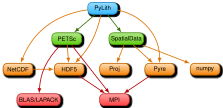
\includegraphics[width=4in]{implementation/figs/packages}
  \caption{PyLith dependencies. PyLith makes direct use of several
    other packages, some of which have their own dependencies.}
  \label{fig:pylith:dependencies}
\end{figure}

PyLith is written in two programming languages. High-level code is
written in Python; this rich, expressive interpreted language with
dynamic typing reduces development time and permits flexible addition
of user-contributed modules. This high-level code makes use of Pyre, a
science-neutral simulation framework developed at Caltech by Michael
Aivazis, to link the modules together at runtime and gather
user-input. Low-level code is written in C++, providing fast execution
while still allowing an object-oriented implementation. This low-level
code relies on PETSc for finite-element data structures, time-stepping
algorithms, and solvers. We use SWIG to create Python bindings for the
C++ objects.

In writing PyLith 1.0, the code was designed to be object-oriented and
modular. Each type of module is accessed through a specified interface
(set of functions). This permits adding, replacing, and rewriting
modules without affecting other parts of the code. This code structure
simplifies code maintenance and development. Extending the set of code
features is also easier, since developers can create new modules
derived from the existing ones.

The current code design leverages Pyre and PETSc extensively. Pyre
glues together the various modules used to construct a simulation and
specify the parameters. Most of the PyLith source code pertains to
implementing the geodynamics, such as the governing equations, bulk
rheology, boundary conditions, and earthquake rupture via slip on
faults.

Nemesis (Pyre subpackage) allows PyLith to run Python using the
Message Passing Interface (MPI) for parallel processing. Additional,
indirect dependencies (see Figure \vref{fig:pylith:dependencies})
include numpy (efficient operations on numerical arrays in Python),
Proj.4 (geographic projections).

During development we implement three levels of testing: (1) unit
testing, which occurs at the class/function level, (2) testing via the
Method of Manufactured Solutions to test the finite-element
implementation of the governing equations, and (3) full-scale testing,
which involves complete PyLith simulations. We run these tests
throughout the development cycle to expose bugs and isolate their
origin. As additional changes are made to the code, the tests are
rerun to help prevent introduction of new bugs.

Additionally, we use community benchmarks, such as developed through
the Southern California Earthquake Center for crustal deformation and
dynamic rupture to determine the relative local and global error (see
Chapter \vref{sec:benchmarks}).

\section{Pyre}

Pyre is an object-oriented environment capable of specifying and launching
numerical simulations on multiple platforms, including Beowulf-class
parallel computers and grid computing systems. Pyre allows the binding
of multiple components such as solid and fluid models used in Earth
science simulations, and different meshers. The Pyre framework enables
the elegant setup, modification and launching of massively parallel
solver applications.

\begin{figure}[htbp]
  \includegraphics[width=4in]{intro/figs/pyre_overview}
  \caption{Pyre Architecture. The integration framework is a set of
    cooperating abstract services.}
  \label{fig:Pyre:Architecture}
\end{figure}

Pyre is a framework, a combination of software and design philosophy
that promotes the reuse of code. In the context of frameworks and
object-oriented programming, Pyre can be thought of as a collection of
classes and the way their instances interact.  Programming
applications based on Pyre will look similar to those written in any
other object-oriented language. 

The Pyre framework incorporates features aimed at enabling the
scientific non-expert to perform tasks easily without hindering the
expert. Target features for end users allow complete and intuitive
simulation specification, reasonable defaults, consistency checks of
input, good diagnostics, easy access to remote facilities, and status
monitoring. Target features for developers include easy access to user
input, a shorter development cycle, and good debugging support.


\section{PETSc}

PyLith 2.x and later make use of a set of data structures and routines
in PETSc called \object{DMPlex}, which is still under active
development. \object{DMPlex} provides data structures and routines for
for representing and manipulating computational meshes, and it greatly
simplifies finite-element computations.\object{DMPlex} represents the
topology of the domain. Zero volume elements are inserted along all
fault surfaces to implement kinematic (prescribed) or dynamic
(constitutive model) implementations of fault slip. Material
properties and other parameters are represented as scalar and vector
fields over the mesh using vectors to store the values and sections to
map vertices, edges, faces, and cells to indices in the vector. For
each problem, functions are provided to calculate the residual and its
Jacobian.  All numerical integration is done in these functions, and
parallel assembly is accomplished using the get/set closure paradigm
of the \object{DMPlex} framework.

PETSc \url{www-unix.mcs.anl.gov/petsc/petsc-as}, the Portable,
Extensible Toolkit for Scientific computation, provides a suite of
routines for parallel, numerical solution of partial differential
equations for linear and nonlinear systems with large, sparse systems
of equations.  PETSc includes time-stepping algorithms and solvers
that implement a variety of Newton and Krylov subspace methods. It can
also interface with many external packages, including ESSL, MUMPS,
Matlab, ParMETIS, PVODE, and Hypre, thereby providing additional
solvers and interaction with other software packages.

PETSc includes interfaces for FORTRAN 77/90, C, C++, and Python for
nearly all of the routines, and PETSc can be installed on most Unix
systems. Users can use PETSc parallel matrices, vectors, and other
data structures for most parallel operations, eliminating the need for
explicit calls to Message Passing Interface (MPI) routines. Many
settings and options can be controlled with PETSc-specific
command-line arguments, including selection of preconditions, solvers,
and generation of performance logs.


\section{Finite-Element Implementation User Interface}

In specifying simulation parameters, some details of the
finite-element implementation using the PETSc \object{DMPlex} is
exposed to the user. In this section we describe the data structures
to give the user greater context for understanding what the parameters
mean.

\tip{See the dveloper guide in Chapter \vref{cha:developer} for a
  detailed discussion of the implementation and organization of the
  PyLith code.}

\subsection{Fields and Subfields}

Finite-element coefficients for the finite-element basis functions
(sometimes thought of as the values at vertices, on edges and faces,
or in cells) are stored in a \object{Field}. A \object{Field} is
composed of a \object{Section}, which associates the points (vertices,
edges, faces, and cells) with the finite-element coefficients, and a
\object{Vec}, which is a vector storing the finite-element
coefficients. A \object{Field} may hold a single subfield, such as
displacement, or it may hold several subfields, such as the density,
shear modulus, and bulk modulus for an isotropic, linear elastic
material.

Spatial discretization is specified for each subfield. That is, each subfield
within a \object{Field} can have a different discretization. For
example, a displacement field may use a second order discretization
while a pressure field may use a first order discretization. If we
have uniform material properties, we use a zero order discretization
(uniform values within a cell) to reduce the storage requirements.

The two main types of fields are the solution field and auxiliary
fields.

\subsubsection{Solution Field}

The solution field contains all of the finite-element coefficients
corresponding to the problem solution. As discussed in the
multiphysics finite-element formulation in
Section~\label{sec:multiphysics:formulation}, if the governing
equations have multiple unknowns, such as displacement and fluid
pressure for poroelasticity, then the solution field will have
multiple subfields.  See Section \vref{sec:solution:user:interface} for
details of the user interface and predefined containers for common
subfield collections.

\subsubsection{Auxiliary Field}

We specify parameters for materials, boundary conditions, and fault
interfaces using fields we refer to as the ``auxiliary'' fields.  Each
parameter (scalar, vector, tensor, or other) is held in a separate
subfield. We also store state variables in the auxiliary field, with
each state variable as a different subfield. This provides a single
container for the collection of spatially varying parameters while
maintaining the flexibility to specify the discretization of each
parameter separately. 

\subsubsection{Discretization}

The discretization of the field is given in terms of the topology
(vertices, edges, faces, and cells) associated with the field and the
basis order and quadrature order. The basis order refers to the
highest order in the basis functions. For example, a basis order of 0
has just a constant and a basis order of 2 for a polynomial basis has
constant, linear, and quadratic terms.

\warning{Currently, the quadrature order {\bf MUST} be the same for
  all subfields in a simulation. This restriction may be relaxed in
  the future. PyLith will check this and indicate if a subfield has a
  quadrature order that does not match the first solution subfield.}


% End of file


\chapter{Running PyLith}

Figure \ref{fig:pylith:workflow} shows the workflow for running PyLith.
There are essentially three main inputs needed to run a problem with
PyLith:
\begin{enumerate}
\item Mesh information. This includes the topology of the finite-element
mesh (coordinates of vertices and how the vertices are connected into
cells), a material identifier for each cell, and sets of vertices
associated with boundary conditions, faults, and output (for subsets
of the mesh). This information can be provided using the PyLith mesh
ASCII format (see Chapter \ref{cha:Tutorials} for examples and Section
\ref{sec:MeshIOAscii} for the format specification) or by importing
the information from the LaGriT or CUBIT meshing packages (see Chapter
\ref{cha:Tutorials} for examples).
\item A set of parameters describing the problem. These parameters describe
the type of problem to be run, solver information, time-stepping information,
boundary conditions, materials, etc. This information can be provided
from the command-line or by using a \texttt{.cfg.}
\item Databases specifying the material property values and boundary condition
values to be used. Arbitrarily complex spatial variations in boundary
and fault conditions and material properties may be given in the spatial
database (see Chapter \ref{cha:Tutorials} for examples and Appendix
\ref{sec:Spatialdata:SimpleIOAscii} for the format specification).
\end{enumerate}
PyLith writes solution information, such as solution fields and state
variables, to either VTK files or HDF5/Xdmf files. ParaView and Visit
can read both types of files. Post-processing of output is generally
performed using HDF5 files accessed via a Python script and the h5py
package or a Matlab script.

\noindent \begin{center}
\begin{figure}[H]
\noindent \begin{centering}
\includegraphics[width=5in]{runpylith/figs/runpylith} 
\par\end{centering}

\caption{PyLith requires a finite-element mesh (three different mechanisms
for generating a mesh are currently supported), simulation parameters,
and spatial databases (defining the spatial variation of various parameters).
PyLith writes the solution output to either VTK or HDF5/Xdmf files,
which can be visualized with ParaView or Visit. Post-processing is
generally done using the HDF5 files with Python or Matlab scripts.}


\label{fig:pylith:workflow} 
\end{figure}

\par\end{center}


\section{Defining the Simulation}

The parameters for PyLith are specified as a hierarchy or tree of
modules. The application assembles the hierarchy of modules from user
input and then calls the \texttt{main} function in the top-level module
in the same manner as a C or C++ program. The behavior of the application
is determined by the modules included in the hierarchy as specified
by the user. The Pyre framework provides the interface for defining
this hierarchy. Pyre properties correspond to simple settings in the
form of strings, integers, and real numbers. Pyre facilities correspond
to software modules. Facilities may have their own facilities (branches
in the tree) and any number of properties. See Figure \ref{fig:Pyre:Architecture}
for the general concept of Pyre facilities and properties. The top-level
object is the PyLith application with three facilities: \texttt{mesher},
\texttt{problem}, and \texttt{petsc}. The \texttt{mesher} specifies
how to import the mesh, the \texttt{problem} specifies the physical
properties, boundary conditions, etc., and \texttt{petsc} is used
to specify PETSc settings. Appendix \ref{cha:components} contains
a list of the components provided by PyLith and spatialdata.


\subsection{\label{sec:setting:parameters}Setting PyLith Parameters}

There are several methods for setting input parameters for the \texttt{pylith}
executable: via the command line or by using a text file in \texttt{.cfg}
or \texttt{.pml} format. Both facilities and properties have default
values provided, so you only need to set values when you want to deviate
from the default behavior.


\subsubsection{Units}

All dimensional parameters require units. The units are specified
using Python and FORTRAN syntax, so square meters is m{*}{*}2. Whitespace
is not allowed in the string, for units and dimensioned quantities
are multiplied by the units string; for example, two meters per second
is 2.0{*}m/s. Available units are shown in Table \ref{tab:pyre:units}

\noindent \begin{center}
\begin{table}[H]
\centering{}\caption{\label{tab:pyre:units}Pyre supported units. Aliases are in parentheses.}
\begin{tabular}{|>{\raggedright}p{0.9in}|>{\raggedright}p{4in}|}
\hline 
\textbf{Scale} & \textbf{Available Units}\tabularnewline
\hline 
\hline 
length & meter (m), micrometer (um, micron), millimeter (mm), centimeter (cm),
kilometer (km), inch, foot, yard, mile\tabularnewline
\hline 
time & second (s), nanosecond (ns), microsecond (us), millisecond (ms), minute,
hour, day, year\tabularnewline
\hline 
mass & kilogram (kg), gram (g), centigram (cg), milligram (mg), ounce, pound,
ton\tabularnewline
\hline 
pressure & pascal (Pa), kPa, MPa, GPa, bar, millibar, atmosphere (atm)\tabularnewline
\hline 
\end{tabular}
\end{table}

\par\end{center}


\subsubsection{Using the Command Line}

The \texttt{-{}-help} command line argument displays links to useful
resources for learning PyLith.

Pyre uses the following syntax to change properties from the command
line. To change the value of a property of a component, use:
\begin{lyxcode}
-{}-{[}component{]}.{[}property{]}={[}value{]}
\end{lyxcode}
Each component is attached to a facility, so the option above can
also be written as: 
\begin{lyxcode}
-{}-{[}facility{]}.{[}property{]}={[}value{]}
\end{lyxcode}
Each facility has a default component attached to it. A different
component can be attached to a facility by:
\begin{lyxcode}
-{}-{[}facility{]}={[}new\_component{]}~
\end{lyxcode}
PyLith's command-line arguments can control Pyre and PyLith properties
and facilities, MPI settings, and PETSc settings. All PyLith-related
properties are associated with the \texttt{pylithapp} component. You
can get a list of all of these top-level properties along with a description
of what they do by running PyLith with the \texttt{-{}-help-properties}
command-line argument. To get information on user-configurable facilities
and components, you can run PyLith with the \texttt{-{}-help-components}
command-line argument. To find out about the properties associated
with a given component, you can run PyLith with the \texttt{-{}-{[}component{]}.help-properties}
flag:
\begin{lyxcode}
\$~pylith~-{}-problem.help-properties
\end{lyxcode}
Each component may also have sub-components associated with it:
\begin{lyxcode}
\$~pylith~-{}-~problem.help-components
\end{lyxcode}
By starting at the top-level components, you can determine the components
and properties at each level by working down to lower-level components:
\begin{lyxcode}
\$~pylith~-{}-problem.bc.help-components

\$~pylith~-{}-problem.bc.help-properties
\end{lyxcode}
Using the \texttt{-{}-help-components} and \texttt{-{}-help-properties}
flags for the various components and sub-components is a good way
to discover potential problems in a simulation.


\subsubsection{Using a \texttt{.cfg} File}

Entering all those parameters via the command line involves the risk
of typographical errors, which can lead to undesired results. You
will generally find it easier to write a brief \texttt{.cfg} input
file that contains the parameters. This file has a format similar
to a Windows INI file. The file is composed of one or more sections
which are formatted as follows:
\begin{lyxcode}
{[}pylithapp.subcomponent1.subcomponent2{]}

\#~this~is~a~comment

property1~=~value1

property2~=~value2~;~this~is~another~comment
\end{lyxcode}
We strongly recommend that you use \texttt{.cfg} files for your work.
The files are syntax-highlighted in the vim editor.


\subsubsection{Using a \texttt{.pml} File}

A \texttt{.pml} file is an XML file that specifies parameter values
in a highly structured format. It is composed of nested sections which
are formatted as follows:
\begin{lyxcode}
<component~name='component1'>

~~~~<component~name='component2'>

~~~~~~~~<property~name='property1'>value1</property>

~~~~~~~~<property~name='property2'>value2</property>

~~~~</component>

</component>
\end{lyxcode}
XML files are intended to be read and written by machines, not edited
manually by humans. The \texttt{.pml} file format is intended for
applications in which PyLith input files are generated by another
program, e.g., a GUI, web application, or a high-level structured
editor. This file format will not be discussed further here, but if
you are interested in using \texttt{.pml} files, note that \texttt{.pml}
files and \texttt{.cfg} files can be used interchangeably; in the
following discussion, a file with a \texttt{.pml} extension can be
substituted anywhere a \texttt{.cfg} file can be used.


\subsubsection{Specification and Placement of Configuration Files}

Configuration files may be specified on the command line:
\begin{lyxcode}
\$~pylith~example.cfg
\end{lyxcode}
In addition, the Pyre framework searches for configuration files named
\texttt{pylithapp.cfg} in several predefined locations. You may put
settings in any or all of these locations, depending on the scope
you want the settings to have:
\begin{enumerate}
\item \texttt{\$PREFIX/etc/pylithapp.cfg}, for system-wide settings;
\item \texttt{\$HOME/.pyre/pylithapp/pylithapp.cfg}, for user settings and
preferences;
\item the current directory (\texttt{./pylithapp.cfg}), for local overrides. \end{enumerate}
\begin{quote}
\textbf{\textcolor{red}{Warning}}: The Pyre framework will search
these directories for .cfg files matching the names of components
(for example, \texttt{timedependent.cfg, faultcohesivekin.cfg, greensfns.cfg,
pointforce.cfg}, etc) and attempt to assign all parameters in those
files to the respective component.
\end{quote}
Parameters given directly on the command line will override any input
contained in a configuration file. Configuration files given on the
command line override all others. The \texttt{pylithapp.cfg} files
placed in (3) will override those in (2), (2) overrides (1), and (1)
overrides only the built-in defaults.

All of the example problems are set up using configuration files in
the example directory, and specific problems are defined by including
the appropriate configuration file on the command-line. Referring
to the directory \texttt{examples/twocells/twohex8}, the following
configuration files are present:
\begin{lyxcode}
axialdisp.cfg

dislocation.cfg

pylithapp.cfg

sheardisp.cfg
\end{lyxcode}
The settings in pylithapp.cfg will be read automatically, and additional
settings are included by specifying one of the other files on the
command-line:
\begin{lyxcode}
\$~pylith~axialdisp.cfg
\end{lyxcode}
If you want to see what settings are being used, you can either examine
the \texttt{.cfg} files, or use the help flags as described above:
\begin{lyxcode}
\$~pylith~axialdisp.cfg~-{}-problem.help-components

\$~pylith~axialdisp.cfg~-{}-problem.help-properties

\$~pylith~axialdisp.cfg~-{}-problem.bc.help-components

\$~pylith~axialdisp.cfg~-{}-problem.bc.help-properties
\end{lyxcode}
This is generally a more useful way of determining problem settings,
since it includes default values as well as those that have been specified
in the \texttt{.cfg} file.


\subsubsection{List of PyLith Parameters (\texttt{pylithinfo})}

The Python application \texttt{pylithinfo} writes all of the current
parameters to a text file. The default name of the text file is \texttt{pylith\_parameters.txt}.
The usage synopsis is
\begin{lyxcode}
\$~pylithinfo~{[}-{}-verbose{]}~{[}-{}-fileout=pylith\_parameters.txt{]}~{[}PyLith~args{]}
\end{lyxcode}
where \texttt{-{}-verbose} (or \texttt{-v}) turns on printing the
descriptions of the properties and components as well as the location
where the current value was set, and \texttt{-{}-fileout=pylith\_parameters.txt}
(or \texttt{-o pylith\_parameters.txt}) sets the name of the output
file. The lines in the text file are indented to show the hierarchy
of the properties and components. 


\subsection{Mesh Information (\texttt{mesher})}

Geometrical and topological information for the finite element mesh
may be provided by exporting an Exodus II format file from CUBIT,
by exporting a GMV file and an accompanying Pset file from LaGriT,
or by specifying the information in PyLith mesh ASCII format. See
Chapter \ref{cha:Tutorials} for examples.

PyLith supports linear cells in 1D (Figure \ref{fig:1D-linear-elements}),
2D (Figure \ref{fig:2D-linear-elements}), and 3D (Figure \ref{fig:3D-linear-elements}).
The vertex ordering must follow the convention shown in Figures \ref{fig:1D-linear-elements}-\ref{fig:3D-linear-elements}.
PyLith no longer supports use of quadratic cells using the PyLith
ASCII mesh format. In the next release, we plan to support higher
order discretizations via PETSc finite-element features from meshes
with linear cells as input.

The mesh information defines the vertex coordinates and specifies
the vertices composing each cell in the mesh. The mesh information
must also define at least one set of vertices for which displacement
(Dirichlet) boundary conditions will be provided. In most realistic
problems, there will be several vertex groups, each with a unique
identifying label. For example, one group might define a surface of
the mesh where displacement (Dirichlet) boundary conditions will be
applied, another might define a surface where traction (Neumann) boundary
conditions will be applied, while a third might specify a surface
that defines a fault. Similarly, the mesh information contains cell
labels that define the material type for each cell in the mesh. For
a mesh with a single material type, there will only be a single label
for every cell in the mesh. See Chapters \ref{cha:material:models}
and \ref{cha:boundary:interface:conditions} for more detailed discussions
of setting the materials and boundary conditions.

\noindent \begin{center}
\begin{figure}[H]
\noindent \begin{centering}
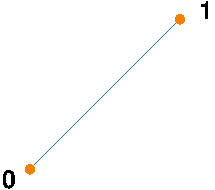
\includegraphics{runpylith/figs/bar2} 
\par\end{centering}

\caption{Linear bar cell available for 1D problems.}


\label{fig:1D-linear-elements} 
\end{figure}

\par\end{center}

\noindent \begin{center}
\begin{figure}[H]
\noindent \begin{centering}
\includegraphics{runpylith/figs/tri3}\hspace*{0.5in}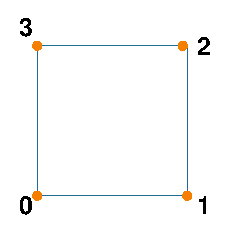
\includegraphics{runpylith/figs/quad4}
\par\end{centering}

\caption{Linear cells available for 2D problems are the triangle (left) and
the quadrilateral (right).}


\label{fig:2D-linear-elements} 
\end{figure}

\par\end{center}

\noindent \begin{center}
\begin{figure}[H]
\noindent \begin{centering}
\includegraphics{runpylith/figs/tet4}\hspace*{0.5in}\includegraphics{runpylith/figs/hex8}
\par\end{centering}

\caption{Linear cells available for 3D problems are the tetrahedron (left)
and the hexahedron (right).\label{fig:3D-linear-elements}}
\end{figure}

\par\end{center}


\subsubsection{Mesh Importer}

The default mesher component is MeshImporter, which provides the capabilities
of reading the mesh from files. The MeshImporter has several properties
and facilities:
\begin{description}
\item [{reorder\_mesh}] Reorder the vertices and cells using the reverse
Cuthill-McKee algorithm (default is False).
\item [{reader}] Reader for a given type of mesh (default is MeshIOAscii).
\item [{distributor}] Handles distribution of the mesh among processors.
\item [{refiner}] Perform global uniform mesh refinement after distribution
among processors (default is False).
\end{description}
Reordering the mesh so that vertices and cells connected topologically
also reside close together in memory improves overall performance
and can improve solver performance as well.
\begin{quote}
\textbf{\textcolor{red}{Warning}}\textcolor{red}{:} The coordinate
system associated with the mesh must be a Cartesian coordinate system.
This includes generic Cartesian coordinate systems as well as geographic
projections.
\end{quote}

\subsubsection{MeshIOAscii}

The MeshIOAscii object is intended for reading small, simple ASCII
files containing a mesh constructed by hand. We use this file format
extensively in the examples. Appendix \ref{sec:MeshIOAscii} describes
the format of the files. The properties and facilities of the MeshIOAscii
object include:
\begin{description}
\item [{filename}] Name of the mesh file.
\item [{coordsys}] Coordinate system associated with the mesh.
\end{description}

\subsubsection{\label{sec:MeshIOCubit}MeshIOCubit}

The MeshIOCubit object reads the NetCDF Exodus II files output from
CUBIT. Beginning with CUBIT 11.0, the names of the nodesets are included
in the Exodus II files and PyLith can use these nodeset names or revert
to using the nodeset ids. The properties and facilities associated
with the MeshIOCubit object are:
\begin{description}
\item [{filename}] Name of the Exodus II file.
\item [{use\_nodeset\_names}] Identify nodesets by name rather than id
(default is True).
\item [{coordsys}] Coordinate system associated with the mesh.
\end{description}

\subsubsection{\label{sec:MeshIOLagrit}MeshIOLagrit}

The MeshIOLagrit object is used to read ASCII and binary GMV and PSET
files output from LaGriT. PyLith will automatically detect whether
the files are ASCII or binary. We attempt to provide support for experimental
64-bit versions of LaGriT via flags indicating whether the FORTRAN
code is using 32-bit or 64-bit integers. The MeshIOLagrit properties
and facilities are:
\begin{description}
\item [{filename\_gmv}] Name of GMV file.
\item [{filename\_pset}] Name of the PSET file.
\item [{flip\_endian}] Flip the endian of values when reading binary files
(default is False).
\item [{io\_int32}] Flag indicating that PSET files use 32-bit integers
(default is True).
\item [{record\_header\_32bt}] Flag indicating FORTRAN record header is
32-bit (default is True)
\item [{coordsys}] Coordinate system associated with mesh.\end{description}
\begin{quote}
\textbf{\textcolor{red}{Warning}}: The PyLith developers have not
used LaGriT since around 2008 and the most recent release appears
to have been in 2010.
\end{quote}

\subsubsection{Distributor}

The distributor users a partitioner to compute which cells should
be placed on each processor, computes the overlap among the processors,
and then distributes the mesh among the processors. The type of partitioner
is set via PETSc settings. The properties and facilities of the Distributor
include:
\begin{description}
\item [{writer\_partition}] Flag indicating that the partition information
should be written to a file (default is False).
\item [{data\_writer}] Writer for partition information (default is DataWriterVTKMesh
for VTK output).
\end{description}
An example of setting the partitioner in a pylithapp.cfg file is:
\begin{lyxcode}
{[}pylithapp.petsc{]}

petscpartitioner~=~chaco~;~Options~are~'chaco'~(default)~and~'parmetis'.
\end{lyxcode}
METIS/ParMETIS are not included in the PyLith binaries due to licensing
issues. 


\subsubsection{Refiner}

The refiner is used to decrease node spacing by a power of two by
recursively subdividing each cell by a factor of two. In a 2D triangular
mesh a node is inserted at the midpoint of each edge, splitting each
cell into four cells (see Figure \ref{fig:uniform:refinement:2x}).
In a 2D quadrilateral mesh a node is inserted at the midpoint of each
edge and at the centroid of the cell, splitting each cell into four
cells. In a 3D tetrahedral mesh a node is inserted at the midpoint
of each edge, splitting each cell into eight cells. In a 3D hexahedral
mesh a node is inserted at the midpoint of each edge, the centroid
of each face, and at the centroid of the cell, splitting each cell
into eight cells.

\noindent \begin{center}
\begin{figure}[H]
\noindent \begin{centering}
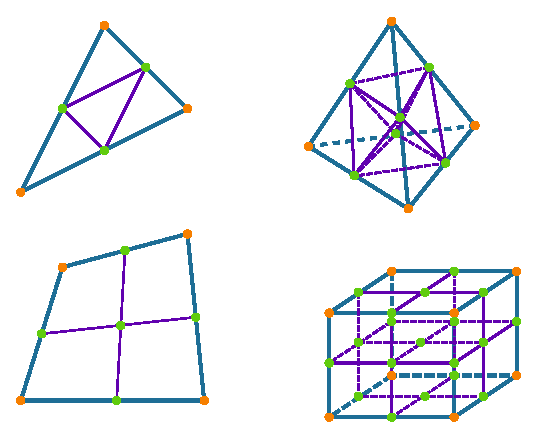
\includegraphics[scale=1.25]{runpylith/figs/refinement2x}
\par\end{centering}

\caption{Global uniform mesh refinement of 2D and 3D linear cells. The blue
lines and orange circles identify the edges and vertices in the original
cells. The purple lines and green circles identify the new edges and
vertices added to the original cells to refine the mesh by a factor
of two.\label{fig:uniform:refinement:2x}}
\end{figure}

\par\end{center}

Refinement occurs after distribution of the mesh among processors.
This allows one to run much larger simulations by (1) permitting the
mesh generator to construct a mesh with a node spacing largeer than
that needed in the simulation and (2) operations performed in serial
during the simulation setup phase, such as, adjusting the topology
to insert cohesive cells and distribution of the mesh among processors
uses this much smaller coarse mesh. For 2D problems the global mesh
refinement increases the maximum problem size by a factor of $4^{n}$,
and for 3D problems it increases the maximum problem size by a factor
of $8^{n}$, where $n$ is the number of recursive refinement levels.
For a tetrahedral mesh, the element quality decreases with refinement
so $n$ should be limited to 1-2.


\subsection{Problem Specification (\texttt{problem})}

The problem component specifies the basic parameters of the simulation,
including the physical properties, the boundary conditions, and interface
conditions (faults). The current release of PyLith contains two types
of problem, \texttt{TimeDependent} for use in static, quasi-static,
and dynamic simulations and \texttt{GreensFns} for computing static
Green's functions. The general facilities include:
\begin{description}
\item [{normalizer}] Scales used to nondimensionalize the problem (default
is NondimElasticQuasistatic).
\item [{materials}] Array of materials comprising the domain (default is
\texttt{{[}material{]}}).
\item [{bc}] Array of boundary conditions (default is none).
\item [{interfaces}] Array of interface conditions, i.e., faults (default
is none).
\item [{gravity\_field}] Gravity field used to construct body forces (default
is none).
\end{description}
The properties for each material group are:
\begin{description}
\item [{dimension}] Spatial dimension of the problem (default is 3)
\end{description}
An example of setting these parameters in a \texttt{.cfg} file for
a problem is:
\begin{lyxcode}
{[}pylithapp.timedependent{]}

dimension~=~3

normalizer~=~spatialdata.units.NondimElasticQuasistatic

materials~=~{[}elastic,viscoelastic{]}

bc~=~{[}boundary\_east,boundary\_bottom,boundary\_west{]}

interfaces~=~{[}SanAndreas,SanJacinto{]}

gravity\_field~=~spatialdata.spatialdb.GravityField
\end{lyxcode}

\subsubsection{Nondimensionalization}

PyLith nondimensionalizes all parameters provided by the user so that
the simulation solves the equations using nondimensional quantities.
This permits application of PyLith to problems across a vast range
of spatial and temporal scales. The scales used to nondimensionalize
the problem are length, pressure, density, and time. PyLith provides
two normalizer objects to make it easy to provide reasonable scales
for the nondimensionalization. The \texttt{NondimElasticQuasistatic}
normalizer (which is the default) has the following properties:
\begin{description}
\item [{length\_scale}] Length to nondimensionalize length (default is
1.0 km).
\item [{shear\_modulus}] Shear modulus to nondimensionalize pressure (default
is 3.0e+10 Pa).
\item [{relaxation\_time}] Relaxation time to nondimensionalize time (default
is 1.0 year).
\end{description}
An example of setting these parameters in a \texttt{.cfg} file for
a problem is:
\begin{lyxcode}
{[}pylithapp.timedependent.normalizer{]}

length\_scale~=~1.0{*}km

shear\_modules~=~3.0e+10{*}Pa

relaxation\_time~=~1.0{*}yr
\end{lyxcode}
The \texttt{NondimElasticDynamic} normalizer has the following properties:
\begin{description}
\item [{shear\_wave\_speed}] Shear wave speed used to nondimensionalize
length and pressure (default is 3.0 km/s).
\item [{mass\_density}] Mass density to nondimensionalize density and pressure
(default is 3.0e+3 kg/m$^{3}$).
\item [{wave\_period}] Period of seismic waves used to nondimensionalize
time (default is 1.0 s).
\end{description}
An example of setting these parameters in a \texttt{.cfg} file for
a problem is:
\begin{lyxcode}
{[}pylithapp.timedependent.normalizer{]}

shear\_wave\_speed~=~3.0{*}km/s

mass\_density~=~3.0e+3{*}kg/m{*}{*}3

wave\_period~=~1.0{*}s
\end{lyxcode}
The default nondimensionalization is reasonable for many problems;
however, it may be necessary to change the default values in some
cases. When doing this, keep in mind that the nondimensionalization
generally applies to the minimum values encountered for a problem.
For example, in a quasistatic problem, the \texttt{length\_scale}
should be on the order of the minimum cell size. Similarly, the \texttt{relaxation\_time}
should be on the order of the minimum relaxation time.


\subsection{Finite-Element Integration Settings}

PyLith uses numerical quadrature to evaluate the finite-element integrals
for the residual and system Jacobian (see Chapter \ref{cha:Governing-Equations}).
PyLith employs FIAT (finite element automatic tabulator) to compute
the basis functions and their derivatives at the quadrature points
for various quadrature schemes and cell shapes. The parameters for
Lagrange cells (lines, quadrilaterals, hexahedra) are specified using
the FIATLagrange object, whereas the parameters for Simplex cells
(lines, triangles, tetrahedra) are specified using the FIATSimplex
object. Both objects use the same set of parameters and PyLith will
setup the basis functions and quadrature scheme appropriately for
the two families of cells. The quadrature scheme and basis functions
must be set for each material and boundary condition involving finite-element
integrations (Dirichlet boundary conditions are constraints and do
not involve integrations). Furthermore, the integration schemes can
be set independently. The current version of PyLith supports basis
functions with linear variations in the field (P1); support for higher
order cells will be added in the future. The properties for the FIATLagrange
and FIATSimplex objects are
\begin{description}
\item [{dimension}] Dimension of the cell (0,1,2,3; default is 3).
\item [{degree}] Degree of the finite-element cell (default is 1).
\item [{order}] Order of quadrature rule (default is degree+1); hardwired
to be equal to degree for faults.
\item [{collocate\_quad}] Collocate quadrature points with vertices (default
is False); hardwired to True for faults.
\end{description}
See Section \ref{sec:material:parameters} for an example of setting
these properties for a material.


\subsection{\label{sec:petsc:options}PETSc Settings (\texttt{petsc})}

In quasti-static problems with implicit time-stepping, PyLith relies
on PETSc for the linear algebra computations, including linear Krylov
subspace solvers and nonlinear solvers. For dynamic problems, lumping
the mass matrix and using explicit time-stepping is much more efficient;
this permits solving the linear system with a trivial solver so we
do not use a PETSc solver in this case (see Section \ref{sec:solvers}).

PETSc options can be set in \texttt{.cfg} files in sections beginning
with \texttt{{[}pylithapp.petsc{]}}. The options of primary interest
in the case of PyLith are shown in Table~\ref{tab:petsc:options:defaults}.
PETSc options are used to control the selection and settings for the
solvers underlying the SolverLinear and SolverNonlinear objects discussed
in Section \ref{sec:solvers}. A very wide range of elasticity problems
in quasi-static simulations can be solved with reasonable runtimes
by replacing the default Jacobi preconditioner with the Additive Schwarz
Method (ASM) using Incomplete LU (ILU) factorization by default (see
Table~\ref{tab:petsc:options:recommended}). A more advanced set
of solver settings that may provide better performance in many elasticity
problems are given in Table \ref{tab:petsc:options:advanced}. These
are available in \texttt{\$PYLITH\_DIR/share/settings/solver\_fault\_fieldsplit.cfg.}
These settings are limited to problems where we store the stiffness
matrix as a nonsymmetric sparse matrix and require additional settings
for the formulation,
\begin{lyxcode}
{[}pylithapp.timedependent.formulation{]}

split\_fields~=~True

use\_custom\_constraint\_pc~=~True~;~Use~only~if~problem~contains~a~fault

matrix\_type~=~aij\end{lyxcode}
\begin{quote}
\textbf{\textcolor{red}{Warning:}}\textbf{ }These settings are only
available if you build PETSc with the ML package. These features are
included in the PyLith binary packages.

\textbf{\textcolor{red}{Warning:}}\textbf{ }The split fields and algebraic
multigrid preconditioning currently fails in problems with a nonzero
null space. This most often occurs when a problem contains multiple
faults that extend through the entire domain and create subdomains
without any Dirichlet boundary conditions. The current workaround
is to use the Additive Schwarz preconditioner without split fields.
See Section \ref{sec:Troubleshooting} for the error message encountered
in this situation. 
\end{quote}
These more advanced settings allow the displacement fields and Lagrange
multipliers for fault tractions to be preconditioned separately. This
usually results in a much stronger preconditioner. In simulations
with fault slip, the degrees of freedom associated with the Lagrange
multipliers should be preconditioned with a custom preconditioner
that uses a diagonal approximation of the Schur complement.

\noindent \begin{center}
\begin{table}[H]
\centering{}\caption{\label{tab:petsc:options:defaults}Useful command-line arguments for
setting PETSc options.}
\begin{tabular}{|>{\raggedright}p{1.2in}|>{\centering}m{0.6in}|>{\raggedright}p{3.8in}|}
\hline 
\textbf{Property} & \textbf{Default Value} & \textbf{Description}\tabularnewline
\hline 
\hline 
\texttt{log\_view} & \textit{false} & Print logging objects and events.\tabularnewline
\hline 
\texttt{ksp\_monitor} & \textit{false} & Dump preconditioned residual norm to stdout.\tabularnewline
\hline 
\texttt{ksp\_view} & \textit{false} & Print linear solver parameters. \tabularnewline
\hline 
\texttt{ksp\_rtol} & \textit{1.0e-05} & Convergence tolerance for relative decrease in residual norm.\tabularnewline
\hline 
\texttt{snes\_monitor} & \textit{false} & Dump residual norm to stdout for each nonlinear solve iteration.\tabularnewline
\hline 
\texttt{snes\_view} & \textit{false} & Print nonlinear solver parameters.\tabularnewline
\hline 
\texttt{snes\_rtol} & \textit{1.0e-5} & Convergence tolerance for relative decrease in residual norm.\tabularnewline
\hline 
\texttt{pc\_type} & \textit{jacobi} & Set preconditioner type. See \href{http://www.mcs.anl.gov/petsc/petsc-as/documentation/linearsolvertable.html}{PETSc documentation}
for a list of all preconditioner types. \tabularnewline
\hline 
\texttt{ksp\_type} & \textit{gmres} & Set linear solver type. See \href{http://www.mcs.anl.gov/petsc/petsc-as/documentation/linearsolvertable.html}{PETSc documentation}
for a list of all solver types.\tabularnewline
\hline 
\end{tabular}
\end{table}
\begin{table}[H]
\centering{}\caption{\label{tab:petsc:options:recommended}PETSc options that provide moderate
performance in a wide range of quasi-static elasticity problems.}
\begin{tabular}{|>{\raggedright}p{2in}|>{\centering}m{0.75in}|>{\raggedright}p{3in}|}
\hline 
\textbf{Property} & \textbf{Value} & \textbf{Description}\tabularnewline
\hline 
\hline 
\texttt{pc\_type} & \textit{asm} & Additive Schwarz method.\tabularnewline
\hline 
\texttt{ksp\_type} & \textit{gmres} & GMRES method from Saad and Schultz.\tabularnewline
\hline 
\texttt{sub\_pc\_factor\_shift\_type} & \emph{nonzero} & Turn on nonzero shifting for factorization.\tabularnewline
\hline 
\texttt{ksp\_max\_it} & \emph{100} & Maximum number of iterations permitted in linear solve. Depends on
problem size.\tabularnewline
\hline 
\texttt{ksp\_gmres\_restart} & \textit{50} & Number of iterations after which Gram-Schmidt orthogonalization is
restarted.\tabularnewline
\hline 
\texttt{ksp\_rtol} & \textit{1.0e-08} & Linear solve convergence tolerance for relative decrease in residual
norm.\tabularnewline
\hline 
\texttt{ksp\_atol} & \textit{\emph{1.0e-12}} & Linear solve convergence tolerance for absolute value of residual
norm.\tabularnewline
\hline 
\texttt{ksp\_converged\_reason} & \textit{true} & Indicate why iterating stopped in linear solve.\tabularnewline
\hline 
\texttt{snes\_max\_it} & \textit{100} & Maximum number of iterations permitted in nonlinear solve. Depends
on how nonlinear the problem is.\tabularnewline
\hline 
\texttt{snes\_rtol} & \textit{1.0e-08} & Nonlinear solve convergence tolerance for relative decrease in residual
norm.\tabularnewline
\hline 
\texttt{snes\_atol} & \textit{1.0e-12} & Nonlinear solve convergence tolerance for absolute value of residual
norm.\tabularnewline
\hline 
\texttt{snes\_converged\_reason} & \textit{true} & Indicate why iterating stopped in nonlinear solve.\tabularnewline
\hline 
\end{tabular}
\end{table}

\par\end{center}

\noindent \begin{center}
\begin{table}[H]
\centering{}\caption{\label{tab:petsc:options:advanced}PETSc options used with split fields
algebraic multigrid preconditioning that often provide improved performance
in quasi-static elasticity problems with faults.}
\begin{tabular}{|>{\raggedright}p{2.75in}|>{\centering}m{0.75in}|>{\raggedright}p{2.5in}|}
\hline 
\textbf{Property} & \textbf{Value} & \textbf{Description}\tabularnewline
\hline 
\hline 
\texttt{\footnotesize{}fs\_pc\_type} & \textit{field\_split} & Precondition fields separately.\tabularnewline
\hline 
\texttt{\footnotesize{}fs\_pc\_use\_amat} & \textit{true} & Use diagonal blocks from the true operator, rather than the preconditioner.\tabularnewline
\hline 
\texttt{\footnotesize{}fs\_pc\_fieldsplit\_type} & \textit{multiplicative} & Apply each field preconditioning in sequence, which is stronger than
all-at-once (additive).\tabularnewline
\hline 
\texttt{\footnotesize{}fs\_fieldsplit\_displacement\_pc\_type} & \textit{ml} & Multilevel algebraic multigrid preconditioning using Trilinos/ML via
PETSc.\tabularnewline
\hline 
\texttt{\footnotesize{}fs\_fieldsplit\_lagrange\_multiplier\_pc\_type} & \textit{jacobi} & Jacobi preconditioning for Lagrange multiplier block\tabularnewline
\hline 
\texttt{\footnotesize{}fs\_fieldsplit\_displacement\_ksp\_type} & \textit{preonly} & Apply only the preconditioner.\tabularnewline
\hline 
\texttt{\footnotesize{}fs\_fieldsplit\_lagrange\_multiplier\_ksp\_type} & \textit{preonly} & Apply only the preconditioner.\tabularnewline
\hline 
\end{tabular}
\end{table}

\par\end{center}


\subsubsection{Model Verification with PETSc Direct Solvers}

It is often useful to apply a direct solver so that solver convergence
is decoupled from model verification for the purposes of testing.
Unfortunately, the traditional LU factorization solvers cannot be
directly applied in PyLith due to the saddle-point formulation used
to accomodate the fault slip constraints. However, we can combine
an LU factorization of the displacement sub-block with a full Schur
complement factorization using the PETSc FieldSplit preconditioner.
If the solver for the Schur complement S is given a very low tolerance,
this is effectively a direct solver. The options given below will
construct this solver in PyLith. These settings are available in\texttt{}~\\
\texttt{\$PYLITH\_DIR/share/settings/solver\_fault\_exact.cfg}.
\begin{lyxcode}
{[}pylithapp.timedependent.formulation{]}

split\_fields~=~True

matrix\_type~=~aij



{[}pylithapp.petsc{]}

fs\_pc\_type~=~fieldsplit

fs\_pc\_use\_amat~=~True

fs\_pc\_fieldsplit\_type~=~schur

fs\_pc\_fieldsplit\_schur\_factorization\_type~=~full

fs\_fieldsplit\_displacement\_ksp\_type~=~preonly

fs\_fieldsplit\_displacement\_pc\_type~=~lu

fs\_fieldsplit\_lagrange\_multiplier\_pc\_type~=~jacobi

fs\_fieldsplit\_lagrange\_multiplier\_ksp\_type~=~gmres

fs\_fieldsplit\_lagrange\_multiplier\_ksp\_rtol~=~1.0e-11
\end{lyxcode}

\section{Time-Dependent Problem}

This type of problem applies to transient static, quasi-static, and
dynamic simulations. The time-dependent problem adds the \texttt{formulation}
facility to the general-problem. The formulation specifies the time-stepping
formulation to integrate the elasticity equation. PyLith provides
several alternative formulations, each specific to a different type
of problem.
\begin{description}
\item [{Implicit}] Implicit time stepping for static and quasi-static problems
with infinitesimal strains. The implicit formulation neglects inertial
terms (see Section \ref{eq:elasticity:integral:quasistatic}). 
\item [{ImplicitLgDeform}] Implicit time stepping for static and quasi-static
problems including the effects of rigid body motion and small strains.
This formulation requires the use of the nonlinear solver, which is
selected automatically.
\item [{Explicit}] Explicit time stepping for dynamic problems with infinitesimal
strains and lumped system Jacobian. The cell matrices are lumped before
assembly, permitting use of a vector for the diagonal system Jacobian
matrix. The built-in lumped solver is selected automatically.
\item [{ExplicitLgDeform}] Explicit time stepping for dynamic problems
including the effects of rigid body motion and small strains. The
cell matrices are lumped before assembly, permitting use of a vector
for the diagonal system Jacobian matrix. The built-in lumped solver
is selected automatically.
\item [{ExplicitTri3}] Optimized elasticity formulation for linear triangular
cells with one point quadrature for dynamic problems with infinitesimal
strains and lumped system Jacobian. The built-in lumped solver is
selected automatically.
\item [{ExplicitTet4}] Optimized elasticity formulation for linear tetrahedral
cells with one point quadrature for dynamic problems with infinitesimal
strains and lumped system Jacobian.The built-in lumped solver is selected
automatically.
\end{description}
In many quasi-static simulations it is convenient to compute a static
problem with elastic deformation prior to computing a transient response.
Up through PyLith version 1.6 this was hardwired into the Implicit
Forumulation as advancing from time step $t=-\Delta t$ to $t=0$,
and it could not be turned off. PyLith now includes a property, \texttt{elastic\_prestep}
in the TimeDependent component to turn on/off this behavior (the default
is to retain the previous behavior of computing the elastic deformation). 
\begin{quote}
\textbf{\textcolor{red}{Warning:}}\textbf{ }Turning off the elastic
prestep calculation means the model only deforms when an \texttt{\textit{increment}}
in loading or deformation is applied, because the time-stepping formulation
is implemented using the increment in displacement.
\end{quote}
The TimeDependent properties and facilities include
\begin{description}
\item [{elastic\_preset}] If true, perform a static calculation with elastic
behavior before time stepping (default is True).
\item [{formulation}] Formulation for solving the partial differential
equation.
\item [{progress\_monitor}] Simple progress monitor via text file.
\end{description}
An example of setting the properties and components in a .cfg file
is
\begin{lyxcode}
{[}pylithapp.timedependent{]}

formulation~=~pylith.problems.Implicit~;~default

progres\_monitor~=~pylith.problems.ProgressMonitorTime~;~default

elastic\_preset~=~True~;~default
\end{lyxcode}
The formulation value can be set to the other formulations in a similar
fashion. 


\subsection{Time-Stepping Formulation}

The explicit and implicit time stepping formulations use a common
set of facilities and properties. The facilities include
\begin{description}
\item [{time\_step}] Time step size specification (default is uniform time
step).
\item [{solver}] Type of solver to use (default is SolverLinear).
\item [{output}] Array of output managers for output of the solution (default
is {[}output{]}).
\item [{jacobian\_viewer}] Viewer to dump the system Jacobian (sparse matrix)
to a file for analysis (default is PETSc binary).
\end{description}
The formulation properties include
\begin{description}
\item [{matrix\_type}] Type of PETSc matrix for the system Jacobian (sparse
matrix, default is symmetric, block matrix with a block size of 1).
\item [{view\_jacobian}] Flag to indicate if system Jacobian (sparse matrix)
should be written to a file (default is false).
\item [{split\_fields}] Split solution field into a displacement portion
(fields 0..ndim-1) and a Lagrange multiplier portion (field ndim)
to permit application of sophisticated PETSc preconditioners (default
is false).
\end{description}
An example of setting these parameters in a \texttt{.cfg} file is
\begin{lyxcode}
{\footnotesize{}{[}pylithapp.timedependent.formulation{]}}{\footnotesize \par}

{\footnotesize{}time\_step~=~pylith.problems.TimeStepUniform}{\footnotesize \par}

{\footnotesize{}solver~=~pylith.problems.SolverLinear~;~Nonlinear~solver~is~pylith.problems.SolverNonlinear}{\footnotesize \par}

{\footnotesize{}output~=~{[}domain,ground\_surface{]}}{\footnotesize \par}

{\footnotesize{}matrix\_type~=~sbaij~;~To~use~a~non-symmetric~sparse~matrix,~set~it~to~aij}{\footnotesize \par}

{\footnotesize{}view\_jacobian~=~false}{\footnotesize \par}
\end{lyxcode}

\subsection{Numerical Damping in Explicit Time Stepping}

In explicit time-stepping formulations for elasticity, boundary conditions
and fault slip can excite short waveform elastic waves that are not
accurately resolved by the discretization. We use numerical damping
via an artificial viscosity\cite{Knopoff:Ni:2001,Day:Ely:2002} to
reduce these high frequency oscillations. In computing the strains
for the elasticity term in equation \ref{eq:elasticity:integral:dynamic:t},
we use an adjusted displacement rather than the actual displacement,
where 
\begin{equation}
\vec{u}^{adj}(t)=\vec{u}(t)+\eta^{*}\Delta t\vec{\dot{u}}(t),
\end{equation}
$\vec{u}^{adj}(t)$ is the adjusted displacement at time t, $\vec{u}(t)$is
the original displacement at time (t), $\eta^{*}$is the normalized
artificial viscosity, $\Delta t$ is the time step, and $\vec{\dot{u}}(t)$
is the velocity at time $t$. The default value for the normalized
artificial viscosity is 0.1. We have found values in the range 0.1-0.4
sufficiently suppress numerical noise while not excessively reducing
the peak velocity. An example of setting the normalized artificial
viscosity in a \texttt{.cfg} file is
\begin{lyxcode}
{[}pylithapp.timedependent.formulation{]}

norm\_viscosity~=~0.2
\end{lyxcode}

\subsection{\label{sec:solvers}Solvers}

PyLith supports three types of solvers. The linear solver, SolverLinear,
corresponds to the PETSc KSP solver and is used in linear problems
with linear elastic and viscoelastic bulk constitutive models and
kinematic fault ruptures. The nonlinear solver, SolverNonlinear, corresponds
to the PETSc SNES solver and is used in nonlinear problems with nonlinear
viscoelastic or elastoplastic bulk constitutive models, dynamic fault
ruptures, or problems involving finite strain (small strain formulation).
The lumped solver (SolverLumped) is a specialized solver used with
the lumped system Jacobian matrix. The options for the PETSc KSP and
SNES solvers are set via the top-level PETSc options (see Section
\ref{sec:petsc:options} and the PETSc documentation \url{www.mcs.anl.gov/petsc/petsc-as/documentation/index.html}).


\subsection{\label{sub:Time-Stepping}Time Stepping}

PyLith provides three choices for controlling the time step in time-dependent
simulations. These include (1) a uniform, user-specified time step
(which is the default), (2) user-specified time steps (potentially
nonuniform), and (3) automatically calculated (potentially nonuniform)
time steps. The procedure for automatically selecting time steps requires
that the material models provide a reasonable estimate of the time
step for stable time integration. In general, quasi-static simulations
with viscoelastic materials should use automatically calculated time
steps and dynamic simulations should use a uniform, user-specified
time step. Note that all three of the time stepping schemes make use
of the computed stable time step (see \ref{sub:Stable-time-step}).
When using user-specified time steps, the value is checked against
the computed stable time step. The automatically calculated time step
comes from the computed stable time step.
\begin{quote}
\textbf{\textcolor{red}{Warning:}} Varying the time step within a
simulation requires recomputing the Jacobian of the system whenever
the time step changes, which can greatly increase the runtime if the
time-step size changes frequently.
\end{quote}

\subsubsection{Uniform, User-Specified Time Step}

With a uniform, user-specified time step, the user selects the time
step that is used over the entire duration of the simulation. If this
value exceeds the computed stable time step at any time, PyLith will
terminate with an error. The properties for the uniform, user-specified
time step are:
\begin{description}
\item [{total\_time}] Time duration for simulation (default is 0.0 s).
\item [{start\_time}] Start time for simulation (default is 0.0 s)
\item [{dt}] Time step for simulation.
\end{description}
An example of setting a uniform, user-specified time step in a \texttt{.cfg}
file is:
\begin{lyxcode}
{[}pylithapp.problem.formulation{]}

time\_step~=~pylith.problems.TimeStepUniform~;~Default~value



{[}pylithapp.problem.formulation.time\_step{]}

total\_time~=~1000.0{*}year

dt~=~0.5{*}year
\end{lyxcode}

\subsubsection{Nonuniform, User-Specified Time Step}

The nonuniform, user-specified, time-step implementation allows the
user to specify the time steps in an ASCII file (see Section \ref{sec:FileFormat:TimeStepUser}
for the format specification of the time-step file). If the total
duration exceeds the time associated with the time steps, then a flag
determines whether to cycle through the time steps or to use the last
specified time step for the time remaining. Similar to the uniform
time step, if the user-specified time step size exceeds the computed
stable time step at any time, PyLith will terminate with an error.
The properties for the nonuniform, user-specified time step are:
\begin{description}
\item [{total\_time}] Time duration for simulation.
\item [{filename}] Name of file with time-step sizes.
\item [{loop\_steps}] If true, cycle through time steps, otherwise keep
using last time-step size for any time remaining.
\end{description}
An example of setting the properties for nonuniform, user-specified
time steps in a \texttt{.cfg} file is:
\begin{lyxcode}
{[}pylithapp.problem.formulation{]}

time\_step~=~pylith.problems.TimeStepUser~;~Change~the~time~step~algorithm



{[}pylithapp.problem.formulation.time\_step{]}

total\_time~=~1000.0{*}year

filename~=~timesteps.txt

loop\_steps~=~false~;~Default~value
\end{lyxcode}

\subsubsection{Nonuniform, Automatic Time Step}

This time-step implementation automatically calculates a time step
size based on the constitutive model and rate of deformation. As a
result, this choice for choosing the time step relies on accurate
calculation of a stable time step within each finite-element cell
by the constitutive models. To provide some control over the time-step
selection, the user can control the frequency with which a new time
step is calculated, the time step to use relative to the value determined
by the constitutive models, and a maximum value for the time step.
Note that the stability factor allows the computed time step size
to exceed the computed stable time step. A stability factor of 1.0
would provide a time step size equal to the stable time step, while
a value of 2.0 (default value) would provide a time step size equal
to 1/2 the stable time step. Caution should be used when adjusting
the stability factor to values less than 1.0, as the large time step
size may result in inaccurate solutions. The properties for controlling
the automatic time-step selection are:
\begin{description}
\item [{total\_time}] Time duration for simulation.
\item [{max\_dt}] Maximum time step permitted.
\item [{adapt\_skip}] Number of time steps to skip between calculating
new stable time step.
\item [{stability\_factor}] Safety factor for stable time step (default
is 2.0).
\end{description}
An example of setting the properties for the automatic time step in
a \texttt{.cfg} file is:
\begin{lyxcode}
{[}pylithapp.problem.formulation{]}

time\_step~=~pylith.problems.TimeStepAdapt~;~Change~the~time~step~algorithm



{[}pylithapp.problem.formulation.time\_step{]}

total\_time~=~1000.0{*}year

max\_dt~=~10.0{*}year

adapt\_skip~=~10~;~Default~value

stability\_factor~=~2.0~;~Default~value
\end{lyxcode}

\section{Green's Functions Problem}

This type of problem applies to computing static Green's functions
for elastic deformation. The \texttt{GreensFns} problem specializes
the time-dependent facility to the case of static simulations with
slip impulses on a fault. The default formulation is the Implicit
formulation and should not be changed as the other formulations are
not applicable to static Green's functions. In the output files, the
deformation at each ``time step'' is the deformation for a different
slip impulse. The properties provide the ability to select which fault
to use for slip impulses. The only fault component available for use
with the \texttt{GreensFns} problem is the \texttt{FaultCohesiveImpulses}
component discussed in Section \ref{sec:fault:cohesive:impulses}.
The \texttt{GreensFns} properties amd facilities include:
\begin{description}
\item [{fault\_id}] Id of fault on which to impose slip impulses.
\item [{formulation}] Formulation for solving the partial differential
equation.
\item [{progress\_monitor}] Simple progress monitor via text file.
\end{description}
An example of setting the properties for the GreensFns problem in
a \texttt{.cfg} file is:
\begin{lyxcode}
{[}pylithapp{]}

problem~=~pylith.problems.GreensFns~;~Change~problem~type~from~the~default



{[}pylithapp.greensfns{]}

fault\_id~=~100~;~Default~value

formulation~=~pylith.problems.Implicit~;~default

progres\_monitor~=~pylith.problems.ProgressMonitorTime~;~default

\end{lyxcode}
\begin{quote}
\textbf{\textcolor{red}{Warning:}} The \texttt{GreensFns} problem
generates slip impulses on a fault. The current version of PyLith
requires that impulses can only be applied to a single fault and the
fault facility must be set to \texttt{FaultCohesiveImpulses}.
\end{quote}

\section{Progress Monitors}
\begin{quotation}
\texttt{\textcolor{red}{New in v2.1.0.}}
\end{quotation}
The progress monitors make it easy to monitor the general progress
of long simulations, especially on clusters where stdout is not always
easily accessible. The progress monitors update a simulation's current
progress by writing information to a text file. The information includes
time stamps, percent completed, and an estimate of when the simulation
will finish. 


\subsection{ProgressMonitorTime}

This is the default progress monitor for time-stepping problems. The
monitor calculates the percent completed based on the time at the
current time step and the total simulated time of the simulation,
not the total number of time steps (which may be unknown in simulations
with adaptive time stepping). The \texttt{ProgressMonitorTime} properties
include:
\begin{description}
\item [{update\_percent}] Frequency (in percent) of progress updates.
\item [{filename}] Name of output file.
\item [{t\_units}] Units for simulation time in output.
\end{description}
An example of setting the properties in a .\texttt{cfg} file is:
\begin{lyxcode}
{[}pylithapp.problem.progressmonitor{]}

update\_percent~=~5.0~;~default

filename~=~progress.txt~;~default

t\_units~=~year~;~default
\end{lyxcode}

\subsection{ProgressMonitorStep}

This is the default progress monitor for problems with a specified
number of steps, such as Green's function problems. The monitor calculates
the percent completed based on the number of steps (e.g., Green's
function impulses completed). The ProgressMonitorStep propertiles
include:
\begin{description}
\item [{update\_percent}] Frequency (in percent) of progress updates.
\item [{filename}] Name of output file.
\end{description}
An example of setting the properties in a .\texttt{cfg} file is:
\begin{lyxcode}
{[}pylithapp.problem.progressmonitor{]}

update\_percent~=~5.0~;~default

filename~=~progress.txt~;~default
\end{lyxcode}

\section{\label{sec:spatial:databases}Databases for Boundaries, Interfaces,
and Material Properties}

Once the problem has been defined with PyLith parameters, and the
mesh information has been provided, the final step is to specify the
boundary conditions and material properties to be used. The mesh information
provides labels defining sets of vertices to which boundary conditions
or fault conditions will be applied, as well as cell labels that will
be used to define the material type of each cell. For boundary conditions,
the \texttt{.cfg} file is used to associate boundary condition types
and spatial databases with each vertex group (see Chapter \ref{cha:boundary:interface:conditions}).
For materials, the \texttt{.cfg} file is used to associate material
types and spatial databases with cells identified by the material
identifier (see Figure \ref{fig:Material-models}).

The spatial databases define how the boundary conditions or material
property values vary spatially, and they can be arbitrarily complex.
The simplest example for a material database would be a mesh where
all the cells of a given type have uniform properties (``point''
or 0D variation). A slightly more complex case would be a mesh where
the cells of a given type have properties that vary linearly along
a given direction (``line'' or 1D variation). In more complex models,
the material properties might have different values at each point
in the mesh (``volume'' or 3D variation). This might be the case,
for example, if the material properties are provided by a database
of seismic velocities and densities. For boundary conditions the simplest
case would be where all vertices in a given group have the same boundary
condition parameters (``point'' or 0D variation). A more complex
case might specify a variation in the conditions on a given surface
(``area'' or 2D variation). This sort of condition might be used,
for example, to specify the variation of slip on a fault plane. The
examples discussed in Chapter \ref{cha:Tutorials} also contain more
information regarding the specification and use of the spatial database
files.


\subsection{SimpleDB Spatial Database}

In most cases the default type of spatial database for faults, boundary
conditions, and materials is \texttt{SimpleDB}. Spatial database files
provide specification of a field over some set of points. There is
no topology associated with the points. Although multiple values can
be specified at each point with more than one value included in a
search query, the interpolation of each value will be done independently.
Time dependent variations of a field are not supported in these files.
Spatial database files can specify spatial variations over zero, one,
two, and three dimensions. Zero dimensional variations correspond
to uniform values. One-dimensional spatial variations correspond to
piecewise linear variations, which need not coincide with coordinate
axes. Likewise, two-dimensional spatial variations correspond to variations
on a planar surface (which need not coincide with the coordinate axes)
and three-dimensional spatial variations correspond to variations
over a volume. In one, two, or three dimensions, queries can use a
``nearest value'' search or linear interpolation.

The spatial database files need not provide the data using the same
coordinate system as the mesh coordinate system, provided the two
coordinate systems are compatible. Examples of compatible coordinate
systems include geographic coordinates (longitude/latitude/elevation),
and projected coordinates (e.g., coordinates in a transverse Mercator
projection). Spatial database queries use the Proj.4 Cartographic
Projections library \url{proj.maptools.org} to convert between coordinate
systems, so a large number of geographic projections are available
with support for converting between NAD27 and WGS84 horizontal datums
as well as several other frequently used datums. Because the interpolation
is done in the coordinate system of the spatial database, geographic
coordinates should only be used for very simple datasets, or undesirable
results will occur. This is especially true when the spatial database
coordinate system combines latitude, longitude, and elevation in meters
(longitude and latitude in degrees are often much smaller than elevations
in meters leading to distorted ``distance'' between locations and
interpolation).

SimpleDB uses a simple ASCII file to specify the variation of values
(e.g., displacement field, slip field, physical properties) in space.
The file format is described in Section \ref{sec:Spatialdata:SimpleIOAscii}.
The tutorials in Chapter \ref{cha:Tutorials} use SimpleDB files to
specify the values for the boundary conditions,  physical properties,
and fault slip.

As in the other Pyre objects, spatial database objects contain parameters
that can be set from the command line or using \texttt{.cfg or .pml}
files. The parameters for a spatial database are:
\begin{description}
\item [{label}] Label for the database, which is used in diagnostic messages.
\item [{query\_type}] Type of search query to perform. Values for this
parameter are ``linear'' and ``nearest'' (default).
\item [{iohandler}] Database importer. Only one importer is implemented,
so you do not need to change this setting.
\item [{iohandler.filename}] Filename for the spatial database.
\end{description}
An example of setting these parameters in a \texttt{.cfg} file is:
\begin{lyxcode}
label~=~Material~properties

query\_type~=~linear

iohandler.filename~=~mydb.spatialdb


\end{lyxcode}

\subsection{UniformDB Spatial Database}

The SimpleDB spatial database is quite general, but when the values
are uniform, it is often easier to use the UniformDB spatial database
instead. With the UniformDB, you specify the values directly either
on the command line or in a parameter-setting (\texttt{.cfg}) file.
On the other hand, if the values are used in more than one place,
it is easier to place the values in a SimpleDB file, because they
can then be referred to using the filename of the spatial database
rather than having to repeatedly list all of the values on the command
line or in a parameter-setting (\texttt{.cfg}) file. The Pyre properties
for a UniformDB are:
\begin{description}
\item [{values}] Array of names of values in spatial database
\item [{data}] Array of values in spatial database
\end{description}

\subsubsection{Example}

Specify the physical properties of a linearly elastic, isotropic material
in a \texttt{pylithapp.cfg} file. The data values are dimensioned
with the appropriate units using Python syntax.
\begin{lyxcode}
{\footnotesize{}{[}pylithapp.timedependent.materials.material{]}}{\footnotesize \par}

{\footnotesize{}db\_properties~=~spatialdata.spatialdb.UniformDB~;~Set~the~db~to~a~UniformDB}{\footnotesize \par}

{\footnotesize{}db\_properties.values~=~{[}vp,vs,density{]}~;~Set~the~names~of~the~values~in~the~database}{\footnotesize \par}

{\footnotesize{}db\_properties.data~=~{[}5773.5{*}m/s,~3333.3{*}m/s,~2700.0{*}kg/m{*}{*}3{]}~;~Set~the~values~in~the~database}{\footnotesize \par}
\end{lyxcode}

\subsubsection{ZeroDispDB}

The ZeroDispDB is a a special case of the UniformDB for the Dirichlet
boundary conditions. The values in the database are the ones requested
by the Dirichlet boundary conditions, \texttt{displacement-x}, \texttt{displacement-y},
and \texttt{displacement-z}, and are all set to zero. This makes it
trivial to set displacements to zero on a boundary. The examples discussed
in Chapter \ref{cha:Tutorials} use this database.


\subsection{SimpleGridDB Spatial Database}

The SimpleGridDB object provides a much more efficient query algorithm
than SimpleDB in cases with a orthogonal grid. The points do not need
to be uniformly spaced along each coordinate direction. Thus, in contrast
to the SimpleDB there is an implicit topology. Nevertheless, the points
can be specified in any order, as well as over a lower-dimension than
the spatial dimension. For example, one can specify a 2-D grid in
3-D space provided that the 2-D grid is aligned with one of the coordinate
axes. 

SimpleGridDB uses a simple ASCII file to specify the variation of
values (e.g., displacement field, slip field, physical properties)
in space. The file format is described in Section \ref{sec:Spatialdata:SimpleGrid}. 

As in the other Pyre objects, spatial database objects contain parameters
that can be set from the command line or using \texttt{.cfg or .pml}
files. The parameters for a spatial database are:
\begin{description}
\item [{label}] Label for the database, which is used in diagnostic messages.
\item [{query\_type}] Type of search query to perform. Values for this
parameter are ``linear'' and ``nearest'' (default).
\item [{filename}] Filename for the spatial database.
\end{description}
An example of setting these parameters in a \texttt{.cfg} file is:
\begin{lyxcode}
label~=~Material~properties

query\_type~=~linear

filename~=~mydb\_grid.spatialdb


\end{lyxcode}

\subsection{\label{sub:SCECCVMH-Impl}SCEC CVM-H Spatial Database}

Although the SimpleDB implementation is able to specify arbitrarily
complex spatial variations, there are existing databases for physical
properties, and when they are available, it is desirable to access
these directly. One such database is the SCEC CVM-H database, which
provides seismic velocities and density information for much of southern
California. Spatialdata provides a direct interface to this database.
See Section \ref{sec:Tutorial-Two-tet4-geoproj} for an example of
using the SCEC CVM-H database for physical properties of an elastic
material. The interface is known to work with versions 5.2 and 5.3
of the SCEC CVM-H. Setting a minimum wave speed can be used to replace
water and very soft soils that are incompressible or nearly incompressible
with stiffer, compressible materials. The Pyre properties for the
SCEC CVM-H are:
\begin{description}
\item [{data\_dir}] Directory containing the SCEC CVM-H data files
\item [{min\_vs}] Minimum shear wave speed. Corresponding minimum values
for the dilatational wave speed (Vp) and density are computed. Default
value is 500 m/s.
\item [{squash}] Squash topography/bathymetry to sea level (make the earth's
surface flat)
\item [{squash\_limit}] Elevation above which topography is squashed (geometry
below this elevation remains undistorted)
\end{description}

\subsubsection{Example}

Specify the physical properties of a linearly elastic, isotropic material
using the SCEC CVM-H in a \texttt{pylithapp.cfg} file.
\begin{lyxcode}
{\small{}{[}pylithapp.timedependent.materials.material{]}}{\small \par}

{\small{}db\_properties~=~spatialdata.spatialdb.SCECCVMH~;~Set~the~database~to~the~SCEC~CVM-H}{\small \par}

{\small{}db\_properties.data\_dir~=~/home/johndoe/data/sceccvm-h/vx53~;~Directory~containing}~\\
{\small{}the~database~data~files}{\small \par}

{\small{}db\_properties.min\_vs~=~500{*}m/s}{\small \par}

{\small{}db\_properties.squash~=~True~;~Turn~on~squashing}{\small \par}

{\small{}db\_properties.squash\_limit~=~-1000.0~;~Only~distort~the~geometry~above~z~=~-1~km~in~}~\\
{\small{}flattening~the~earth}{\small \par}
\end{lyxcode}

\subsection{CompositeDB Spatial Database}

For some problems, a boundary condition or material property may have
subsets with different spatial variations. One example would be when
we have separate databases to describe the elastic and inelastic bulk
material properties for a region. In this case, it would be useful
to have two different spatial databases, e.g., a seismic velocity
model with Vp, Vs, and density values, and another database with the
inelastic physical properties. We can use the \texttt{CompositeDB}
spatial database for these cases. An example would be:
\begin{lyxcode}
{[}pylithapp.timedependent.materials.maxwell{]}

label~=~Maxwell~material

id~=~1

db\_properties~=~spatialdata.spatialdb.CompositeDB

db\_properties.db\_A~=~spatialdata.spatialdb.SCECCVMH

db\_properties.db\_B~=~spatialdata.spatialdb.SimpleDB

quadrature.cell~=~pylith.feassemble.FIATSimplex

quadrature.cell.dimension~=~3

~

{[}pylithapp.timedependent.materials.maxwell.db\_properties{]}

values\_A~=~{[}density,vs,vp{]}

db\_A.label~=~Elastic~properties~from~CVM-H

db\_A.data\_dir~=~/Users/willic3/geoframe/tools/vx53/bin

db\_A.squash~=~False

values\_B~=~{[}viscosity{]}

db\_B.label~=~Vertically~varying~Maxwell~material

db\_B.iohandler.filename~=~../spatialdb/mat\_vert\_var\_maxwell.spatialdb
\end{lyxcode}
Here we have specified a \texttt{CompositeDB} where the elastic properties
(\texttt{density}, \texttt{vs}, \texttt{vp}) are given by the SCEC
CVM-H, and \texttt{viscosity} is described by a \texttt{SimpleDB}
(\texttt{mat\_vert\_var\_maxwell.spatialdb}). The user must first
specify \texttt{db\_properties} as a \texttt{CompositeDB}, and must
then give the two components of this database (\texttt{SCECCVMH} and
\texttt{SimpleDB}). The values to query in each of these databases
is also required. This is followed by the usual parameters for each
of the spatial databases. The \texttt{CompositeDB} provides a flexible
mechanism for specifying material properties or boundary conditions
where the variations come from two different sources.


\subsection{Time History Database}

The time history database specifies the temporal variation in the
amplitude of a field associated with a boundary condition. It is used
in conjunction with spatial databases to provide spatial and temporal
variation of parameters for boundary conditions. The same time history
is applied to all of the locations, but the time history may be shifted
with a spatial variation in the onset time and scaled with a spatial
variation in the amplitude. The time history database uses a simple
ASCII file which is simpler than the one used by the SimpleDB spatial
database. The file format is described in Section \ref{sec:Spatialdata:TimeHistoryIO}. 

As in the other Pyre objects, spatial database objects contain parameters
that can be set from the command line or using \texttt{.cfg or .pml}
files. The parameters for a spatial database are:
\begin{description}
\item [{label}] Label for the time history database, which is used in diagnostic
messages.
\item [{filename}] Filename for the time history database.
\end{description}
An example of setting these parameters in a \texttt{.cfg} file is:
\begin{lyxcode}
label~=~Displacement~time~history

filename~=~mytimehistory.timedb
\end{lyxcode}

\section{Labels and Identifiers for Materials, Boundary Conditions, and Faults}

For materials, the ``label'' is a string used only for error messages.
The ``id'' is an integer that corresponds to the material identifier
in LaGriT (itetclr) and CUBIT (block id). The id also tags the cells
in the mesh for associating cells with a specific material model and
quadrature rule. For boundary conditions, the ``label'' is a string
used to associate groups of vertices (psets in LaGriT and nodesets
in CUBIT) with a boundary condition. Some mesh generators use strings
(LaGriT) to identify groups of nodes while others (CUBIT) use strings
and integers. The default behavior in PyLith is to use strings to
identify groups for both LaGriT and CUBIT meshes, but the behavior
for CUBIT meshes can be changed to use the nodeset id (see Section
\ref{sec:MeshIOCubit}). PyLith 1.0 had an ``id'' for boundary conditions,
but we removed it from subsequent releases because it was not used.
For faults the ``label'' is used in the same manner as the ``label''
for boundary conditions. That is, it associates a string with a group
of vertices (pset in LaGriT and nodeset in CUBIT). The fault ``id''
is a integer used to tag the cohesive cells in the mesh with a specific
fault and quadrature rule. Because we use the fault ``id'' to tag
cohesive cells in the mesh the same way we tag normal cells to materials,
it must be unique among the faults as well as the materials.


\section{PyLith Output}

PyLith currently supports output to VTK and HDF5/Xdmf files, which
can be imported directly into a number of visualization tools, such
as ParaView, Visit, and MayaVi. The HDF5 files can also be directly
accessed via Matlab and PyTables. PyLith 1.1 significantly expanded
the information available for output, including fault information
and state variables. Output of solution information for the domain,
faults, materials, and boundary conditions is controlled by an output
manager for each module. This allows the user to tailor the output
to the problem. By default PyLith will write a number of files. Diagnostic
information for each fault and material is written into a separate
file as are the solution and state variables for the domain, each
fault, and each material. For a fault the diagnostic fields include
the final slip, the slip initiation time, and the fault normal vector.
For a material the diagnostic fields include the density and the elastic
constants. Additional diagnostic information can be included by setting
the appropriate output parameters. See Chapters \ref{cha:material:models}
and \ref{cha:boundary:interface:conditions} for more information
on the available fields and the next section for output parameters.
The other files for each fault and material include solution information
at each time step where output was requested (also customizable by
the user). For a fault the solution information includes the slip
and the change in tractions on the fault surface. For a material the
solution information includes the total strain and stress. For some
materials fields for additional state variables may be available.
For output via VTK files, each time step is written to a separate
file, whereas for HDF5 files all of the time steps for a given domain,
fault, or material are written into the same file. A single Xdmf metadata
file is created for each HDF5 file.


\subsection{Output Manager}

The OutputManager object controls the type of files written, the fields
included in the output, and how often output is written. PyLith includes
some specialized OutputManagers that prescribe what fields are output
by default. In some cases, additional fields are available but not
included by default. For example, in 3D problems, the along-strike
and up-dip directions over the fault surface can be included in the
diagnostic information. These are not included by default, because
1D problems have neither an along-strike nor up-dip direction and
2D problems do not have an up-dip direction.


\subsubsection{Output Manager Parameters}

The parameters for the OutputManager are:
\begin{description}
\item [{output\_freq}] Flag indicating whether to write output based on
the time or number of time steps since the last output. Permissible
values are ``time\_step'' and ``skip'' (default).
\item [{time\_step}] Minimum time between output if \texttt{output\_freq}
is set to ``time\_step''.
\item [{skip}] Number of time steps between output if \texttt{output\_freq}
is set to ``skip''. A value of 0 means every time step is written.
\item [{writer}] Writer for data (VTK writer or HDF5 writer).
\item [{coordsys}] Coordinate system for vertex coordinates (currently
ignored).
\item [{vertex\_filter}] Filter to apply to all vertex fields (see Section
\ref{sub:vertex:field:filters}).
\item [{cell\_filter}] Filter to apply to all cell fields (see Section
\ref{sub:cell:field:filters}).
\end{description}
An example of setting the output parameters for a material in a \texttt{.cfg}
file is
\begin{lyxcode}
{[}pylithapp.timedependent.materials.elastic.output{]}

output\_freq~=~time\_step

time\_step~=~1.0{*}yr

cell\_filter~=~pylith.meshio.CellFilterAvg

cell\_info\_fields~=~{[}density{]}~;~limit~diagnostic~data~to~density

cell\_data\_fields~=~{[}total-strain,stress{]}~;~default

writer.filename~=~dislocation-elastic.vtk
\end{lyxcode}

\subsubsection{Output Over Subdomain}

Output of the solution over the entire domain for large problems generates
very large data files. In some cases one is primarily interested in
the solution over the ground surface. PyLith supports output of the
solution on any boundary of the domain by associating an output manager
with a group of vertices corresponding to the surface of the boundary.
As with several of the boundary conditions, the boundary must be a
simply-connected surface. The \texttt{OutputSolnSubset} is the specialized
OutputManager that implements this feature and, by default, includes
the displacement field in the output. In addition to the \texttt{OutputManager}
parameters, the \texttt{OutputSolnSubset} includes:
\begin{description}
\item [{label}] Label of group of vertices defining boundary surface.
\item [{vertex\_data\_fields}] Names of vertex data fields to output (default
is {[}``displacements''{]}).
\end{description}

\subsection{\label{sec:output:points}Output at Arbitrary Points}

In many situations with recorded observations, one would like to extract
the solution at the same locations as the recorded observation. Rather
than forcing the finite-element discretization to be consistent with
the observation points, PyLith includes a specialized output manager,
\texttt{OutputSolnPoints}, to interpolate the solution to arbitrary
points. By default, the output manager will include the displaceent
time histories in the output. The locations are specified in a text
file. In addition to the \texttt{OutputManager} parameters, the \texttt{OutputSolnSubset}
includes:
\begin{description}
\item [{vertex\_data\_fields}] Names of vertex data fields to output (default
is {[}``displacements''{]}).
\item [{reader}] Reader for points list (default is \texttt{PointsList}).
\item [{writer}] Writer for output (default is \texttt{DataWriterVTKPoints}).
In most cases users will want to use the \texttt{}~\linebreak{}
\texttt{DataWriterHDF5}.
\end{description}

\subsubsection{PointsList Reader}

This object corresponds to a simple text file containing a list of
points (one per line) where output is desired. See \ref{sec:FileFormat:PointsList}
for file format specifications. The points are specified in the coordinate
system specified by OutputSolnPoints. The coordinates will be transformed
into the coordinate system of the mesh prior to interpolation. The
properties available to customize the behavior of \texttt{PointsList}
are:
\begin{description}
\item [{filename}] Names of file containing list of points.
\item [{comment\_delimiter}] Delimiter at beginning of line to identify
comments (default is \#).
\item [{value\_delimiter}] Delimiter used to separate values (default is
whitespace).
\end{description}

\subsection{Output Field Filters}

Output fields may not directly correspond to the information a user
desires. For example, the default output for the state variables includes
the physical properties at each quadrature point. Most visualization
packages cannot handle cell fields with multiple points in a cell
(the locations of the points within the cell are not included in the
data file). In order to reduce the field to a single point within
the cell, we would like to average the values. This is best done within
PyLith before output, because it reduces the file size and the quadrature
information provides the information necessary (the weights of the
quadrature points) to compute the appropriate average over the cell.


\subsubsection{\label{sub:vertex:field:filters}Vertex Field Filters}

Currently the only filter available for vertex fields computes the
magnitude of a vector at each location. Most visualization packages
support this operation, so this filter is not very useful.
\begin{description}
\item [{VertexFilterVecNorm}] Computes the magnitude of a vector field
at each location.
\end{description}

\subsubsection{\label{sub:cell:field:filters}Cell Field Filters}

Most users will want to apply a filter to cell fields to average the
fields over the cell, producing values at one location per cell for
visualization.
\begin{description}
\item [{CellFilterAvg}] Compute the weighted average of the values within
a cell. The weights are determined from the quadrature associated
with the cells.
\end{description}

\subsection{VTK Output}

PyLith writes legacy (non-XML) VTK files. These are simple files with
vertex coordinates, the mesh topology, and fields over vertices and/or
cells. Each time step is written to a different file. The time stamp
is included in the filename with the decimal point removed. This allows
automatic generation of animations with many visualization packages
that use VTK files. The default time stamp is the time in seconds,
but this can be changed using the normalization constant to give a
time stamp in years, tens of years, or any other value.


\subsubsection{DataWriterVTK Parameters}

The parameters for the VTK writer are:
\begin{description}
\item [{filename}] Name of VTK file
\item [{time\_format}] C-style format string for time stamp in filename.
The decimal point in the time stamp will be removed for compatibility
with VTK visualization packages that provide seamless animation of
data from multiple VTK files.
\item [{time\_constant}] Value used to normalize time stamp in VTK files
(default is 1.0 s).
\end{description}

\subsection{\label{sub:HDF5/Xdmf-Output}HDF5/Xdmf Output}

HDF5 files provide a flexible framework for storing simulation data
with datasets in groups logically organized in a tree structure analogous
to files in directories. HDF5 output offers parallel, multi-dimensional
array output in binary files, so it is much faster and more convenient
than the VTK output which uses ASCII files and separate files for
each time step. Standards for organizing datasets and groups in HDF5
files do not exist for general finite-element software in geodynamics.
Consequently, PyLith uses its own simple layout show in Figure \ref{fig:hdf5:layout}.
In order for visualization tools, such as ParaView, to determine which
datasets to read and where to find them in the hierarchy of groups
within the HDF5 file, we create an Xdmf (eXtensible Data Model and
Format, \url{www.xdmf.org}) metadata file that provides this information.
This file is written when PyLith closes the HDF5 file at the end of
the simulation. In order to visualize the datasets in an HDF5 file,
one simply opens the corresponding Xdmf file (the extension is \texttt{.xmf})
in ParaView or Visit. The Xdmf file contains the relative path to
the HDF5 file so the files can be moved but must be located together
in the same directory. 
\begin{quote}
\textbf{\textcolor{red}{Note:}}\textbf{ }The Xdmf format supports
representation of two- and three-dimensional coordinates of points,
scalar fields, and three-dimensional vector and tensor fields but
not two-dimensional vector or tensor fields. Consequently, for two-dimensional
vector fields we build a three-component vector from the two-component
vector (x and y components) and a separate zero scalar field (z component).
For tensor fields, we create a scalar field for each of the tensor
components, adding the component as a suffix to the name of the field.
\end{quote}
\noindent \begin{center}
\begin{figure}[H]
\noindent \begin{centering}
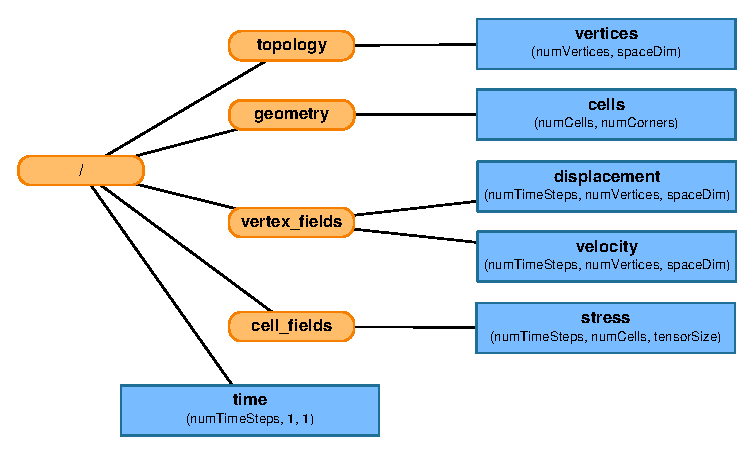
\includegraphics{runpylith/figs/hdf5layout}
\par\end{centering}

\caption{General layout of a PyLith HDF5 file. The orange rectangles with rounded
corners identify the groups and the blue rectangles with sharp corners
identify the datasets. The dimensions of the data sets are shown in
parentheses. Most HDF5 files will contain either \texttt{vertex\_fields}
or \texttt{cell\_fields} but not both. \label{fig:hdf5:layout}}
\end{figure}

\par\end{center}

See Table \ref{tab:material-model-statevars} in Section \ref{sec:material:parameters}
for a table of component values for tensor output in HDF5 files. To
avoid confusion about the ordering of components for tensor data,
we separate the components in the Xdmf file.

HDF5 files do not contain self-correcting features that allow a file
to be read if part of a dataset is corrupted. This type of error can
occur if a job terminates abnormally in the middle or at the end of
a simulation on a large cluster or other parallel machine. Fortunately,
HDF5 also offers the ability to store datasets in external binary
files with the locations specified by links in the HDF5 file. Note
that the use of external data files results in one data file per dataset
in addition to the HDF5 and Xdmf files. The external data files use
the name of the HDF5 file with the dataset name added to the prefix
and the \texttt{.h5} suffix replaced by \texttt{.dat}. The HDF5 files
include relative paths to the external data files, so these files
can also be moved, but they, too, must be kept together in the same
directory. This provides a more robust method of output because one
can generate an HDF5 file associated with the uncorrupted portions
of the external data files should an error occur. Currently, PyLith
does not include a utility to do this, but we plan to add one in a
future release. Thus, there are two options when writing PyLith output
to HDF5 files: (1) including the datasets directly in the HDF5 files
themselves or (2) storing the datasets in external binary files with
just metadata in the HDF5 files. Both methods provide similar performance
because they will use MPI I/O if it is available. 
\begin{quote}
\textbf{\textcolor{red}{Warning:}}\textbf{ }Storing the datasets within
the HDF5 file in a parallel simulation requires that the HDF5 library
be configured with the \texttt{-{}-enable-parallel} option. The binary
PyLith packages include this feature and it is a default setting in
building HDF5 via the PyLith Installer.
\end{quote}
Accessing the datasets for additional analysis or visualization is
nearly identical in the two methods because the use of external data
files is completely transparent to the user except for the presence
of the additional files. Note that in order for ParaView to find the
HDF5 and external data files, it must be run from the same relative
location where the simulation was run. For example, if the simulation
was run from a directory called ``work'' and the HDF5/Xdmf files
were written to ``work/output'', then ParaView should be run from
the ``work'' directory. See Table \ref{tab:material-model-statevars}
in Section \ref{sec:material:parameters} for a table of component
values for tensor output.


\subsubsection{HDF5 Utilities}

HDF5 includes several utilities for examining the contents of HDF5
files. \texttt{h5dump} is very handy for displaying the hierarchy,
dimensions of datasets, attributes, and even the dataset values. 
\begin{quote}
Dump the entire HDF5 file to stdout (not practical or useful for large
files):
\begin{lyxcode}
h5dump~mydata.h5
\end{lyxcode}
Dump the hierarchy of an HDF5 file to stdout:
\begin{lyxcode}
h5dump~-n~mydata.h5
\end{lyxcode}
Dump the hierarchy with dataset dimensions and attributes to stdout:
\begin{lyxcode}
h5dump~-H~mydata.h5
\end{lyxcode}
Dump dataset 'vertices' in group '/geometry' to stdout:
\begin{lyxcode}
h5dump~-d~/geometry/vertices~mydata.h5
\end{lyxcode}
\end{quote}
We have also include a utility \texttt{pylith\_genxdmf} (see Section
\ref{sub:pylith_genxdmf}) that generates an appropriate Xdmf file
from a PyLith HDF5 file. This is very useful if you add fields to
HDF5 files in post-processing and wish to view the results in ParaView
or Visit.


\subsubsection{DataWriterHDF5 Parameters}

This HDF5 writer stores the datasets inside the HDF5 file and the
parameters are:
\begin{description}
\item [{filename}] Name of HDF5 file (the Xdmf filename is generated from
the same prefix).
\end{description}

\subsubsection{DataWriterHDF5Ext Parameters}

This HDF5 writer stores the datasets using external data files (a
more robust method for parallel runs) and the parameters are:
\begin{description}
\item [{filename}] Name of HDF5 file (the external dataset filenames and
the Xdmf filename are generated from the same prefix).
\end{description}
An example of changing the writer from the default VTK writer to the
HDF5 writer with external datasets for output over the domain in a
\texttt{.cfg} file is
\begin{lyxcode}
{[}pylithapp.timedependent.domain.output{]}

output\_freq~=~time\_step

time\_step~=~1.0{*}yr

cell\_data\_fields~=~{[}displacement,velocity{]}

writer~=~pylith.meshio.DataWriterHDF5Ext

writer.filename~=~dislocation.h5
\end{lyxcode}

\section{Tips and Hints\label{sec:Tips:Hints}}


\subsection{Tips and Hints For Running PyLith}
\begin{itemize}
\item Examine the examples for a problem similar to the one you want to
run and dissect it in detail.
\item Start with a uniform-resolution coarse mesh to debug the problem setup.
Increase the resolution as necessary to resolve the solution fields
of interest (resolving stresses/strains may require a higher resolution
than that for resolving displacements).
\item Merge materials using the same material model. This will result in
only one VTK or HDF5 file for each material model rather than several
files.
\item The rate of convergence in quasi-static (implicit) problems can sometimes
be improved by renumbering the vertices in the finite-element mesh
to reduce the bandwidth of the sparse matrix. PyLith can use the reverse
Cuthill-McKee algorithm to reorder the vertices and cells.
\item If you encounter errors or warnings, run \texttt{pylithinfo} or use
the \texttt{-{}-help}, \texttt{-{}-help-components}, and \texttt{-{}-help-properties}
command-line arguments when running PyLith to check the parameters
to make sure PyLith is using the parameters you intended.
\item Use the \texttt{-{}-petsc.log\_}view, \texttt{-{}-petsc.ksp\_monitor},
\texttt{-{}-petsc.ksp\_view}, \texttt{}~\\
\texttt{-{}-petsc.ksp\_converged\_reason}, and \texttt{-{}-petsc.snes\_converged\_reason}
command-line arguments (or set them in a parameter file) to view PyLith
performance and monitor the convergence.
\item Turn on the journals (see the examples) to monitor the progress of
the code.
\end{itemize}

\subsection{Troubleshooting\label{sec:Troubleshooting}}
\begin{itemize}
\item Consult the PyLith FAQ webpage (\url{http://www.geodynamics.org/cig/community/workinggroups/short/workarea/pylith-wiki})
which contains a growing list of common problems and their corresponding
solutions.
\item \texttt{ImportError: liblapack.so.2: cannot open shared object file: No
such file or directory}\end{itemize}
\begin{quote}
PyLith cannot find one of the libraries. You need to set up your environment
variables (e.g., PATH, PYTHONPATH, and LD\_LIBRARY\_PATH) to match
your installation. If you are using the PyLith binary on Linux or
Mac OS X, run the command \texttt{source setup.sh }in the directory
where you unpacked the distribution. This will set up your environment
variables for you. If you are building PyLith from source, please
consult the instructions for building from source.\end{quote}
\begin{itemize}
\begin{singlespace}
\item \texttt{>\textcompwordmark{}> \{command line\}:: }~\\
\texttt{-{}- pyre.inventory(error) }~\\
\texttt{-{}- p4wd <- 'true' }~\\
\texttt{-{}- unrecognized property 'p4wd' }~\\
\texttt{>\textcompwordmark{}> \{command line\}:: }~\\
\texttt{-{}- pyre.inventory(error) }~\\
\texttt{-{}- p4pg <- 'true' }~\\
\texttt{-{}- unrecognized property ' p4pg'}\end{singlespace}
\end{itemize}
\begin{quote}
Verify that the `mpirun' command included in the PyLith package is
the first one on your PATH:

\texttt{\$ which mpirun}

If it is not, adjust your PATH environment variable accordingly.\end{quote}
\begin{itemize}
\item \texttt{\textquotedbl{}merlin.DistributionNotFound: Cheetah\textquotedbl{}
error}\end{itemize}
\begin{quote}
This error occurs when trying to use the 32-bit linux binary on some
64-bit linux systems. One of the Python packages PyLith uses does
not know how to determine the system architecture at runtime. The
workaround is:
\begin{enumerate}
\item Go to the \texttt{lib/python2.7/site-packages} directory.
\item Unzip \texttt{merlin-1.8-py2.7.egg} (if it is a file and not a directory).
\item Go to the merlin directory.
\item Edit \texttt{\_\_init\_\_.py}. Replace line 308 plat = get\_platform()
with plat = \textquotedbl{}linux-i686\textquotedbl{}
\item If \texttt{merlin-1.8-py2.7.egg} is a file, rezip merlin. Go to the
site-packages directory and enter \textquotedbl{}\texttt{zip -r merlin-1.8-py2.7.egg
merlin}\textquotedbl{}.
\end{enumerate}
\end{quote}
\begin{itemize}
\item \texttt{-{}- Solving equations.}~\\
\texttt{{[}0{]}PETSC ERROR: -{}-{}-{}-{}-{}-{}-{}-{}-{}-{}-{}-{}-{}-{}-{}-
Error Message -{}-{}-{}-{}-{}-{}-{}-{}-{}-{}-{}-{}-{}-{}-{}-{}-{}-{}-{}-{}-{}-{}-{}-{}-{}-{}-{}-{}-{}-{}-
}~\\
\texttt{{[}0{]}PETSC ERROR: Detected zero pivot in LU factorization}~\\
\texttt{ see http://www.mcs.anl.gov/petsc/petsc-as/documentation/faq.html\#ZeroPivot!}\end{itemize}
\begin{quote}
This usually occurs when the null space of the system Jacobian is
nonzero, such as the case of a problem without Dirichlet boundary
conditions on any boundary. If this arises when using the split fields
and algebraic multigrid preconditioning, and no additional Dirichlet
boundary conditions are desired, then the workaround is to revert
to using the Additive Schwarz preconditioning without split fields
as discussed in Section \ref{sec:petsc:options}. \end{quote}
\begin{itemize}
\item PyLith crashes with a bus error.\end{itemize}
\begin{quote}
This often indicates that PyLith is using incompatible versions of
libraries. This can result from changing your environment variables
after configuring or installing PyLith (when building from source)
or from errors in setting the environment variables (PATH, LD\_LIBRARY\_PATH,
and PYTHONPATH). If the former case, simply reconfigure and rebuild
PyLith. In the latter case, check your environment variables (order
matters!) to make sure PyLith finds the desired directories before
system directories. \end{quote}
\begin{itemize}
\item PyLith crashes with a segmentation fault.\end{itemize}
\begin{quote}
A segmentation fault might be caused by an error that wasn't trapped
or a bug in the code. Please report these cases so that we can fix
these problems (either trap the error and provide the user with an
informative error message, or fix the bug). If this occurs with any
of the problems distributed with PyLith, simply submit a bug report
(see Section \ref{sec:Getting-Help-and}) indicating which problem
you ran and your platform. If the crash occurs for a problem you created,
it is a great help if you can try to reproduce the crash with a very
simple problem (e.g., adjust the boundary conditions or other parameters
of one of the examples to reproduce the segmentation fault). Submit
a bug report along with log files showing the backtrace from a debugger
(e.g., gdb) and the valgrind log file (only available on Linux platforms).
You can generate a backtrace using the debugger by using the \texttt{-{}-petsc.start\_in\_debugger}
command-line argument:\end{quote}
\begin{lyxcode}
pylith~{[}..args..{]}~-{}-petsc.start\_in\_debugger

(gdb)~continue

(gdb)~backtrace\end{lyxcode}
\begin{quote}
To use valgrind to detect the memory error, first go to your working
directory and run the problem with \texttt{-{}-launcher.dry}:\end{quote}
\begin{lyxcode}
pylith~{[}..args..{]}~-{}-launcher.dry\end{lyxcode}
\begin{quote}
Instead of actually running the problem, this causes PyLith to dump
the mpirun/mpiexec command it will execute. Copy and paste this command
into your shell so you can run it directly. Insert the full path to
valgrind before the full path to mpinemesis and tell valgrind to use
a log file:\end{quote}
\begin{lyxcode}
{\footnotesize{}mpirun~-np~1~/path/to/valgrind~-{}-log-file=valgrind-log~~/path/to/mpinemesis~-{}-pyre-start~{[}..lots~of~junk..{]}}{\footnotesize \par}
\end{lyxcode}

\section{Post-Processing Utilities}

The PyLith distribution includes a few post-processing utilities.
These are Python scripts that are installed into the same bin directory
as the \texttt{pylith} executable.


\subsection{\texttt{pylith\_eqinfo}}

This utility computes the moment magnitude, seismic moment, seismic
potency, and average slip at user-specified time snapshots from PyLith
fault HDF5 output. The utility works with output from simulations
with either prescribed slip and/or spontaneous rupture. Currently,
we compute the shear modulus from a user-specified spatial database
at the centroid of the fault cells. In the future we plan to account
for lateral variations in shear modulus across the fault when calculating
the seismic moment. The Python script is a Pyre application, so its
parameters can be specified using \texttt{.cfg} and command line arguments
just like PyLith. The Pyre properties and facilities include:
\begin{description}
\item [{output\_filename}] Filename for output of slip information.
\item [{faults}] Array of fault names.
\item [{filename\_pattern}] Filename pattern in C/Python format for creating
filename for each fault. Default is\\
\texttt{output/fault\_\%s.h5}.
\item [{snapshots}] Array of timestamps for slip snapshosts ({[}-1{]} means
use last time step in file, which is the default).
\item [{snapshot\_units}] Units for timestamps in array of snapshots.
\item [{db\_properties}] Spatial database for elastic properties.
\item [{coordsys}] Coordinate system associated with mesh in simulation.
\end{description}

\subsection{\texttt{\label{sub:pylith_genxdmf}pylith\_genxdmf}}

This utility generates Xdmf files from HDF5 files that conform to
the layout used by PyLith. It is a simple Python script with a single
command line argument, the HDF5 file for input. Typically, it is sued
to regenerate Xdmf files that get corrupted or lost due to renaming
and moving. It is also useful in updating Xdmf files when users add
fields to HDF5 files during post-processing.
\begin{lyxcode}
pylith\_genxdmf~-{}-file=\textit{PYLITH\_HDF5\_FILE}\end{lyxcode}
\begin{quote}
\textbf{\textcolor{red}{Warning:}}\textbf{ }If the HDF5 files contain
external datasets, then this utility should be run from the same relative
path to the HDF5 files as when they were created. For example, if
a PyLith simulation was run from directory \texttt{work} and HDF5
files were generated in \texttt{output/work}, then the utility should
be run from the directory \texttt{work}. Furthermore, a visualization
tool, such as ParaView, should also be started from the working directory
\texttt{work}.\end{quote}


\chapter{Physics Components}
\label{cha:physics}


% ----------------------------------------------------------------------

\chapter{Material Models}
\label{cha:material:models}


\section{Specifying Material Properties}

Associating material properties with a given cell involves several
steps. 
\begin{enumerate}
\item In the mesh generation process, assign a material identifier to each
cell.
\item Define material property groups corresponding to each material identifier.
\item Set the parameters for each material group using \texttt{.cfg} or
\texttt{.pml} files and/or command-line arguments.
\item Specify the spatial variation in material property parameters using
a spatial database file.
\end{enumerate}

\subsection{Setting the Material Identifier}

Each cell in the finite-element mesh must have a material identifier.
This integer value is associated with a bulk material model. The parameters
of the material model need not be uniform for cells with the same
material identifier. The bulk constitutive model and numerical integration
(quadrature) scheme will, however, be the same for all cells with
the same material identifier value. The material identifier is set
during the mesh generation process. The procedure for assigning this
integer value to a cell depends on the mesh generator. For example,
in the PyLith mesh ASCII format, the identifiers are listed in the
cells group using the material-id data; in CUBIT materials are defined
using blocks; in LaGriT materials are defined by the attribute \texttt{imt1}
and the mregion command.


\subsection{Material Property Groups}

The material property group associates a material model (label for
the material, a bulk constitutive model, and parameters for the constitutive
model) with a material identifier. In previous versions of PyLith
it was necessary to specify containers that defined the number of
groups and associated information for each group. This was necessary
because previous versions of Pyre did not support dynamic arrays of
components, and it was necessary to predefine these arrays. More recent
versions of Pythia do support this, however, and it is now possible
to define material property groups using a \texttt{.cfg} file, a \texttt{.pml}
file, or on the command-line. User-defined containers are no longer
necessary, and the predefined containers are no longer available (or
necessary). If a set of material groups is not specified, a single
material model is used for the entire problem. See Sections \vref{sec:Tutorial-3d-hex8}
and \vref{sec:Tutorial-3d-tet4} for examples that demonstrate how
to specify more than one material model.


\subsection{\label{sec:material:parameters}Material Parameters}

For each material group, there is a single component defining the
material model to be used. The default material model is \texttt{elasticisotropic3d}.
For each material model, the available components are:
\begin{description}
\item [{db\_properties}] Spatial database specifying the spatial variation
in the parameters of the bulk constitutive model (default is a SimpleDB).
\item [{db\_initial\_stress}] Spatial database specifying the spatial variation
in the initial stress (default is none).
\item [{db\_initial\_strain}] Spatial database specifying the spatial variation
in the initial strain (default is none).
\item [{db\_initial\_state}] Spatial database specifying the spatial variation
in the other initial state variables (default is none).
\item [{output}] The output manager used for outputting material information.
\item [{quadrature}] Numerical integration scheme used in integrating fields
over each cell.
\end{description}
The properties for each material group are:
\begin{description}
\item [{id}] This is the material identifier that matches the integer value
assigned to each cell in the mesh generation process.
\item [{label}] Name or label for the material. This is used in error and
diagnostic reports.
\end{description}
An example of setting these parameters in a \texttt{.cfg} file for
a problem with two material groups is:
\begin{lyxcode}
{[}pylithapp.timedependent{]}

materials~=~{[}elastic,viscoelastic{]}

~

{[}pylithapp.timedependent.materials.elastic{]}

label~=~Elastic~material

id~=~1

db\_properties.iohandler.filename~=~mat\_elastic.spatialdb

quadrature.cell~=~pylith.feassemble.FIATLagrange

quadrature.cell.dimension~=~3

~

{[}pylithapp.timedependent.materials.viscoelastic{]}

label~=~Viscoelastic~material

id~=~2

db\_properties.iohandler.filename~=~mat\_viscoelastic.spatialdb

quadrature.cell~=~pylith.feassemble.FIATLagrange

quadrature.cell.dimension~=~3
\end{lyxcode}
These settings correspond to the the problem in Section \vref{sec:Tutorial-3d-hex8}.
The parameters for the bulk constitutive models are specified using
the spatial databases \texttt{mat\_elastic.spatialdb} and \texttt{mat\_viscoelastic.spatialdb}.
Refer to the discussion of each material model to find the parameters
that must be specified in the spatial database. Appendix \vref{sec:format:SimpleIOAscii}
describes the format of the SimpleDB spatial database files. In a
more realistic problem, a different spatial database, and possibly
a different material model, would be used for each material group.

In general, we average the output over the quadrature points within
a cell and specify the name of the output files for each material
group:
\begin{lyxcode}
{[}pylithapp.timedependent.materials.elastic.output{]}

cell\_filter~=~pylith.meshio.CellFilterAvg

writer.filename~=~dislocation-elastic.vtk

~

{[}pylithapp.timedependent.materials.viscoelastic.output{]}

cell\_filter~=~pylith.meshio.CellFilterAvg

writer.filename~=~dislocation-viscoelastic.vtk
\end{lyxcode}
These settings again correspond to the problem in Section \vref{sec:Tutorial-3d-hex8}.
The specification of a state variable base filename (\texttt{writer.filename}
settings) will cause two files to be created for each material group:
an info file, which describes the material property parameters used
in the model, and a state variables file, which contains the state
variable information. Note that the material property parameters described
by the info file are the parameters used internally by PyLith. In
some cases they are parameters convenient for use in the constitutive
models and are derived from the parameters specified by the user via
the spatial database. If the problem has more than one time step,
a state variable output file will be created for each requested time
step. We have requested that the values be averaged over each cell.
Otherwise, output would be produced for each quadrature point, which
can cause problems with some visualization packages. For this example
problem, the material is three-dimensional isotropic elastic, and
is thus described by three parameters ($\lambda$, $\mu$, $\rho$),
as described below. These properties are output by default. Other
material models require additional parameters, and if users want these
to be output, they must be specified. Similarly, other material models
require state variables in addition to the default stress and strain
variables that are used by all material models. Additional output
may be requested for a material model, as in this example (see Section
\vref{sec:Tutorial-Two-hexahedra}):
\begin{lyxcode}
{[}pylithapp.timedependent.materials.material.output{]}

cell\_data\_fields~=~{[}total\_strain,viscous\_strain,stress{]}

cell\_info\_fields~=~{[}mu,lambda,density,maxwell\_time{]}
\end{lyxcode}
The properties and state variables available for output in each material
model are listed in Table \vref{tab:material-model-output}. The order
of the state variables in the output arrays is given in Table \vref{tab:materials:statevars}.
For the generalized Maxwell model, values of \texttt{shear\_ratio}
and \texttt{maxwell\_time} are given for each Maxwell element in the
model (there are presently three, as described below). Similarly,
there are three sets of \texttt{viscous\_strain} values for the generalized
Maxwell model.

\noindent \begin{center}
\begin{table}[H]
\centering{}\caption{\label{tab:material-model-output}Properties and state variables available
for output for existing material models. Physical properties are available
for output as \texttt{cell\_info\_fields} and state variables are
available for output as \texttt{cell\_data\_fields}.}
\begin{tabular}{|>{\centering}p{1.5in}|>{\centering}p{1.8in}|>{\centering}p{1.5in}|>{\centering}p{1in}|}
\hline 
\textbf{Model} & \textbf{Physical Properties} & \textbf{State Variables} & \textbf{Requires nonlinear solver?}\tabularnewline
\hline 
\hline 
Elastic & \texttt{mu, lambda, density} & \texttt{total\_strain, stress, cauchy\_stress} & No\tabularnewline
\hline 
Maxwell Viscoelastic & \texttt{mu, lambda, density, maxwell\_time} & \texttt{total\_strain,}

\texttt{stress, cauchy\_stress, viscous\_strain} & No\tabularnewline
\hline 
Generalized Maxwell Viscoelastic & \texttt{mu, lambda, density,}

\texttt{shear\_ratio,}

\texttt{maxwell\_time} & \texttt{total\_strain, stress, cauchy\_stress, viscous\_strain\_1,}~\\
\texttt{viscous\_strain\_2,}~\\
\texttt{viscous\_strain\_3} & No\tabularnewline
\hline 
Power-law Viscoelastic & \texttt{mu, lambda, density,}

\texttt{vreference\_strain\_rate, vreference\_stress,}

\texttt{power\_law\_exponent} & \texttt{total\_strain, stress, cauchy\_stress, viscous\_strain} & Yes\tabularnewline
\hline 
Drucker-Prager Elastoplastic & \texttt{mu, lambda, density, alpha\_yield},\texttt{ beta, alpha\_flow } & \texttt{total\_strain, stress, cauchy\_stress, plastic\_strain} & Yes\tabularnewline
\hline 
\end{tabular}
\end{table}
\begin{table}[H]
\centering{}\caption{\label{tab:materials:statevars}Order of components in tensor
state-variables for material models.}
\begin{tabular}{|>{\centering}p{1.25in}|>{\centering}p{0.5in}|>{\centering}p{1.25in}|>{\centering}p{2.25in}|}
\hline 
\textbf{State Variable} & \textbf{1D} & \textbf{2D} & \textbf{3D}\tabularnewline
\hline 
\hline 
\texttt{total\_strain} & $\epsilon_{xx}$ & $\epsilon_{xx}$, $\epsilon_{yy}$, $\epsilon_{xy}$ & $\epsilon_{xx}$, $\epsilon_{yy}$, $\epsilon_{zz}$, $\epsilon_{xy}$,
$\epsilon_{yz}$, $\epsilon_{xz}$\tabularnewline
\hline 
\texttt{stress, cauchy\_stress} & $\sigma_{xx}$ & $\sigma_{xx}$, $\sigma_{yy}$, $\sigma_{xy}$ & $\sigma_{xx}$, $\sigma_{yy}$, $\sigma_{zz}$, $\sigma_{xy}$, $\sigma_{yz}$,
$\sigma_{xz}$\tabularnewline
\hline 
\texttt{viscous\_strain, plastic\_strain} & $\epsilon_{xx}$ & $\epsilon_{xx}$, $\epsilon_{yy}$, $\epsilon_{zz}$, $\epsilon_{xy}$ & $\epsilon_{xx}$, $\epsilon_{yy}$, $\epsilon_{zz}$, $\epsilon_{xy}$,
$\epsilon_{yz}$, $\epsilon_{xz}$\tabularnewline
\hline 
\texttt{stress4} &  & $\sigma_{xx}$, $\sigma_{yy}$, $\sigma_{zz}$, $\sigma_{xy}$ & \tabularnewline
\hline 
\end{tabular}
\end{table}

\par\end{center}


\subsection{\label{sec:Initial-State-Variables}Initial State Variables}

In many problems of interest, the state variables describing a material
model may already have nonzero values prior to the application of
any boundary conditions. For problems in geophysics, the most common
example is a problem that includes the effects of gravitational body
forces. In the real earth, rocks were emplaced and formed under the
influence of gravity. When performing numerical simulations, however,
it is not possible to represent the entire time history of rock emplacement.
Instead, gravity must be ``turned on'' at the beginning of the simulation.
Unfortunately, this results in unrealistic amounts of deformation
at the beginning of a simulation. An alternative is to provide initial
state variables for the region under consideration. This allows the
specification of a set of state variables that is consistent with
the prior application of gravitational body forces. In a more general
sense, initial values for state variables may be used to provide values
that are consistent with any set of conditions that occurred prior
to the beginning of a simulation. The current release of PyLith allows
the specification of initial stresses, strains, and state variables
for all materials; however, not all of the initial state variables
are presently used. For example, \texttt{cauchy\_stress} is available
as a state variable for all materials, but specifying an initial value
would not make sense for most problems.


\subsubsection{Specification of Initial State Variables}

State variables are specific to a given material, so initial values
for state variables are specified as part of the material description.
The default is that no initial state variables are specified. In computing
the elastic prestep, appropriate values for the state variables are
set; otherwise the state variables are set to zero. To override this
behavior, specify a spatial database for the initial stress, strain,
and/or state variables as in the example from the tutorial in Section
\vref{sec:Tutorial-3d-hex8}:
\begin{lyxcode}
{[}pylithapp.timedependent.materials.elastic{]}

db\_initial\_stress~=~spatialdata.spatialdb.SimpleDB

db\_initial\_stress.iohandler.filename~=~initial\_stress.spatialdb\end{lyxcode}
\begin{quote}
\textbf{\textcolor{red}{Warning:}}\textbf{ }Using the elastic prestep
with initial state variables will generally lead to the state variables
being ignored (the initial out of plane stress is the exception),
because the elastic prestep will set the state variables based on
the elastic solution.

\textbf{\textcolor{red}{Warning:}}\textbf{ }Currently, PyLith assumes
initial displacements and velocities of zero, so any initial strain
and state variables should be consistent with these initial conditions.
This limitation will be removed in future releases.
\end{quote}
As mentioned in section \vref{sec:ViscoelasticFormulations}, plane
strain problems do not include the out-of-plane stress component ($\sigma_{zz}$),
and an additional state variable (\texttt{stress-zz-initial}) is provided
for all two-dimensional viscoelastic and elastoplastic models. To
completely specify the initial stresses, the user must provide two
spatial databases: an initial stress database that includes the three
2D stress components ($\sigma_{xx},\:\sigma_{yy},\:\sigma_{xy}$)
and an additional database containing the out of plane stress and
initial values for all other state variables for the given material.
The complete initial stress field may then be defined in the \texttt{.cfg}
file as:
\begin{lyxcode}
{[}pylithapp.problem.materials.powerlaw{]}

\#~First~specify~initial~2D~stresses

db\_initial\_stress~=~spatialdata.spatialdb.SimpleDB

db\_initial\_stress.label~=~2D~initial~stress

db\_initial\_stress.iohandler.filename~=~inititial\_stress\_2d.spatialdb



\#~Now~specify~out-of-plane~initial~stresses~(and~all~other~state~variables)

db\_initial\_state~=~spatialdata.spatialdb.SimpleDB

db\_initial\_state.label~=~Out~of~plane~strain~initial~stress

db\_initial\_state.iohandler.filename~=~initial\_state\_2d.spatialdb
\end{lyxcode}
\noindent \begin{center}
\begin{table}[H]
\noindent \centering{}\caption{Values in spatial database for initial state variables for 3D problems.
2D problems use only the relevant values. Note that initial stress
and strain are available for all material models. Some models have
additional state variables (Table \vref{tab:material-model-output})
and initial values for these may also be provided.}
\begin{tabular}{|>{\centering}m{0.85in}|>{\centering}m{2.47in}|}
\hline 
\textbf{State Variable} & \centering{}\textbf{Values in Spatial Database}\tabularnewline
\hline 
\hline 
initial stress & \texttt{stress-xx, stress-yy, stress-zz, stress-xy, stress-yz, stress-xz}\tabularnewline
\hline 
initial strain & \texttt{total-strain-xx, total-strain-yy, total-strain-zz, total-strain-xy,
total-strain-yz, total-strain-xz}\tabularnewline
\hline 
\end{tabular}
\end{table}

\par\end{center}


\subsection{Cauchy Stress Tensor and Second Piola-Kirchoff Stress Tensor}

In outputting the stress tensor (see Tables \vref{tab:material-model-output}
and \vref{tab:materials:statevars}), the tensor used internally
in the formulation of the governing equation is the \texttt{stress}
field available for output. For the infinitesimal strain formulation
this is the Cauchy stress tensor; for the finite strain formulation,
this is the second Piola-Kirchoff stress tensor. The user may also
explicitly request output of the Cauchy stress tensor (\texttt{cauchy\_stress}
field). Obviously, this is identical to the \texttt{stress} field
when using the infinitesimal strain formulation. Although the second
Piola-Kirchoff stress tensor has little physical meaning, the second
Piola-Kirchoff stress tensor (not the Cauchy stress tensor) values
should be specified in the initial stress database when using the
finite strain formulation. See section \vref{sec:Small-Strain-Formulation}
for a discussion of the relationship between the Cauchy stress tensor
and the second Piola-Kirchhoff stress tensor.


\subsection{\label{sec:stable:time:step}Stable time step}

PyLith computes the stable time step in both quasi-static and dynamic
simulations. In quasi-static simulations the stability of the implicit
time stepping scheme does not depend on the time step; instead, the
stable time step is associated with the accuracy of the solution.
For viscoelastic materials the stable time step is 1/5 of the minimum
viscoelastic relaxation time. In purely elastic materials, the accuracy
is independent of the time step, so the stable time step is infinite.
The same is true for elastoplastic materials, since there is no inherent
time scale for these problems. Depending on the loading rate, however,
it is possible to impose a load increment that is large enough so
that the resulting solution may be inaccurate or divergent. Caution
must be used in assigning time step sizes for elastoplastic problems,
and the linear and nonlinear convergence should be monitored closely.
In quasi-static simulations we check the stable time step at every
time step. 

In dynamic simulations the stability of the explicit time stepping
scheme integration does depend on the time step via the Courant-Friderichs-Lewy
condition \cite{Courant:etal:1967}. This condition states that the
critical time step is the time it takes for the P wave to travel across
the shortest dimension of a cell. In most cases this is the shortest
edge length. However, distorted cells which have relatively small
areas in 2-D or relatively small volumes in 3-D for the given edge
lengths also require small time steps due to the artificially high
stiffness associated with the distorted shape. As a result, we set
the stable time step to be the smaller of the shortest edge length
and a scaling factor times the radius of an inscribed circle (in 2-D),
\begin{gather}
dt=\min(e_{\mathit{min}},3.0r_{inscribed})\\
r_{inscribed}=\sqrt{\frac{k(k-e_{0})(k-e_{1})(k-e_{2})}{k}}\\
k=\frac{1}{2}(e_{0}+e_{1}+e_{2})
\end{gather}
and sphere (in 3-D),
\begin{gather}
dt=\min(e_{\mathit{min}},6.38r_{inscribed})\\
r_{inscribed}=3V/(A_{0}+A_{1}+A_{2}+A_{3}),
\end{gather}
where $e_{i}$ denotes the length of edge $i$, $A_{i}$ denotes the
area of face $i$, and $V$ is the volume of the cell. We determined
the scaling factoring empirically using several benchmarks. In dynamic
simulations we check the stable time step only at the beginning of
the simulation. That is, we assume the elastic properties and mesh
do not change, so that the stable time step is constant throughout
the simulation.

The stable time step is used in all three of the time stepping schemes
used by PyLith (see section \vref{sub:Time-Stepping}). In general,
an error is generated if the user attempts to use a time step size
larger than the stable time step. The stable time steps for each cell
can be included in the output with the other \texttt{cell\_info\_fields}.
For implicit time stepping the field is \texttt{stable\_dt\_implicit}
and for explicit time stepping the field is \texttt{stable\_dt\_explicit}.


\section{Elastic Material Models}

The generalized form of Hooke's law relating stress and strain for
linear elastic materials is

\begin{gather}
\sigma_{ij}=C_{ijkl}\left(\epsilon_{kl}-\epsilon_{kl}^{I}\right)+\sigma_{ij}^{I}\,,\label{eq:1}
\end{gather}
where we have included both initial strains and initial stresses,
denoted with the superscript \textsl{I}. Due to symmetry considerations,
however, the 81 components of the elasticity matrix are reduced to
21 independent components for the most general case of anisotropic
elasticity. Representing the stress and strain in terms of vectors,
the constitutive relation may be written
\begin{gather}
\overrightarrow{\sigma}=\underline{C}\left(\vec{\epsilon}-\vec{\epsilon}^{I}\right)+\vec{\sigma}^{I},\label{eq:2}
\end{gather}
where

\begin{gather}
\underline{C}=\left[\begin{array}{cccccc}
C_{1111} & C_{1122} & C_{1133} & C_{1112} & C_{1123} & C_{1113}\\
C_{1122} & C_{2222} & C_{2233} & C_{2212} & C_{2223} & C_{2213}\\
C_{1133} & C_{2233} & C_{3333} & C_{3312} & C_{3323} & C_{3313}\\
C_{1112} & C_{2212} & C_{3312} & C_{1212} & C_{1223} & C_{1213}\\
C_{1123} & C_{2223} & C_{3323} & C_{1223} & C_{2323} & C_{2313}\\
C_{1113} & C_{2213} & C_{3313} & C_{1213} & C_{2313} & C_{1313}
\end{array}\right]\:.\label{eq:3}
\end{gather}
For the case of isotropic elasticity, the number of independent components
reduces to two, and the model can be characterized by two parameters,
Lame's constants $\mu$ and $\lambda$. Lame's constants are related
to the density ($\rho$), shear wave speed ($v_{s}$), and compressional
wave speed ($v_{p}$) via

\begin{equation}
\begin{aligned}\mu= & \rho v_{s}^{2}\\
\lambda= & \rho v_{p}^{2}-2\mu
\end{aligned}
\label{eq:4}
\end{equation}


\noindent \begin{center}
\begin{table}[H]
\noindent \begin{centering}
\caption{Values in spatial databases for the elastic material constitutive
models.}

\par\end{centering}

\noindent \centering{}%
\begin{tabular}{|l|l|l|}
\hline 
\textbf{Spatial database} & \textbf{Value} & \textbf{Description}\tabularnewline
\hline 
\hline 
\multirow{3}{*}{\texttt{db\_properties}} & \texttt{vp} & Compressional wave speed, $v_{p}$\tabularnewline
\cline{2-3} 
 & \texttt{vs} & Shear wave speed, $v_{s}$\tabularnewline
\cline{2-3} 
 & \texttt{density} & Density, $\rho$\tabularnewline
\hline 
\texttt{db\_initial\_stress} & \texttt{stress-xx, }etc. & Initial stress components\tabularnewline
\hline 
\texttt{db\_initial\_strain} & \texttt{total-strain-xx, }etc. & Initial strain components\tabularnewline
\hline 
\end{tabular}
\end{table}

\par\end{center}


\subsection{1D Elastic Material Models}

In 1D we can write Hooke's law as $\sigma_{11}=C_{1111}\left(\epsilon_{11}-\epsilon_{11}^{I}\right)+\sigma_{11}^{I}$.


\subsubsection{Elastic ``Linear'' Strain}

For purely 1D axial deformation $C_{1111}=\lambda+2\mu$, so we have
\begin{equation}
\sigma_{11}=(\lambda+2\mu)\left(\epsilon_{11}-\epsilon_{11}^{I}\right)+\sigma_{11}^{I},\label{eq:5}
\end{equation}
with
\begin{gather}
\sigma_{22}=\sigma_{33}=\lambda\left(\epsilon_{11}-\epsilon_{11}^{I}\right)+\sigma_{22}^{I},\nonumber \\
\sigma_{12}=\sigma_{23}=\sigma_{13}=0.\label{eq:6}
\end{gather}



\subsubsection{Elastic ``Linear'' Stress}

For deformation where the tractions are confined to the axial direction,
$C_{1111}=\frac{\mu(3\lambda+2\mu)}{\lambda+\mu}$, so we have
\begin{equation}
\sigma_{11}=\frac{\mu(3\lambda+2\mu)}{\lambda+\mu}\left(\epsilon_{11}-\epsilon_{11}^{I}\right)+\sigma_{11}^{I},\label{eq:7}
\end{equation}
with
\begin{gather}
\epsilon_{22}=\epsilon_{33}=-\frac{\lambda}{2(\lambda+\mu)}\epsilon_{11}+\epsilon_{22}^{I},\label{eq:8}\\
\sigma_{22}=\sigma_{33}=\sigma_{12}=\sigma_{23}=\sigma_{13}=0.\nonumber 
\end{gather}



\subsection{2D Elastic Material Models}

In 2D we can write Hooke's law as
\begin{gather}
\left[\begin{array}{c}
\sigma_{11}\\
\sigma_{22}\\
\sigma_{12}
\end{array}\right]=\left[\begin{array}{ccc}
C_{1111} & C_{1122} & C_{1112}\\
C_{1122} & C_{2222} & C_{2212}\\
C_{1112} & C_{2212} & C_{1212}
\end{array}\right]\left[\begin{array}{c}
\epsilon_{11}-\epsilon_{11}^{I}\\
\epsilon_{22}-\epsilon_{22}^{I}\\
\epsilon_{12}-\epsilon_{12}^{I}
\end{array}\right]+\left[\begin{array}{c}
\sigma_{11}^{I}\\
\sigma_{22}^{I}\\
\sigma_{12}^{I}
\end{array}\right]\:.\label{eq:9}
\end{gather}



\subsubsection{Elastic Plane Strain}

If the gradient in deformation with respect to the $x_{3}$ axis is
zero, then $\epsilon_{33}=\epsilon_{13}=\epsilon_{23}=0$ and plane
strain conditions apply, so we have 
\begin{gather}
\left[\begin{array}{c}
\sigma_{11}\\
\sigma_{22}\\
\sigma_{12}
\end{array}\right]=\left[\begin{array}{ccc}
\lambda+2\mu & \lambda & 0\\
\lambda & \lambda+2\mu & 0\\
0 & 0 & 2\mu
\end{array}\right]\left[\begin{array}{c}
\epsilon_{11}-\epsilon_{11}^{I}\\
\epsilon_{22}-\epsilon_{22}^{I}\\
\epsilon_{12}-\epsilon_{12}^{I}
\end{array}\right]+\left[\begin{array}{c}
\sigma_{11}^{I}\\
\sigma_{22}^{I}\\
\sigma_{12}^{I}
\end{array}\right]\:.\label{eq:10}
\end{gather}



\subsubsection{Elastic Plane Stress}

If the $x_{1}x_{2}$ plane is traction free, then $\sigma_{33}=\sigma_{13}=\sigma_{23}=0$
and plane stress conditions apply, so we have
\begin{gather}
\left[\begin{array}{c}
\sigma_{11}\\
\sigma_{22}\\
\sigma_{12}
\end{array}\right]=\left[\begin{array}{ccc}
\frac{4\mu(\lambda+\mu)}{\lambda+2\mu} & \frac{2\mu\lambda}{\lambda+2\mu} & 0\\
\frac{2\mu\lambda}{\lambda+2} & \frac{4\mu(\lambda+\mu)}{\lambda+2\mu} & 0\\
0 & 0 & 2\mu
\end{array}\right]\left[\begin{array}{c}
\epsilon_{11}-\epsilon_{11}^{I}\\
\epsilon_{22}-\epsilon_{22}^{I}\\
\epsilon_{12}-\epsilon_{12}^{I}
\end{array}\right]+\left[\begin{array}{c}
\sigma_{11}^{I}\\
\sigma_{22}^{I}\\
\sigma_{12}^{I}
\end{array}\right]\:,\label{eq:11}
\end{gather}
where
\begin{equation}
\begin{gathered}\epsilon_{33}=-\frac{\lambda}{\lambda+2\mu}(\epsilon_{11}+\epsilon_{22})+\epsilon_{33}^{I}\\
\epsilon_{13}=\epsilon_{23}=0\,.
\end{gathered}
\label{eq:12}
\end{equation}



\subsection{3D Elastic Material Models}


\subsubsection{Isotropic}

For this case the stress-strain matrix, $\underline{C}$, becomes

\begin{gather}
\underline{C}=\left[\begin{array}{cccccc}
\lambda+2\mu & \lambda & \lambda & 0 & 0 & 0\\
\lambda & \lambda+2\mu & \lambda & 0 & 0 & 0\\
\lambda & \lambda & \lambda+2\mu & 0 & 0 & 0\\
0 & 0 & 0 & 2\mu & 0 & 0\\
0 & 0 & 0 & 0 & 2\mu & 0\\
0 & 0 & 0 & 0 & 0 & 2\mu
\end{array}\right]\:.\label{eq:13}
\end{gather}



\section{\label{sec:materials:viscoelastic}Viscoelastic Materials}

At present, there are six viscoelastic material models available in
PyLith (Table \vref{tab:Viscoelastic-models-available} and Figure
\vref{fig:material:models}). Future code versions may include alternative
formulations for the various material models (Appendix \vref{cha:materials:alternative:formulations}),
so that users may use the most efficient formulation for a particular
problem. Note that both 2D and 3D viscoelastic models are described,
but we present below only the 3D formulations. The 2D formulations
are easily obtained from the plane strain definition. The one aspect
of the 2D formulations that is different is the specification of initial
stresses. Since 2D models only have three tensor components, it is
not possible to specify the normal stress in the out-of-plane direction
($\sigma_{33}$), which is generally nonzero, using the same method
as the other tensor components. To allow for the specification of
this initial stress component, an additional state variable corresponding
to $\sigma_{33}^{I}$ is provided (\texttt{stress\_zz\_initial}).
This state variable is provided for all of the viscoelastic material
models as well as the plane strain Drucker-Prager elastoplastic model.
See section \vref{sec:Initial-State-Variables} for additional information
on specifying initial stresses for plane strain problems. For the
PowerLawPlaneStrain model, all four of the stress components are needed,
so a 4-component stress state variable (\texttt{stress4}) is provided
in addition to the normal 3-component \texttt{stress} state variable
(see Table \vref{tab:material-model-output}).

\noindent \begin{center}
\begin{table}[H]
\noindent \centering{}\caption{\label{tab:Viscoelastic-models-available}Available viscoelastic materials
for PyLith.}
\begin{tabular}{|>{\raggedright}p{2.85in}|>{\centering}p{2.47in}|}
\hline 
\textbf{Model Name} & \textbf{Description}\tabularnewline
\hline 
\hline 
MaxwellPlaneStrain & Plane strain Maxwell material with linear viscous rheology\tabularnewline
\hline 
GenMaxwellPlaneStrain & Plane strain generalized Maxwell material (3 Maxwell models in parallel)\tabularnewline
\hline 
PowerLawPlaneStrain & Plane strain Maxwell material with power-law viscous rheology\tabularnewline
\hline 
MaxwellIsotropic3D & Isotropic Maxwell material with linear viscous rheology\tabularnewline
\hline 
GenMaxwellIsotropic3D & Generalized model consisting of 3 Maxwell models in parallel\tabularnewline
\hline 
PowerLaw3D & Isotropic Maxwell material with power-law viscous rheology\tabularnewline
\hline 
\end{tabular}
\end{table}

\par\end{center}

\noindent \begin{center}
\begin{figure}[H]
\centering{}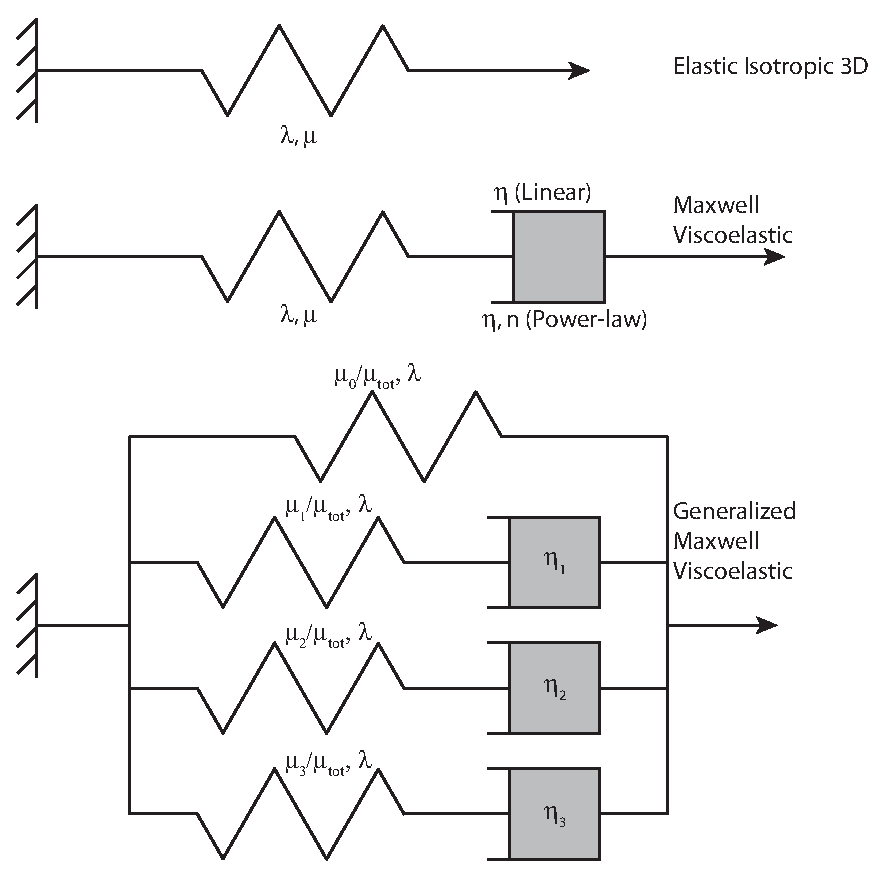
\includegraphics[scale=0.75]{materials/figs/pylith-materials}\caption{\label{fig:material:models}Spring-dashpot 1D representations of the
available 3D elastic and 2D/3D viscoelastic material models for PyLith.
The top model is a linear elastic model, the middle model is a Maxwell
model, and the bottom model is a generalized Maxwell model. For the
generalized Maxwell model, $\lambda$ and $\mu_{tot}$ are specified
for the entire model, and then the ratio $\mu_{i}/\mu_{tot}$ is specified
for each Maxwell model. For the power-law model, the linear dashpot
in the Maxwell model is replaced by a nonlinear dashpot obeying a
power-law.}
\end{figure}

\par\end{center}


\subsection{Definitions}

In the following sections, we use a combination of vector and index
notation (our notation conventions are shown in Table \vref{tab:notation}).
When using index notation, we use the common convention where repeated
indices indicate summation over the range of the index. We also make
frequent use of the scalar inner product. The scalar inner product
of two second-order tensors may be written
\begin{gather}
\underline{a}\cdot\underline{b}=a_{ij}b_{ij}\,.\label{eq:14}
\end{gather}
Although the general constitutive relations are formulated in terms
of the stress and strain, we frequently make use of the deviatoric
stress and strain in our formulation. We first define the mean stress,
$P$, and mean strain, $\theta$:
\begin{gather}
P=\frac{\sigma_{ii}}{3}\,,\,\,\,\,\theta=\frac{\epsilon_{ii}}{3}\,,\label{eq:15}
\end{gather}
where the $\sigma_{ii}$ and $\epsilon_{ii}$ represent the trace
of the stress and strain tensors, respectively. We then define the
deviatoric components of stress and strain as
\begin{gather}
S_{ij}=\sigma_{ij}-P\delta_{ij}\,,\,\,\,\, e_{ij}=\epsilon_{ij}-\theta\delta_{ij}\,,\label{eq:16}
\end{gather}
where $\delta_{ij}$ is the Kronecker delta. Using the deviatoric
components, we define the effective stress, $\overline{\sigma}$,
the second deviatoric stress invariant, $J_{2}^{\prime}$, the effective
deviatoric strain, $\overline{e}$, and the second deviatoric strain
invariant, $L_{2}^{\prime}$, as
\begin{gather}
\overline{\sigma}=\sqrt{\frac{3}{2}\underline{S}\cdot\underline{S}}\,\,\nonumber \\
J_{2}^{\prime}=\frac{1}{2}\underline{S}\cdot\underline{S}\,.\label{eq:17}\\
\overline{e}=\sqrt{\frac{2}{3}\underline{e}\cdot\underline{e}}\,\,\nonumber \\
L_{2}^{\prime}=\frac{1}{2}\underline{e}\cdot\underline{e}\,\,\nonumber 
\end{gather}
Due to the symmetry of the stress and strain tensors, it is sometimes
convenient to represent them as vectors:
\begin{gather}
\overrightarrow{\sigma^{T}}=\left[\begin{array}{cccccc}
\sigma_{11} & \sigma_{22} & \sigma_{33} & \sigma_{12} & \sigma_{23} & \sigma_{31}\end{array}\right]\label{eq:18}\\
\overrightarrow{\epsilon^{T}}=\left[\begin{array}{cccccc}
\epsilon_{11} & \epsilon_{22} & \epsilon_{33} & \epsilon_{12} & \epsilon_{23} & \epsilon_{31}\end{array}\right]\:.\nonumber 
\end{gather}
Note that when taking the scalar inner product of two tensors represented
as vectors, it is necessary to double the products representing off-diagonal
terms.

For quantities evaluated over a specific time period, we represent
the initial time as a pvrefixed subscript and the end time as a pvrefixed
superscript. In cases where the initial time does not appear, it is
understood to be $-\infty$.

\noindent \begin{center}
\begin{table}[H]
\noindent \centering{}\caption{\label{tab:notation}Mathematical notation used in this
section.}
\begin{tabular}{|c|c|c|}
\hline 
Index notation & Vector notation & Description\tabularnewline
\hline 
\hline 
$a_{i}$ & $\overrightarrow{a}$ & Vector field a\tabularnewline
\hline 
$a_{ij}$ & $\underline{a}$ & Second order tensor field a\tabularnewline
\hline 
\end{tabular}
\end{table}

\par\end{center}


\subsection{Linear Viscoelastic Models}

Linear viscoelastic models are obtained by various combinations of
a linear elastic spring and a linear viscous dashpot in series or
parallel. The simplest example is probably the linear Maxwell model,
which consists of a spring in series with a dashpot, as shown in Figure
\vref{fig:material:models}. For a one-dimensional model, the response
is given by
\begin{equation}
\frac{d\epsilon_{Total}}{dt}=\frac{d\epsilon_{D}}{dt}+\frac{d\epsilon_{S}}{dt}=\frac{\sigma}{\eta}+\frac{1}{E}\frac{d\sigma}{dt}\:,
\end{equation}
where $\epsilon_{Total}$ is the total strain, $\epsilon_{D}$ is
the strain in the dashpot, $\epsilon_{S}$ is the strain in the spring,
$\sigma$ is the stress, $\eta$ is the viscosity of the dashpot,
and $E$ is the spring constant. When a Maxwell material is subjected
to constant strain, the stresses relax exponentially with time. When
a Maxwell material is subjected to a constant stress, there is an
immediate elastic strain, corresponding to the response of the spring,
and a viscous strain that increases linearly with time. Since the
strain response is unbounded, the Maxwell model actually represents
a fluid.

Another simple model is the Kelvin-Voigt model, which consists of
a spring in parallel with a dashpot. In this case, the one-dimensional
response is given by
\begin{equation}
\sigma\left(t\right)=E\epsilon\left(t\right)+\eta\frac{d\epsilon\left(t\right)}{dt}\:.
\end{equation}
As opposed to the Maxwell model, which represents a fluid, the Kelvin-Voigt
model represents a solid undergoing reversible, viscoelastic strain.
If the material is subjected to a constant stress, it deforms at a
decreasing rate, gradually approaching the strain that would occur
for a purely elastic material. When the stress is released, the material
gradually relaxes back to its undeformed state.

The most general form of linear viscoelastic model is the generalized
Maxwell model, which consists of a spring in parallel with a number
of Maxwell models (see Figure \vref{fig:material:models}). Using this
model, it is possible to represent a number of simpler viscoelastic
models. For example, a simple Maxwell model is obtained by setting
the elastic constants of all springs to zero, with the exception of
the spring contained in the first Maxwell model ($\mu_{1}$). Similarly,
the Kelvin-Voigt model may be obtained by setting the elastic constants
$\mu_{2}=\mu_{3}=0$, and setting $\mu_{1}=\infty$ (or a very large
number).


\subsection{Formulation for Generalized Maxwell Models\label{sub:Formulation-for-Gen-Max}}

As described above, the generalized Maxwell viscoelastic model consists
of a number of Maxwell linear viscoelastic models in parallel with
a spring, as shown in Figure \vref{fig:material:models}. PyLith includes
the specific case of a spring in parallel with three Maxwell models.
As described in the previous paragraph, a number of common material
models may be obtained from this model by setting the shear moduli
of various springs to zero or infinity (or a large number), such as
the Maxwell model, the Kelvin model, and the standard linear solid.
We follow formulations similar to those used by Zienkiewicz and Taylor
\cite{Zienkiewicz:Taylor:2000} and Taylor \cite{Taylor:2003}. In
this formulation, we specify the total shear modulus of the model
($\mu_{tot}$) and Lame's constant ($\lambda$). We then provide the
fractional shear modulus for each Maxwell element spring in the model.
It is not necessary to specify the fractional modulus for $\mu_{0}$,
since this is obtained by subtracting the sum of the other ratios
from 1. Note that the sum of all these fractions must equal 1. We
use a similar formulation for our linear Maxwell viscoelastic model,
but in that case $\mu_{0}$ is always zero and we only use a single
Maxwell model. The parameters defining the standard Maxwell model
are shown in Table \vref{tab:linearMaxwell}, and those defining the
generalized Maxwell model are shown in Table \vref{tab:genMaxwell}.

As for all our viscoelastic models, the volumetric strain is completely
elastic, and the viscoelastic deformation may be expressed purely
in terms of the deviatoric components:
\begin{equation}
\underline{S}=2\mu_{tot}\left[\mu_{0}\underline{e}+\sum_{i=1}^{N}\mu_{i}\underline{q}^{i}-\underline{e}^{I}\right]+\underline{S}^{I}\,;\; P=3K\left(\theta-\theta^{I}\right)+P^{I}\,,\label{eq:19}
\end{equation}
where \textsl{K} is the bulk modulus, $N$ is the number of Maxwell
models, and the variable $\underline{q}^{i}$ follows the evolution
equations
\begin{equation}
\underline{\dot{q}}^{i}+\frac{1}{\tau_{i}}\underline{q}^{i}=\underline{\dot{e}}.\label{eq:20}
\end{equation}
The $\tau_{i}$ are the relaxation times for each Maxwell model:
\begin{equation}
\tau_{i}=\frac{\eta_{i}}{\mu_{tot}\mu_{i}}\:.\label{eq:21-1}
\end{equation}


An alternative to the differential equation form above is an integral
equation form expressed in terms of the relaxation modulus function.
This function is defined in terms of an idealized experiment in which,
at time labeled zero ($t=0$), a specimen is subjected to a constant
strain, $\underline{e}_{0}$, and the stress response, $\underline{S}\left(t\right)$,
is measured. For a linear material we obtain:
\begin{equation}
\underline{S}\left(t\right)=2\mu\left(t\right)\left(\underline{e}_{0}-\underline{e}^{I}\right)+\underline{S}^{I}\,,\label{eq:21}
\end{equation}
where $\mu\left(t\right)$ is the shear relaxation modulus function.
Using linearity and superposition for an arbitrary state of strain
yields an integral equation:
\begin{equation}
\underline{S}\left(t\right)=\intop_{-\infty}^{t}\mu\left(t-T\right)\underline{\dot{e}}\, dT\,.\label{eq:22}
\end{equation}
If we assume the modulus function in Prony series form we obtain
\begin{equation}
\mu\left(t\right)=\mu_{tot}\left(\mu_{0}+\sum_{i=1}^{N}\mu_{i}\exp\frac{-t}{\tau_{i}}\right)\,,\label{eq:23}
\end{equation}
where
\begin{equation}
\mu_{0}+\sum_{i=1}^{N}\mu_{i}=1\,.\label{eq:24}
\end{equation}
With the form in Equation \vref{eq:23}, the integral equation form
is identical to the differential equation form.

If we assume the material is undisturbed until a strain is suddenly
applied at time zero, we can divide the integral into
\begin{equation}
\intop_{-\infty}^{t}\left(\cdot\right)\, dT=\intop_{-\infty}^{0^{-}}\left(\cdot\right)\, dT+\intop_{0^{-}}^{0^{+}}\left(\cdot\right)\, dT+\intop_{0^{+}}^{t}\left(\cdot\right)\, dT\,.\label{eq:27}
\end{equation}
The first term is zero, the second term includes a jump term associated
with $\underline{e}_{0}$ at time zero, and the last term covers the
subsequent history of strain. Applying this separation to Equation
\vref{eq:22},
\begin{equation}
\underline{S}\left(t\right)=2\mu\left(t\right)\left(\underline{e}_{0}-\underline{e}^{I}\right)+\underline{S}^{I}+2\int_{0}^{t}\mu\left(t-T\right)\underline{\dot{e}}\left(T\right)\, dT\,,\label{eq:28}
\end{equation}
where we have left the sign off of the lower limit on the integral.

Substituting Equation \vref{eq:23} into \vref{eq:28}, we obtain
\begin{equation}
\underline{S}\left(t\right)=2\mu_{tot}\left\{ \mu_{0}\underline{e}\left(t\right)+\sum_{i=1}^{N}\left[\mu_{i}\exp\frac{-t}{\tau_{i}}\left(\underline{e}_{0}+\intop_{0}^{t}\exp\frac{t}{\tau_{i}}\underline{\dot{e}}\left(T\right)\, dT\right)\right]-\underline{e}^{I}\right\} +\underline{S}^{I}\,.\label{eq:29}
\end{equation}
We then split each integral into two ranges: from 0 to $t_{n}$, and
from $t_{n}$ to $t$, and define each integral as
\begin{equation}
\underline{i}_{i}^{1}\left(t\right)=\intop_{0}^{t}\exp\frac{T}{\tau_{i}}\underline{\dot{e}}\left(T\right)\, dT\,.\label{eq:30}
\end{equation}
The integral then becomes
\begin{equation}
\underline{i}_{i}^{1}\left(t\right)=\underline{i}_{i}^{1}\left(t_{n}\right)+\intop_{t_{n}}^{t}\exp\frac{T}{\tau_{i}}\underline{\dot{e}}\left(T\right)\, dT\,.\label{eq:31}
\end{equation}
Including the negative exponential multiplier:
\begin{equation}
\underline{h}_{i}^{1}\left(t\right)=\exp\frac{-t}{\tau_{i}}\underline{i}_{i}^{1}\,.\label{eq:32}
\end{equation}
Then
\begin{equation}
\underline{h}_{i}^{1}\left(t\right)=\exp\frac{-\Delta t}{\tau_{i}}\underline{h}_{i}^{1}\left(t_{n}\right)+\Delta\underline{h}_{i}\,,\label{eq:33}
\end{equation}
where
\begin{equation}
\Delta\underline{h}_{i}=\exp\frac{-t}{\tau_{i}}\intop_{t_{n}}^{t}\exp\frac{T}{\tau_{i}}\underline{\dot{e}}\left(T\right)\, dT\,.\label{eq:34}
\end{equation}
Approximating the strain rate as constant over each time step, the
solution may be found as
\begin{equation}
\Delta\underline{h}_{i}=\frac{\tau_{i}}{\Delta t}\left(1-\exp\frac{-\Delta t}{\tau_{i}}\right)\left(\underline{e}-\underline{e}_{n}\right)=\Delta h_{i}\left(\underline{e}-\underline{e}_{n}\right)\,.\label{eq:35}
\end{equation}
The approximation is singular for zero time steps, but a series expansion
may be used for small time-step sizes:
\begin{equation}
\Delta h_{i}\approx1-\frac{1}{2}\left(\frac{\Delta t}{\tau_{i}}\right)+\frac{1}{3!}\left(\frac{\Delta t}{\tau_{i}}\right)^{2}-\frac{1}{4!}\left(\frac{\Delta t}{\tau_{i}}\right)^{3}+\cdots\,.\label{eq:36}
\end{equation}
This converges with only a few terms. With this formulation, the constitutive
relation now has the simple form:
\begin{equation}
\underline{S}\left(t\right)=2\mu_{tot}\left(\mu_{0}\underline{e}\left(t\right)+\sum_{i=1}^{N}\mu_{i}\underline{h}_{i}^{1}\left(t\right)-\underline{e}^{I}\right)+\underline{S}^{I}\,.\label{eq:37}
\end{equation}


We need to compute the tangent constitutive matrix when forming the
stiffness matrix. In addition to the volumetric contribution to the
tangent constitutive matrix, we require the deviatoric part:
\begin{equation}
\frac{\partial\underline{S}}{\partial\underline{\epsilon}}=\frac{\partial\underline{S}}{\partial\underline{e}}\frac{\partial\underline{e}}{\partial\underline{\epsilon}}\,,\label{eq:38}
\end{equation}
where the second derivative on the right may be easily deduced from
Equation \vref{eq:16}. The other derivative is given by
\begin{equation}
\frac{\partial\underline{S}}{\partial\underline{e}}=2\mu_{tot}\left[\mu_{0}\underline{I}+\sum_{i=1}^{N}\mu_{i}\frac{\partial\underline{h}_{i}^{1}}{\partial\underline{e}}\right]\,,\label{eq:39}
\end{equation}
where $\underline{I}$ is the identity matrix. From Equations \vref{eq:33}
through \vref{eq:35}, the derivative inside the brackets is
\begin{equation}
\frac{\partial\underline{h}_{i}^{1}}{\partial\underline{e}}=\Delta h_{i}\left(\Delta t\right)\underline{I}\,.\label{eq:40}
\end{equation}
The complete deviatoric tangent relation is then
\begin{equation}
\frac{\partial\underline{S}}{\partial\underline{\epsilon}}=2\mu_{tot}\left[\mu_{0}+\sum_{i=1}^{N}\mu_{i}\Delta h_{i}\left(\Delta t\right)\right]\frac{\partial\underline{e}}{\partial\underline{\epsilon}}\,.\label{eq:41}
\end{equation}


We use this formulation for both our Maxwell and generalized Maxwell
viscoelastic models. For the Maxwell model, $\mu_{0}=0$ and $N=1$.
For the generalized Maxwell model, $N=3.$ The stable time step is
equal to 1/5 of the minimum relaxation time for all of the Maxwell
models (equation \vref{eq:21-1}).

\noindent \begin{center}
\begin{table}[H]
\noindent \centering{}\caption{\label{tab:linearMaxwell}Values in spatial databases for the linear
Maxwell viscoelastic material constitutive model.}
\begin{tabular}{|l|l|l|}
\hline 
\textbf{Spatial database} & \textbf{Value} & \textbf{Description}\tabularnewline
\hline 
\hline 
\multirow{4}{*}{\texttt{db\_properties}} & \texttt{vp} & Compressional wave speed, $v_{p}$\tabularnewline
\cline{2-3} 
 & \texttt{vs} & Shear wave speed, $v_{s}$\tabularnewline
\cline{2-3} 
 & \texttt{density} & Density, $\rho$\tabularnewline
\cline{2-3} 
 & \texttt{viscosity} & Viscosity, $\eta$\tabularnewline
\hline 
\texttt{db\_initial\_stress} & \texttt{stress-xx, }etc. & Initial stress components\tabularnewline
\hline 
\texttt{db\_initial\_strain} & \texttt{total-strain-xx, }etc. & Initial strain components\tabularnewline
\hline 
\multirow{2}{*}{\texttt{db\_initial\_state}} & \texttt{viscous-strain-xx, }etc. & Initial viscous strain components\tabularnewline
\cline{2-3} 
 & \texttt{stress-zz-initial} & Initial out-of-plane stress (2D only)\tabularnewline
\hline 
\end{tabular}
\end{table}

\par\end{center}

\noindent \begin{center}
\begin{table}[H]
\noindent \centering{}\caption{\label{tab:genMaxwell}Values in spatial database used as parameters
in the generalized linear Maxwell viscoelastic material constitutive
model.}
\begin{tabular}{|l|l|l|}
\hline 
\textbf{Spatial database} & \textbf{Value} & \textbf{Description}\tabularnewline
\hline 
\hline 
\multirow{9}{*}{\texttt{db\_properties}} & \texttt{vp} & Compressional wave speed, $v_{p}$\tabularnewline
\cline{2-3} 
 & \texttt{vs} & Shear wave speed, $v_{s}$\tabularnewline
\cline{2-3} 
 & \texttt{density} & Density, $\rho$\tabularnewline
\cline{2-3} 
 & \texttt{shear-ratio-1} & Shear ratio for Maxwell model 1, $\mu_{1}/\mu_{tot}$\tabularnewline
\cline{2-3} 
 & \texttt{shear-ratio-2} & Shear ratio for Maxwell model 2, $\mu_{2}/\mu_{tot}$\tabularnewline
\cline{2-3} 
 & \texttt{shear-ratio-3} & Shear ratio for Maxwell model 3, $\mu_{3}/\mu_{tot}$\tabularnewline
\cline{2-3} 
 & \texttt{viscosity-1} & Viscosity for Maxwell model 1, $\eta_{1}$\tabularnewline
\cline{2-3} 
 & \texttt{viscosity-2} & Viscosity for Maxwell model 2, $\eta_{2}$\tabularnewline
\cline{2-3} 
 & \texttt{viscosity-3} & Viscosity for Maxwell model 3, $\eta_{3}$\tabularnewline
\hline 
\texttt{db\_initial\_stress} & \texttt{stress-xx, }etc. & Initial stress components\tabularnewline
\hline 
\texttt{db\_initial\_strain} & \texttt{total-strain-xx, }etc. & Initial strain components\tabularnewline
\hline 
\multirow{4}{*}{\texttt{db\_initial\_state}} & \texttt{viscous-strain-1-xx, }etc. & Initial viscous strain components for Maxwell model 1\tabularnewline
\cline{2-3} 
 & \texttt{viscous-strain-2-xx, }etc. & Initial viscous strain components for Maxwell model 2\tabularnewline
\cline{2-3} 
 & \texttt{viscous-strain-3-xx, }etc. & Initial viscous strain components for Maxwell model 3\tabularnewline
\cline{2-3} 
 & \texttt{stress-zz-initial} & Initial out-of-plane stress (2D only)\tabularnewline
\hline 
\end{tabular}
\end{table}

\par\end{center}


\subsection{\label{sub:Effective-Stress-Formulations-Viscoelastic}Effective
Stress Formulations for Viscoelastic Materials}

As an alternative to the approach outlined above, an effective stress
function formulation \cite{Kojic:Bathe:1987} may be employed for
both a linear Maxwell model and a power-law Maxwell model. Note that
this formulation is not presently employed for linear viscoelastic
models (see Appendix \vref{cha:materials:alternative:formulations}), but it
is used for power-law viscoelastic materials. For the viscoelastic
materials considered here, the viscous volumetric strains are zero
(incompressible flow), and it is convenient to separate the general
stress-strain relationship at time $t+\Delta t$ into deviatoric and
volumetric parts:
\begin{gather}
\phantom{}{}^{t+\Delta t}\underline{S}=\frac{E}{1+\nu}\left(^{t+\Delta t}\underline{e}-\phantom{}^{t+\Delta t}\underline{e}^{C}-\underline{e}^{I}\right)+\underline{S}^{I}=\frac{1}{a_{E}}\left(^{t+\Delta t}\underline{e}-\phantom{}^{t+\Delta t}\underline{e}^{C}-\underline{e}^{I}\right)\label{eq:42}\\
^{t+\Delta t}P=\frac{E}{1-2\nu}\left(^{t+\Delta t}\theta-\theta^{I}\right)+P^{I}=\frac{1}{a_{m}}\left(^{t+\Delta t}\theta-\theta^{I}\right)\:,\nonumber 
\end{gather}
where $^{t+\Delta t}\underline{e}$ is the total deviatoric strain,
$^{t+\Delta t}\underline{e}^{C}$ is the total viscous strain, $\underline{e}^{I}$
is the initial deviatoric strain, $^{t+\Delta t}P$ is the pressure,
$^{t+\Delta t}\theta$ is the mean strain evaluated at time $t+\Delta t$
, and $\theta^{I}$ is the initial mean strain. The initial deviatoric
stress and initial pressure are given by $\underline{S}^{I}$ and
$P^{I}$, respectively. The topmost equation in Equation \vref{eq:42}
may also be written as
\begin{gather}
^{t+\Delta t}\underline{S}=\frac{1}{a_{E}}(^{t+\Delta t}\underline{e}^{\prime}-\underline{\Delta e}^{C})+\underline{S}^{I}\,,\label{eq:43}
\end{gather}
where
\begin{gather}
^{t+\Delta t}\underline{e}^{\prime}=\phantom{}^{t+\Delta t}\underline{e}-\phantom{}^{t}\underline{e}^{C}-\underline{e}^{I}\,\,,\,\,\,\underline{\Delta e}^{C}=\phantom{}^{t+\Delta t}\underline{e}^{C}-\phantom{}^{t}\underline{e}^{C}\,.\label{eq:44}
\end{gather}
The creep strain increment is approximated using
\begin{gather}
\underline{\Delta e}^{C}=\Delta t\phantom{}^{\tau}\gamma\phantom{}^{\tau}\underline{S}\,,\label{eq:45}
\end{gather}
where, using the $\alpha$-method of time integration,
\begin{gather}
^{\tau}\underline{S}=(1-\alpha)_{I}^{t}\underline{S}+\alpha\phantom{}_{I}^{t+\Delta t}\underline{S}+\underline{S}^{I}=(1-\alpha)^{t}\underline{S}+\alpha\phantom{}^{t+\Delta t}\underline{S}\,\,,\label{eq:46}
\end{gather}
and
\begin{gather}
^{\tau}\gamma=\frac{3\Delta\overline{e}^{C}}{2\Delta t\phantom{}^{\tau}\overline{\sigma}}\,\,,\label{eq:47}
\end{gather}
where
\begin{gather}
\Delta\overline{e}^{C}=\sqrt{\frac{2}{3}\underline{\Delta e}^{C}\cdot\underline{\Delta e}^{C}}\label{eq:48}
\end{gather}
and
\begin{gather}
^{\tau}\overline{\sigma}=(1-\alpha)_{I}^{t}\overline{\sigma}+\alpha\phantom{}_{I}^{t+\Delta t}\overline{\sigma}+\overline{\sigma}^{I}=\sqrt{3\phantom{}^{\tau}J_{2}^{\prime}}\,\,.\label{eq:49}
\end{gather}


To form the global stiffness matrix, it is necessary to provide a
relationship for the viscoelastic tangent material matrix relating
stress and strain. If we use vectors composed of the stresses and
tensor strains, this relationship is
\begin{gather}
\underline{C}^{VE}=\frac{\partial\phantom{}^{t+\Delta t}\overrightarrow{\sigma}}{\partial\phantom{}^{t+\Delta t}\overrightarrow{\epsilon}}\,\,.\label{eq:55}
\end{gather}
In terms of the vectors, we have
\begin{gather}
^{t+\Delta t}\sigma_{i}=\phantom{}^{t+\Delta t}S_{i}+\phantom{}^{t+\Delta t}P\,\,;\,\,\, i=1,2,3\label{eq:56}\\
^{t+\Delta t}\sigma_{i}=\phantom{}^{t+\Delta t}S_{i}\,;\,\,\,\,\,\,\,\,\,\,\,\,\,\,\,\,\,\,\,\,\,\,\,\,\,\,\,\,\,\,\, i=4,5,6\nonumber 
\end{gather}
Thevrefore,
\begin{gather}
C_{ij}^{VE}=C_{ij}^{\prime}+\frac{1}{3a_{m}}\,;\,\,1\leq i,j\leq3\,\,.\label{eq:57}\\
C_{ij}^{VE}=C_{ij}^{\prime}\,;\,\,\,\,\,\,\,\,\,\,\,\,\,\,\,\,\,\,\,\,\,\,\,\,\,\,\,\,\,\,\,\,\,\,\,\textrm{otherwise}\nonumber 
\end{gather}
Using the chain rule,
\begin{gather}
C_{ij}^{\prime}=\frac{\partial\phantom{}^{t+\Delta t}S_{i}}{\partial\phantom{}^{t+\Delta t}\epsilon_{j}}=\frac{\partial\phantom{}^{t+\Delta t}S_{i}}{\partial\phantom{}^{t+\Delta t}e_{k}^{\prime}}\frac{\partial\phantom{}^{t+\Delta t}e_{k}^{\prime}}{\partial\phantom{}^{t+\Delta t}e_{l}}\frac{\partial\phantom{}^{t+\Delta t}e_{l}}{\partial\phantom{}^{t+\Delta t}\epsilon_{j}}\,\,.\label{eq:58}
\end{gather}
From Equation \vref{eq:44}, we obtain
\begin{gather}
\frac{\partial\phantom{}^{t+\Delta t}e_{k}^{\prime}}{\partial\phantom{}^{t+\Delta t}e_{l}}=\delta_{kl}\,\,,\label{eq:59}
\end{gather}
and from Equation \vref{eq:16}:
\begin{gather}
\frac{\partial\phantom{}^{t+\Delta t}e_{l}}{\partial\phantom{}^{t+\Delta t}\epsilon_{j}}=\frac{1}{3}\left[\begin{array}{ccc}
2 & -1 & -1\\
-1 & 2 & -1\\
-1 & -1 & 2
\end{array}\right];\,\,1\leq l,j\leq3\label{eq:60}\\
\frac{\partial\phantom{}^{t+\Delta t}e_{l}}{\partial\phantom{}^{t+\Delta t}\epsilon_{j}}=\delta_{lj}\,\,;\,\,\,\,\,\,\,\,\,\,\,\,\,\,\,\,\,\,\,\,\,\,\,\,\,\,\,\,\,\,\,\,\,\,\,\,\,\,\,\,\,\,\,\,\textrm{otherwise.}\nonumber 
\end{gather}
The first term of Equation \vref{eq:58} depends on the particular
constitutive relationship, and the complete tangent matrix may then
be obtained from Equation \vref{eq:57}.


\subsubsection{Power-Law Maxwell Viscoelastic Material\label{sub:Power-Law-Maxwell-Viscoelastic}}

Laboratory results on rock rheology are typically performed using
a triaxial experiment, and the creep data are fit to a power-law equation
of the form (e.g., \cite{Kirby:Kronenberg:1987}):
\begin{equation}
\dot{\epsilon}_{11}^{C}=A_{E}\exp\left(\frac{-Q}{RT}\right)\left(\sigma_{1}-\sigma_{3}\right)^{n}=A_{E}\exp\left(\frac{-Q}{RT}\right)\sigma_{d}^{n}\:,\label{eq:64}
\end{equation}
where $\dot{\epsilon}_{11}^{C}$ is the strain rate in the direction
of the maximum principal stress $\left(\sigma_{1}\right)$, $A_{E}$
is the experimentally-derived pre-exponential constant, $Q$ is the
activation enthalpy, $R$ is the universal gas constant, $T$ is the
absolute temperature, $n$ is the power-law exponent, $\sigma_{3}\:\left(=\sigma_{2}\right)$
is equal to the confining pressure, and $\sigma_{d}$ is the differential
stress. To properly formulate the flow law, it must be generalized
so that the results are not influenced by the experiment type or the
choice of coordinate systems (e.g., \cite{Paterson:1994}). The flow
law may then be generalized in terms of the deviatoric stress and
strain rate invariants:
\begin{equation}
\sqrt{\dot{L}_{2}^{\prime C}}=A_{M}\exp\left(\frac{-Q}{RT}\right)\sqrt{J_{2}^{\prime}}^{n}\:,\label{eq:65}
\end{equation}
where $A_{M}$ is now a pre-exponential constant used in the formulation
for modeling. In practice, it is necessary to compute each strain
rate component using the flow law. This is accomplished using:
\begin{equation}
\dot{e}_{ij}^{C}=A_{M}\exp\left(\frac{-Q}{RT}\right)\sqrt{J_{2}^{\prime}}^{n-1}S_{ij}\:.\label{eq:66}
\end{equation}
Note that Equations \vref{eq:65} and \vref{eq:66} are consistent,
since Equation \vref{eq:65} may be obtained from Equation \vref{eq:66}
by taking the scalar inner product of both sides, multiplying by 1/2,
and taking the square root.

In a triaxial experiment with confining pressure $P_{c}$, we have
\begin{gather}
\sigma_{2}=\sigma_{3}=P_{c}\nonumber \\
\sigma_{1}=\sigma_{1}^{app}\label{eq:67}\\
P=\frac{\sigma_{1}+2P_{c}}{3}\:,\nonumber 
\end{gather}
where $\sigma_{1}^{app}$ is the applied load. The deviatoric stresses
are then:
\begin{gather}
S_{1}=\frac{2}{3}\left(\sigma_{1}-P_{c}\right)\nonumber \\
S_{2}=S_{3}=-\frac{1}{3}\left(\sigma_{1}-P_{c}\right)\:.\label{eq:68}
\end{gather}
This gives
\begin{gather}
S_{1}=\frac{2}{3}\left(\sigma_{1}-\sigma_{3}\right)=\frac{2}{3}\sigma_{d}\nonumber \\
S_{2}=S_{3}=-\frac{1}{3}\left(\sigma_{1}-\sigma_{3}\right)=-\frac{1}{3}\sigma_{d}\:.\label{eq:69}
\end{gather}
In terms of the second deviatoric stress invariant, we then have
\begin{equation}
\sqrt{J_{2}^{\prime}}=\frac{\sigma_{d}}{\sqrt{3}}\:.\label{eq:70}
\end{equation}


Under the assumption that the creep measured in the laboratory experiments
is incompressible, we have
\begin{gather}
\dot{e}_{11}^{C}=\dot{\epsilon}_{11}\nonumber \\
\dot{e}_{22}^{C}=\dot{e}_{33}^{C}=-\frac{1}{2}\dot{\epsilon}_{11}\:.\label{eq:71}
\end{gather}
In terms of the second deviatoric strain rate invariant we then have
\begin{equation}
\sqrt{\dot{L}_{2}^{\prime C}}=\frac{\sqrt{3}}{2}\dot{\epsilon}_{11}\:.\label{eq:72}
\end{equation}
Substituting Equations \vref{eq:70} and \vref{eq:72} into Equation
\vref{eq:64}, we obtain
\begin{equation}
\sqrt{\dot{L}_{2}^{\prime C}}=A_{E}\frac{\sqrt{3}^{n+1}}{2}\exp\left(\frac{-Q}{RT}\right)\sqrt{J_{2}^{\prime}}^{n}\:,\label{eq:73}
\end{equation}
and thevrefore,
\begin{equation}
A_{M}=\frac{\sqrt{3}^{n+1}}{2}A_{E}\:.\label{eq:74}
\end{equation}
When the exponential factor is included, we define a new parameter:

\begin{equation}
A_{T}=A_{M}\exp\left(\frac{-Q}{RT}\right)=\frac{\sqrt{3}^{n+1}}{2}A_{E}\exp\left(\frac{-Q}{RT}\right)\:.\label{eq:75}
\end{equation}


There is a problem with the usage of parameters $A_{E}$, $A_{M}$,
and $A_{T}$. Since the dimensions of these parameters are dependent
on the value of the power-law exponent, they are not really constants.
In addition to being logically inconsistent, this presents problems
when specifying parameters for PyLith, since the power-law exponent
must be known before the units can be determined. An alternative way
of writing the flow rule is (e.g., \cite{Prentice:1968}): 
\begin{equation}
\frac{\sqrt{\dot{L}_{2}^{\prime C}}}{\dot{e}_{0}}=\left(\frac{\sqrt{J_{2}^{\prime}}}{S_{0}}\right)^{n},\label{eq:76}
\end{equation}
where $\dot{e}_{0}$ and $S_{0}$ are vreference values for the strain
rate and deviatoric stress. This means that
\begin{equation}
\frac{\dot{e}_{0}}{S_{0}^{n}}=A_{T}\:.\label{eq:77}
\end{equation}
Users must thevrefore specify three parameters for a power-law material.
The properties \texttt{vreference-strain-rate}, \texttt{vreference-stress},
and \texttt{power-law-exponent} in Table \vref{tab:powerLaw} vrefer
to $\dot{e}_{0}$, $S_{0}$, and $n$, respectively. To specify the
power-law properties for PyLith using laboratory results, the user
must first compute $A_{T}$ using Equation \vref{eq:75}. Then, values
for $\dot{e}_{0}$ and $S_{0}$ must be provided. The simplest method
is probably to assume a reasonable value for the vreference strain
rate, and then compute $S_{0}$ as
\begin{equation}
S_{0}=\left(\frac{\dot{e}_{0}}{A_{T}}\right)^{\frac{1}{n}}\:.\label{eq:78}
\end{equation}


A utility code (\texttt{powerlaw\_gendb.py}) is provided to convert
laboratory results to the properties used by PyLith. To use the code,
users must specify the spatial variation of $A_{E}$, $Q$, $n$,
and $T$. An additional parameter is given to define the units of
$A_{E}$. The user then specifies either a vreference stress or a vreference
strain rate, and a database suitable for PyLith is generated. This
utility is described more fully in Section \vref{sub:Tutorial-Step08-Power-law}.

The flow law in component form is 
\begin{equation}
\dot{e}_{ij}^{C}=\frac{\dot{e}_{0}\sqrt{J_{2}^{\prime}}^{n-1}S_{ij}}{S_{0}^{n}}\:,\label{eq:79}
\end{equation}
and the creep strain increment is approximated as
\begin{gather}
\underline{\Delta e}^{C}\approx\frac{\Delta t\dot{e}_{0}\sqrt{^{\tau}J_{2}^{\prime}}^{n-1}\,^{\tau}\underline{S}}{S_{0}^{n}}=\frac{\Delta t\dot{e}_{0}\phantom{}^{\tau}\overline{\sigma}^{n-1}\,^{\tau}\underline{S}}{\sqrt{3}S_{0}^{n}}\,.\label{eq:80}
\end{gather}
 Thevrefore,
\begin{gather}
\Delta\bar{e}^{C}\approx\frac{2\Delta t\dot{e}_{0}\sqrt{^{\tau}J_{2}^{\prime}}^{n}}{\sqrt{3}S_{0}^{n}}=\frac{2\Delta t\dot{e}_{0}\phantom{}^{\tau}\overline{\sigma}^{n}}{\sqrt{3}^{n+1}S_{0}^{n}}\,,\,\textrm{and}\,^{\tau}\gamma=\frac{\dot{e}_{0}\sqrt{^{\tau}J_{2}^{\prime}}^{n-1}}{S_{0}^{n}}\,.\label{eq:81}
\end{gather}
substituting Equations \vref{eq:46}, \vref{eq:80}, and \vref{eq:81}
into \vref{eq:43}, we obtain:
\begin{gather}
^{t+\Delta t}\underline{S}=\frac{1}{a_{E}}\left\{ ^{t+\Delta t}\underline{e}^{\prime}-\Delta t\phantom{}^{\tau}\gamma\left[\left(1-\alpha\right)^{t}\underline{S}+\alpha{}^{t+\Delta t}\underline{S}\right]\right\} +\underline{S}^{I}\,,\label{eq:82}
\end{gather}
which may be rewritten:
\begin{gather}
^{t+\Delta t}\underline{S}\left(a_{E}+\alpha\Delta t\phantom{}^{\tau}\gamma\right)={}^{t+\Delta t}\underline{e}^{\prime}-\Delta t\phantom{}^{\tau}\gamma\left(1-\alpha\right)^{t}\underline{S}+a_{E}\underline{S}^{I}\,.\label{eq:83}
\end{gather}
Taking the scalar inner product of both sides we obtain:
\begin{gather}
a^{2}\,\,{}^{t+\Delta t}J_{2}^{\prime}-b+c\phantom{}^{\tau}\gamma-d^{2}\,^{\tau}\gamma^{2}=F=0\,,\label{eq:84}
\end{gather}
where
\begin{gather}
a=a_{E}+\alpha\Delta t\phantom{}^{\tau}\gamma\,\,\nonumber \\
b=\frac{1}{2}{}^{t+\Delta t}\underline{e}^{\prime}\cdot{}^{t+\Delta t}\underline{e}^{\prime}+a_{E}{}^{t+\Delta t}\underline{e}^{\prime}\cdot\underline{S}^{I}+a_{E}^{2}\,^{I}J_{2}^{\prime}\,.\label{eq:85}\\
c=\Delta t\left(1-\alpha\right){}^{t+\Delta t}\underline{e}^{\prime}\cdot^{t}\underline{S}+\Delta t\left(1-\alpha\right)a_{E}\,^{t}\underline{S}\cdot\underline{S}^{I}\,\,\nonumber \\
d=\Delta t\left(1-\alpha\right)\sqrt{^{t}J_{2}^{\prime}}\,\,\nonumber 
\end{gather}
Equation \vref{eq:84} is a function of a single unknown -- the square
root of the second deviatoric stress invariant at time $t+\Delta t$
-- and may be solved by bisection or by Newton's method. Once this
parameter has been found, the deviatoric stresses for the current
time step may be found from Equations \vref{eq:49}, \vref{eq:81},
and \vref{eq:82}, and the total stresses may be found by combining
the deviatoric and volumetric components from Equation \vref{eq:42}.

Once the stresses are computed for the current time step, we can compute
the relaxation time (used in computing the stable time step) by first
computing the effective viscous strain rate from Equation \vref{eq:79}:
\begin{equation}
\dot{\bar{e}}^{C}=\frac{2\dot{e}_{0}\left(\frac{\bar{\sigma}}{\sqrt{3}}\right)^{n}}{\sqrt{3}S_{0}^{n}}\:.
\end{equation}
Similarly, the effective elastic strain is computed as:
\begin{equation}
\bar{e}^{E}=\frac{\bar{\sigma}}{3\mu}\:.
\end{equation}
The relaxation time is then the ratio between these two:
\begin{equation}
\tau=\frac{\bar{e}^{E}}{\bar{\dot{e}}^{C}}=\left(\frac{S_{0}}{\sqrt{J_{2}^{\prime}}}\right)^{n-1}\frac{S_{0}}{6\mu\dot{e}_{0}}\:.\label{eq:86-1}
\end{equation}
The stable time step returned by PyLith is 1/5 of the value computed
from Equation \vref{eq:86-1}.

To compute the tangent stress-strain relation, we need to compute
the first term in Equation \vref{eq:58}. We begin by rewriting Equation
\vref{eq:83} as
\begin{gather}
F=^{t+\Delta t}S_{i}\left(a_{E}+\alpha\Delta t\phantom{}^{\tau}\gamma\right)-\phantom{}^{t+\Delta t}e_{i}^{\prime}+\Delta t\phantom{}^{\tau}\gamma\left(1-\alpha\right)^{t}S_{i}-a_{E}S_{i}^{I}=0\:.\label{eq:86}
\end{gather}
The derivative of this function with respect to $^{t+\Delta t}e_{k}^{\prime\prime}$
is
\begin{gather}
\frac{\partial F}{\partial\phantom{}^{t+\Delta t}e_{k}^{\prime}}=-\delta_{ik}\:,\label{eq:87}
\end{gather}
and the derivative with respect to $^{t+\Delta t}S_{i}$ is
\begin{gather}
\frac{\partial F}{\partial\phantom{}^{t+\Delta t}S_{i}}=a_{E}+\alpha\Delta t\phantom{}^{\tau}\gamma+\frac{\partial\phantom{}^{\tau}\gamma}{\partial\phantom{}^{t+\Delta t}S_{i}}\Delta t\left[\alpha\phantom{}^{t+\Delta t}S_{i}+\left(1-\alpha\right)^{t}S_{i}\right]\:.\label{eq:88}
\end{gather}
From Equation \vref{eq:81} and Equation \vref{eq:49},
\begin{gather}
^{\tau}\gamma=\frac{\dot{e}_{0}}{S_{0}^{n}}\left[\alpha\sqrt{^{t+\Delta t}J_{2}^{\prime}}+\left(1-\alpha\right)\sqrt{^{t}J_{2}^{\prime}}\right]^{n-1}\:.\label{eq:89}
\end{gather}
Then
\begin{gather}
\frac{\partial\phantom{}^{\tau}\gamma}{\partial{}^{t+\Delta t}S_{i}}=\frac{\partial\phantom{}^{\tau}\gamma}{\partial\sqrt{^{t+\Delta t}J_{2}^{\prime}}}\frac{\partial\sqrt{^{t+\Delta t}J_{2}^{\prime}}}{\partial\phantom{}^{t+\Delta t}S_{l}}\label{eq:90}\\
=\frac{\dot{e}_{0}\alpha\left(n-1\right)\sqrt{^{\tau}J_{2}^{\prime}}^{n-2}{}^{t+\Delta t}T_{i}}{2S_{0}^{n}}\,,\nonumber 
\end{gather}
where
\begin{gather}
^{t+\Delta t}T_{i}=\phantom{}^{t+\Delta t}S_{i}\:;\:\:1\leq i\leq3\label{eq:91}\\
^{t+\Delta t}T_{i}=2\phantom{}^{t+\Delta t}S_{i}\:;\:\:\textrm{otherwise.}\nonumber 
\end{gather}
Then using Equations \vref{eq:87}, \vref{eq:88}, \vref{eq:90}, and
the quotient rule for derivatives of an implicit function,
\begin{gather}
\frac{\partial\phantom{}^{t+\Delta t}S_{i}}{\partial{}^{t+\Delta t}e_{k}^{\prime}}=\frac{\delta_{ik}}{a_{E}+\alpha\Delta t\left[^{\tau}\gamma+\frac{\dot{e}_{0}{}^{\tau}S_{i}\left(n-1\right){}^{t+\Delta t}T_{i}\sqrt{^{\tau}J_{2}^{\prime}}^{n-2}}{2\sqrt{^{t+\Delta t}J_{2}^{\prime}}S_{0}^{n}}\right]}\,.\label{eq:92}
\end{gather}
Note that for a linear material $\left(n=1\right)$, this equation
is identical to the linear formulation in Section \vref{sub:Effective-Stress-Formulation-Maxwell}
(making the appropriate substitution for $^{\tau}\gamma$). Then,
using Equations \vref{eq:57} through \vref{eq:60},
\begin{gather}
C_{ij}^{VE}=\frac{1}{3a_{m}}\left[\begin{array}{cccccc}
1 & 1 & 1 & 0 & 0 & 0\\
1 & 1 & 1 & 0 & 0 & 0\\
1 & 1 & 1 & 0 & 0 & 0\\
0 & 0 & 0 & 0 & 0 & 0\\
0 & 0 & 0 & 0 & 0 & 0\\
0 & 0 & 0 & 0 & 0 & 0
\end{array}\right]+\frac{1}{3}\frac{\partial{}^{t+\Delta t}S_{i}}{\partial{}^{t+\Delta t}e_{k}^{\prime}}\left[\begin{array}{cccccc}
2 & -1 & -1 & 0 & 0 & 0\\
-1 & 2 & -1 & 0 & 0 & 0\\
-1 & -1 & 2 & 0 & 0 & 0\\
0 & 0 & 0 & 3 & 0 & 0\\
0 & 0 & 0 & 0 & 3 & 0\\
0 & 0 & 0 & 0 & 0 & 3
\end{array}\right]\,.\label{eq:93}
\end{gather}
Note that if there are no deviatoric stresses at the beginning and
end of a time step (or if $\nicefrac{\dot{e}_{0}}{S_{0}^{n}}$ approaches
zero), Equations \vref{eq:92} and \vref{eq:93} reduce to the elastic
constitutive matrix, as expected.

To compute the zero of the effective stress function using Newton's
method, we require the derivative of Equation \vref{eq:84}, which
may be written:
\begin{gather}
\frac{\partial F}{\partial\sqrt{^{t+\Delta t}J_{2}^{\prime}}}=2a^{2}\sqrt{^{t+\Delta t}J_{2}^{\prime}}+\frac{\dot{e}_{0}\alpha\left(n-1\right)\sqrt{^{\tau}J_{2}^{\prime}}^{n-2}}{S_{0}^{n}}\left(2a\alpha\Delta t{}^{t+\Delta t}J_{2}^{\prime}+c-2d^{2}\,^{\tau}\gamma\right)\,.\label{eq:94}
\end{gather}


\noindent \begin{center}
\begin{table}[H]
\noindent \centering{}\caption{\label{tab:powerLaw}Values in spatial database used as parameters
in the nonlinear power-law viscoelastic material constitutive model.}
\begin{tabular}{|l|l|l|}
\hline 
\textbf{Spatial database} & \textbf{Value} & \textbf{Description}\tabularnewline
\hline 
\hline 
\multirow{6}{*}{\texttt{db\_properties}} & \texttt{vp} & Compressional wave speed, $v_{p}$\tabularnewline
\cline{2-3} 
 & \texttt{vs} & Shear wave speed, $v_{s}$\tabularnewline
\cline{2-3} 
 & \texttt{density} & Density, $\rho$\tabularnewline
\cline{2-3} 
 & \texttt{vreference-strain-rate} & Reference strain rate, $\dot{e}_{0}$\tabularnewline
\cline{2-3} 
 & \texttt{vreference-stress} & Reference stress, $S_{0}$\tabularnewline
\cline{2-3} 
 & \texttt{power-law-exponent} & Power-law exponent, $n$\tabularnewline
\hline 
\texttt{db\_initial\_stress} & \texttt{stress-xx, }etc. & Initial stress components\tabularnewline
\hline 
\texttt{db\_initial\_strain} & \texttt{total-strain-xx, }etc. & Initial strain components\tabularnewline
\hline 
\multirow{2}{*}{\texttt{db\_initial\_state}} & \texttt{viscous-strain-xx, }etc. & Initial viscous strain components\tabularnewline
\cline{2-3} 
 & \texttt{stress-zz-initial} & Initial out-of-plane stress (2D only)\tabularnewline
\hline 
\end{tabular}
\end{table}

\par\end{center}


\section{Elastoplastic Materials}

PyLith presently contains just a single elastoplastic material that
implements the Drucker-Prager yield criterion. Future releases of
PyLith may contain additional elastoplastic materials, such as Drucker-Prager
with hardening/softening.


\subsection{General Elastoplasticity Formulation}

The elastoplasticity formulation in PyLith is based on an additive
decomposition of the total strain into elastic and plastic parts:
\begin{equation}
d\epsilon_{ij}=d\epsilon_{ij}^{E}+d\epsilon_{ij}^{P}\:.\label{eq:95}
\end{equation}
The stress increment is then given by
\begin{equation}
d\sigma_{ij}=C_{ijrs}^{E}\left(d\epsilon_{rs}-d\epsilon_{rs}^{P}\right)\:,\label{eq:96}
\end{equation}
where $C_{ijrs}^{E}$ are the components of the elastic constitutive
tensor. To completely specify an elastoplastic problem, three components
are needed. We first require a yield condition, which specifies the
state of stress at which plastic flow initiates. This is generally
given in the form:
\begin{equation}
f\left(\underline{\sigma},k\right)=0\:,\label{eq:97}
\end{equation}
where \textit{k} is an internal state parameter. It is then necessary
to specify a flow rule, which describes the relationship between plastic
strain and stress. The flow rule is given in the form:
\begin{equation}
g\left(\underline{\sigma},k\right)=0\:.\label{eq:98}
\end{equation}
The plastic strain increment is then given as
\begin{equation}
d\epsilon_{ij}^{P}=d\lambda\frac{\partial g}{\partial\sigma_{ij}}\:,\label{eq:99}
\end{equation}
where $d\lambda$ is the scalar plastic multiplier. When the flow
rule is identical to the yield criterion ($f\equiv g$), the plasticity
is described as associated. Otherwise, it is non-associated. The final
component needed is a hardening hypothesis, which describes how the
yield condition and flow rule are modified during plastic flow. When
the yield condition and flow rule remain constant during plastic flow
(e.g., no hardening), the material is vreferred to as perfectly plastic.

To perform the solution, the yield condition (Equation \vref{eq:97})
is first evaluated under the assumption of elastic behavior. If $^{t+\Delta t}f<0$,
the material behavior is elastic and no plastic flow occurs. Otherwise,
the behavior is plastic and a plastic strain increment must be computed
to return the stress state to the yield envelope. This procedure is
known as an elastic predictor-plastic corrector algorithm.


\subsection{Drucker-Prager Elastoplastic Material}

PyLith includes an elastoplastic implementation of the Drucker-Prager
yield criterion \cite{Drucker:Prager:1952}. This criterion was originally
devised to model plastic deformation of soils, and it has also been
used to model rock deformation. It is intended to be a smooth approximation
of the Mohr-Coulomb yield criterion. The implementation used in PyLith
includes non-associated plastic flow, which allows control over the
unreasonable amounts of dilatation that are sometimes predicted by
the associated model. The model is described by the following yield
condition:
\begin{equation}
f\left(\underline{\sigma},k\right)=\alpha_{f}I_{1}+\sqrt{J_{2}^{\prime}}-\beta\:,\label{eq:100}
\end{equation}
and a flow rule given by:
\begin{equation}
g\left(\underline{\sigma},k\right)=\sqrt{J_{2}^{\prime}}+\alpha_{g}I_{1}\:.\label{eq:101}
\end{equation}


The yield surface represents a circular cone in principal stress space,
and the parameters can be related to the friction angle, $\phi$,
and the cohesion, $\bar{c}$, of the Mohr-Coulomb model. The yield
surface in Haigh-Westergaard space ($\zeta=\frac{1}{\sqrt{3}}I_{1},p=\sqrt{2J_{2}},\cos(3\theta)=\frac{3\sqrt{3}}{2}\frac{J_{3}}{J_{2}^{3/2}}$)
is
\begin{equation}
\left(\sqrt{3}\sin\left(\theta+\frac{\pi}{3}\right)-\sin\phi\cos\left(\theta+\frac{\pi}{3}\right)\right)p-\sqrt{2}\sin\phi\zeta=\sqrt{6}\overline{c}\cos\theta.\label{eq:drucker:prager:haigh:westergaard}
\end{equation}
The yield surface can be fit to the Mohr-Coulomb model in several
different ways. The yield surface can touch the outer apices ($\theta=\pi/3$)
of the Mohr-Coulomb model (inscribed version), the inner apices ($\theta=0$)
of the Mohr-Coulomb model (circumscribed version), or halfway between
the two ($\theta=pi/6,$middle version). Substituting these values
for $\theta$ into Equation (\vref{eq:drucker:prager:haigh:westergaard})
and casting it into the same form as Equation (\vref{eq:101}) yields
the values of $\alpha_{f}$, $\beta$, and $\alpha_{g}$ given in
Table \vref{tab:fit_mohr_coulomb}, where $\phi_{0}$ vrefers to the
initial friction angle. Similarly, the flow rule can be related to
the dilatation angle, $\psi$, of a Mohr-Coulomb model. It is also
possible for the Mohr-Coulomb parameters to be functions of the internal
state parameter, $k$. In PyLith, the fit to the Mohr-Coulomb yield
surface and flow rule is controlled by the \texttt{fit\_mohr\_coulomb}
property. 

\begin{table}
\caption{\label{tab:fit_mohr_coulomb}Options for fitting the Drucker-Prager
plastic parameters to a Mohr-Coulomb model using \texttt{fit\_mohr\_coulomb}.}


\centering{}%
\begin{tabular}{|c|c|c|c|}
\hline 
\textbf{Parameter Value} & $\alpha_{f}$ & $\beta$ & $\alpha_{g}$\tabularnewline
\hline 
\hline 
\texttt{inscribed} & $\frac{2\sin\phi\left(k\right)}{\sqrt{3}\left(3-\sin\phi\left(k\right)\right)}$ & $\frac{6\bar{c}\left(k\right)\cos\phi_{0}}{\sqrt{3}\left(3-\sin\phi_{0}\right)}$ & $\frac{2\sin\psi(k)}{\sqrt{3}\left(3-\sin\psi\left(k\right)\right)}$\tabularnewline
\hline 
\texttt{middle} & $\frac{\sin\phi\left(k\right)}{3}$ & $\bar{c}\left(k\right)\cos\left(\phi_{0}\right)$ & $\frac{\sin\psi\left(k\right)}{3}$\tabularnewline
\hline 
\texttt{circumscribed} & $\frac{2\sin\phi\left(k\right)}{\sqrt{3}\left(3+\sin\phi\left(k\right)\right)}$ & $\frac{6\bar{c}\left(k\right)\cos\phi_{0}}{\sqrt{3}\left(3+\sin\phi_{0}\right)}$ & $\frac{2\sin\psi(k)}{\sqrt{3}\left(3+\sin\psi\left(k\right)\right)}$\tabularnewline
\hline 
\end{tabular}
\end{table}


As for the viscoelastic models, it is convenient to separate the deformation
into deviatoric and volumetric parts:
\begin{gather}
^{t+\Delta t}S_{ij}=\frac{1}{a_{E}}\left(^{t+\Delta t}e_{ij}-\phantom{}^{t+\Delta t}e_{ij}^{P}-e_{ij}^{I}\right)+S_{ij}^{I}=\frac{1}{a_{E}}\left(^{t+\Delta t}e_{ij}^{\prime}-\Delta e_{ij}^{P}\right)+S_{ij}^{I}\label{eq:105}\\
^{t+\Delta t}P=\frac{1}{a_{m}}\left(^{t+\Delta t}\theta-\phantom{}^{t+\Delta t}\theta^{P}-\theta^{I}\right)+P^{I}=\frac{1}{a_{m}}\left(^{t+\Delta t}\theta^{\prime}-\Delta\theta^{P}\right)+P^{I}\:,\nonumber 
\end{gather}
where
\begin{gather}
^{t+\Delta t}e_{ij}^{\prime}=\phantom{}^{t+\Delta t}e_{ij}-\phantom{}^{t}e_{ij}^{P}-e_{ij}^{I}\nonumber \\
\Delta e_{ij}^{P}=\phantom{}^{t+\Delta t}e_{ij}^{P}-\phantom{}^{t}e_{ij}^{P}\nonumber \\
^{t+\Delta t}\theta^{\prime}=\phantom{}^{t+\Delta t}\theta-\phantom{}^{t}\theta^{P}-\theta^{I}\nonumber \\
\Delta\theta^{P}=\phantom{}^{t+\Delta t}\theta^{P}-\phantom{}^{t}\theta^{P}\:.\label{eq:106}
\end{gather}
Since the plasticity is pressure-dependent, there are volumetric plastic
strains, unlike the viscous strains in the previous section. From
Equation \vref{eq:99}, the plastic strain increment is
\begin{equation}
\Delta\epsilon_{ij}^{P}=\lambda\frac{\partial\phantom{}^{t+\Delta t}g}{\partial\phantom{}^{t+\Delta t}\sigma_{ij}}=\lambda\alpha_{g}\delta_{ij}+\lambda\frac{^{t+\Delta t}S_{ij}}{2\sqrt{^{t+\Delta t}J_{2}^{\prime}}}\:.\label{eq:107}
\end{equation}
The volumetric part is
\begin{equation}
\Delta\theta^{P}=\frac{1}{3}\Delta\epsilon_{ii}^{P}=\lambda\alpha_{g}\:,\label{eq:108}
\end{equation}
and the deviatoric part is
\begin{equation}
\Delta e_{ij}^{P}=\Delta\epsilon_{ij}^{P}-\Delta\epsilon_{m}^{P}\delta_{ij}=\lambda\frac{^{t+\Delta t}S_{ij}}{2\sqrt{^{t+\Delta t}J_{2}^{\prime}}}\:.\label{eq:109}
\end{equation}
The problem is reduced to solving for $\lambda$. The procedure is
different depending on whether hardening is included.


\subsubsection{Drucker-Prager Elastoplastic With No Hardening (Perfectly Plastic)}

When there is no hardening (perfect plasticity), the Drucker-Prager
elastoplastic model may be parameterized with just three parameters,
in addition to the normal elasticity parameters. The parameters \texttt{friction-angle},
\texttt{cohesion}, and \texttt{dilatation-angle} in Table \vref{tab:druckerPrager}
vrefer respectively to $\phi$, $\bar{c}$, and $\psi$ in Table \vref{tab:fit_mohr_coulomb}.
These are then converted to the properties $\alpha_{f}$ (\texttt{alpha-yield}),
$\beta$ (\texttt{beta}), and $\alpha_{g}$ (\texttt{alpha-flow}),
as shown in Table \vref{tab:material-model-output}.

For perfect plasticity the yield and flow functions do not vary, and
we can solve for $\lambda$ by substituting Equation \vref{eq:109}
into Equation \vref{eq:105} and taking the scalar inner product of
both sides:
\begin{equation}
\lambda=\sqrt{2}\,\phantom{}^{t+\Delta t}d-2a_{E}\sqrt{^{t+\Delta t}J_{2}^{\prime}}\:,\label{eq:110}
\end{equation}
where
\begin{equation}
^{t+\Delta t}d^{2}=2a_{E}^{2}J_{2}^{\prime I}+2a_{E}S_{ij}^{I}\,\phantom{}^{t+\Delta t}e_{ij}^{\prime}+\phantom{}^{t+\Delta t}e_{ij}^{\prime}\,\phantom{}^{t+\Delta t}e_{ij}^{\prime}\:.\label{eq:111}
\end{equation}
The second deviatoric stress invariant is thevrefore
\begin{equation}
\sqrt{^{t+\Delta t}J_{2}^{\prime}}=\frac{\sqrt{2}\,\phantom{}^{t+\Delta t}d-\lambda}{2a_{E}}\:,\label{eq:112}
\end{equation}
and the pressure is computed from Equations \vref{eq:105} and \vref{eq:108}
as:
\begin{equation}
^{t+\Delta t}P=\frac{^{t+\Delta t}I_{1}}{3}=\frac{1}{a_{m}}\left(^{t+\Delta t}\theta^{\prime}-\lambda\alpha_{g}\right)+P^{I}\:.\label{eq:113}
\end{equation}
We then use the yield condition ($^{t+\Delta t}f=0$) and substitute
for the stress invariants at $t+\Delta t$ to obtain:
\begin{equation}
\lambda=\frac{2a_{E}a_{m}\left(\frac{3\alpha_{f}}{a_{m}}\phantom{}^{t+\Delta t}\theta^{\prime}+\frac{^{t+\Delta t}d}{\sqrt{2}a_{E}}-\beta+3\alpha_{f}P^{I}\right)}{6\alpha_{f}\alpha_{g}a_{E}+a_{m}}\:.\label{eq:114}
\end{equation}
Since $\lambda$ is now known, we can substitute \vref{eq:112} into
\vref{eq:109} to obtain
\begin{equation}
^{t+\Delta t}S_{ij}=\frac{\Delta e_{ij}^{P}\left(\sqrt{2}\,\phantom{\,}^{t+\Delta t}d-\lambda\right)}{\lambda a_{E}}\:.\label{eq:115}
\end{equation}
Substituting this into Equation \vref{eq:105}, we obtain the deviatoric
plastic strain increment:
\begin{equation}
\Delta e_{ij}^{P}=\frac{\lambda}{\sqrt{2}\,\phantom{}^{t+\Delta t}d}\left(^{t+\Delta t}e_{ij}^{\prime}+a_{E}S_{ij}^{I}\right)\:.\label{eq:116}
\end{equation}
We then use Equation \vref{eq:108} and the second line of Equation
\vref{eq:105} to obtain the volumetric plastic strains and the pressure,
and we use \vref{eq:116} and the first line of Equation \vref{eq:105}
to obtain the deviatoric plastic strains and the deviatoric stresses.

In certain cases where the mean stress is tensile, it is possible
that the flow rule will not allow the stresses to project back to
the yield surface, since they would project beyond the tip of the
cone. Although this stress state is not likely to be encountered for
quasi-static tectonic problems, it can occur for dynamic problems.
One simple solution is to redefine the plastic multiplier, $\lambda$.
We do this by taking the smaller of the values yielded by Equation
\vref{eq:114} or by the following relation:
\begin{equation}
\lambda=\sqrt{2}\,\phantom{}^{t+\Delta t}d\:.\label{eq:127}
\end{equation}
This is equivalent to setting the second deviatoric stress invariant
to zero in Equation \vref{eq:110}. By default, PyLith does not allow
such tensile yield, since this would generally represent an error
in problem setup for tectonic problems; however, for cases where such
behavior is necessary, the material flag \texttt{allow\_tensile\_yield}
may be set to \texttt{True}. This same criterion is used to determine
whether a feasible stress state is attainable in cases where \texttt{allow\_tensile\_yield}
is \texttt{False}. If Equation \vref{eq:114} yields a smaller value
than Equation \vref{eq:127}, this implies $\sqrt{^{t+\Delta t}J_{2}^{\prime}}<0$,
which is not a feasible stress state (see Equation \vref{eq:110}).

To compute the elastoplastic tangent matrix we begin by writing Equation
\vref{eq:105} as a single expression in terms of stress and strain
vectors:
\begin{equation}
^{t+\Delta t}\sigma_{i}=\frac{1}{a_{E}}\left(^{t+\Delta t}e_{i}^{\prime}-\Delta e_{i}^{P}\right)+S_{i}^{I}+\frac{R_{i}}{a_{m}}\left(^{t+\Delta t}\theta^{\prime}-\Delta\theta^{P}\right)+R_{i}P^{I}\label{eq:117}
\end{equation}
where
\begin{gather}
R_{i}=1\:;\; i=1,2,3\label{eq:118}\\
R_{i}=0\:;\; i=4,5,6\:.\nonumber 
\end{gather}
The elastoplastic tangent matrix is then given by
\begin{equation}
C_{ij}^{EP}=\frac{\partial\phantom{}^{t+\Delta t}\sigma_{i}}{\partial\phantom{}^{t+\Delta t}\epsilon_{j}}=\frac{1}{a_{E}}\left(\frac{\partial\phantom{}^{t+\Delta t}e_{i}^{\prime}}{\partial\phantom{}^{t+\Delta t}\epsilon_{j}}-\frac{\partial\Delta e_{i}^{P}}{\partial\phantom{}^{t+\Delta t}\epsilon_{j}}\right)+\frac{R_{i}}{a_{m}}\left(\frac{\partial\phantom{}^{t+\Delta t}\theta^{\prime}}{\partial\phantom{}^{t+\Delta t}\epsilon_{j}}-\frac{\partial\Delta\theta^{P}}{\partial\phantom{}^{t+\Delta t}\epsilon_{j}}\right)\:.\label{eq:119}
\end{equation}


From Equations \vref{eq:16} and \vref{eq:106}, we have
\begin{equation}
\frac{\partial\phantom{}^{t+\Delta t}e_{i}^{\prime}}{\partial\phantom{}^{t+\Delta t}\epsilon_{j}}=\frac{1}{3}\left[\begin{array}{cccccc}
2 & -1 & -1 & 0 & 0 & 0\\
-1 & 2 & -1 & 0 & 0 & 0\\
-1 & -1 & 2 & 0 & 0 & 0\\
0 & 0 & 0 & 3 & 0 & 0\\
0 & 0 & 0 & 0 & 3 & 0\\
0 & 0 & 0 & 0 & 0 & 3
\end{array}\right]\:,\label{eq:120}
\end{equation}
and from Equations \vref{eq:15} and \vref{eq:106} we have
\begin{equation}
\frac{\partial\phantom{}^{t+\Delta t}\theta^{\prime}}{\partial\phantom{}^{t+\Delta t}\epsilon_{j}}=\frac{R_{j}}{3}\:.\label{eq:121}
\end{equation}
From Equation \vref{eq:116} we have
\begin{equation}
\frac{\partial\Delta e_{i}^{P}}{\partial\phantom{}^{t+\Delta t}\epsilon_{j}}=\frac{1}{\sqrt{2}\,\phantom{}^{t+\Delta t}d}\left[\left(^{t+\Delta t}e_{i}^{\prime}+a_{E}S_{i}^{I}\right)\left(\frac{\partial\lambda}{\partial\phantom{}^{t+\Delta t}\epsilon_{j}}-\frac{\lambda}{\phantom{}^{t+\Delta t}d}\frac{\partial\phantom{}^{t+\Delta t}d}{\partial\phantom{}^{t+\Delta t}\epsilon_{j}}\right)+\lambda\frac{\partial\phantom{}^{t+\Delta t}e_{i}^{\prime}}{\partial\phantom{}^{t+\Delta t}\epsilon_{j}}\right]\:.\label{eq:122}
\end{equation}
The derivative of $^{t+\Delta t}d$ is
\begin{equation}
\frac{\partial\phantom{}^{t+\Delta t}d}{\partial\phantom{}^{t+\Delta t}\epsilon_{j}}=\frac{a_{E}T_{j}^{I}+\phantom{}^{t+\Delta t}E_{j}}{\phantom{}^{t+\Delta t}d}\:,\label{eq:123}
\end{equation}
where
\begin{align}
T_{j}^{I} & =S_{j}^{I}\;\mathrm{and}\;\phantom{}^{t+\Delta t}E_{j}=\phantom{}^{t+\Delta t}e_{j}^{\prime}\:;\; j=1,2,3\nonumber \\
T_{j}^{I} & =2S_{j}^{I}\;\mathrm{and}\;\phantom{}^{t+\Delta t}E_{j}=2\phantom{}^{t+\Delta t}e_{j}^{\prime}\:;\; j=4,5,6\:.\label{eq:124}
\end{align}
The derivative of $^{t+\Delta t}\lambda$ is a function of derivatives
already computed:
\begin{align}
\frac{\partial\lambda}{\partial\phantom{}^{t+\Delta t}\epsilon_{j}} & =\frac{2a_{E}a_{m}}{6\alpha_{f}\alpha_{g}a_{E}+a_{m}}\left(\frac{3\alpha_{f}}{a_{m}}\frac{\partial\phantom{}^{t+\Delta t}\theta^{\prime}}{\partial\phantom{}^{t+\Delta t}\epsilon_{j}}+\frac{1}{\sqrt{2}a_{E}}\frac{\partial\phantom{}^{t+\Delta t}d}{\partial\phantom{}^{t+\Delta t}\epsilon_{j}}\right)\nonumber \\
 & =\frac{2a_{E}a_{m}}{6\alpha_{f}\alpha_{g}a_{E}+a_{m}}\left(\frac{\alpha_{f}R_{j}}{a_{m}}+\frac{a_{E}T_{j}^{I}+\phantom{}^{t+\Delta t}E_{j}}{\sqrt{2}a_{E}\phantom{}^{t+\Delta t}d}\right)\:.\label{eq:125}
\end{align}
Finally, from Equation \vref{eq:108}, the derivative of the volumetric
plastic strain increment is:
\begin{equation}
\frac{\partial\Delta\theta^{P}}{\partial\phantom{}^{t+\Delta t}\epsilon_{j}}=\alpha_{g}\frac{\partial\lambda}{\partial\phantom{}^{t+\Delta t}\epsilon_{j}}\:.\label{eq:126}
\end{equation}
\begin{table}
\centering{}\caption{\label{tab:druckerPrager}Values in spatial database used as parameters
in the Drucker-Prager elastoplastic model with perfect plasticity.}
\begin{tabular}{|l|l|l|}
\hline 
\textbf{Spatial database} & \textbf{Value} & \textbf{Description}\tabularnewline
\hline 
\hline 
\multirow{6}{*}{\texttt{db\_properties}} & \texttt{vp} & Compressional wave speed, $v_{p}$\tabularnewline
\cline{2-3} 
 & \texttt{vs} & Shear wave speed, $v_{s}$\tabularnewline
\cline{2-3} 
 & \texttt{density} & Density, $\rho$\tabularnewline
\cline{2-3} 
 & \texttt{friction-angle} & Friction angle, $\phi$\tabularnewline
\cline{2-3} 
 & \texttt{cohesion} & Cohesion, $\bar{c}$\tabularnewline
\cline{2-3} 
 & \texttt{dilatation-angle} & Dilatation angle, $\psi$\tabularnewline
\hline 
\texttt{db\_initial\_stress} & \texttt{stress-xx, }etc. & Initial stress components\tabularnewline
\hline 
\texttt{db\_initial\_strain} & \texttt{total-strain-xx, }etc. & Initial strain components\tabularnewline
\hline 
\multirow{2}{*}{\texttt{db\_initial\_state}} & \texttt{plastic-strain-xx, }etc. & Initial plastic strain components\tabularnewline
\cline{2-3} 
 & \texttt{stress-zz-initial} & Initial out-of-plane stress (2D only)\tabularnewline
\hline 
\end{tabular}
\end{table}


In addition to the properties available for every material, the properties
for the Drucker-Prager model also includes:
\begin{description}
\item [{fit\_mohr\_coulomb}] Fit to the yield surface to the Mohr-Coulomb
model (default is inscribed).
\item [{allow\_tensile\_yield}] If true, allow yield beyond tensile strength;
otherwise an error message will occur when the model fails beyond
the tensile strength (default is false).
\end{description}
An example of setting these parameters in a \texttt{.cfg} file is:
\begin{lyxcode}
{[}pylithapp.timedependent{]}

materials~=~{[}plastic{]}

materials.plastic~=~pylith.materials.DruckerPrager3D



{[}pylithapp.timedependent.materials.plastic{]}

fit\_mohr\_coulomb~=~inscribed~;~default

allow\_tensile\_yield~=~False~;~default\end{lyxcode}



\chapter{\label{cha:boundary:interface:conditions}Boundary and Interface
Conditions}


\section{Assigning Boundary Conditions}

There are four basic steps in assigning a specific boundary condition
to a portion of the domain.
\begin{enumerate}
\item Create sets of vertices in the mesh generation process for each boundary
condition.
\item Define boundary condition groups corresponding to the vertex sets.
\item Set the parameters for each boundary condition group using \texttt{.cfg}
or \texttt{.pml} files and/or command line arguments.
\item Specify the spatial variation in parameters for the boundary condition
using a spatial database file.
\end{enumerate}

\subsection{Creating Sets of Vertices}

The procedure for creating sets of vertices differs depending on the
mesh generator. For meshes specified using the PyLith mesh ASCII format,
the sets of vertices are specified using groups (see Appendix \vref{sec:format:MeshIOAscii}).
In CUBIT the groups of vertices are created using nodesets. Similarly,
in LaGriT, psets are used. Note that we chose to associate boundary
conditions with groups of vertices because nearly every mesh generation
package supports associating a string or integer with groups of vertices.
Note also that we currently associate boundary conditions with string
identifiers, so even if the mesh generator uses integers, the name
is specified as the digits of the integer value. Finally, note that
every vertex set that ultimately is associated with a boundary condition
on a cell face (e.g., Neumann boundary conditions and fault interface
conditions) must correspond to a simply-connected surface.


\subsection{Arrays of Boundary Condition Components}

A dynamic array of boundary condition components associates a name
(string) with each boundary condition. This dynamic array of boundary
conditions replaces the boundary condition container in PyLith 1.0.
User-defined containers are no longer necessary, and the predefined
containers are no longer available (or necessary). The default boundary
condition for each component in the array is the DirichletPoints object.
Other boundary conditions can be bound to the named items in the array
via a \texttt{.cfg} file, \texttt{.pml} file, or the command line.
The parameters for the boundary condition are set using the name of
the boundary condition. An example of setting the array of boundary
condition components and changing the types of boundary conditions
in a \texttt{.cfg} file:
\begin{lyxcode}
{[}pylithapp.problem{]}

bc~=~{[}x\_neg,x\_pos,y\_pos,z\_neg{]}~;~Array~of~boundary~conditions

\#~Default~boundary~condition~is~DirichletPoints

\#~Keep~default~value~for~bc.x\_neg

bc.x\_pos~=~pylith.bc.DirichletBoundary~;~change~BC~type~to~DirichletBoundary

bc.y\_pos~=~pylith.bc.AbsorbingDampers~;~change~BC~type~to~AbsorbingDampers

bc.z\_neg~=~pylith.bc.Neumann~;~change~BC~type~to~Neumann~(traction)
\end{lyxcode}

\section{\label{sec:Time:Dependent:BC}Time-Dependent Boundary Conditions}

Several boundary conditions use a common formulation for the spatial
and temporal variation of the boundary condition parameters,
\begin{equation}
f(\vec{x})=f_{0}(\vec{x})+\dot{f}_{0}(\vec{x})(t-t_{0}(\vec{x}))+f_{1}(\vec{x})a(t-t_{1}(\vec{x})),
\end{equation}
where $f(\vec{x})$ may be a scalar or vector parameter, $f_{0}(\vec{x})$
is a constant value, $\dot{f}_{0}(\vec{x})$ is a constant rate of
change in the value, $t_{0}(\vec{x})$ is the onset time for the constant
rate of change, $f_{1}(\vec{x})$ is the amplitude for the temporal
modulation, $a(t)$ is the variation in amplitude with time, $t_{1}(\vec{x})$
is the onset time for the temporal modulation, and $\vec{x}$ is the
position of a location in space. This common formulation permits easy
specification of a scalar or vector with a constant value, constant
rate of change of a value, and/or modulation of a value in time. One
can specify just the initial value, just the rate of change of the
value (along with the corresponding onset time), or just the modulation
in amplitude (along with the corresponding temporal variation and
onset time), or any combination of the three. The facilities associated
with this formulation are:
\begin{description}
\item [{db\_initial}] Spatial database specifying the spatial variation
in the initial value (default is none).
\item [{db\_rate}] Spatial database specifying rate of change in the value
(default is none).
\item [{db\_change}] Spatial database specifying the amplitude of the temporal
modulation (default is none).
\item [{th\_change}] Time history database specifying the temporal change
in amplitude (default is none).
\end{description}

\subsection{Dirichlet Boundary Conditions}

Dirichlet boundary conditions in PyLith prescribe the displacement
of a subset of the vertices of the finite-element mesh. While Dirichlet
boundary conditions can be applied to any vertex, usually they are
applied to vertices on the lateral and bottom boundaries of the domain.
There are two types of Dirichlet boundary conditions, DirichletBC
and DirichletBoundary. Both provide identical constraints on the solution,
but DirichletBoundary is limited to vertices of a simply-connected
surface, which allows diagnostic output of the prescribed displacements.
DirichletBC can be applied to a set of unconnected vertices.


\subsubsection{Dirichlet Boundary Condition Parameters}

The properties and components common to both the DirichletPoints and
DirichletBoundary boundary conditions are:
\begin{description}
\item [{label}] Label of the group of vertices associated with the boundary
condition.
\item [{bc\_dof}] Array of degrees of freedom to be fixed (first degree
of freedom is 0).
\end{description}
DirichletBoundary contains an additional component:
\begin{description}
\item [{output}] Manager for output of displacements on boundary with specified
displacements.
\end{description}
By default the output manager does not output any information. The
specified displacements and velocities can be output by including
``displacements'' and ``velocities'' in the output manager's \texttt{vertex\_info\_fields}
array parameter. An example of setting the Dirichlet boundary condition
parameters in a \texttt{.cfg} file is:
\begin{lyxcode}
{[}pylithapp.problem{]}

bc~=~{[}mybc{]}~\\
~\\
{[}pylithapp.problem.bc.mybc{]}

label~=~group~A~

bc\_dof~=~{[}2{]}~;~fixed~displacement~in~z~direction

db\_initial~=~spatialdata.spatialdb.SimpleDB

db\_initial.iohandler.filename~=~disp\_A.spatialdb

db\_initial.query\_type~=~nearest~;~change~query~type~to~nearest~point~algorithm

db\_rate~=~spatialdata.spatialdb.UniformDB

db\_rate.values~=~{[}displacement-rate-z{]}

db\_rate.data~=~{[}1.0e-06{*}m/s{]}~;~velocity~is~1.0e-06~m/s
\end{lyxcode}
We have created an array with one boundary condition, mybc. The group
of vertices associated with the boundary condition is group A. For
the database associated with the constant displacement, we use a SimpleDB.
We set the filename and query type for the database. For the rate
of change of values, we use a UniformDB and specify the velocity in
the z-direction to be 1.0e-06 m/s. See Section \vref{sec:spatial:databases}
for a discussion of the different types of spatial databases available.

\noindent \begin{center}
\begin{table}[H]
\noindent \centering{}\caption{\label{tab:dirichlet:output}Fields available in output of DirichletBoundary
boundary condition information.}
\medskip{}
\begin{tabular}{|c|c|>{\centering}p{3in}|}
\hline 
\textbf{Field Type} & \textbf{Field} & \textbf{Description}\tabularnewline
\hline 
\hline 
\texttt{vertex\_info\_fields} & \texttt{displacement\_initial} & Initial displacement field in global coordinate system\tabularnewline
\cline{2-3} 
 & \texttt{velocity} & Rate of change of displacement field in global coordinate system\tabularnewline
\cline{2-3} 
 & \texttt{velocity\_start\_time} & Onset time in seconds for rate of change in displacement field\tabularnewline
\cline{2-3} 
 & \texttt{displacement\_change} & Amplitude of change in displacement field in global coordinate system\tabularnewline
\cline{2-3} 
 & \texttt{change\_start\_time} & Onset time in seconds for the amplitude change in the displacement
field\tabularnewline
\hline 
\end{tabular}
\end{table}

\par\end{center}


\subsubsection{Dirichlet Boundary Condition Spatial Database Files}

The spatial database files for the Dirichlet boundary condition specify
the fixed displacements. The spatial database file may contain displacements
at more degrees of freedom than those specified in the Dirichlet boundary
condition settings using the \texttt{bc\_dof} setting. Only those
listed in \texttt{bc\_dof} will be used. This permits using the same
spatial database file for multiple Dirichlet boundary conditions with
the same displacement field.

\noindent \begin{center}
\begin{table}[H]
\noindent \centering{}\caption{Values in the spatial databases used for Dirichlet boundary conditions.}
\medskip{}
\begin{tabular}{|c|>{\centering}p{4in}|}
\hline 
\textbf{Spatial database} & \textbf{Name in Spatial Database}\tabularnewline
\hline 
\hline 
\texttt{db\_initial} & \texttt{displacement-x, displacement-y, displacement-z}\tabularnewline
\hline 
\texttt{db\_rate} & \texttt{displacement-rate-x, displacement-rate-y, displacement-rate-z,
rate-start-time}\tabularnewline
\hline 
\texttt{db\_change} & \texttt{displacement-x, displacement-y, displacement-z, change-start-time}\tabularnewline
\hline 
\end{tabular}
\end{table}

\par\end{center}


\subsection{Neumann Boundary Conditions}

Neumann boundary conditions are surface tractions applied over a subset
of the mesh. As with the DirichletBoundary condition, each Neumann
boundary condition can only be applied to a simply-connected surface.
The surface over which the tractions are applied always has a spatial
dimension that is one less than the dimension of the finite-element
mesh. Traction values are computed at the integration points of each
cell on the surface, using values from a spatial database. The tractions
are integrated over each cell and assembled to obtain the forces applied
at the vertices. See Section \vref{sub:Tutorial-twoquad4-traction}
for a tutorial that uses Neumann boundary conditions.
\begin{quote}
\textbf{\textcolor{red}{Warning:}}\textbf{ }In the small (finite)
strain formulation, we assume that the normal and shear tractions
are prescribed in terms of the undeformed configuration as described
in section \vref{sec:Small-Strain-Formulation}.
\end{quote}

\subsubsection{Neumann Boundary Condition Parameters}

The Neumann boundary condition properties and components are:
\begin{description}
\item [{label}] Name of the group of vertices defining the mesh boundary
for the Neumann boundary condition.
\item [{up\_dir}] This is a 3-vector that provides a hint for the direction
perpendicular to the horizontal tangent direction that is not collinear
with the direction normal to the surface. The default value is (0,0,1),
which assumes that the z-axis is positive upward. This vector is only
needed for three-dimensional problems where the positive upward direction
differs from the default.
\item [{output}] The output manager associated with diagnostic output (traction
vector).
\item [{quadrature}] The quadrature object to be used for numerical integration.
Since we are integrating over a surface that is one dimension lower
than the problem domain, this would typically be set to something
like \texttt{Quadrature2Din3D} (for a three-dimensional problem).
\end{description}
By default the output manager does not output any information. The
specified tractions can be output in global coordinates by including
``tractions'' in the output manager's \texttt{cell\_info\_fields}
array parameter. An example of setting these parameters in a \texttt{.cfg}
file is:
\begin{lyxcode}
{[}pylithapp.timedependent{]}

bc~=~{[}x\_neg,x\_pos,y\_neg{]}

bc.x\_pos~=~pylith.bc.Neumann~;~Change~BC~type~to~Neumann

~

{[}pylithapp.timedependent.bc.x\_pos{]}

label~=~x\_pos~;~Name~of~group~of~vertices~for~+x~boundary

db\_initial~=~spatialdata.spatialdb.SimpleDB

db\_initial.label~=~Neumann~BC~+x~edge

db\_initial.iohandler.filename~=~axialtract.spatialdb

db\_initial.query\_type~=~nearest

quadrature.cell~=~pylith.feassemble.FIATLagrange

quadrature.cell.dimension~=~1

quadrature.cell.quad\_order~=~2
\end{lyxcode}
These settings correspond to the example problem described in Section
\vref{sub:Tutorial-twoquad4-traction}. It is necessary to set the
boundary condition type to \texttt{pylith.bc.Neumann}, since the default
value is \texttt{DirichletBC}. Constant tractions are used for this
particular problem, so a quadrature order of one would have been sufficient;
however, for problems involving more complex variations (e.g., a linear
variation), a quadrature order of two will provide more accurate results.
Note that there is no advantage to specifying an integration order
higher than two, since linear elements are being used for this problem.

\noindent \begin{center}
\begin{table}[H]
\noindent \centering{}\caption{\label{tab:neumann:output}Fields available in output of Neumann boundary
condition information.}
\medskip{}
\begin{tabular}{|c|c|>{\centering}p{3in}|}
\hline 
\textbf{Field Type} & \textbf{Field} & \textbf{Description}\tabularnewline
\hline 
\hline 
\texttt{cell\_info\_fields} & \texttt{tracton\_initial} & Initial traction field in global coordinate system\tabularnewline
\cline{2-3} 
 & \texttt{traction\_rate} & Rate of change of traction field in global coordinate system\tabularnewline
\cline{2-3} 
 & \texttt{rate\_start\_time} & Onset time in seconds for rate of change in traction field\tabularnewline
\cline{2-3} 
 & \texttt{traction\_change} & Amplitude of change in traction field in global coordinate system\tabularnewline
\cline{2-3} 
 & \texttt{change\_start\_time} & Onset time in seconds for the amplitude change in the traction field\tabularnewline
\hline 
\end{tabular}
\end{table}

\par\end{center}


\subsubsection{Neumann Boundary Condition Spatial Database Files}

The spatial database files for the Neumann boundary condition specify
the applied tractions. The number of traction components is equal
to the spatial dimension for the problem. The tractions are specified
in a local coordinate system for the boundary. The names of the components
of the traction vector are:
\begin{description}
\item [{one-dimensional}] \texttt{normal}
\item [{two-dimensional}] \texttt{shear}, \texttt{normal}
\item [{three-dimensional}] \texttt{horiz-shear}, \texttt{vert-shear},
\texttt{normal}
\end{description}
Ambiguities in specifying the shear tractions in 3D problems are resolved
using the \texttt{up\_dir} parameter. In the case of a horizontal
surface, users will need to pick an alternative vector, as the default
\texttt{up\_dir} would coincide with the normal direction. In this
case, the orientation for the \texttt{vert-shear-traction} component
will correspond to whatever the user specifies for \texttt{up\_dir},
rather than the actual vertical direction.

\noindent \begin{center}
\begin{table}[H]
\noindent \centering{}\caption{Values in the spatial databases used for Dirichlet boundary conditions
in three dimensions. In one- and two-dimensional problems, the names
of the components are slightly different as described earlier in this
section.}
\medskip{}
\begin{tabular}{|c|>{\centering}p{4in}|}
\hline 
\textbf{Spatial database} & \textbf{Name in Spatial Database}\tabularnewline
\hline 
\hline 
\texttt{db\_initial} & \texttt{traction-shear-horiz, traction-shear-vert, traction-normal}\tabularnewline
\hline 
\texttt{db\_rate} & \texttt{traction-rate-horiz-shear, traction-rate-vert-shear, traction-rate-normal,
rate-start-time}\tabularnewline
\hline 
\texttt{db\_change} & \texttt{traction-horiz-shear, traction-vert-shear, traction-normal,
change-start-time}\tabularnewline
\hline 
\end{tabular}
\end{table}

\par\end{center}


\subsection{Point Force Boundary Conditions}

Point force boundary conditions in PyLith prescribe the application
of point forces to a subset of the vertices of the finite-element
mesh. While point force boundary conditions can be applied to any
vertex, usually they are applied to vertices on the lateral, top,
and bottom boundaries of the domain.


\subsubsection{Point Force Parameters}

The properties and components common to both the DirichletBC and DirichletBoundary
boundary conditions are:
\begin{description}
\item [{label}] Label of the group of vertices associated with the boundary
condition.
\item [{bc\_dof}] Array of degrees of freedom to which forces are applied
(first degree of freedom is 0).
\end{description}
An example of setting the point force boundary condition parameters
in a \texttt{.cfg} file is:
\begin{lyxcode}
{[}pylithapp.problem{]}

bc~=~{[}mybc{]}

bc.mybc~=~pylith.bc.PointForce



{[}pylithapp.problem.bc.mybc{]}

label~=~group~A~

bc\_dof~=~{[}2{]}~;~force~in~z~direction

db\_initial~=~spatialdata.spatialdb.SimpleDB

db\_initial.iohandler.filename~=~force\_A.spatialdb

db\_initial.query\_type~=~nearest~;~change~query~type~to~nearest~point~algorithm

db\_rate~=~spatialdata.spatialdb.UniformDB

db\_rate.values~=~{[}force-rate-z{]}

db\_rate.data~=~{[}1.0e+5{*}newton/s{]}
\end{lyxcode}
We have created an array with one boundary condition, mybc. The group
of vertices associated with the boundary condition is group A. For
the database associated with the constant force, we use a SimpleDB.
We set the filename and query type for the database. For the rate
of change of values, we use a UniformDB and specify the rate of change
in the force to be 1.0e+5 Newton/s. See Section \vref{sec:spatial:databases}
for a discussion of the different types of spatial databases available.


\subsubsection{Point Force Spatial Database Files}

The spatial database files for the Dirichlet boundary condition specify
the fixed displacements. The spatial database file may contain displacements
at more degrees of freedom than those specified in the Dirichlet boundary
condition settings using the \texttt{bc\_dof} setting. Only those
listed in \texttt{bc\_dof} will be used. This permits using the same
spatial database file for multiple Dirichlet boundary conditions with
the same displacement field.

\noindent \begin{center}
\begin{table}[H]
\noindent \centering{}\caption{Values in the spatial databases used for point force boundary conditions.}
\medskip{}
\begin{tabular}{|c|>{\centering}p{4in}|}
\hline 
\textbf{Spatial database} & \textbf{Name in Spatial Database}\tabularnewline
\hline 
\hline 
\texttt{db\_initial} & \texttt{force-x, force-y, force-z}\tabularnewline
\hline 
\texttt{db\_rate} & \texttt{force-rate-x, force-rate-y, force-rate-z, rate-start-time}\tabularnewline
\hline 
\texttt{db\_change} & \texttt{force-x, force-y, force-z, change-start-time}\tabularnewline
\hline 
\end{tabular}
\end{table}

\par\end{center}


\section{\label{sec:absorbing:boundaries}Absorbing Boundary Conditions}

This boundary condition attempts to prevent seismic waves vreflecting
off of a boundary by placing simple dashpots on the boundary. Normally
incident dilatational and shear waves are perfectly absorbed. Waves
incident at other angles are only partially absorbed. This boundary
condition is simpler than a perfectly matched layer (PML) boundary
condition but does not perform quite as well, especially for surface
waves. If the waves arriving at the absorbing boundary are relatively
small in amplitude compared to the amplitudes of primary interest,
this boundary condition gives reasonable results.

The Absorbing boundary condition properties and components are:
\begin{description}
\item [{label}] Name of the group of vertices defining the mesh boundary
for the absorbing boundary condition.
\item [{up\_dir}] This is a 3-vector that provides a hint for the direction
perpendicular to the horizontal tangent direction that is not collinear
with the direction normal to the surface. The default value is (0,0,1),
which assumes that the z-axis is positive upward. This vector is only
needed for three-dimensional problems where the positive upward direction
differs from the default.
\item [{db}] The spatial database specifying the material properties for
the seismic velocities.
\item [{quadrature}] The quadrature object to be used for numerical integration.
Since we are integrating over a surface that is one dimension lower
than the problem domain, this would typically be set to something
like \texttt{Quadrature2Din3D} (for a three-dimensional problem).
\end{description}

\subsection{Finite-Element Implementation of Absorbing Boundary}

Consider a plane wave propagating at a velocity $c$. We can write
the displacement field as
\begin{equation}
\vec{u}(\vec{x},t)=\vec{u^{t}}(t-\frac{\vec{x}}{c}),
\end{equation}
where $\vec{x}$ is position, $t$ is time, and $\vec{u^{t}}$ is
the shape of the propagating wave. For an absorbing boundary we want
the traction on the boundary to be equal to the traction associated
with the wave propagating out of the domain. Starting with the expression
for the traction on a boundary, $T_{i}=\sigma_{ij}n_{j},$ and using
the local coordinate system for the boundary $s_{h}s_{v}n,$ where
$\vec{n}$ is the direction normal to the boundary, $\overrightarrow{s}_{h}$
is the horizontal direction tangent to the boundary, and $\overrightarrow{s}_{v}$
is the vertical direction tangent to the boundary, the tractions on
the boundary are
\begin{gather}
T_{s_{h}}=\sigma_{s_{h}n}\\
T_{s_{v}}=\sigma_{s_{v}n}\\
T_{n}=\sigma_{nn}.
\end{gather}
In the case of a horizontal boundary, we can define an auxiliary direction
in order to assign unique tangential directions. For a linear elastic
isotropic material, $\sigma_{ij}=\lambda\epsilon_{kk}\delta_{ij}+2\mu\epsilon_{ij},$
and we can write the tractions as 
\begin{gather}
T_{s_{h}}=2\mu\epsilon_{s_{h}n}\\
T_{s_{v}}=2\epsilon_{s_{v}n}\\
T_{n}=(\lambda+2\mu)\epsilon_{nn}+\lambda(\epsilon_{s_{h}s_{h}}+\epsilon_{s_{v}s_{v}}).
\end{gather}
For infinitesimal strains, $\epsilon_{ij}=\frac{1}{2}(u_{i,j}+u_{j,i})$
and we have
\begin{gather}
\epsilon_{s_{h}n}=\frac{1}{2}(u_{s_{h},n}+u_{n,s_{h}})\\
\epsilon_{s_{v}n}=\frac{1}{2}(u_{s_{v},n}+u_{n,s_{v}})\\
\epsilon_{nn}=u_{n,n}.
\end{gather}
For our propagating plane wave, we recognize that
\begin{equation}
\frac{\partial\vec{u^{t}}(t-\frac{\vec{x}}{c})}{\partial x_{i}}=-\frac{1}{c}\frac{\partial\vec{u^{t}}(t-\frac{\vec{x}}{c})}{\partial t},
\end{equation}
so that our expressions for the tractions become
\begin{gather}
T_{s_{h}}=-\frac{\mu}{c}\left(\frac{\partial u_{s_{h}}^{t}(t-\frac{\vec{x}}{c})}{\partial t}+\frac{\partial u_{n}^{t}(t-\frac{\vec{x}}{c})}{\partial t}\right),\\
T_{s_{v}}=-\frac{\mu}{c}\left(\frac{\partial u_{s_{v}}^{t}(t-\frac{\vec{x}}{c})}{\partial t}+\frac{\partial u_{n}^{t}(t-\frac{\vec{x}}{c})}{\partial t}\right).
\end{gather}
For the normal traction, consider a dilatational wave propagating
normal to the boundary at speed $v_{p}$; in this case $u_{s_{h}}=u_{s_{v}}=0$
and $c=v_{p}$. For the shear tractions, consider a shear wave propagating
normal to the boundary at speed $v_{s}$; we can decompose this into
one case where $u_{n}=u_{s_{v}}=0$ and another case where $u_{n}=u_{s_{h}}=0$,
with $c=v_{s}$ in both cases. We also recognize that $\mu=\rho v_{s}^{2}$
and $\lambda+2\mu=\rho v_{p}^{2}$. This leads to the following expressions
for the tractions:
\begin{gather}
T_{s_{h}}=-\rho v_{s}\frac{\partial u_{s_{h}}^{t}(t-\frac{\vec{x}}{c})}{\partial t}\\
T_{s_{v}}=-\rho v_{s}\frac{\partial u_{v}^{t}(t-\frac{\vec{x}}{c})}{\partial t}\\
T_{n}=-\rho v_{p}\frac{\partial u_{n}^{t}(t-\frac{\vec{x}}{c})}{\partial t}
\end{gather}
We write the weak form of the boundary condition as
\[
\int_{S_{T}}T_{i}\phi_{i}\, dS=\int_{S_{T}}-\rho c_{i}\frac{\partial u_{i}}{\partial t}\phi_{i}\, dS,
\]
where $c_{i}$ equals $v_{p}$ for the normal traction and $v_{s}$
for the shear tractions, and $\phi_{i}$ is our weighting function.
We express the trial solution and weighting function as linear combinations
of basis functions,
\begin{gather}
u_{i}=\sum_{m}a_{i}^{m}N^{m},\\
\phi_{i}=\sum_{n}c_{i}^{n}N^{n}.
\end{gather}
Substituting into our integral over the absorbing boundaries yields

\begin{equation}
\int_{S_{T}}T_{i}\phi_{i}\, dS=\int_{S_{T}}-\rho c_{i}\sum_{m}\dot{a}_{i}^{m}N^{m}\sum_{n}c_{i}^{n}N^{n}\, dS.
\end{equation}
In the derivation of the governing equations, we recognized that the
weighting function is arbitrary, so we form the residual by setting
the terms associated with the coefficients $c_{i}^{n}$ to zero,

\begin{equation}
r_{i}^{n}=\sum_{\text{tract cells}}\sum_{\text{quad pts}}-\rho(x_{q})c_{i}(x_{q})\sum_{m}\dot{a}_{i}^{m}N^{m}(x_{q})N^{n}(x_{q})w_{q}|J_{cell}(x_{q})|,
\end{equation}
 where $x_{q}$ are the coordinates of the quadrature points, $w_{q}$
are the weights of the quadrature points, and $|J_{cell}(x_{q})|$
is the determinant of the Jacobian matrix evaluated at the quadrature
points associated with mapping the vreference cell to the actual cell.

The appearance of velocity in the expression for the residual means
that the absorbing dampers also contribute to the system Jacobian
matrix. Using the central difference method, the velocity is written
in terms of the displacements,

\begin{equation}
\dot{u}_{i}(t)=\frac{1}{2\Delta t}(u_{i}(t+\Delta t)-u_{i}(t-\Delta t)).
\end{equation}
Expressing the displacement at time $t+\Delta t$ in terms of the
displacement at time $t$ ($u_{i}(t)$) and the increment in the displacement
at time $t$ ($du_{i}(t)$) leads to

\begin{equation}
\dot{u}_{i}(t)=\frac{1}{2\Delta t}(du_{i}(t)+u_{i}(t)-u_{i}(t-\Delta t))
\end{equation}
The terms contributing to the system Jacobian are associated with
the increment in the displacement at time $t$. Substituting into
the governing equations and isolating the term associated with the
increment in the displacement at time t yields

\begin{equation}
A_{ij}^{nm}=\sum_{\text{tract cells}}\sum_{\text{quad pts}}\delta_{ij}\frac{1}{2\Delta t}\rho(x_{q})v_{i}(x_{q})N^{m}(x_{q})N^{n}(x_{q})w_{q}|J_{cells}(x_{q})|,
\end{equation}
where $A_{ij}^{mn}$ is an $nd$ by $md$ matrix ($d$ is the dimension
of the vector space), $m$ and $n$ vrefer to the basis functions and
$i$ and $j$ are vector space components.


\section{\label{sec:fault}Fault Interface Conditions}

Fault interfaces are used to create dislocations (jumps in the displacement
field) in the model. The dislocations arise from slip across a fault
surface. Both shear and tensile dislocations are supported. For fault
interfaces, dislocations in 1D correspond to fault-opening (and closing),
in 2D lateral-slip and fault opening, and in 3D lateral-slip, reverse-slip,
and fault opening. PyLith supports kinematic (prescribed) slip and
dynamic (spontaneous) rupture simulations.


\subsection{Conventions}

Slip corresponds to relative motion across a fault surface. Figure
\vref{fig:fault:orientation} shows the orientation of the slip vector
in 3D with respect to the fault surface and coordinate axes. PyLith
automatically determines the orientation of the fault surface. This
alleviates the user from having to compute the strike, dip, and rake
angles over potentially complex, nonplanar fault surfaces. Instead,
the user specifies fault parameters in terms of lateral motion, reverse
motion, and fault opening as shown in Figure \vref{fig:fault:slip:motions}.

\noindent \begin{center}
\begin{figure}[H]
\begin{centering}
\includegraphics{boundaryconditions/figs/faultOrientation}
\par\end{centering}

\caption{Orientation of a fault surface in 3D, where $\phi$ denotes the angle
of the fault strike, $\delta$ denotes the angle of the fault dip,
and $\lambda$ the rake angle. \label{fig:fault:orientation} }
\end{figure}

\par\end{center}

\noindent \begin{center}
\begin{figure}[H]
\begin{centering}
\includegraphics{boundaryconditions/figs/slipmotions}
\par\end{centering}

\caption{Sign conventions associated with fault slip. Positive values are associated
with left-lateral, reverse, and fault opening motions.\label{fig:fault:slip:motions} }
\end{figure}

\par\end{center}


\subsection{Fault Implementation}

In order to create relative motion across the fault surface in the
finite-element mesh, additional degrees of freedom are added along
with adjustment of the topology of the mesh. These additional degrees
of freedom are associated with cohesive cells. These zero-volume cells
allow control of the relative motion between vertices on the two sides
of the fault. PyLith automatically adds cohesive cells for each fault
surface. Figure \vref{fig:fault:cohesive:cells} illustrates the results
of inserting cohesive cells in a mesh consisting of triangular cells.
This example also shows the distinction between how buried fault edges
are handled differently than fault edges that reach the edge of the
domain, such as the ground surface.

\noindent \begin{center}
\begin{figure}[H]
\begin{centering}
\includegraphics[width=6.25in]{boundaryconditions/figs/cohesivecell}
\par\end{centering}

\caption{Example of cohesive cells inserted into a mesh of triangular cells.
The zero thickness cohesive cells control slip on the fault via the
relative motion between the vertices on the positive and negative
sides of the fault.\label{fig:fault:cohesive:cells} }
\end{figure}

\par\end{center}

\begin{figure}[H]
\begin{centering}
\includegraphics[width=4in]{boundaryconditions/figs/faultEdge}
\par\end{centering}

\caption{Example of how faults with buried edges must be described with two
sets of vertices. All of the vertices on the fault are included in
the \texttt{fault} group; the subset of vertices along the buried
edges are included in the \texttt{fault\_edge} group. In 2-D the fault
edges are just a single vertex as shown in Figure \vref{fig:fault:cohesive:cells}(a).\label{fig:fault:fault_edge}}
\end{figure}
For faults that have buried edges, splitting the mesh apart and inserting
the cohesive cells becomes complex at the buried edges due to the
ambiguity of defining where the fault ends and how to insert the cohesive
cell. In PyLith v2.0.0 we have changed how the buried edges of the
fault are managed. An additional group of fault nodes is specified
(e.g., via a nodeset from CUBIT) that marks the buried edges of the
fault (see Figure \vref{fig:fault:fault_edge}). This allows the cohesive
cell insertion algorithm to adjust the topology so that cohseive cells
are inserted up to the buried edge of the fault but no additional
degrees of freedom are added on the fault edge. This naturally forces
slip to zero along the buried edges.


\subsection{Fault Parameters}

The principal parameters for fault interface conditions are:
\begin{description}
\item [{id}] This is an integer identifier for the fault surface. It is
used to specify the \texttt{material-id} of the cohesive cells in
the mesh. Material identifiers must be unique so this value cannot
be the same as any of the material models or any other fault.
\item [{label}] Name of group of vertices associated with the fault surface.
This label is also used in error and diagnostic reports.
\item [{edge}] Name of group of vertices marking the buried edges of the
fault.
\item [{up\_dir}] Up-dir or up direction (used in 2D and 3D simulations).
In 2D the default in-plane slip is left-lateral, so we use the up-direction
to resolve the ambiguity in specifying reverse slip. In 3D the up-direction
is used to resolve the ambiguity in the along-strike and dip-dir directions.
If the fault plane is horizontal, then the up-dir corresponds to the
reverse-motion on the +z side of the fault. The only requirement for
this direction is that it not be collinear with the fault normal direction.
The default value of {[}0, 0, 1{]} is appropriate for most 3D problems.
\item [{quadrature}] Quadrature object used in integrating fault quantities.
\item [{output}] Manager for output of diagnostic and data fields for the
fault.
\end{description}
By default the output manager outputs both diagnostic information
(e.g., fault normal direction) and the slip at each time step. Tables
\vref{tab:fault:kin:output} and \vref{tab:fault:dyn:output} list the
fields available for output for a fault with kinematic (prescribed)
earthquake rupture and a fault with dynamic rupture, respectively.
The fault coordinate system is shown in Figure \vref{fig:fault:slip:motions}.
The vectors in the fault coordinate system can be transformed to the
global coordinate system using the direction vectors in the diagnostic
output. An example of setting these parameters in a \texttt{.cfg}
file is:
\begin{lyxcode}
{[}pylithapp.problem{]}

interfaces~=~{[}fault{]}~\\
~\\
{[}pylithapp.problem.interfaces{]}

fault~=~pylith.faults.FaultCohesiveKin~;~default~\\
~\\
label~=~fault\_A~;~Group~of~vertices~defining~the~fault~surface

edge~=~fault\_edge~;~Group~of~vertices~defining~the~buried~edges

id~=~100~;~Value~for~material~identifier~associated~with~fault's~cohesive~cells

up\_dir~=~{[}0,~0,~1{]}~;~default

quadrature.cell~=~pylith.feassemble.FIATLagrange

quadrature.cell.dimension~=~2
\end{lyxcode}
The group of vertices has the label ``fault A.'' We replicate the
default values for the fault ``up'' direction. These settings apply
to a 2D fault surface embedded within a 3D mesh, so we use 2D Lagrange
vreference cells. The spatial database for elastic properties is used
to determine the approximate shear modulus and condition the equations
for faster convergence rates.


\subsection{Kinematic Earthquake Rupture}

Kinematic earthquake ruptures use the FaultCohesiveKin object to specify
the slip as a function of time on the fault surface. Slip may evolve
simultaneously over the fault surface instantaneously in a single
time step (as is usually done in quasi-static simulations) or propagate
over the fault surface over hundreds and up to thousands of time steps
(as is usually done in a dynamic simulation).


\subsubsection{Governing Equations}

The insertion of cohesive cells into the finite-element mesh has the
effect of decoupling the motion of the two sides of the fault surface.
In order to impose the desired relative motion, we must adjust the
governing equations. PyLith employs Lagrange multiplier constraints
to enforce the constraint of the relative motion in the strong sense.
That is, we enforce the slip across the fault at each degree of freedom.

In conventional implementations the additional degrees of freedom
associated with the Lagrange multipliers result in a complex implementation.
However, the use of Lagrange multiplier constraints with cohesive
cells provides for a simple formulation; we simply add the additional
degrees of freedom associated with the Lagrange multipliers to the
cohesive cells as shown in Figure \vref{fig:fault:cohesive:cells}.
As a result, the fault implementation is completely confined to the
cohesive cell. Furthermore, the Lagrange multiplier constraints correspond
to forces required to impose the relative motions, so they are related
to the change in stress on the fault surface associated with fault
slip. If we write the algebraic system of equations associated with
elasticity in the form
\begin{equation}
\underline{A}\overrightarrow{u}=\overrightarrow{b}\,,
\end{equation}
then adding in the Lagrange multiplier constraints associated with
fault slip leads to a new system of equations of the form 
\begin{equation}
\left[\begin{array}{cc}
\underline{A} & \underline{C}^{T}\\
\underline{C} & 0
\end{array}\right]\left[\begin{array}{c}
\overrightarrow{u}\\
\overrightarrow{l}
\end{array}\right]=\left[\begin{array}{c}
\overrightarrow{b}\\
\overrightarrow{d}
\end{array}\right]\,,\label{eq:fault:cohesive:lagrange}
\end{equation}
where $\overrightarrow{l}$ is the vector of Lagrange multipliers
and $\underline{C}$ is composed of rotation submatrices, $\underline{R}$,
associated with the direction cosines relating the relative displacements
across the fault to the vector of fault slip, $\overrightarrow{d}$.
Note that by using the direction cosines to relate the relative motion
across the fault, the slip vector and Lagrange multipliers (forces
required to impose the slip) are in the local fault coordinate system
(lateral motion, reverse motion, and fault opening). 


\paragraph{Non-diagonal A}

The Lagrange multipliers contribute to both the system Jacobian matrix
and the residual. Because we enforce the constraints in a strong sense,
the terms do not involve integrals over the fault surface. The additional
terms in the residual are
\begin{gather}
r_{i}^{n}=-C_{ji}^{pn}l_{j}^{p},\\
r_{i}^{p}=d_{i}^{p}-C_{ij}^{pn}u_{j}^{n},
\end{gather}
where $n$ denotes a conventional degree of freedom and $p$ denotes
a degree of freedom associated with a Lagrange multiplier. The additional
terms in the system Jacobian matrix are simply the direction cosines,
\begin{gather}
J_{ij}^{np}=C_{ji}^{pn},\\
J_{ij}^{pn}=C_{ij}^{pn}.
\end{gather}



\paragraph{Diagonal A}

When we use a lumped system Jacobian matrix, we cannot lump the terms
associated with the Lagrange multipliers. Instead, we formulate the
Jacobian ignoring the contributions from the Lagrange multipliers,
and then adjust the solution after the solve to account for their
presence. Including the Lagrange multipliers in the general expression
for the residual at time $t+\Delta t$, we have
\begin{equation}
r_{i}^{n}(t+\Delta t)=A_{ij}^{nm}(u_{j}^{m}(t)+du_{j}^{m}(t))+C_{ki}^{pn}(l_{k}^{p}(t)+dl_{k}^{p}(t)),
\end{equation}
where we have written the displacements and Lagrange multipliers at
time $t+\Delta t$ in terms of the values at time $t$ and the increment
from time $t$ to $t+\Delta t$. When we solve the lumped system ignoring
the Lagrange multipliers contributions to the Jacobian, we formulate
the residual assuming the values $du_{i}^{n}$(t) and $dl_{k}^{p}(t)$
are zero. So our task is to determine the increment in the Lagrange
multiplier, $dl_{k}^{p}$, and the correction to the displacement
increment, $du_{i}^{n}$, and by setting the residual with all terms
included to zero; thus, we have
\begin{gather}
A_{ij}^{nm}(u_{j}^{m}(t)+du_{j}^{m}(t))+C_{ki}^{pn}(l_{k}^{p}(t)+dl_{k}^{p}(t))=0\text{ subject to}\\
C_{ij}^{pn}(u_{j}^{n}(t)+du_{j}^{n}(t))=d_{i}^{p}.
\end{gather}
Making use of the residual computed with $du_{i}^{n}(t)=0$ and $dl_{k}^{p}(t)=0$,
\begin{gather}
r_{i}^{n}+A_{ij}^{nm}du_{j}^{m}+C_{ki}^{pn}dl_{k}^{p}=0\text{ subject to}\\
C_{ij}^{pn}(u_{j}^{n}(t)+du_{j}^{n}(t))=d_{i}^{p}.
\end{gather}
Explicitly writing the equations for the vertices on the negative
and positive sides of the fault yields
\begin{gather}
r_{i}^{n-}+A_{ij}^{nm-}du_{j}^{m-}+R_{ki}^{pn}dl_{k}^{p}=0,\\
r_{i}^{n+}+A_{ij}^{nm+}du_{j}^{m+}+R_{ki}^{pn}dl_{k}^{p}=0,\\
R_{ij}^{pn}(u_{j}^{n+}+du_{j}^{n+}-u_{j}^{n-}-du_{j}^{n-})=d_{i}^{p}.
\end{gather}
Solving the first two equations for $du_{j}^{m-}$ and $du_{j}^{m+}$
and combining them using the third equation leads to
\begin{multline}
R_{ij}^{pn}\left((A_{ij}^{nm+})^{-1}+(A_{ij}^{nm+})^{-1}\right)R_{ki}^{pn}dl_{k}^{p}=d_{i}^{p}-R_{ij}^{pn}(u_{j}^{n+}-u_{j}^{n-})\\
+R_{ij}^{pn}\left((A_{ij}^{nm+})^{-1}r_{i}^{n+}-(A_{ij}^{nm-})^{-1}r_{i}^{n-}\right).
\end{multline}
We do not allow overlap between the fault interface and the absorbing
boundary, so $A_{ij}^{nm}$ is the same for all components at a vertex.
As a result the matrix on the left hand side simplifies to
\begin{equation}
S_{ik}^{pn}=\delta_{ik}\left(\frac{1}{A^{nm+}}+\frac{1}{A^{nm-}}\right),
\end{equation}
and
\begin{equation}
dl_{k}^{p}=(S_{ik}^{pn})^{-1}\left(d_{i}^{p}-R_{ij}^{pn}(u_{j}^{n+}-u_{j}^{n-})+R_{ij}^{pn}\left((A_{ij}^{nm+})^{-1}r_{i}^{n+}-(A_{ij}^{nm-})^{-1}r_{i}^{n-}\right)\right).
\end{equation}
Now that we know the value of the increment in the Lagrange multiplier
from time $t$ to time $t+\Delta t$, we can correct the value for
the displacement increment from time $t$ to $t+\Delta t$ using
\begin{gather}
\Delta du_{j}^{n-}=(A_{ij}^{nm-})^{-1}C_{ki}^{pn}dl_{k}^{p}\text{ and}\\
\Delta du_{j}^{n+}=-(A_{ij}^{nm+})^{-1}C_{ki}^{pn}dl_{k}^{p}.
\end{gather}



\subsubsection{Arrays of Kinematic Rupture Components}

Multiple earthquake ruptures can be specified on a single fault surface.
This permits repeatedly rupturing the same portion of a fault or combining
earthquake rupture on one subset of the fault surface with steady
aseismic slip on another subset (the two subsets may overlap in both
time and space). A dynamic array of kinematic earthquake rupture components
associates a name (string) with each kinematic rupture. The default
dynamic array contains a single earthquake rupture, ``rupture''. The
\texttt{eq\_srcs} is the \texttt{FaultCohesiveKin} facility for this
dynamic array. An example of setting the array of kinematic rupture
components in a \texttt{.cfg} file:
\begin{lyxcode}
{[}pylithapp.problem.interfaces.fault{]}

eq\_srcs~=~{[}earthquake,creep{]}
\end{lyxcode}
The output manager includes generic fault information (orientation)
as well as the final slip or slip rate (as in the case of the constant
slip rate slip time function) and slip initiation time for each kinematic
rupture. The name of the slip and slip initiation time vertex fields
are of the form \texttt{final\_slip\_NAME} and \texttt{slip\_time\_NAME},
respectively, where \texttt{NAME} vrefers to the name used in the dynamic
array of kinematic ruptures, \texttt{eq\_srcs}.

\noindent \begin{center}
\begin{table}[H]
\noindent \centering{}\caption{\label{tab:fault:kin:output}Fields available in output of fault information.}
\medskip{}
\begin{tabular}{|c|c|>{\centering}p{3.5in}|}
\hline 
\textbf{Field Type} & \textbf{Field} & \textbf{Description}\tabularnewline
\hline 
\hline 
\texttt{vertex\_info\_fields} & \texttt{normal\_dir} & Direction of fault normal in global coordinate system\tabularnewline
 & \texttt{strike\_dir} & Direction of fault strike in global coordinate system\tabularnewline
 & \texttt{dip\_dir} & Up-dip direction on hanging wall in global coordinate system\tabularnewline
 & \texttt{final\_slip\_NAME} & Vector of final slip (in fault coordinate system) in meters\tabularnewline
 & \texttt{slip\_time}\_\texttt{\noun{NAME}} & Time at which slip begins in seconds\tabularnewline
\hline 
\texttt{vertex\_data\_fields} & \texttt{slip} & Slip vector at time step (in fault coordinate system) in meters\tabularnewline
 & \texttt{traction\_change} & Change in fault tractions (in fault coordinate system) in Pa\tabularnewline
\hline 
\end{tabular}
\end{table}

\par\end{center}


\subsubsection{Kinematic Rupture Parameters}

The kinematic rupture parameters include the origin time and slip
time function. The slip initiation time in the slip time function
is relative to the origin time (default is 0). This means that slip
initiates at a point at a time corresponding to the sum of the kinematic
rupture's origin time and the slip initiation time for that point.
An example of specifying the kinematic earthquake rupture properties
and components in a \texttt{.cfg} file:
\begin{lyxcode}
{\footnotesize{}{[}pylithapp.problem.interfaces.fault{]}}{\footnotesize \par}

{\footnotesize{}eq\_srcs~=~{[}earthquake,creep{]}}~\\
{\footnotesize{}}~\\
{\footnotesize{}{[}pylithapp.problem.interfaces.fault.eq\_srcs.earthquake{]}}{\footnotesize \par}

{\footnotesize{}origin\_time~=~0.0{*}s~;~default~origin~time}{\footnotesize \par}

{\footnotesize{}slip\_function~=~pylith.faults.StepSlipFn~;~default~slip~time~function}~\\
{\footnotesize{}}~\\
{\footnotesize{}{[}pylithapp.problem.interfaces.fault.eq\_srcs.creep{]}}{\footnotesize \par}

{\footnotesize{}origin\_time~=~10.0{*}year~;~start~creep~at~10.0~years}{\footnotesize \par}

{\footnotesize{}slip\_function~=~pylith.faults.ConstRateSlipFn~;~switch~to~constant~slip~rate~slip~function}{\footnotesize \par}
\end{lyxcode}

\subsubsection{Slip Time Function}

The current release of PyLith supports specification of the evolution
of fault slip using analytical expressions for the slip time history
at each point, where the parameters for the slip time function may
vary over the fault surface. Currently, three slip time functions
are available: (1) a step-function for quasi-static modeling of earthquake
rupture, (2) a constant slip rate time function for modeling steady
aseismic slip, and (3) the integral of Brune's far-field time function
\cite{Brune:1970} for modeling the dynamics of earthquake rupture.
Additional slip time functions will likely be available in future
releases. The default slip time function is the step-function slip
function.


\paragraph{Step-Function Slip Time Function}

This slip function prescribes a step in slip at a given time at a
point: 

\begin{gather}
D(t)=\left\{ \begin{array}{cc}
0 & 0\leq t<t_{r}\\
D_{final} & t\ge t_{r}
\end{array}\right.\,,
\end{gather}
where $D(t)$ is slip at time $t$, $D_{final}$ is the final slip,
and $t_{r}$ is the slip initiation time (time when rupture reaches
the location). The slip is specified independently for each of the
components of slip, and the slip and slip starting time may vary over
the fault surface.
\begin{description}
\item [{final\_slip}] Spatial database of slip ($D_{final})$.
\item [{slip\_time}] Spatial database of slip initiation times ($t_{r}$).
\end{description}
An example of setting these parameters in a \texttt{.cfg} file is:
\begin{lyxcode}
{[}pylithapp.problem.interfaces.fault.eq\_srcs.rupture{]}

slip\_function~=~pylith.faults.StepSlipFn~\\
~\\
{[}pylithapp.problem.interfaces.fault.eq\_srcs.rupture.slip\_function{]}

final\_slip.iohandler.filename~=~final\_slip.spatialdb

slip\_time.iohandler.filename~=~sliptime.spatialdb
\end{lyxcode}
The spatial database files for the slip time function specify the
spatial variation in the parameters for the slip time function, as
shown in Table \vref{tab:step-function-db-params}.

\noindent \begin{center}
\begin{table}[H]
\noindent \centering{}\caption{\label{tab:step-function-db-params}Values in spatial database used
as parameters in the step function slip time function.}
\medskip{}
\begin{tabular}{|l|l|>{\raggedright}p{2.5in}|}
\hline 
\textbf{Spatial database} & \textbf{Value} & \textbf{Description}\tabularnewline
\hline 
\hline 
\texttt{final\_slip} & \texttt{left-lateral-slip} & Amount of left-lateral final slip in meters. Use negative values for
right-lateral slip. Applies to faults in 2D and 3D only.\tabularnewline
 & \texttt{reverse-slip} & Amount of reverse slip in meters. Use negative values for normal slip.
Applies to faults in 3D only.\tabularnewline
 & \texttt{fault-opening} & Amount of fault opening in meters. Negative values imply penetration.\tabularnewline
\hline 
\texttt{slip\_time} & \texttt{slip-time} & Slip initiation time ($t_{t})$ in seconds.\tabularnewline
\hline 
\end{tabular}
\end{table}

\par\end{center}


\paragraph{Constant Slip Rate Slip Time Function}

This slip function prescribes a constant slip rate for the evolution
of slip at a point: 

\begin{gather}
D(t)=\left\{ \begin{array}{cc}
0 & 0\leq t<t_{r}\\
V(t-t_{r}) & t\ge t_{r}
\end{array}\right.\,,
\end{gather}
where $D(t)$ is slip at time $t$, $V$ is the slip rate, and $t_{r}$
is the slip initiation time (time when rupture reaches the location).
The slip rate is specified independently for each of the components
of slip, and the slip rate and slip starting time may vary over the
fault surface.
\begin{description}
\item [{slip\_rate}] Spatial database of slip rate ($V)$.
\item [{slip\_time}] Spatial database of slip initiation times ($t_{r}$).
\end{description}
An example of setting these parameters in a \texttt{.cfg} file is:
\begin{lyxcode}
{[}pylithapp.problem.interfaces.fault.eq\_srcs.ruptures{]}

slip\_function~=~pylith.faults.ConstRateSlipFn~\\
~\\
{[}pylithapp.problem.interfaces.fault.eq\_srcs.ruptures.slip\_function{]}

slip\_rate.iohandler.filename~=~slip\_rate.spatialdb

slip\_time.iohandler.filename~=~sliptime.spatialdb
\end{lyxcode}
The spatial database files for the slip time function specify the
spatial variation in the parameters for the slip time function, as
shown in Table \vref{tab:const-slip-rate-db-params}.

\noindent \begin{center}
\begin{table}[H]
\noindent \centering{}\caption{\label{tab:const-slip-rate-db-params}Values in spatial database used
as parameters in the constant slip rate slip time function.}
\medskip{}
\begin{tabular}{|l|l|>{\raggedright}p{2.5in}|}
\hline 
\textbf{Spatial database} & \textbf{Value} & \textbf{Description}\tabularnewline
\hline 
\hline 
\texttt{slip\_rate} & \texttt{left-lateral-slip} & Slip rate for left-lateral final slip in meters per second. Use negative
values for right-lateral slip. Applies to faults in 2D and 3D only.\tabularnewline
 & \texttt{reverse-slip} & Slip rate for reverse slip in meters per second. Use negative values
for normal slip. Applies to faults in 3D only.\tabularnewline
 & \texttt{fault-opening} & Slip rate for fault opening in meters per second. Negative values
imply penetration.\tabularnewline
\hline 
\texttt{slip\_time} & \texttt{slip-time} & Slip initiation time ($t_{t})$ in seconds.\tabularnewline
\hline 
\end{tabular}
\end{table}

\par\end{center}


\paragraph{Brune Slip Time Function}

We use an integral of Brune's far-field time function \cite{Brune:1970}
to describe the evolution in time of slip at a point: 

\begin{gather}
D(t)=\left\{ \begin{array}{cc}
0 & 0\leq t<t_{r}\\
D_{final}\left(1-exp\left(-\frac{t-t_{r}}{t_{0}}\right)\left(1+\frac{t-t_{r}}{t_{0}}\right)\right) & t\ge t_{r}
\end{array}\right.\,,\\
t_{0}=0.6195t_{\mathit{rise}}\,,
\end{gather}
where $D(t)$ is slip at time $t$, $D_{final}$ is the final slip
at the location, $t_{r}$ is the slip initiation time (time when rupture
reaches the location), and $t_{\mathit{rise}}$ is the rise time.
\begin{description}
\item [{slip}] Spatial database of final slip distribution ($D_{final})$.
\item [{slip\_time}] Spatial database of slip initiation times ($t_{r}$).
\item [{rise\_time}] Spatial database for rise time ($t_{\mathit{rise}}$).
\end{description}
An example of setting these parameters in a \texttt{.cfg} file is:
\begin{lyxcode}
{[}pylithapp.problem.interfaces.fault.eq\_srcs.ruptures{]}

slip\_function~=~pylith.faults.BruneSlipFn~\\
~\\
{[}pylithapp.problem.interfaces.fault.eq\_srcs.rupture.slip\_function{]}

slip.iohandler.filename~=~finalslip.spatialdb

rise\_time.iohandler.filename~=~risetime.spatialdb

slip\_time.iohandler.filename~=~sliptime.spatialdb
\end{lyxcode}
The spatial database files for the slip time function specify the
spatial variation in the parameters for the slip time function, as
shown in Table \vref{tab:Brune-slip-db-params}.

\noindent \begin{center}
\begin{table}[H]
\noindent \centering{}\caption{\label{tab:Brune-slip-db-params}Values in spatial database used as
parameters in the Brune slip time function.}
\medskip{}
\begin{tabular}{|l|l|>{\raggedright}p{2.5in}|}
\hline 
\textbf{Spatial database} & \textbf{Value} & \textbf{Description}\tabularnewline
\hline 
\hline 
\texttt{slip} & \texttt{left-lateral-slip} & Amount of left-lateral final slip in meters. Use negative values for
right-lateral slip. Applies to faults in 2D and 3D only.\tabularnewline
 & \texttt{reverse-slip} & Amount of reverse slip in meters. Use negative values for normal slip.
Applies to faults in 3D only.\tabularnewline
 & \texttt{fault-opening} & Amount of fault opening in meters. Negative values imply penetration.\tabularnewline
\hline 
\texttt{rise\_time} & \texttt{rise-time} & Rise time ($t_{r})$ in seconds.\tabularnewline
\hline 
\texttt{slip\_time} & \texttt{slip-time} & Slip initiation time ($t_{t})$ in meters.\tabularnewline
\hline 
\end{tabular}
\end{table}

\par\end{center}


\paragraph{Liu-Cosine Slip Time Function}

This slip time function, proposed by Liu, Archuleta, and Hartzell
for use in ground-motion modeling\cite{Liu:etal:2006}, combines several
cosine and sine functions together to create a slip time history with
a sharp rise and gradual termination with a finite duration of slip.
The evolution of slip at a point follows: 

\begin{gather}
D(t)=\left\{ \begin{array}{cc}
D_{\mathit{final}}C_{n}\left(0.7t-0.7\frac{t_{1}}{\pi}\sin\frac{\pi t}{t_{1}}-1.2\frac{t_{1}}{\pi}\left(\cos\frac{\pi t}{2t_{1}}-1\right)\right) & 0\leq t<t_{1}\\
D_{\mathit{final}}C_{n}\left(1.0t-0.7\frac{t1}{\pi}\sin\frac{\pi t}{t_{1}}+0.3\frac{t2}{\pi}\sin\frac{\pi(t-t1)}{t_{2}}+\frac{1.2}{\pi}t_{1}-0.3t_{1}\right) & t_{1}\leq t<2t_{1}\\
D_{\mathit{final}}C_{n}\left(0.7-0.7\cos\frac{\pi t}{t_{1}}+0.6\sin\frac{\pi t}{2t_{1}}\right) & 2t_{1}\leq t\leq t_{0}
\end{array}\right.\,,\\
C_{n}=\frac{\pi}{1.4\pi t_{1}+1.2t_{1}+0.3\pi t_{2}},\\
t_{0}=1.525t_{\mathit{rise}},\\
t_{1}=0.13t_{0},\\
t_{2}=t_{0}-t_{1},
\end{gather}
where $D(t)$ is slip at time $t$, $D_{final}$ is the final slip
at the location, $t_{r}$ is the slip initiation time (time when rupture
reaches the location), and $t_{\mathit{rise}}$ is the rise time.
\begin{description}
\item [{slip}] Spatial database of final slip distribution ($D_{final})$.
\item [{slip\_time}] Spatial database of slip initiation times ($t_{r}$).
\item [{rise\_time}] Spatial database for rise time ($t_{\mathit{rise}}$).
\end{description}
The spatial database files for the slip time function use the same
parameters for the slip time function as the Brune slip time function
shown in Table \vref{tab:Brune-slip-db-params}.


\paragraph{Time-History Slip Time Function}

This slip time function reads the slip time function from a data file,
so it can have an arbitrary shape. The slip and slip initiation times
are specified using spatial databases, so the slip time function,
in general, will use a normalized amplitude.
\begin{description}
\item [{slip}] Spatial database of final slip distribution ($D_{final})$.
\item [{slip\_time}] Spatial database of slip initiation times ($t_{r}$).
\item [{time\_history}] Temporal database for slip evolution.
\end{description}
An example of setting these parameters in a \texttt{.cfg} file is:
\begin{lyxcode}
{[}pylithapp.problem.interfaces.fault.eq\_srcs.ruptures{]}

slip\_function~=~pylith.faults.TimeHistorySlipFn~\\
~\\
{[}pylithapp.problem.interfaces.fault.eq\_srcs.rupture.slip\_function{]}

slip.iohandler.filename~=~finalslip.spatialdb

slip\_time.iohandler.filename~=~sliptime.spatialdb

time\_history.iohandler.filename~=~myfunction.timedb
\end{lyxcode}
The spatial database files for the slip time function specify the
spatial variation in the parameters for the slip time function, as
shown in Table \vref{tab:Brune-slip-db-params-2}.

\noindent \begin{center}
\begin{table}[H]
\noindent \centering{}\caption{\label{tab:Brune-slip-db-params-2}Values in spatial database used
as parameters in the time history slip time function.}
\medskip{}
\begin{tabular}{|l|l|>{\raggedright}p{2.5in}|}
\hline 
\textbf{Spatial database} & \textbf{Value} & \textbf{Description}\tabularnewline
\hline 
\hline 
\texttt{slip} & \texttt{left-lateral-slip} & Amount of left-lateral final slip in meters. Use negative values for
right-lateral slip. Applies to faults in 2D and 3D only.\tabularnewline
 & \texttt{reverse-slip} & Amount of reverse slip in meters. Use negative values for normal slip.
Applies to faults in 3D only.\tabularnewline
 & \texttt{fault-opening} & Amount of fault opening in meters. Negative values imply penetration.\tabularnewline
\hline 
\texttt{rise\_time} & \texttt{rise-time} & Rise time ($t_{r})$ in seconds.\tabularnewline
\hline 
\texttt{slip\_time} & \texttt{slip-time} & Slip initiation time ($t_{t})$ in meters.\tabularnewline
\hline 
\end{tabular}
\end{table}

\par\end{center}


\subsection{Dynamic Earthquake Rupture}

Dynamic fault interfaces use the FaultCohesiveDyn object to specify
a fault constitutive model to govern the fault tractions (friction)
and the resulting slip. When friction is large enough such that there
is no sliding on the fault, the fault is locked (slip is zero) and
the Lagrange multipliers assume their values just as they do in kinematic
ruptures. In this case, the Lagrange multipliers correspond to the
forces necessary to keep the slip zero. When the driving forces exceed
those allowed by friction, we reduce the values of the Lagrange multipliers
to those consistent with friction from the fault constitutive model.
When we reduce the Lagrange multipliers, we must increment the slip
accordingly to maintain consistency in the algebraic system of equations.


\subsubsection{Governing Equations}

The algebraic systems of equations for dynamic earthquake rupture
are the same as those for kinematic rupture
\begin{equation}
\left[\begin{array}{cc}
\underline{A} & \underline{C}^{T}\\
\underline{C} & 0
\end{array}\right]\left[\begin{array}{c}
\overrightarrow{u}\\
\overrightarrow{l}
\end{array}\right]=\left[\begin{array}{c}
\overrightarrow{b}\\
\overrightarrow{d}
\end{array}\right].
\end{equation}
Enforcing the limits imposed on the Lagrange multipliers by the fault
constitutive model requires determining the increment in slip for
an increment in the Lagrange multipliers. The increment in the Lagrange
multipliers is the difference between the value computed for the current
slip (either zero or the slip at the previous time step) and the value
computed from the fault constitutive model. Starting from our system
of algebraic equations,
\begin{equation}
A_{ij}^{nm}u_{j}^{m}+C_{ji}^{pn}l_{j}^{p}=b_{i}^{n},
\end{equation}
we compute the sensitivity for the given loading and boundary conditions,
\begin{equation}
A_{ij}^{nm}\partial u_{j}^{m}=-C_{ji}^{pn}\partial l_{j}^{p}.
\end{equation}
Computing the increment in the slip requires computing the increment
in the displacements. Solving this equation rigorously would require
inverting the system Jacobian, which we do not want to do unless it
is diagonal (as it is in the case of the lumped formulations). 


\paragraph{Non-Diagonal A}

In general A is a sparse matrix with off-diagonal terms of the form
\begin{equation}
A=\left(\begin{array}{ccc}
A_{0} & A_{1} & A_{2}\\
A_{3} & A_{n-} & 0\\
A_{4} & 0 & A_{n+}
\end{array}\right),
\end{equation}
where the degrees of freedom on either side of the fault are uncoupled.
We formulate two small linear systems involving just the degrees of
freedom associated with vertices on either the positive or negative
sides of the fault,
\begin{gather}
A_{ij}^{nm-}\partial u_{j}^{m-}=-R_{ij}^{pn}\partial l_{j}^{p},\\
A_{ij}^{nm+}\partial u_{j}^{m+}=R_{ij}^{pn}\partial l_{j}^{p},
\end{gather}
where we have replaced $\underline{C}$ with $\underline{R}$ to denote
the explicit inclusion of the signs for the terms in $\underline{C}$
associated with the positive ($n^{+}$) and negative ($n^{-}$) sides
of the fault. After solving these two linear systems of equations,
we compute the increment in slip using
\begin{equation}
\partial d_{i}^{p}=R_{ij}^{pn}(\partial u_{j}^{n+}-\partial u_{j}^{n-}).
\end{equation}
The solution of these two linear systems gives the increment in slip
assuming all the degrees of freedom except those immediately adjacent
to the fault remain fixed. In real applications where the deformation
associated with fault slip is localized around the fault, this provides
good enough approximations so that the nonlinear solver converges
quickly. In problems where deformation associated with slip on the
fault is not localized (as in the case in some of the example problems),
the increment in slip computed by solving these two linear systems
is not a good approximation and the nonlinear solve requires a large
number of iterations.

We use the PETSc Krylov subspace solver (KSP) to solve these two linear
systems. The PETSc settings for the KSP object are set in the same
manner as the main solver, except we use the pvrefix \texttt{friction\_}
in all of the settings related to the KSP solver for these two linear
systems. For example, to use the recommended additive Schwarz preconditioner
in the friction sensitivity solves, the settings in a \texttt{.cfg}
file are:
\begin{lyxcode}
{[}pylithapp.petsc{]}

friction\_pc\_type~=~asm
\end{lyxcode}
See the examples in Sections \vref{sec:Tutorial-3d-hex8-friction}
and \vref{sec:tutorial:shearwave:quad4} for details.


\paragraph{Diagonal A}

With a lumped Jacobian matrix, we can solve for the increment in slip
directly,
\begin{equation}
\partial d_{i}^{p}=-C_{ij}^{pn}(A_{jk}^{nm})^{-1}C_{lk}^{pm}\partial l_{l}^{p}.
\end{equation}
By not allowing the fault interface to overlap with the absorbing
boundary, the terms in $A$ for a given vertex are identical and the
expression on the right-hand side reduces to
\begin{equation}
\partial d_{i}^{p}=-\left(\frac{1}{A^{n+}}+\frac{1}{A^{n-}}\right)\partial l_{i}^{p}.
\end{equation}



\subsubsection{Dynamic Rupture Parameters}

The components of the FaultCohesiveDyn object include
\begin{description}
\item [{open\_free\_surface}] If true, enforce traction free surface when
the fault opens, otherwise apply prescribed tractions even when the
fault opens (default is true); to mimic a dike opening, use false.
\item [{zero\_tolerance}] Tolerance for detecting zero values (default
is 1.0e-10); should be larger than absolute tolerance in KSP solves.
\item [{traction\_perturbation}] Prescribed tractions on fault surface
(generally used for nucleating earthquake ruptures; default is none).
\item [{friction}] Fault constitutive model.
\end{description}
An example of specifying the dynamic earthquake rupture properties
and components in a \texttt{.cfg} file:
\begin{lyxcode}
{[}pylithapp.problem.interfaces.fault{]}

open\_free\_surface~=~True~;~default

traction\_perturbation~=~pylith.faults.TractPerturbation~;~not~default

traction\_perturbation.db\_initial~=~spatialdata.spatialdb.SimpleDB

traction\_perturbation.db\_initial.iohandler.filename~=~tractions.spatialdb

friction~=~pylith.friction.StaticFriction

friction.db\_properties~=~spatialdata.spatialdb.SimpleDB

friction.db\_properties.iohandler.filename~=~friction.spatialdb\end{lyxcode}
\begin{quote}
\textbf{\textcolor{red}{Warning:}}\textbf{ }Use of the dynamic rupture
implementation in a quasi-static simulations requires use of the nonlinear
solver and cavreful selection of linear and nonlinear solver tolerances.
A key issue is making sure the linear solver toleance is tighter (smaller)
than the tolerance used to detect slip (fault \texttt{zero\_toelerance}).
As a result, the linear and solver absolute tolerances should be used
to for convergence, not the relative tolerances. The code below illustrates
the relevant parameters and example values. The values can be scaled
to change the overall desired tolerances.\end{quote}
\begin{lyxcode}
{[}pylithapp.problem.interfaces.fault{]}

zero\_tolerance~=~1.0e-11~\\
~\\
{[}pylithapp.petsc{]}~\\
\#~Linear~solver~tolerances~\\
ksp\_rtol~=~1.0e-20~\\
ksp\_atol~=~1.0e-12~\\
~\\
\#~Nonlinear~solver~tolerances~\\
snes\_rtol~=~1.0e-20~\\
snes\_atol~=~1.0e-10~\\
~\\
\#~Set~preconditioner~for~friction~sensitivity~solve~\\
friction\_pc\_type~=~asm~\\
friction\_sub\_pc\_factor\_shift\_type~=~nonzero
\end{lyxcode}
The prescribed traction perturbation is specified using the same fault
coordinate system as the slip directions in the kinematic ruptures.
The perurbation has the same functional form as the time-dependent
boundary conditions (and same spatial databases). Table \vref{tab:fault:cohesive:dyn:prescribed:tractions}
gives the values in the spatial database for the prescribed tractions.
Table \vref{tab:fault:dyn:output} shows the fields available for output.
Additional fields are available depending on the fault constitutive
model.

\noindent \begin{center}
\begin{table}[H]
\noindent \centering{}\caption{\label{tab:fault:cohesive:dyn:prescribed:tractions}Values in spatial
databases for prescribed tractions.}
\medskip{}
\begin{tabular}{|l|l|l|>{\raggedright}p{2.5in}|}
\hline 
\textbf{Spatial database} & \textbf{Dimension} & \textbf{Value} & \textbf{Description}\tabularnewline
\hline 
\hline 
\texttt{db\_initial} & 1D & \texttt{traction-normal} & Normal traction (tension is positive)\tabularnewline
\cline{2-4} 
 & 2D & \texttt{traction-shear} & Left-lateral shear traction (reverse shear for dipping faults)\tabularnewline
\cline{3-4} 
 &  & \texttt{traction-normal} & Normal traction (tension is positive)\tabularnewline
\cline{2-4} 
 & 3D & \texttt{traction-shear-leftlateral} & Left-lateral shear traction\tabularnewline
\cline{3-4} 
 &  & \texttt{traction-shear-updip} & Reverse shear traction\tabularnewline
\cline{3-4} 
 &  & \texttt{traction-normal} & Normal traction (tension is positive)\tabularnewline
\hline 
\texttt{db\_rate} & 1D & \texttt{traction-rate-normal} & Rate of change of normal traction (tension is positive)\tabularnewline
\cline{2-4} 
 & 2D & \texttt{traction-rate-shear} & Rate of change of left-lateral shear traction (reverse shear for dipping
faults)\tabularnewline
 &  & \texttt{traction-rate-normal} & Rate of change of normal traction (tension is positive)\tabularnewline
\cline{2-4} 
 & 3D & \texttt{traction-rate-leftlateral} & Rate of change of left-lateral shear traction\tabularnewline
 &  & \texttt{traction-rate-shear-updip} & Rate of change of reverse shear traction\tabularnewline
 &  & \texttt{traction-rate-normal} & Rate of change of normal traction (tension is positive)\tabularnewline
\cline{2-4} 
 & all & \texttt{rate-start-time} & Time at which rate of change begins\tabularnewline
\hline 
\texttt{db\_change} & 1D & \texttt{traction-normal} & Change in normal traction (tension is positive)\tabularnewline
\cline{2-4} 
 & 2D & \texttt{traction-shear} & Change in left-lateral shear traction (reverse shear for dipping faults)\tabularnewline
 &  & \texttt{traction-normal} & Change in normal traction (tension is positive)\tabularnewline
\cline{2-4} 
 & 3D & \texttt{traction-leftlateral} & Change in left-lateral shear traction\tabularnewline
 &  & \texttt{traction-shear-updip} & Change in reverse shear traction\tabularnewline
 &  & \texttt{traction-normal} & Change in normal traction (tension is positive)\tabularnewline
\cline{2-4} 
 & all & \texttt{change-start-time} & Time at which change begins\tabularnewline
\hline 
\texttt{th\_change} & all & None & Time history for change\tabularnewline
\hline 
\end{tabular}
\end{table}
\begin{table}[H]
\noindent \centering{}\caption{\label{tab:fault:dyn:output}Fields available in output of fault information.}
\medskip{}
\begin{tabular}{|c|c|>{\centering}p{3.5in}|}
\hline 
\textbf{Field Type} & \textbf{Field} & \textbf{Description}\tabularnewline
\hline 
\hline 
\texttt{vertex\_info\_fields} & \texttt{normal\_dir} & \raggedright{}Direction of fault normal in global coordinate system\tabularnewline
 & \texttt{strike\_dir} & \raggedright{}Direction of fault strike in global coordinate system\tabularnewline
 & \texttt{dip\_dir} & \raggedright{}Up-dip direction on hanging wall in global coordinate
system\tabularnewline
 & \texttt{traction\_initial} & \raggedright{}Initial tractions (if specified) in fault coordinate
system\tabularnewline
 & \texttt{traction\_rate} & \raggedright{}Rate of change in tractions (if specified) in fault
coordinate system\tabularnewline
 & \texttt{rate\_start\_time} & \raggedright{}Time at which rate of change begins (if specified)\tabularnewline
 & \texttt{traction\_change} & \raggedright{}Change in tractions (if specified) in fault coordinate
system\tabularnewline
 & \texttt{change\_start\_time} & \raggedright{}Time at which change occurs (if specified)\tabularnewline
\hline 
\texttt{vertex\_data\_fields} & \texttt{slip} & \raggedright{}Slip vector at time step (in fault coordinate system)
in meters\tabularnewline
 & \texttt{traction} & \raggedright{}Fault tractions (in fault coordinate system) in Pa\tabularnewline
\hline 
\end{tabular}
\end{table}

\par\end{center}


\subsubsection{Fault Constitutive Models\label{sec:fault:constitutive:models}}

PyLith provides four fault constitutive models. Future releases may
contain additional models, and a template is provided for you to construct
your own (see Section \vref{sec:Extending:FaultConstitutiveModels}).
The fault constitutive model implementations are independent of dimension
and work in both 2D and 3D. In solving the governing equations, PyLith
will use a scalar representation of the shear traction in 2D and a
vector representation of the shear traction in 3D, with the shear
traction resolved in the direction of current slip. The fault constitutive
models contain a common set of properties and components:
\begin{description}
\item [{label}] Name of the friction model.
\item [{db\_properties}] Spatial database of the friction model parameters
(default is SimpleDB).
\item [{db\_initial\_state}] Spatial database for initial state variables.
A warning will be given when a spatial database for the initial state
is not specified. The default is none which results in initial state
values of 0.0. For some friction models, we provide more meaningful
values for default values.
\end{description}

\paragraph{Static Friction}

The static friction model produces shear tractions proportional to
the fault normal traction plus a cohesive stress,
\begin{equation}
T_{f}=\begin{cases}
T_{c}-\mu_{f}T_{n} & T_{n}\leq0\\
0 & T_{n}>0
\end{cases}.
\end{equation}
The spatial database file for the static friction model properties
specifies the spatial variation of the parameters given in Table \vref{tab:static:friction:properties}.

\noindent \begin{center}
\begin{table}[H]
\noindent \centering{}\caption{\label{tab:static:friction:properties}Values in the spatial database
for constant friction parameters.}
\medskip{}
\begin{tabular}{|c|>{\raggedright}p{2.5in}|}
\hline 
\textbf{Value} & \centering{}\textbf{Description}\tabularnewline
\hline 
\hline 
\texttt{friction-coefficient} & \centering{}Coefficient of friction, $\mu_{f}$\tabularnewline
\hline 
\texttt{cohesion} & \centering{}Cohesive stress, $T_{c}$\tabularnewline
\hline 
\end{tabular}
\end{table}

\par\end{center}


\paragraph{\label{sec:friction:slip:weakening}Slip-Weakening Friction}

The linear slip-weakening friction model produces shear tractions
equal to the cohesive stress plus a contribution proportional to the
fault normal traction that decreases from a static value to a dynamic
value as slip progresses,
\begin{equation}
T_{f}=\begin{cases}
T_{c}-(\mu_{s}-(\mu_{s}-\mu_{d})\frac{d}{d_{0}})T_{n} & d\leq d_{0}\text{ and }T_{n}\leq0\\
T_{c}-\mu_{d}T_{n} & d>d_{0}\text{ and }T_{n}\leq0\\
0 & T_{n}>0
\end{cases}
\end{equation}
The spatial database files for the slip-weakening friction model properties
and state variables specify the spatial variation of the fault constitutive
model parameters given in Table \vref{tab:slip:weakening:properties:statevars}.
As long as the fault is locked, the initial state variables are zero,
so specifying the initial state variables for slip-weakening friction
is rare. The slip-weakening friction also includes a parameter, \texttt{force\_healing},
to control healing. In quasi-static simulations, one usually wants
slip confined to a single time step (\texttt{force\_healing} = True),
whereas in a dynamic simulation slip occurs over many time steps (\texttt{force\_healing}
= False; default behavior) and fault healing is often neglected. The
properties include:
\begin{description}
\item [{force\_healing}] Flag indicating whether healing (cumalative slip
state variable reset to zero) is forced after every time step.
\end{description}
An example of setting the properties for the slip-weakening friction
component in a \texttt{.cfg} file is:
\begin{lyxcode}
{[}pylithapp.problem.interfaces.fault{]}

friction~=~pylith.friction.SlipWeakening~;~Change~from~the~default

friction.force\_healing~=~False~;~default~value
\end{lyxcode}
\noindent \begin{center}
\begin{table}[H]
\noindent \centering{}\caption{\label{tab:slip:weakening:properties:statevars}Values in spatial
databases for slip-weakening friction.}
\medskip{}
\begin{tabular}{|l|l|>{\raggedright}p{2.5in}|}
\hline 
\textbf{Spatial database} & \textbf{Value} & \textbf{Description}\tabularnewline
\hline 
\hline 
\texttt{db\_properties} & \texttt{static-coefficient} & Static coefficient of friction, $\mu_{s}$\tabularnewline
\cline{2-3} 
 & \texttt{dynamic-coefficient} & Dynamic coefficient of friction, $\mu_{d}$\tabularnewline
\cline{2-3} 
 & \texttt{slip-weakening-parameter} & Slip-weakening parameter, $d_{0}$\tabularnewline
\cline{2-3} 
 & \texttt{cohesion} & Cohesive stress, $T_{c}$\tabularnewline
\hline 
\texttt{db\_initial\_state} & \texttt{cumulative-slip} & Cumulative slip, $d$\tabularnewline
\cline{2-3} 
 & \texttt{previous-slip} & Slip at previous time step, $d(t-\Delta t)$\tabularnewline
\hline 
\end{tabular}
\end{table}

\par\end{center}


\paragraph{Time-Weakening Friction}

The linear time-weakening friction model is analogous to the linear
slip-weakening friction model with time replacing slip. It produces
shear tractions equal to the cohesive stress plus a contribution proportional
to the fault normal traction that decreases from a static value to
a dynamic value as time progresses,
\begin{equation}
T_{f}=\begin{cases}
T_{c}-(\mu_{s}-(\mu_{s}-\mu_{d})\frac{t}{t_{0}})T_{n} & t\leq t_{0}\text{ and }T_{n}\leq0\\
T_{c}-\mu_{d}T_{n} & t>t_{0}\text{ and }T_{n}\leq0\\
0 & T_{n}>0
\end{cases}
\end{equation}
The spatial database files for the time-weakening friction model properties
and state variables specify the spatial variation of the fault constitutive
model parameters given in Table \vref{tab:time:weakening:properties:statevars}.
As long as the fault is locked, the initial state variable is zero,
so specifying the initial state variable for time-weakening friction
is rare.

\noindent \begin{center}
\begin{table}[H]
\noindent \centering{}\caption{\label{tab:time:weakening:properties:statevars}Values in spatial
databases for time-weakening friction.}
\medskip{}
\begin{tabular}{|l|l|>{\raggedright}p{2.5in}|}
\hline 
\textbf{Database} & \textbf{Value} & \textbf{Description}\tabularnewline
\hline 
\hline 
\texttt{db\_properties} & \texttt{static-coefficient} & Static coefficient of friction, $\mu_{s}$\tabularnewline
\cline{2-3} 
 & \texttt{dynamic-coefficient} & Dynamic coefficient of friction, $\mu_{d}$\tabularnewline
\cline{2-3} 
 & \texttt{time-weakening-parameter} & Time-weakening parameter, $t_{0}$\tabularnewline
\cline{2-3} 
 & \texttt{cohesion} & Cohesive stress, $T_{c}$\tabularnewline
\hline 
\texttt{db\_initial\_state} & \texttt{elapsed-time} & Elasped time of slip, $t$\tabularnewline
\hline 
\end{tabular}
\end{table}

\par\end{center}


\paragraph{\label{sec:friction:slip:time:weakening}Slip- and Time-Weakening
Friction I}

This friction model, used in a few SCEC Spontaneous Rupture benchmarks,
combines characteristics of slip-weakening and time-weakening friction.
The time-weakening portion is generally used to force nucleation of
the rupture. The model produces shear tractions equal to the cohesive
stress plus a contribution proportional to the fault normal traction
that decreases from a static value to a dynamic value as slip progresses
or when a weakening time is reached,
\begin{equation}
T_{f}=\begin{cases}
T_{c}-(\mu_{s}-(\mu_{s}-\mu_{d})\frac{d}{d_{0}})T_{n} & d\leq d_{0}\text{ and }t<t_{w}\text{ and }T_{n}\leq0\\
T_{c}-\mu_{d}T_{n} & (d>d_{0}\text{ or }t\ge t_{w})\text{ and }T_{n}\leq0\\
0 & T_{n}>0
\end{cases}
\end{equation}
The spatial database files for the slip- and time-weakening friction
model properties and state variables specify the spatial variation
of the fault constitutive model parameters given in Table \vref{tab:slip:time:weakening:properties:statevars}.
As long as the fault is locked, the initial state variables are zero,
so specifying the initial state variables for slip-weakening friction
is rare. This variation of slip-weakening friction does not include
the \texttt{force\_healing} parameter, because this friction model
was developed for dynamic simulations.

An example of setting the properties for the rate and state friction
component in a \texttt{.cfg} file is:
\begin{lyxcode}
{[}pylithapp.problem.interfaces.fault{]}

friction~=~pylith.friction.SlipWeakeningTime~;~Change~from~the~default


\end{lyxcode}
\noindent \begin{center}
\begin{table}[H]
\noindent \centering{}\caption{\label{tab:slip:time:weakening:properties:statevars}Values in spatial
databases for a simple slip- and time-weakening friction model.}
\medskip{}
\begin{tabular}{|l|l|>{\raggedright}p{2.5in}|}
\hline 
\textbf{Spatial database} & \textbf{Value} & \textbf{Description}\tabularnewline
\hline 
\hline 
\texttt{db\_properties} & \texttt{static-coefficient} & Static coefficient of friction, $\mu_{s}$\tabularnewline
\cline{2-3} 
 & \texttt{dynamic-coefficient} & Dynamic coefficient of friction, $\mu_{d}$\tabularnewline
\cline{2-3} 
 & \texttt{slip-weakening-parameter} & Slip-weakening parameter, $d_{0}$\tabularnewline
\cline{2-3} 
 & \texttt{weakening-time} & Weakening time, $t_{w}$\tabularnewline
\cline{2-3} 
 & \texttt{cohesion} & Cohesive stress, $T_{c}$\tabularnewline
\hline 
\texttt{db\_initial\_state} & \texttt{cumulative-slip} & Cumulative slip, $d$\tabularnewline
\cline{2-3} 
 & \texttt{previous-slip} & Slip at previous time step, $d(t-\Delta t)$\tabularnewline
\hline 
\end{tabular}
\end{table}

\par\end{center}


\paragraph{\label{sec:friction:slip:time:stable:weakening}Slip- and Time-Weakening
Friction II}

This friction model, used in a few SCEC Spontaneous Rupture benchmarks,
merges features of slip-weakening and time-weakening to provide a
more numerically stable version of the Slip- and Time-Weakening Friction
I model. Rather than an instantaneous drop in the coefficient of friction
from the static value to the dynamic value when the weakening time
is reached, the weakening progresses linearly with time. As in the
other slip- and time-weakening friction model, the time-weakening
portion is generally used to force nucleation of the rupture. The
model produces shear tractions equal to the cohesive stress plus a
contribution proportional to the fault normal traction that decreases
from a static value to a dynamic value as slip and time progress,
\begin{equation}
T_{f}=\begin{cases}
T_{c}-(\mu_{s}-(\mu_{s}-\mu_{d})max(f_{1},f_{2}))T_{n} & T_{n}\leq0\\
0 & T_{n}>0
\end{cases}
\end{equation}


\begin{equation}
f_{1}=\begin{cases}
d/d_{0} & d\leq d_{0}\\
1 & d\ge d_{0}
\end{cases}
\end{equation}
\begin{equation}
f_{2}=\begin{cases}
0 & t\leq t_{w}\\
(t-t_{w})/t_{0} & t_{w}<t\le t_{w}+t_{0}\\
1 & t>t_{w}+t_{0}
\end{cases}
\end{equation}
The spatial database files for the slip- and time-weakening friction
model properties and state variables specify the spatial variation
of the fault constitutive model parameters given in Table \vref{tab:slip:time:stable:weakening:properties:statevars}.
As long as the fault is locked, the initial state variables are zero,
so specifying the initial state variables for slip-weakening friction
is rare. This variation of slip-weakening friction does not include
the \texttt{force\_healing} parameter, because this friction model
was developed for dynamic simulations.

An example of setting the properties for the rate and state friction
component in a \texttt{.cfg} file is:
\begin{lyxcode}
{[}pylithapp.problem.interfaces.fault{]}

friction~=~pylith.friction.SlipWeakeningTimeStable~;~Change~from~the~default


\end{lyxcode}
\noindent \begin{center}
\begin{table}[H]
\noindent \centering{}\caption{\label{tab:slip:time:stable:weakening:properties:statevars}Values
in spatial databases for a second slip- and time-weakening friction
model.}
\medskip{}
\begin{tabular}{|l|l|>{\raggedright}p{2.5in}|}
\hline 
\textbf{Spatial database} & \textbf{Value} & \textbf{Description}\tabularnewline
\hline 
\hline 
\texttt{db\_properties} & \texttt{static-coefficient} & Static coefficient of friction, $\mu_{s}$\tabularnewline
\cline{2-3} 
 & \texttt{dynamic-coefficient} & Dynamic coefficient of friction, $\mu_{d}$\tabularnewline
\cline{2-3} 
 & \texttt{slip-weakening-parameter} & Slip-weakening parameter, $d_{0}$\tabularnewline
\cline{2-3} 
 & \texttt{time-weakening-time} & Weakening time, $t_{w}$\tabularnewline
\cline{2-3} 
 & \texttt{time-weakening-parameter} & Time-weakening parameter, $t_{0}$\tabularnewline
\cline{2-3} 
 & \texttt{cohesion} & Cohesive stress, $T_{c}$\tabularnewline
\hline 
\texttt{db\_initial\_state} & \texttt{cumulative-slip} & Cumulative slip, $d$\tabularnewline
\cline{2-3} 
 & \texttt{previous-slip} & Slip at previous time step, $d(t-\Delta t)$\tabularnewline
\hline 
\end{tabular}
\end{table}

\par\end{center}


\paragraph{\label{sec:friction:rate:state:ageing}Rate- and State-Friction with
Ageing Law}

The Dieterich-Ruina rate and state friction model produces shear tractions
equal to the cohesive stress plus a contribution proportional to the
fault normal traction that depends on a state variable,
\begin{gather}
T_{f}=\begin{cases}
T_{c}-\mu_{f}T_{n} & T_{n}\leq0\\
0 & T_{n}>0
\end{cases}\\
\mu_{f}=\begin{cases}
\mu_{0}+a\ln\left(\frac{V}{V_{0}}\right)+b\ln\left(\frac{V_{0}\theta}{L}\right) & V\ge V_{\mathit{linear}}\\
\mu_{0}+a\ln\left(\frac{V_{linear}}{V_{0}}\right)+b\ln\left(\frac{V_{0}\theta}{L}\right)-a\left(1-\frac{V}{V_{linear}}\right) & V<V_{linear}
\end{cases}\\
\frac{d\theta}{dt}=1-\frac{V\theta}{L}
\end{gather}
where $V$ is slip rate, $V_{linear}$ is a cutoff for a linear slip
rate dependence, $a$ and $b$ are coefficients, $L$ is the characteristic
slip distance, $\theta$ is a state variable. With an interative solver
in quasi-static simulations with its small, but nonzero residual tolerance
we never encounter zero slip rates in quasi-static simulations. Instead
we want to avoid significant variations in the coefficient of friction
for slip rates on the same order as our residual tolerance. We regularize
the rate and state friction model by imposing a linearization of the
variation of the coefficient of friction with slip rate when the slip
rate drops below a cutoff slip rate, $V_{linear}$ (\texttt{linear\_slip\_rate}
property with a default value of 1.0e-12). Note that this is different
than the popular inverse hyperbolic sine regularization proposed by
Ben-Zion and Rice \cite{BenZion:Rice:1997} to permit zero slip rates.
Following Kaneko \textit{et al.} \cite{Kaneko:etal:2008}, we integrate
the evolution equation for the state variable, keeping slip rate constant,
to get
\begin{equation}
\theta(t+\Delta t)=\theta(t)\exp\left(\frac{-V(t)\Delta t}{L}\right)+\frac{L}{V(t)}\left(1-\exp\left(-\frac{V(t)\Delta t}{L}\right)\right).
\end{equation}
As the slip rate approaches zero, the first exponential term approaches
1. Using the first three terms of the Taylor series expansion of the
second exponential yields
\begin{equation}
\theta(t+\Delta t)=\begin{cases}
\theta(t)\exp\left(-\frac{V(t)\Delta t}{L}\right)+\Delta t-\frac{1}{2}\frac{V(t)\Delta t^{2}}{L} & \frac{V(t)\Delta t}{L}<0.00001\\
\theta(t)\exp\left(-\frac{V(t)\Delta t}{L}\right)+\frac{L}{V(t)}\left(1-\exp\left(-\frac{V(t)\Delta t}{L}\right)\right) & \frac{V(t)\Delta t}{L}\ge0.00001
\end{cases}
\end{equation}


A zero value for the initial state results in infinite values for
the coefficient of friction. To avoid such behavior when the user
fails to provide nonzero values for the initial state, we set the
state variable to $L/V_{0}$.

The properties include:
\begin{description}
\item [{linear\_slip\_rate}] Nondimensional slip rate at which linearization
occurs, $V_{linear}$. In quasi-static simulations it should be about
one order of magnitude larger than absolute tolerance in solve.
\end{description}
An example of setting the properties for the rate- and state-friction
component in a \texttt{.cfg} file is:
\begin{lyxcode}
{\footnotesize{}{[}pylithapp.problem.interfaces.fault{]}}{\footnotesize \par}

{\footnotesize{}friction~=~pylith.friction.RateStateAgeing~;~Change~from~the~default}{\footnotesize \par}

{\footnotesize{}friction.linear\_slip\_rate~=~1.0e-12~;~default~value}{\footnotesize \par}
\end{lyxcode}
The spatial database files for the rate- and state-friction model
properties and state variables specify the spatial variation of the
fault constitutive model parameters given in Table \vref{tab:rate:state:ageing:properties:statevars}.

\noindent \begin{center}
\begin{table}[H]
\noindent \centering{}\caption{\label{tab:rate:state:ageing:properties:statevars}Values in spatial
databases for Dieterich-Ruina rate-state friction.}
\medskip{}
\begin{tabular}{|l|l|>{\raggedright}p{2.5in}|}
\hline 
\textbf{Database} & \textbf{Value} & \textbf{Description}\tabularnewline
\hline 
\hline 
\texttt{db\_properties} & \texttt{vreference-friction-coefficient} & Steady-state coefficient of friction at slip rate $V_{0}$, $\mu_{s}$\tabularnewline
\cline{2-3} 
 & \texttt{vreference-slip-rate} & Reference slip rate, $V_{0}$\tabularnewline
\cline{2-3} 
 & \texttt{characteristic-slip-distance} & Slip-weakening parameter, $L$\tabularnewline
\cline{2-3} 
 & \texttt{constitutive-parameter-a} & Coefficient for the $\ln$ slip rate term, $a$\tabularnewline
\cline{2-3} 
 & \texttt{constitutive-parameter-b} & Coefficient for the $\ln$ state variable term, $b$\tabularnewline
\cline{2-3} 
 & \texttt{cohesion} & Cohesive stress, $T_{c}$\tabularnewline
\hline 
\texttt{db\_initial\_state} & \texttt{state-variable} & State variable, $\theta$\tabularnewline
\hline 
\end{tabular}
\end{table}

\par\end{center}


\subsection{\label{sec:fault:cohesive:impulses}Slip Impulses for Green's Functions}

Computing static Green's functions using the GreensFns problem requires
a specialized fault implementation, FaultCohesiveImpulses, to set
up the slip impulses. The parameters controlling the slip impulses
include the components involved (lateral, reverse, and/or fault opening)
and the amplitude of the pulses (e.g., selecting a subset of a fault
or including a spatial variation). The GreensFns properties and facilities
include:
\begin{description}
\item [{threshold}] Threshold for non-zero amplitude; impulses will only
be generated at locations on the fault where the amplitude exceeds
this threshold.
\item [{impulse\_dof}] Array of components associated with impulses, e.g.,
{[}0, 1{]} for slip involving the lateral and up-dip components.
\item [{db\_impulse\_amplitude}] Spatial database for amplitude of slip
impulse (scalar field). Default is SimpleDB.
\end{description}
An example of setting the properties and facilities for FaultCohesiveImpulses
in a \texttt{.cfg} file is:
\begin{lyxcode}
{[}pylithapp.problem.interfaces{]}

fault~=~pylith.faults.FaultCohesiveImpulses~;~Change~from~the~default~\\
~\\
{[}pylithapp.problem.interfaces.fault{]}

threshold~=~1.0e-6{*}m~;~default

impulse\_dof~=~{[}0{]}~;~lateral~slip-only

db\_impulse\_amplitude.iohandler.filename~=~myimpulse.spatialdb

db\_impulse\_amplitude.label~=~Impulse~amplitude
\end{lyxcode}

\section{Gravitational Body Forces}

Many problems in geophysics require the consideration of gravitational
body forces. For example, it is often important to include the effects
of the lithostatic (overburden) pressure. In future releases of PyLith
that permit nonlinear bulk rheologies, body forces will affect plastic
yield criteria and the deformation field for large deformation/finite
strain problems. As described in Chapter \vref{cha:governing:equations},
the body forces contribute to the residual,
\begin{equation}
r_{i}^{n}=\int_{V}f_{i}N^{n}\: dV.
\end{equation}
For gravitational body forces, the body force per unit volume, $f_{i}$,
is given as the product of the mass density, $\rho$, the scalar gravitational
acceleration value, $g$, and the gravitational acceleration orientation
vector, $a_{i}$:
\begin{equation}
f_{i}=\rho ga_{i}.
\end{equation}
The mass density is a property of every material model, and is thus
included in the spatial database with the physical properties for
each material. The gravitational acceleration is assumed to be uniform
and constant for a given problem, with a default value of 9.80665
m/s$^{\text{2}}$. The orientation vector will depend on the dimension
of the problem as well as the coordinate system being used. The default
orientation vector has components (0, 0, -1). This is appropriate
for three-dimensional problems where the gravity vector is aligned
with the negative z-axis, as would be the case in a geographic-projected
coordinate system or a generic Cartesian coordinate system. For cases
in which the curvature of the earth should be considered, the spatialdata
package provides an earth-centered, earth-fixed (ECEF) coordinate
system and a local geovreferenced Cartesian system; in each of these
cases the orientation vector is computed automatically, although this
feature has not been tested. For problems in one or two dimensions
where the orientation vector is constant, the vector will need to
be explicitly specified. For example, in a two-dimensional problem,
the vector might be specified as (0, -1, 0). The vector still has
three components, although the extra component is not used.

Gravity is turned off by default. To include gravitational effects
in a simulation, you can turn it on as follows:
\begin{lyxcode}
{[}pylithapp.timedependent{]}

gravity\_field~=~spatialdata.spatialdb.GravityField
\end{lyxcode}
By simply adding this flag, the default gravity field values will
be used and a \texttt{gravity\_field} component will be assigned for
the problem. The default values may be changed by altering the properties
of \texttt{gravity\_field}:
\begin{lyxcode}
{[}pylithapp.timedependent.gravity\_field{]}

acceleration~=~100.0{*}m{*}s{*}{*}-2

gravity\_dir~=~{[}0,~-1,~0{]}
\end{lyxcode}
Examples using gravity are described in Sections \vref{sec:Tutorial-3d-hex8-gravity}
and \vref{sec:Tutorial-Gravity-2d}.

\section{Fault Interface Conditions}
\label{sec:fault}

Fault interfaces are used to create dislocations (jumps in the displacement
field) in the model. The dislocations arise from slip across a fault
surface. Both shear and tensile dislocations are supported. For fault
interfaces, dislocations in 1D correspond to fault-opening (and closing),
in 2D lateral-slip and fault opening, and in 3D lateral-slip, reverse-slip,
and fault opening. PyLith supports kinematic (prescribed) slip and
dynamic (spontaneous) rupture simulations.

\subsection{Conventions}

Slip corresponds to relative motion across a fault surface. Figure
\vref{fig:fault:orientation} shows the orientation of the slip vector
in 3D with respect to the fault surface and coordinate axes. PyLith
automatically determines the orientation of the fault surface. This
alleviates the user from having to compute the strike, dip, and rake
angles over potentially complex, nonplanar fault surfaces. Instead,
the user specifies fault parameters in terms of lateral motion, reverse
motion, and fault opening as shown in Figure \vref{fig:fault:slip:motions}.

\begin{figure}[htbp]
  \includegraphics{physics/figs/faultOrientation}
  \caption{Orientation of a fault surface in 3D, where $\phi$ denotes the angle
    of the fault strike, $\delta$ denotes the angle of the fault dip,
    and $\lambda$ the rake angle.}
  \label{fig:fault:orientation} 
\end{figure}

\begin{figure}[htbp]
  \includegraphics{physics/figs/slipmotions}
  \caption{Sign conventions associated with fault slip. Positive values are associated
    with left-lateral, reverse, and fault opening motions.}
  \label{fig:fault:slip:motions} 
\end{figure}

\subsection{Fault Implementation}

In order to create relative motion across the fault surface in the
finite-element mesh, additional degrees of freedom are added along
with adjustment of the topology of the mesh. These additional degrees
of freedom are associated with cohesive cells. These zero-volume cells
allow control of the relative motion between vertices on the two sides
of the fault. PyLith automatically adds cohesive cells for each fault
surface. Figure \vref{fig:fault:cohesive:cells} illustrates the results
of inserting cohesive cells in a mesh consisting of triangular cells.
This example also shows the distinction between how buried fault edges
are handled differently than fault edges that reach the edge of the
domain, such as the ground surface.

\begin{figure}[htbp]
  \includegraphics[width=6.25in]{physics/figs/cohesivecell}
  \caption{Example of cohesive cells inserted into a mesh of
    triangular cells.  The zero thickness cohesive cells control slip
    on the fault via the relative motion between the vertices on the
    positive and negative sides of the fault.}
  \label{fig:fault:cohesive:cells} 
\end{figure}

\begin{figure}[htbp]
  \includegraphics[width=4in]{physics/figs/faultEdge}
  \caption{Example of how faults with buried edges must be described
    with two sets of vertices. All of the vertices on the fault are
    included in the \texttt{fault} group; the subset of vertices along
    the buried edges are included in the \texttt{fault\_edge}
    group. In 2-D the fault edges are just a single vertex as shown in
    Figure
    \vref{fig:fault:cohesive:cells}(a).}
  \label{fig:fault:fault_edge}
\end{figure}
For faults that have buried edges, splitting the mesh apart and inserting
the cohesive cells becomes complex at the buried edges due to the
ambiguity of defining where the fault ends and how to insert the cohesive
cell. In PyLith v2.0.0 we have changed how the buried edges of the
fault are managed. An additional group of fault nodes is specified
(e.g., via a nodeset from CUBIT) that marks the buried edges of the
fault (see Figure \vref{fig:fault:fault_edge}). This allows the cohesive
cell insertion algorithm to adjust the topology so that cohseive cells
are inserted up to the buried edge of the fault but no additional
degrees of freedom are added on the fault edge. This naturally forces
slip to zero along the buried edges.

\subsection{Fault Parameters}

The principal parameters for fault interface conditions are:
\begin{inventory}
\propertyitem{id}{This is an integer identifier for the fault surface. It is
used to specify the \property{material-id} of the cohesive cells in
the mesh. Material identifiers must be unique across all materials and
fault interfaces. Because PyLith creates the cohesive
cells at runtime, there is no correspondence between the \property{id}
property and information in the input mesh like there
is for materials.}
\propertyitem{label}{Name of group of vertices associated with the fault surface.
This label is also used in error and diagnostic reports.}
\propertyitem{edge}{Name of group of vertices marking the buried edges of the
fault.}
\propertyitem{up\_dir}{Up-dir or up direction (used in 2D and 3D simulations).
In 2D the default in-plane slip is left-lateral, so we use the up-direction
to resolve the ambiguity in specifying reverse slip. In 3D the up-direction
is used to resolve the ambiguity in the along-strike and dip-dir directions.
If the fault plane is horizontal, then the up-dir corresponds to the
reverse-motion on the +z side of the fault. The only requirement for
this direction is that it not be collinear with the fault normal direction.
The default value of [0, 0, 1] is appropriate for most 3D problems.}
\facilityitem{quadrature}{Quadrature object used in integrating fault quantities.}
\facilityitem{output}{Manager for output of diagnostic and data fields for the fault.}
\end{inventory}
By default the output manager outputs both diagnostic information
(e.g., fault normal direction) and the slip at each time step. Tables
\vref{tab:fault:kin:output} and \vref{tab:fault:dyn:output} list the
fields available for output for a fault with kinematic (prescribed)
earthquake rupture and a fault with dynamic rupture, respectively.
The fault coordinate system is shown in Figure \vref{fig:fault:slip:motions}.
The vectors in the fault coordinate system can be transformed to the
global coordinate system using the direction vectors in the diagnostic
output.

\begin{cfg}[Fault parameters in a \filename{cfg} file]
<h>[pylithapp.problem]</h>
<p>interfaces</p> = [fault] 

<h>[pylithapp.problem.interfaces]</h>
<f>fault</f> = pylith.faults.FaultCohesiveKin ; default
<p>label</p> = fault_A ; Group of vertices defining the fault surface
<p>edge</p> = fault_edge ; Group of vertices defining the buried edges
<p>id</p> = 100 ; Value for material identifier associated with fault's cohesive cells
<p>up_dir</p> = [0, 0, 1] ; default
<f>quadrature.cell</f> = pylith.feassemble.FIATLagrange
<p>quadrature.cell.dimension</p> = 2
\end{cfg}
The group of vertices has the label ``fault A.'' We replicate the
default values for the fault ``up'' direction. These settings apply
to a 2D fault surface embedded within a 3D mesh, so we use 2D Lagrange
reference cells. The spatial database for elastic properties is used
to determine the approximate shear modulus and condition the equations
for faster convergence rates.


\subsection{Kinematic Earthquake Rupture}

Kinematic earthquake ruptures use the \object{FaultCohesiveKin} object
to specify the slip as a function of time on the fault surface. Slip
may evolve simultaneously over the fault surface instantaneously in a
single time step (as is usually done in quasi-static simulations) or
propagate over the fault surface over hundreds and up to thousands of
time steps (as is usually done in a dynamic simulation).


\subsubsection{Governing Equations}

The insertion of cohesive cells into the finite-element mesh has the
effect of decoupling the motion of the two sides of the fault surface.
In order to impose the desired relative motion, we must adjust the
governing equations. PyLith employs Lagrange multiplier constraints
to enforce the constraint of the relative motion in the strong sense.
That is, we enforce the slip across the fault at each degree of freedom.

In conventional implementations the additional degrees of freedom
associated with the Lagrange multipliers result in a complex implementation.
However, the use of Lagrange multiplier constraints with cohesive
cells provides for a simple formulation; we simply add the additional
degrees of freedom associated with the Lagrange multipliers to the
cohesive cells as shown in Figure \vref{fig:fault:cohesive:cells}.
As a result, the fault implementation is completely confined to the
cohesive cell. Furthermore, the Lagrange multiplier constraints correspond
to forces required to impose the relative motions, so they are related
to the change in stress on the fault surface associated with fault
slip. If we write the algebraic system of equations associated with
elasticity in the form
\begin{equation}
\underline{A}\overrightarrow{u}=\overrightarrow{b}\,,
\end{equation}
then adding in the Lagrange multiplier constraints associated with
fault slip leads to a new system of equations of the form 
\begin{equation}
\left[\begin{array}{cc}
\underline{A} & \underline{C}^{T}\\
\underline{C} & 0
\end{array}\right]\left[\begin{array}{c}
\overrightarrow{u}\\
\overrightarrow{l}
\end{array}\right]=\left[\begin{array}{c}
\overrightarrow{b}\\
\overrightarrow{d}
\end{array}\right]\,,\label{eq:fault:cohesive:lagrange}
\end{equation}
where $\overrightarrow{l}$ is the vector of Lagrange multipliers
and $\underline{C}$ is composed of rotation submatrices, $\underline{R}$,
associated with the direction cosines relating the relative displacements
across the fault to the vector of fault slip, $\overrightarrow{d}$.
Note that by using the direction cosines to relate the relative motion
across the fault, the slip vector and Lagrange multipliers (forces
required to impose the slip) are in the local fault coordinate system
(lateral motion, reverse motion, and fault opening). 

\paragraph{Non-diagonal A}

The Lagrange multipliers contribute to both the system Jacobian matrix
and the residual. Because we enforce the constraints in a strong sense,
the terms do not involve integrals over the fault surface. The additional
terms in the residual are
\begin{gather}
r_{i}^{n}=-C_{ji}^{pn}l_{j}^{p},\\
r_{i}^{p}=d_{i}^{p}-C_{ij}^{pn}u_{j}^{n},
\end{gather}
where $n$ denotes a conventional degree of freedom and $p$ denotes
a degree of freedom associated with a Lagrange multiplier. The additional
terms in the system Jacobian matrix are simply the direction cosines,
\begin{gather}
J_{ij}^{np}=C_{ji}^{pn},\\
J_{ij}^{pn}=C_{ij}^{pn}.
\end{gather}

\paragraph{Diagonal A}

When we use a lumped system Jacobian matrix, we cannot lump the terms
associated with the Lagrange multipliers. Instead, we formulate the
Jacobian ignoring the contributions from the Lagrange multipliers,
and then adjust the solution after the solve to account for their
presence. Including the Lagrange multipliers in the general expression
for the residual at time $t+\Delta t$, we have
\begin{equation}
r_{i}^{n}(t+\Delta t)=A_{ij}^{nm}(u_{j}^{m}(t)+du_{j}^{m}(t))+C_{ki}^{pn}(l_{k}^{p}(t)+dl_{k}^{p}(t)),
\end{equation}
where we have written the displacements and Lagrange multipliers at
time $t+\Delta t$ in terms of the values at time $t$ and the increment
from time $t$ to $t+\Delta t$. When we solve the lumped system ignoring
the Lagrange multipliers contributions to the Jacobian, we formulate
the residual assuming the values $du_{i}^{n}$(t) and $dl_{k}^{p}(t)$
are zero. So our task is to determine the increment in the Lagrange
multiplier, $dl_{k}^{p}$, and the correction to the displacement
increment, $du_{i}^{n}$, and by setting the residual with all terms
included to zero; thus, we have
\begin{gather}
A_{ij}^{nm}(u_{j}^{m}(t)+du_{j}^{m}(t))+C_{ki}^{pn}(l_{k}^{p}(t)+dl_{k}^{p}(t))=0\text{ subject to}\\
C_{ij}^{pn}(u_{j}^{n}(t)+du_{j}^{n}(t))=d_{i}^{p}.
\end{gather}
Making use of the residual computed with $du_{i}^{n}(t)=0$ and $dl_{k}^{p}(t)=0$,
\begin{gather}
r_{i}^{n}+A_{ij}^{nm}du_{j}^{m}+C_{ki}^{pn}dl_{k}^{p}=0\text{ subject to}\\
C_{ij}^{pn}(u_{j}^{n}(t)+du_{j}^{n}(t))=d_{i}^{p}.
\end{gather}
Explicitly writing the equations for the vertices on the negative
and positive sides of the fault yields
\begin{gather}
r_{i}^{n-}+A_{ij}^{nm-}du_{j}^{m-}+R_{ki}^{pn}dl_{k}^{p}=0,\\
r_{i}^{n+}+A_{ij}^{nm+}du_{j}^{m+}+R_{ki}^{pn}dl_{k}^{p}=0,\\
R_{ij}^{pn}(u_{j}^{n+}+du_{j}^{n+}-u_{j}^{n-}-du_{j}^{n-})=d_{i}^{p}.
\end{gather}
Solving the first two equations for $du_{j}^{m-}$ and $du_{j}^{m+}$
and combining them using the third equation leads to
\begin{multline}
R_{ij}^{pn}\left((A_{ij}^{nm+})^{-1}+(A_{ij}^{nm+})^{-1}\right)R_{ki}^{pn}dl_{k}^{p}=d_{i}^{p}-R_{ij}^{pn}(u_{j}^{n+}-u_{j}^{n-})\\
+R_{ij}^{pn}\left((A_{ij}^{nm+})^{-1}r_{i}^{n+}-(A_{ij}^{nm-})^{-1}r_{i}^{n-}\right).
\end{multline}
We do not allow overlap between the fault interface and the absorbing
boundary, so $A_{ij}^{nm}$ is the same for all components at a vertex.
As a result the matrix on the left hand side simplifies to
\begin{equation}
S_{ik}^{pn}=\delta_{ik}\left(\frac{1}{A^{nm+}}+\frac{1}{A^{nm-}}\right),
\end{equation}
and
\begin{equation}
dl_{k}^{p}=(S_{ik}^{pn})^{-1}\left(d_{i}^{p}-R_{ij}^{pn}(u_{j}^{n+}-u_{j}^{n-})+R_{ij}^{pn}\left((A_{ij}^{nm+})^{-1}r_{i}^{n+}-(A_{ij}^{nm-})^{-1}r_{i}^{n-}\right)\right).
\end{equation}
Now that we know the value of the increment in the Lagrange multiplier
from time $t$ to time $t+\Delta t$, we can correct the value for
the displacement increment from time $t$ to $t+\Delta t$ using
\begin{gather}
\Delta du_{j}^{n-}=(A_{ij}^{nm-})^{-1}C_{ki}^{pn}dl_{k}^{p}\text{ and}\\
\Delta du_{j}^{n+}=-(A_{ij}^{nm+})^{-1}C_{ki}^{pn}dl_{k}^{p}.
\end{gather}

\subsubsection{Arrays of Kinematic Rupture Components}

Multiple earthquake ruptures can be specified on a single fault surface.
This permits repeatedly rupturing the same portion of a fault or combining
earthquake rupture on one subset of the fault surface with steady
aseismic slip on another subset (the two subsets may overlap in both
time and space). A dynamic array of kinematic earthquake rupture components
associates a name (string) with each kinematic rupture. The default
dynamic array contains a single earthquake rupture, ``rupture''. The
\property{eq\_srcs} is the \object{FaultCohesiveKin} facility for this
dynamic array.

\begin{cfg}[Array of kinematic rupture components in a \filename{cfg} file]
<h>[pylithapp.problem.interfaces.fault]</h>
<p>eq_srcs</p> = [earthquake,creep]
\end{cfg}
The output manager includes generic fault information (orientation)
as well as the final slip or slip rate (as in the case of the constant
slip rate slip time function) and slip initiation time for each kinematic
rupture. The name of the slip and slip initiation time vertex fields
are of the form \texttt{final\_slip\_NAME} and \texttt{slip\_time\_NAME},
respectively, where \texttt{NAME} refers to the name used in the dynamic
array of kinematic ruptures, \property{eq\_srcs}.

\begin{table}[htbp]
\caption{Fields available in output of fault information.}
\label{tab:fault:kin:output}
\begin{tabular}{llp{3.5in}}
\textbf{Field Type} & \textbf{Field} & \textbf{Description}\\
\hline 
\property{vertex\_info\_fields} & \texttt{normal\_dir} & Direction of fault normal in global coordinate system\\
 & \texttt{strike\_dir} & Direction of fault strike in global coordinate system\\
 & \texttt{dip\_dir} & Up-dip direction on hanging wall in global coordinate system\\
 & \texttt{final\_slip\_NAME} & Vector of final slip (in fault coordinate system) in meters\\
 & \texttt{slip\_time}\_\texttt{NAME} & Time at which slip begins in seconds\\
\property{vertex\_data\_fields} & \texttt{slip} & Slip vector at time step (in fault coordinate system) in meters\\
 & \texttt{traction\_change} & Change in fault tractions (in fault coordinate system) in Pa\\
\hline 
\end{tabular}
\end{table}


\subsubsection{Kinematic Rupture Parameters}

The kinematic rupture parameters include the origin time and slip
time function. The slip initiation time in the slip time function
is relative to the origin time (default is 0). This means that slip
initiates at a point at a time corresponding to the sum of the kinematic
rupture's origin time and the slip initiation time for that point.

\begin{cfg}[\object{FaultCohesiveKin} parameters in a \filename{cfg} file]
<h>[pylithapp.problem.interfaces.fault]</h>

<p>eq_srcs</p> = [earthquake,creep]

<h>[pylithapp.problem.interfaces.fault.eq_srcs.earthquake]</h>
<p>origin_time</p> = 0.0*s ; default origin time
<f>slip_function</f> = pylith.faults.StepSlipFn ; default slip time function

<h>[pylithapp.problem.interfaces.fault.eq_srcs.creep]</h>
<p>origin_time</p> = 10.0*year ; start creep at 10.0 years

<f>slip_function</f> = pylith.faults.ConstRateSlipFn ; switch to constant slip rate slip function
\end{cfg}

\subsubsection{Slip Time Function}

The current release of PyLith supports specification of the evolution
of fault slip using analytical expressions for the slip time history
at each point, where the parameters for the slip time function may
vary over the fault surface. Currently, three slip time functions
are available: (1) a step-function for quasi-static modeling of earthquake
rupture, (2) a constant slip rate time function for modeling steady
aseismic slip, and (3) the integral of Brune's far-field time function
\cite{Brune:1970} for modeling the dynamics of earthquake rupture.
Additional slip time functions will likely be available in future
releases. The default slip time function is the step-function slip
function.


\paragraph{Step-Function Slip Time Function}

This slip function prescribes a step in slip at a given time at a
point: 
\begin{gather}
D(t)=\left\{ \begin{array}{cc}
0 & 0\leq t<t_{r}\\
D_{final} & t\ge t_{r}
\end{array}\right.\,,
\end{gather}
where $D(t)$ is slip at time $t$, $D_{final}$ is the final slip,
and $t_{r}$ is the slip initiation time (time when rupture reaches
the location). The slip is specified independently for each of the
components of slip, and the slip and slip starting time may vary over
the fault surface.
\begin{inventory}
\facilityitem{final\_slip}{Spatial database of slip ($D_{final})$.}
\facilityitem{slip\_time}{Spatial database of slip initiation times ($t_{r}$).}
\end{inventory}

\begin{cfg}[\object{StepSlipFn} parameters in a \filename{cfg} file]
<h>[pylithapp.problem.interfaces.fault.eq_srcs.rupture]</h>
<f>slip_function</f> = pylith.faults.StepSlipFn 

<h>[pylithapp.problem.interfaces.fault.eq_srcs.rupture.slip_function]</h>
<p>final_slip.iohandler.filename</p> = final_slip.spatialdb
<p>slip_time.iohandler.filename</p> = sliptime.spatialdb
\end{cfg}
The spatial database files for the slip time function specify the
spatial variation in the parameters for the slip time function, as
shown in Table \vref{tab:slip:function:step}.

\begin{table}[htbp]
  \caption{Values in spatial database used as parameters in the step function slip time function.}
  \label{tab:slip:function:step}
  \begin{tabular}{llp{2.5in}}
    \textbf{Spatial database} & \textbf{Value} & \textbf{Description}\\
    \hline 
    \facility{final\_slip} & \texttt{left-lateral-slip} & Amount of left-lateral final slip in meters. Use negative values for right-lateral slip. \\
      & \texttt{reverse-slip} & Amount of reverse slip in meters. Use negative values for normal slip. \\
      & \texttt{fault-opening} & Amount of fault opening in meters. Negative values imply penetration.\\
\facility{slip\_time} & \texttt{slip-time} & Slip initiation time ($t_{t})$ in seconds.\\
    \hline 
  \end{tabular}
\end{table}


\paragraph{Constant Slip Rate Slip Time Function}

This slip function prescribes a constant slip rate for the evolution
of slip at a point: 
\begin{gather}
  D(t)=\left\{ \begin{array}{cc}
0 & 0\leq t<t_{r}\\
V(t-t_{r}) & t\ge t_{r}
\end{array}\right.\,,
\end{gather}
where $D(t)$ is slip at time $t$, $V$ is the slip rate, and $t_{r}$
is the slip initiation time (time when rupture reaches the location).
The slip rate is specified independently for each of the components
of slip, and the slip rate and slip starting time may vary over the
fault surface.
\begin{inventory}
\facilityitem{slip\_rate}{Spatial database of slip rate ($V$).}
\facilityitem{slip\_time}{Spatial database of slip initiation times ($t_{r}$).}
\end{inventory}

\begin{cfg}[\object{ConstRateSlipFn} parameters in a \filename{cfg} file]
<h>[pylithapp.problem.interfaces.fault.eq_srcs.ruptures]</h>
<f>slip_function</f> = pylith.faults.ConstRateSlipFn 

<h>[pylithapp.problem.interfaces.fault.eq_srcs.ruptures.slip_function]</h>
<p>slip_rate.iohandler.filename</p> = slip_rate.spatialdb
<p>slip_time.iohandler.filename</p> = sliptime.spatialdb
\end{cfg}
The spatial database files for the slip time function specify the
spatial variation in the parameters for the slip time function, as
shown in Table \vref{tab:slip:function:constant:rate}.

\begin{table}[htbp]
\caption{Values in spatial database used as parameters in the constant slip rate slip time function.}
\label{tab:slip:function:constant:rate}
\begin{tabular}{llp{2.5in}}
\textbf{Spatial database} & \textbf{Value} & \textbf{Description}\\
\hline 
\facility{slip\_rate} & \texttt{left-lateral-slip} & Slip rate for left-lateral final slip in meters per second. Use negative
values for right-lateral slip. \\
 & \texttt{reverse-slip} & Slip rate for reverse slip in meters per second. Use negative values
for normal slip. \\
 & \texttt{fault-opening} & Slip rate for fault opening in meters per second. Negative values
imply penetration.\\
\facility{slip\_time} & \texttt{slip-time} & Slip initiation time ($t_{t})$ in seconds.\\
\hline 
\end{tabular}
\end{table}

\paragraph{Brune Slip Time Function}

We use an integral of Brune's far-field time function \cite{Brune:1970}
to describe the evolution in time of slip at a point: 
\begin{gather}
D(t)=\left\{ \begin{array}{cc}
0 & 0\leq t<t_{r}\\
D_{final}\left(1-exp\left(-\frac{t-t_{r}}{t_{0}}\right)\left(1+\frac{t-t_{r}}{t_{0}}\right)\right) & t\ge t_{r}
\end{array}\right.\,,\\
t_{0}=0.6195t_{\mathit{rise}}\,,
\end{gather}
where $D(t)$ is slip at time $t$, $D_{final}$ is the final slip
at the location, $t_{r}$ is the slip initiation time (time when rupture
reaches the location), and $t_{\mathit{rise}}$ is the rise time.
\begin{inventory}
\facilityitem{slip}{Spatial database of final slip distribution ($D_{final})$.}
\facilityitem{slip\_time}{Spatial database of slip initiation times ($t_{r}$).}
\facilityitem{rise\_time}{Spatial database for rise time ($t_{\mathit{rise}}$).}
\end{inventory}

\begin{cfg}[\object{BruneSlipFn} parameters in a \filename{cfg} file]
<h>[pylithapp.problem.interfaces.fault.eq_srcs.ruptures]</h>
<f>slip_function</f> = pylith.faults.BruneSlipFn

<h>[pylithapp.problem.interfaces.fault.eq_srcs.rupture.slip_function]</h>
<p>slip.iohandler.filename</p> = finalslip.spatialdb
<p>rise_time.iohandler.filename</p> = risetime.spatialdb
<p>slip_time.iohandler.filename</p> = sliptime.spatialdb
\end{cfg}
The spatial database files for the slip time function specify the
spatial variation in the parameters for the slip time function, as
shown in Table \vref{tab:slip:function:Brune}.

\begin{table}[htbp]
\caption{Values in spatial database used as parameters in the Brune slip time function.}
\label{tab:slip:function:Brune}
\begin{tabular}{llp{2.5in}|}
\textbf{Spatial database} & \textbf{Value} & \textbf{Description}\\
\hline 
\facility{slip} & \texttt{left-lateral-slip} & Amount of left-lateral final slip in meters. Use negative values for right-lateral slip. \\
 & \texttt{reverse-slip} & Amount of reverse slip in meters. Use negative values for normal slip.
\\
 & \texttt{fault-opening} & Amount of fault opening in meters. Negative values imply penetration.\\
\facility{rise\_time} & \texttt{rise-time} & Rise time ($t_{r})$ in seconds.\\
\facility{slip\_time} & \texttt{slip-time} & Slip initiation time ($t_{t})$ in meters.\\
\hline 
\end{tabular}
\end{table}


\paragraph{Liu-Cosine Slip Time Function}

This slip time function, proposed by Liu, Archuleta, and Hartzell
for use in ground-motion modeling\cite{Liu:etal:2006}, combines several
cosine and sine functions together to create a slip time history with
a sharp rise and gradual termination with a finite duration of slip.
The evolution of slip at a point follows: 
\begin{gather}
D(t)=\left\{ \begin{array}{cc}
D_{\mathit{final}}C_{n}\left(0.7t-0.7\frac{t_{1}}{\pi}\sin\frac{\pi t}{t_{1}}-1.2\frac{t_{1}}{\pi}\left(\cos\frac{\pi t}{2t_{1}}-1\right)\right) & 0\leq t<t_{1}\\
D_{\mathit{final}}C_{n}\left(1.0t-0.7\frac{t1}{\pi}\sin\frac{\pi t}{t_{1}}+0.3\frac{t2}{\pi}\sin\frac{\pi(t-t1)}{t_{2}}+\frac{1.2}{\pi}t_{1}-0.3t_{1}\right) & t_{1}\leq t<2t_{1}\\
D_{\mathit{final}}C_{n}\left(0.7-0.7\cos\frac{\pi t}{t_{1}}+0.6\sin\frac{\pi t}{2t_{1}}\right) & 2t_{1}\leq t\leq t_{0}
\end{array}\right.\,,\\
C_{n}=\frac{\pi}{1.4\pi t_{1}+1.2t_{1}+0.3\pi t_{2}},\\
t_{0}=1.525t_{\mathit{rise}},\\
t_{1}=0.13t_{0},\\
t_{2}=t_{0}-t_{1},
\end{gather}
where $D(t)$ is slip at time $t$, $D_{final}$ is the final slip
at the location, $t_{r}$ is the slip initiation time (time when rupture
reaches the location), and $t_{\mathit{rise}}$ is the rise time.
\begin{inventory}
\facilityitem{slip}{Spatial database of final slip distribution ($D_{final})$.}
\facilityitem{slip\_time}{Spatial database of slip initiation times ($t_{r}$).}
\facilityitem{rise\_time}{Spatial database for rise time ($t_{\mathit{rise}}$).}
\end{inventory}
The spatial database files for the slip time function use the same
parameters for the slip time function as the Brune slip time function
shown in Table \vref{tab:slip:function:Brune}.


\paragraph{Time-History Slip Time Function}

This slip time function reads the slip time function from a data file,
so it can have an arbitrary shape. The slip and slip initiation times
are specified using spatial databases, so the slip time function,
in general, will use a normalized amplitude.
\begin{inventory}
\facilityitem{slip}{Spatial database of final slip distribution ($D_{final})$.}
\facilityitem{slip\_time}{Spatial database of slip initiation times ($t_{r}$).}
\facilityitem{time\_history}{Temporal database for slip evolution.}
\end{inventory}

\begin{cfg}[\object{TimeHistorySlipFn} parameters in a \filename{cfg} file]
<h>[pylithapp.problem.interfaces.fault.eq_srcs.ruptures]</h>
<f>slip_function</f> = pylith.faults.TimeHistorySlipFn 

<h>[pylithapp.problem.interfaces.fault.eq_srcs.rupture.slip_function]</h>
<p>slip.iohandler.filename</p> = finalslip.spatialdb
<p>slip_time.iohandler.filename</p> = sliptime.spatialdb
<p>time_history.iohandler.filename</p> = myfunction.timedb
\end{cfg}
The spatial database files for the slip time function specify the
spatial variation in the parameters for the slip time function, as
shown in Table \vref{tab:slip:function:Brune-2}.

\begin{table}[htbp]
\caption{Values in spatial database used
as parameters in the time history slip time function.}
\label{tab:slip:function:Brune-2}
\begin{tabular}{llp{2.5in}}
\textbf{Spatial database} & \textbf{Value} & \textbf{Description}\\
\hline 
\facility{slip} & \texttt{left-lateral-slip} & Amount of left-lateral final slip in meters. Use negative values for
right-lateral slip. \\
 & \texttt{reverse-slip} & Amount of reverse slip in meters. Use negative values for normal slip.
\\
 & \texttt{fault-opening} & Amount of fault opening in meters. Negative values imply penetration.\\
\facility{rise\_time} & \texttt{rise-time} & Rise time ($t_{r})$ in seconds.\\
\facility{slip\_time} & \texttt{slip-time} & Slip initiation time ($t_{t})$ in meters.\\
\hline 
\end{tabular}
\end{table}


\subsection{Dynamic Earthquake Rupture}

Dynamic fault interfaces use the FaultCohesiveDyn object to specify
a fault constitutive model to govern the fault tractions (friction)
and the resulting slip. When friction is large enough such that there
is no sliding on the fault, the fault is locked (slip is zero) and
the Lagrange multipliers assume their values just as they do in kinematic
ruptures. In this case, the Lagrange multipliers correspond to the
forces necessary to keep the slip zero. When the driving forces exceed
those allowed by friction, we reduce the values of the Lagrange multipliers
to those consistent with friction from the fault constitutive model.
When we reduce the Lagrange multipliers, we must increment the slip
accordingly to maintain consistency in the algebraic system of equations.


\subsubsection{Governing Equations}

The algebraic systems of equations for dynamic earthquake rupture
are the same as those for kinematic rupture
\begin{equation}
\left[\begin{array}{cc}
\underline{A} & \underline{C}^{T}\\
\underline{C} & 0
\end{array}\right]\left[\begin{array}{c}
\overrightarrow{u}\\
\overrightarrow{l}
\end{array}\right]=\left[\begin{array}{c}
\overrightarrow{b}\\
\overrightarrow{d}
\end{array}\right].
\end{equation}
Enforcing the limits imposed on the Lagrange multipliers by the fault
constitutive model requires determining the increment in slip for
an increment in the Lagrange multipliers. The increment in the Lagrange
multipliers is the difference between the value computed for the current
slip (either zero or the slip at the previous time step) and the value
computed from the fault constitutive model. Starting from our system
of algebraic equations,
\begin{equation}
A_{ij}^{nm}u_{j}^{m}+C_{ji}^{pn}l_{j}^{p}=b_{i}^{n},
\end{equation}
we compute the sensitivity for the given loading and boundary conditions,
\begin{equation}
A_{ij}^{nm}\partial u_{j}^{m}=-C_{ji}^{pn}\partial l_{j}^{p}.
\end{equation}
Computing the increment in the slip requires computing the increment
in the displacements. Solving this equation rigorously would require
inverting the system Jacobian, which we do not want to do unless it
is diagonal (as it is in the case of the lumped formulations). 


\paragraph{Non-Diagonal A}

In general A is a sparse matrix with off-diagonal terms of the form
\begin{equation}
A=\left(\begin{array}{ccc}
A_{0} & A_{1} & A_{2}\\
A_{3} & A_{n-} & 0\\
A_{4} & 0 & A_{n+}
\end{array}\right),
\end{equation}
where the degrees of freedom on either side of the fault are uncoupled.
We formulate two small linear systems involving just the degrees of
freedom associated with vertices on either the positive or negative
sides of the fault,
\begin{gather}
A_{ij}^{nm-}\partial u_{j}^{m-}=-R_{ij}^{pn}\partial l_{j}^{p},\\
A_{ij}^{nm+}\partial u_{j}^{m+}=R_{ij}^{pn}\partial l_{j}^{p},
\end{gather}
where we have replaced $\underline{C}$ with $\underline{R}$ to denote
the explicit inclusion of the signs for the terms in $\underline{C}$
associated with the positive ($n^{+}$) and negative ($n^{-}$) sides
of the fault. After solving these two linear systems of equations,
we compute the increment in slip using
\begin{equation}
\partial d_{i}^{p}=R_{ij}^{pn}(\partial u_{j}^{n+}-\partial u_{j}^{n-}).
\end{equation}
The solution of these two linear systems gives the increment in slip
assuming all the degrees of freedom except those immediately adjacent
to the fault remain fixed. In real applications where the deformation
associated with fault slip is localized around the fault, this provides
good enough approximations so that the nonlinear solver converges
quickly. In problems where deformation associated with slip on the
fault is not localized (as in the case in some of the example problems),
the increment in slip computed by solving these two linear systems
is not a good approximation and the nonlinear solve requires a large
number of iterations.

We use the PETSc Krylov subspace solver (KSP) to solve these two linear
systems. The PETSc settings for the KSP object are set in the same
manner as the main solver, except we use the prefix \texttt{friction\_}
in all of the settings related to the KSP solver for these two linear
systems. For example, to use the recommended additive Schwarz preconditioner
in the friction sensitivity solves, the settings in a \filename{cfg}
file are:
\begin{cfg}
<h>[pylithapp.petsc]</h>
<p>friction_pc_type</p> = asm
\end{cfg}
See the examples in Sections \vref{sec:example:3dhex8:friction}
and \vref{sec:example:shearwave:quad4} for details.


\paragraph{Diagonal A}

With a lumped Jacobian matrix, we can solve for the increment in slip
directly,
\begin{equation}
\partial d_{i}^{p}=-C_{ij}^{pn}(A_{jk}^{nm})^{-1}C_{lk}^{pm}\partial l_{l}^{p}.
\end{equation}
By not allowing the fault interface to overlap with the absorbing
boundary, the terms in $A$ for a given vertex are identical and the
expression on the right-hand side reduces to
\begin{equation}
\partial d_{i}^{p}=-\left(\frac{1}{A^{n+}}+\frac{1}{A^{n-}}\right)\partial l_{i}^{p}.
\end{equation}

\subsubsection{Dynamic Rupture Parameters}

The properties and facilities of the \object{FaultCohesiveDyn} object include
\begin{inventory}
  \propertyitem{open\_free\_surface}{If true, enforce traction free
    surface when the fault opens, otherwise apply prescribed tractions
    even when the fault opens (default is true); to mimic a dike
    opening, use false.}
  \propertyitem{zero\_tolerance}{Tolerance for detecting zero values
    (default is 1.0e-10); should be larger than absolute tolerance in
    KSP solves.}
  \propertyitem{zero\_tolerance\_normal}{Tolerance for
    suppressing near zero fault opening values (default is 1.0e-10);
    should be larger than absolute tolerance in KSP solves.}
  \facilityitem{traction\_perturbation}{Prescribed tractions on fault
    surface (generally used for nucleating earthquake ruptures;
    default is none).}
  \facilityitem{friction}{Fault constitutive model.}
\end{inventory}

\begin{cfg}[\object{FaultCohesiveDyn} parameters in a \filename{cfg} file]
<h>[pylithapp.problem.interfaces.fault]</h>
<p>open_free_surface</p> = True ; default

<f>traction_perturbation</f> = pylith.faults.TractPerturbation ; not default
<f>traction_perturbation.db_initial</f> = spatialdata.spatialdb.SimpleDB
<p>traction_perturbation.db_initial.iohandler.filename</p> = tractions.spatialdb

<f>friction<f> = pylith.friction.StaticFriction
<f>friction.db_properties</f> = spatialdata.spatialdb.SimpleDB
<p>friction.db_properties.iohandler.filename</p> = friction.spatialdb
\end{cfg}

\warning{Use of the dynamic rupture implementation in a quasi-static
  simulations requires use of the nonlinear solver.}

\important{The dynamic rupture implementation requires careful
  selection of linear and nonlinear solver tolerances.  A key issue is
  making sure the linear solver toleance is tighter (smaller) than the
  tolerance used to detect slip (fault \property{zero\_toelerance} and
  \property{zero\_toelerance\_normal}).  As a result, the linear and
  solver absolute tolerances should be used to for convergence, not
  the relative tolerances. The settings below illustrates the relevant
  parameters and example values. The values can be scaled to change
  the overall desired tolerances. The separate tolerance for near zero
  values of fault opening was added in v2.2.1. This provides the
  solver greater flexibility to prevent fault opening with nonplanar
  faults.}

\begin{cfg}[Sample tolerance settings for fault friction]
<h>[pylithapp.problem.interfaces.fault]</h>
<p>zero_tolerance</p> = 1.0e-11
<p>zero_tolerance_normal</p> = 2.0e-11

<h>[pylithapp.petsc]</h>
# Linear solver tolerances
<p>ksp_rtol</p> = 1.0e-20
<p>ksp_atol</p> = 1.0e-12

# Nonlinear solver tolerances
<p>snes_rtol</p> = 1.0e-20
<p>snes_atol</p> = 1.0e-10

# Set preconditioner for friction sensitivity solve
<p>friction_pc_type</p> = asm
<p>friction_sub_pc_factor_shift_type<p> = nonzero
\end{cfg}

The prescribed traction perturbation is specified using the same fault
coordinate system as the slip directions in the kinematic ruptures.
The perurbation has the same functional form as the time-dependent
boundary conditions (and same spatial databases). Table
\vref{tab:fault:cohesive:dyn:prescribed:tractions} gives the values in
the spatial database for the prescribed tractions.  Table
\vref{tab:fault:dyn:output} shows the fields available for output.
Additional fields are available depending on the fault constitutive
model.

\begin{table}[htbp]
\caption{Values in spatial databases for prescribed tractions.}
\label{tab:fault:cohesive:dyn:prescribed:tractions}
\begin{tabular}{lllp{2.5in}}
\textbf{Spatial database} & \textbf{Dimension} & \textbf{Value} & \textbf{Description}\\
\hline 
\facility{db\_initial} & 2D & \texttt{traction-shear} & Left-lateral shear traction (reverse shear for dipping faults)\\
 &  & \texttt{traction-normal} & Normal traction (tension is positive)\\
 & 3D & \texttt{traction-shear-leftlateral} & Left-lateral shear traction\\
 &  & \texttt{traction-shear-updip} & Reverse shear traction\\
 &  & \texttt{traction-normal} & Normal traction (tension is positive)\\
\facility{db\_rate} & 2D & \texttt{traction-rate-shear} & Rate of change of left-lateral shear traction (reverse shear for dipping
faults)\\
 &  & \texttt{traction-rate-normal} & Rate of change of normal traction (tension is positive)\\
 & 3D & \texttt{traction-rate-leftlateral} & Rate of change of left-lateral shear traction\\
 &  & \texttt{traction-rate-shear-updip} & Rate of change of reverse shear traction\\
 &  & \texttt{traction-rate-normal} & Rate of change of normal traction (tension is positive)\\
 & all & \texttt{rate-start-time} & Time at which rate of change begins\\
\facility{db\_change} & 2D & \texttt{traction-shear} & Change in left-lateral shear traction (reverse shear for dipping faults)\\
 &  & \texttt{traction-normal} & Change in normal traction (tension is positive)\\
 & 3D & \texttt{traction-leftlateral} & Change in left-lateral shear traction\\
 &  & \texttt{traction-shear-updip} & Change in reverse shear traction\\
 &  & \texttt{traction-normal} & Change in normal traction (tension is positive)\\
 & all & \texttt{change-start-time} & Time at which change begins\\
\facility{th\_change} & all & None & Time history for change\\
\hline 
\end{tabular}
\end{table}

\begin{table}[htbp]
\caption{Fields available in output of fault information.}
\label{tab:fault:dyn:output}
\begin{tabular}{llp{3.5in}}
\textbf{Field Type} & \textbf{Field} & \textbf{Description}\\
\hline 
\property{vertex\_info\_fields} & \texttt{normal\_dir} & Direction of fault normal in global coordinate system\\
 & \texttt{strike\_dir} & Direction of fault strike in global coordinate system\\
 & \texttt{dip\_dir} & Up-dip direction on hanging wall in global coordinate
system\\
 & \texttt{traction\_initial} & Initial tractions (if specified) in fault coordinate
system\\
 & \texttt{traction\_rate} & Rate of change in tractions (if specified) in fault
coordinate system\\
 & \texttt{rate\_start\_time} & Time at which rate of change begins (if specified)\\
 & \texttt{traction\_change} & Change in tractions (if specified) in fault coordinate
system\\
 & \texttt{change\_start\_time} & Time at which change occurs (if specified)\\
\property{vertex\_data\_fields} & \texttt{slip} & Slip vector at time step (in fault coordinate system)
in meters\\
 & \texttt{traction} & Fault tractions (in fault coordinate system) in Pa\\
\hline 
\end{tabular}
\end{table}


\subsubsection{Fault Constitutive Models}
\label{sec:fault:constitutive:models}

PyLith provides four fault constitutive models. Future releases may
contain additional models, and a template is provided for you to construct
your own (see Section \vref{sec:extending:fault}).
The fault constitutive model implementations are independent of dimension
and work in both 2D and 3D. In solving the governing equations, PyLith
will use a scalar representation of the shear traction in 2D and a
vector representation of the shear traction in 3D, with the shear
traction resolved in the direction of current slip. The fault constitutive
models contain a common set of properties and components:
\begin{inventory}
\propertyitem{label}{Name of the friction model.}
\facilityitem{db\_properties}{Spatial database of the friction model parameters (default is \object{SimpleDB}).}
\facilityitem{db\_initial\_state}{Spatial database for initial state variables.
A warning will be given when a spatial database for the initial state
is not specified. The default is none which results in initial state
values of 0.0. For some friction models, we provide more meaningful
values for default values.}
\end{inventory}

\paragraph{Static Friction}

The static friction model produces shear tractions proportional to
the fault normal traction plus a cohesive stress,
\begin{equation}
T_{f}=\begin{cases}
T_{c}-\mu_{f}T_{n} & T_{n}\leq0\\
0 & T_{n}>0
\end{cases}.
\end{equation}
The spatial database file for the static friction model properties
specifies the spatial variation of the parameters given in Table \vref{tab:static:friction:properties}.

\begin{table}[htbp]
\caption{Values in the spatial database for constant friction parameters.}
\label{tab:static:friction:properties}
\begin{tabular}{lp{2.5in}}
\textbf{Value} & \textbf{Description}\\
\hline 
\texttt{friction-coefficient} & Coefficient of friction, $\mu_{f}$\\
\texttt{cohesion} & Cohesive stress, $T_{c}$\\
\hline 
\end{tabular}
\end{table}


\paragraph{Slip-Weakening Friction}
\label{sec:friction:slip:weakening}

The linear slip-weakening friction model produces shear tractions
equal to the cohesive stress plus a contribution proportional to the
fault normal traction that decreases from a static value to a dynamic
value as slip progresses,
\begin{equation}
T_{f}=\begin{cases}
T_{c}-(\mu_{s}-(\mu_{s}-\mu_{d})\frac{d}{d_{0}})T_{n} & d\leq d_{0}\text{ and }T_{n}\leq0\\
T_{c}-\mu_{d}T_{n} & d>d_{0}\text{ and }T_{n}\leq0\\
0 & T_{n}>0
\end{cases}
\end{equation}
The spatial database files for the slip-weakening friction model properties
and state variables specify the spatial variation of the fault constitutive
model parameters given in Table \vref{tab:slip:weakening:properties:statevars}.
As long as the fault is locked, the initial state variables are zero,
so specifying the initial state variables for slip-weakening friction
is rare. The slip-weakening friction also includes a parameter, \property{force\_healing},
to control healing. In quasi-static simulations, one usually wants
slip confined to a single time step (\property{force\_healing} = True),
whereas in a dynamic simulation slip occurs over many time steps (\property{force\_healing}
= False; default behavior) and fault healing is often neglected. The
properties include:
\begin{inventory}
\propertyitem{force\_healing}{Flag indicating whether healing (cumalative slip
state variable reset to zero) is forced after every time step.}
\end{inventory}

\begin{cfg}[\object{SlipWeakening} parameters in a \filename{cfg} file]
<h>[pylithapp.problem.interfaces.fault]</h>
<f>friction</f> = pylith.friction.SlipWeakening ; Change from the default

<p>friction.force_healing</p> = False ; default value
\end{cfg}

\begin{table}[htbp]
\caption{Values in spatial databases for slip-weakening friction.}
\label{tab:slip:weakening:properties:statevars}
\begin{tabular}{llp{2.5in}|}
\textbf{Spatial database} & \textbf{Value} & \textbf{Description}\\
\hline 
\facility{db\_properties} & \texttt{static-coefficient} & Static coefficient of friction, $\mu_{s}$\\
 & \texttt{dynamic-coefficient} & Dynamic coefficient of friction, $\mu_{d}$\\
 & \texttt{slip-weakening-parameter} & Slip-weakening parameter, $d_{0}$\\
 & \texttt{cohesion} & Cohesive stress, $T_{c}$\\
\facility{db\_initial\_state} & \texttt{cumulative-slip} & Cumulative slip, $d$\\
 & \texttt{previous-slip} & Slip at previous time step, $d(t-\Delta t)$\\
\hline 
\end{tabular}
\end{table}


\paragraph{Time-Weakening Friction}

The linear time-weakening friction model is analogous to the linear
slip-weakening friction model with time replacing slip. It produces
shear tractions equal to the cohesive stress plus a contribution proportional
to the fault normal traction that decreases from a static value to
a dynamic value as time progresses,
\begin{equation}
T_{f}=\begin{cases}
T_{c}-(\mu_{s}-(\mu_{s}-\mu_{d})\frac{t}{t_{0}})T_{n} & t\leq t_{0}\text{ and }T_{n}\leq0\\
T_{c}-\mu_{d}T_{n} & t>t_{0}\text{ and }T_{n}\leq0\\
0 & T_{n}>0
\end{cases}
\end{equation}
The spatial database files for the time-weakening friction model properties
and state variables specify the spatial variation of the fault constitutive
model parameters given in Table \vref{tab:time:weakening:properties:statevars}.
As long as the fault is locked, the initial state variable is zero,
so specifying the initial state variable for time-weakening friction
is rare.

\begin{table}[htbp]
\caption{Values in spatial databases for time-weakening friction.}
\label{tab:time:weakening:properties:statevars}
\begin{tabular}{llp{2.5in}}
\textbf{Database} & \textbf{Value} & \textbf{Description}\\
\hline 
\facility{db\_properties} & \texttt{static-coefficient} & Static coefficient of friction, $\mu_{s}$\\
 & \texttt{dynamic-coefficient} & Dynamic coefficient of friction, $\mu_{d}$\\
 & \texttt{time-weakening-parameter} & Time-weakening parameter, $t_{0}$\\
 & \texttt{cohesion} & Cohesive stress, $T_{c}$\\
\facility{db\_initial\_state} & \texttt{elapsed-time} & Elasped time of slip, $t$\\
\hline 
\end{tabular}
\end{table}


\paragraph{Slip- and Time-Weakening Friction I}
\label{sec:friction:slip:time:weakening}

This friction model, used in a few SCEC Spontaneous Rupture benchmarks,
combines characteristics of slip-weakening and time-weakening friction.
The time-weakening portion is generally used to force nucleation of
the rupture. The model produces shear tractions equal to the cohesive
stress plus a contribution proportional to the fault normal traction
that decreases from a static value to a dynamic value as slip progresses
or when a weakening time is reached,
\begin{equation}
T_{f}=\begin{cases}
T_{c}-(\mu_{s}-(\mu_{s}-\mu_{d})\frac{d}{d_{0}})T_{n} & d\leq d_{0}\text{ and }t<t_{w}\text{ and }T_{n}\leq0\\
T_{c}-\mu_{d}T_{n} & (d>d_{0}\text{ or }t\ge t_{w})\text{ and }T_{n}\leq0\\
0 & T_{n}>0
\end{cases}
\end{equation}
The spatial database files for the slip- and time-weakening friction
model properties and state variables specify the spatial variation
of the fault constitutive model parameters given in Table \vref{tab:slip:time:weakening:properties:statevars}.
As long as the fault is locked, the initial state variables are zero,
so specifying the initial state variables for slip-weakening friction
is rare. This variation of slip-weakening friction does not include
the \texttt{force\_healing} parameter, because this friction model
was developed for dynamic simulations.

\begin{cfg}[\object{SlipWeakeningTime} parameters in a \filename{cfg} file]
<h>[pylithapp.problem.interfaces.fault]</h>
<f>friction</f> = pylith.friction.SlipWeakeningTime ; Change from the default
\end{cfg}

\begin{table}[htbp]
\caption{Values in spatial databases for a simple slip- and time-weakening friction model.}
\label{tab:slip:time:weakening:properties:statevars}
\begin{tabular}{llp{2.5in}}
\textbf{Spatial database} & \textbf{Value} & \textbf{Description}\\
\hline 
\facility{db\_properties} & \texttt{static-coefficient} & Static coefficient of friction, $\mu_{s}$\\
 & \texttt{dynamic-coefficient} & Dynamic coefficient of friction, $\mu_{d}$\\
 & \texttt{slip-weakening-parameter} & Slip-weakening parameter, $d_{0}$\\
 & \texttt{weakening-time} & Weakening time, $t_{w}$\\
 & \texttt{cohesion} & Cohesive stress, $T_{c}$\\
\facility{db\_initial\_state} & \texttt{cumulative-slip} & Cumulative slip, $d$\\
 & \texttt{previous-slip} & Slip at previous time step, $d(t-\Delta t)$\\
\hline 
\end{tabular}
\end{table}


\paragraph{Slip- and Time-Weakening Friction II}
\label{sec:friction:slip:time:stable:weakening}

This friction model, used in a few SCEC Spontaneous Rupture benchmarks,
merges features of slip-weakening and time-weakening to provide a
more numerically stable version of the Slip- and Time-Weakening Friction
I model. Rather than an instantaneous drop in the coefficient of friction
from the static value to the dynamic value when the weakening time
is reached, the weakening progresses linearly with time. As in the
other slip- and time-weakening friction model, the time-weakening
portion is generally used to force nucleation of the rupture. The
model produces shear tractions equal to the cohesive stress plus a
contribution proportional to the fault normal traction that decreases
from a static value to a dynamic value as slip and time progress,
\begin{equation}
T_{f}=\begin{cases}
T_{c}-(\mu_{s}-(\mu_{s}-\mu_{d})max(f_{1},f_{2}))T_{n} & T_{n}\leq0\\
0 & T_{n}>0
\end{cases}
\end{equation}
\begin{equation}
f_{1}=\begin{cases}
d/d_{0} & d\leq d_{0}\\
1 & d\ge d_{0}
\end{cases}
\end{equation}
\begin{equation}
f_{2}=\begin{cases}
0 & t\leq t_{w}\\
(t-t_{w})/t_{0} & t_{w}<t\le t_{w}+t_{0}\\
1 & t>t_{w}+t_{0}
\end{cases}
\end{equation}
The spatial database files for the slip- and time-weakening friction
model properties and state variables specify the spatial variation
of the fault constitutive model parameters given in Table \vref{tab:slip:time:stable:weakening:properties:statevars}.
As long as the fault is locked, the initial state variables are zero,
so specifying the initial state variables for slip-weakening friction
is rare. This variation of slip-weakening friction does not include
the \texttt{force\_healing} parameter, because this friction model
was developed for dynamic simulations.

\begin{cfg}[\object{SlipWeakeningTimeStable} parameters in a \filename{cfg} file]
<h>[pylithapp.problem.interfaces.fault]</h>
<f>friction</f> = pylith.friction.SlipWeakeningTimeStable ; Change from the default
\end{cfg}

\begin{table}[htbp]
\caption{Values
in spatial databases for a second slip- and time-weakening friction model.}
\label{tab:slip:time:stable:weakening:properties:statevars}
\begin{tabular}{llp{2.5in}}
\textbf{Spatial database} & \textbf{Value} & \textbf{Description}\\
\hline 
\facility{db\_properties} & \texttt{static-coefficient} & Static coefficient of friction, $\mu_{s}$\\
 & \texttt{dynamic-coefficient} & Dynamic coefficient of friction, $\mu_{d}$\\
 & \texttt{slip-weakening-parameter} & Slip-weakening parameter, $d_{0}$\\
 & \texttt{time-weakening-time} & Weakening time, $t_{w}$\\
 & \texttt{time-weakening-parameter} & Time-weakening parameter, $t_{0}$\\
 & \texttt{cohesion} & Cohesive stress, $T_{c}$\\
\facility{db\_initial\_state} & \texttt{cumulative-slip} & Cumulative slip, $d$\\
 & \texttt{previous-slip} & Slip at previous time step, $d(t-\Delta t)$\\
\hline 
\end{tabular}
\end{table}


\paragraph{Rate- and State-Friction with Ageing Law}
\label{sec:friction:rate:state:ageing}

The Dieterich-Ruina rate and state friction model produces shear tractions
equal to the cohesive stress plus a contribution proportional to the
fault normal traction that depends on a state variable,
\begin{gather}
T_{f}=\begin{cases}
T_{c}-\mu_{f}T_{n} & T_{n}\leq0\\
0 & T_{n}>0
\end{cases}\\
\mu_{f}=\begin{cases}
\mu_{0}+a\ln\left(\frac{V}{V_{0}}\right)+b\ln\left(\frac{V_{0}\theta}{L}\right) & V\ge V_{\mathit{linear}}\\
\mu_{0}+a\ln\left(\frac{V_{linear}}{V_{0}}\right)+b\ln\left(\frac{V_{0}\theta}{L}\right)-a\left(1-\frac{V}{V_{linear}}\right) & V<V_{linear}
\end{cases}\\
\frac{d\theta}{dt}=1-\frac{V\theta}{L}
\end{gather}
where $V$ is slip rate, $V_{linear}$ is a cutoff for a linear slip
rate dependence, $a$ and $b$ are coefficients, $L$ is the characteristic
slip distance, $\theta$ is a state variable. With an interative solver
in quasi-static simulations with its small, but nonzero residual tolerance
we never encounter zero slip rates in quasi-static simulations. Instead
we want to avoid significant variations in the coefficient of friction
for slip rates on the same order as our residual tolerance. We regularize
the rate and state friction model by imposing a linearization of the
variation of the coefficient of friction with slip rate when the slip
rate drops below a cutoff slip rate, $V_{linear}$ (\property{linear\_slip\_rate}
property with a default value of 1.0e-12). Note that this is different
than the popular inverse hyperbolic sine regularization proposed by
Ben-Zion and Rice \cite{BenZion:Rice:1997} to permit zero slip rates.
Following Kaneko \textit{et al.} \cite{Kaneko:etal:2008}, we integrate
the evolution equation for the state variable, keeping slip rate constant,
to get
\begin{equation}
\theta(t+\Delta t)=\theta(t)\exp\left(\frac{-V(t)\Delta t}{L}\right)+\frac{L}{V(t)}\left(1-\exp\left(-\frac{V(t)\Delta t}{L}\right)\right).
\end{equation}
As the slip rate approaches zero, the first exponential term approaches
1. Using the first three terms of the Taylor series expansion of the
second exponential yields
\begin{equation}
\theta(t+\Delta t)=\begin{cases}
\theta(t)\exp\left(-\frac{V(t)\Delta t}{L}\right)+\Delta t-\frac{1}{2}\frac{V(t)\Delta t^{2}}{L} & \frac{V(t)\Delta t}{L}<0.00001\\
\theta(t)\exp\left(-\frac{V(t)\Delta t}{L}\right)+\frac{L}{V(t)}\left(1-\exp\left(-\frac{V(t)\Delta t}{L}\right)\right) & \frac{V(t)\Delta t}{L}\ge0.00001
\end{cases}
\end{equation}

A zero value for the initial state results in infinite values for
the coefficient of friction. To avoid such behavior when the user
fails to provide nonzero values for the initial state, we set the
state variable to $L/V_{0}$.

The properties include:
\begin{inventory}
\propertyitem{linear\_slip\_rate}{Nondimensional slip rate at which linearization
occurs, $V_{linear}$. In quasi-static simulations it should be about
one order of magnitude larger than absolute tolerance in solve.}
\end{inventory}

\begin{cfg}[\object{RateStateAgeing} parameters in a \filename{cfg} file]
<h>[pylithapp.problem.interfaces.fault]</h>
<f>friction</f> = pylith.friction.RateStateAgeing ; Change from the default
<p>friction.linear_slip_rate</p> = 1.0e-12 ; default value
\end{cfg}
The spatial database files for the rate- and state-friction model
properties and state variables specify the spatial variation of the
fault constitutive model parameters given in Table \vref{tab:rate:state:ageing:properties:statevars}.

\begin{table}[htbp]
\caption{Values in spatial databases for Dieterich-Ruina rate-state friction.}
\label{tab:rate:state:ageing:properties:statevars}
\begin{tabular}{llp{2.5in}}
\textbf{Database} & \textbf{Value} & \textbf{Description}\\
\hline 
\facility{db\_properties} & \texttt{reference-friction-coefficient} & Steady-state coefficient of friction at slip rate $V_{0}$, $\mu_{s}$\\
 & \texttt{reference-slip-rate} & Reference slip rate, $V_{0}$\\
 & \texttt{characteristic-slip-distance} & Slip-weakening parameter, $L$\\
 & \texttt{constitutive-parameter-a} & Coefficient for the $\ln$ slip rate term, $a$\\
 & \texttt{constitutive-parameter-b} & Coefficient for the $\ln$ state variable term, $b$\\
 & \texttt{cohesion} & Cohesive stress, $T_{c}$\\
\facility{db\_initial\_state} & \texttt{state-variable} & State variable, $\theta$\\
\hline 
\end{tabular}
\end{table}


\subsection{Slip Impulses for Green's Functions}
\label{sec:fault:cohesive:impulses}

Computing static Green's functions using the \object{GreensFns} problem requires
a specialized fault implementation, \object{FaultCohesiveImpulses}, to set
up the slip impulses. The parameters controlling the slip impulses
include the components involved (lateral, reverse, and/or fault opening)
and the amplitude of the pulses (e.g., selecting a subset of a fault
or including a spatial variation). The \object{FaultCohesiveImpulses} properties and facilities
include:
\begin{inventory}
\propertyitem{threshold}{Threshold for non-zero amplitude; impulses will only
be generated at locations on the fault where the amplitude exceeds
this threshold.}
\propertyitem{impulse\_dof}{Array of components associated with impulses, e.g.,
[0, 1, 2] for slip involving the left-lateral, reverse, and opening
components, respectively.}
\facilityitem{db\_impulse\_amplitude}{Spatial database for amplitude of slip
impulse (scalar field). Default is \object{SimpleDB}.}
\end{inventory}

\begin{cfg}[\object{FaultCohesiveImpulses} parameters in a \filename{cfg} file]
<h>[pylithapp.problem.interfaces]</h>
<f>fault</f> = pylith.faults.FaultCohesiveImpulses ; Change from the default 

<h>[pylithapp.problem.interfaces.fault]</h>
<p>threshold</p> = 1.0e-6*m ; default
<p>impulse_dof</p> = [0] ; lateral slip-only
<p>db_impulse_amplitude.iohandler.filename</p> = myimpulse.spatialdb
<p>db_impulse_amplitude.label</p> = Impulse amplitude
\end{cfg}

\section{Gravitational Body Forces}

Many problems in geophysics require the consideration of gravitational
body forces. For example, it is often important to include the effects
of the lithostatic (overburden) pressure. In future releases of PyLith
that permit nonlinear bulk rheologies, body forces will affect plastic
yield criteria and the deformation field for large deformation/finite
strain problems. As described in Chapter \vref{cha:governing:equations},
the body forces contribute to the residual,
\begin{equation}
r_{i}^{n}=\int_{V}f_{i}N^{n}\: dV.
\end{equation}
For gravitational body forces, the body force per unit volume, $f_{i}$,
is given as the product of the mass density, $\rho$, the scalar gravitational
acceleration value, $g$, and the gravitational acceleration orientation
vector, $a_{i}$:
\begin{equation}
f_{i}=\rho ga_{i}.
\end{equation}
The mass density is a property of every material model, and is thus
included in the spatial database with the physical properties for
each material. The gravitational acceleration is assumed to be uniform
and constant for a given problem, with a default value of 9.80665
m/s$^{\text{2}}$. The orientation vector will depend on the dimension
of the problem as well as the coordinate system being used. The default
orientation vector has components (0, 0, -1). This is appropriate
for three-dimensional problems where the gravity vector is aligned
with the negative z-axis, as would be the case in a geographic-projected
coordinate system or a generic Cartesian coordinate system. For cases
in which the curvature of the earth should be considered, the spatialdata
package provides an earth-centered, earth-fixed (ECEF) coordinate
system and a local georeferenced Cartesian system; in each of these
cases the orientation vector is computed automatically, although this
feature has not been tested. For problems in one or two dimensions
where the orientation vector is constant, the vector will need to
be explicitly specified. For example, in a two-dimensional problem,
the vector might be specified as (0, -1, 0). The vector still has
three components, although the extra component is not used.

\begin{cfg}[Turning on gravitational body forces in a \filename{cfg} file]
<h>[pylithapp.timedependent]</h>
<f>gravity_field</f> = spatialdata.spatialdb.GravityField

<h>[pylithapp.timedependent.gravity_field]</h>
<p>acceleration</p> = 100.0*m*s**-2  ; default is 9.80665*m*s**-2
<p>gravity_dir</p> = [0, -1, 0]  ; default is [0, 0, -1]
\end{cfg}
Examples using gravity are described in Sections \vref{sec:example:3dhex8:gravity}
and \vref{sec:example:grav2d}.

% End of file


% End of file



\chapter{Examples}
\label{cha:examples}

\section{Overview}

This chapter includes several suites of examples. Each suite includes
several ``steps'' which are examples that increase in complexity from
one ``step'' to the next. In some cases, a later step may make use of
output from an earlier step; these cases are clearly
documented. Table~\ref{tab:examples:overview} classifies the level of
difficulty of each example suite and provides a general description of
the type of problems discussed.

\begin{table}[htbp]
\caption{Overview of example suites.}
\label{tab:examples:overview}
\begin{tabular}{lccp{4in}}
\textbf{Directory} & \textbf{Section(s)} & \textbf{Difficulty} & \textbf{Description} \\
\hline 
\filename{twocells} & \ref{sec:example:twotri3}--\ref{sec:examples:twotet4-geoproj} & novice & Toy problems with ASCII two-cell meshes. \\
\filename{3d/hex8} & \ref{sec:example:3dhex8} & beginner & Illustration of most features using simple CUBIT box mesh. \\
\filename{3d/tet4} & \ref{sec:example:3dtet4} & beginner & Illustration of refinement using simple LaGriT box mesh. \\
\filename{bar\_shearwave} & \ref{sec:example:shearwave:tri3}--\ref{sec:example:shearwave:hex8} & beginner & Illustration of wave propagation using simple shear beam. \\
\filename{2d/subduction} & \ref{sec:example:subduction:2d} & intermediate & Illustration of coseismic, postseismic, and creep deformation using a 2-D subduction zone cross-section with a CUBIT mesh. \\
\filename{2d/greensfns} & \ref{sec:example:greensfns2d} & intermediate & Illustration of computing static Green's functions for a strike-slip and reverse fault using a CUBIT mesh. \\
\filename{3d/subduction} & \ref{sec:example:subduction:3d} & intermediate & Illustration of most PyLith features for quasi-static deformation using a 3-D subduction zone with a CUBIT mesh. \\
\hline 
\end{tabular}
The \filename{3d/subduction} example suite is the newest and most
comprehensive. Users wanting to use PyLith in their research should
work through relevant beginner examples and then the
\filename{3d/subduction} examples.
\end{table}

\subsection{Prerequisites}

Before you begin any of the examples, you will need to install PyLith
following the instructions in Chapter~\vref{cha:installation}.  For
more complex examples, you will also need either Trelis (available
from \url{csimsoft.com}), CUBIT (available to US federal government
agencies from \url{cubit.sandia.gov}) or LaGriT (available form
\url{meshing.lanl.gov}) mesh generation software to create the
meshes. If you do not wish to create your own mesh at this time, the
meshes are also provided as part of the example. The ParaView
\url{www.paraview.org} visualization package may be used to view
simulation results. ParaView 3 includes built-in documentation that is
accessed by clicking on the Help menu item. Some additional
documentation is available on the ParaView Wiki site
\url{paraview.org/Wiki/ParaView}.  You may use other visualization
software, but some adaption from what is described here will be
necessary. Furthermore, you can complete a subset of the example using
files provided (as described below), skipping the steps for which you
do not have the proper software packages installed.


\subsection{Input Files}

The files needed to work through the examples are found in the
\filename{examples} directory under the top-level PyLith
directory. There are five examples in \filename{examples/twocells},
each consisting of just two cells (elements).  These very simple
examples make use of PyLith mesh ASCII format to define the mesh. This
format is useful for understanding the basics of how PyLith works,
since it is easy to create these files by hand.  More complex
problems, such as those found in \filename{examples/3d}, use external
mesh generation software to create the meshes. All of the files used
in the example problems are extensively documented with comments.

\section{ParaView Python Scripts}
\label{sec:ParaView:Python:scripts}
\newfeature{v2.2.1}

In some of the examples (currently only the 2D and 3D subduction zone
examples) we provide ParaView Python scripts for visualizing the input
finite-element mesh and the PyLith simulation results. Some of these
scripts are very generic and are easily reused; others are more
specific to the examples. The primary advantage of the ParaView Python
scripts is that they make it easy to replicate visualizations, whether
they are produced by the developers and regenerated by users.

There are several different ways to run the ParaView Python scripts:
\begin{itemize}
\item Within the ParaView GUI, select
  \menu{Tools}$\rightarrow$\menu{Python Shell}. Override the default
  parameters as desired (which we will discuss later in this
  section). Click on the \menu{Run Script} button, and navigate to the
  select the script you want to run.
\item From a shell (terminal window) start ParaView from the command
  line with the \filename{-{}-script=FILENAME} where
  \filename{FILENAME} is the relative or absolute path to the ParaView
  Python script. Note that this method does not provide a mechanism
  for overriding the default parameters.
\item Run the ParaView Python script directly from a shell (terminal
  window) via the command line. You can use command line arguments to
  override the default values for the parameters. If pvpython is not
  in your PATH, then you can run a script called
  \filename{MY\_SCRIPT.py} using:
  \filename{PATH\_TO\_PVPYTHON/pvpython MY\_SCRIPT.py}
\end{itemize}

\tip{Running the ParaView Python script from within the ParaView GUI
  allows further manipulation of the data, which is not possible when
  running the ParaView Python script outside the ParaView GUI. When
  run outside the ParaView GUI, the interaction is limited to
  rotating, translating, and zooming.}

\important{The ParaView Python scripts run Python via
  \filename{pvpython}, which is a customized version of the Python
  interpreter included in the ParaView distribution. This is different
  from Python provided with your operating system and/or the one
  included in the PyLith distribution. This means you cannot, in
  general, import Python modules provided with the PyLith distribution
  into ParaView.}

\tip{In creating the ParaView Python scripts, we performed the steps
  within the GUI while capturing the commands using
  \menu{Tools}$\rightarrow$\menu{Start Trace} and then
  \menu{Tools}$\rightarrow$\menu{Start Trace}. This makes it very easy
  to create the Python script. Note that we have omitted supefluous
  commands in the trace when transferring the trace into a Python
  script. See the ParaView documentation for additional information
  about the Python API.}

\subsection{Overriding Default Parameters}

We setup the ParaView Python scripts, so that when they are run from
the command line in the main directory for a given example, e.g.,
\filename{examples/3d/subduction}, the script will produce the output
discussed in the manual. If you start ParaView from the OS X Dock or a
similar method, like a shortcut, then you will need to override at
least the default values for the data file(s).

In order to override the default values from within the ParaView GUI,
simply set the values within the Python shell. For example, to set the
value of the variable \object{EXODUS\_FILE} to the absolute path of
the input file,
\begin{python}[ParaView Python shell]
>>> EXODUS_FILE = "/home/johndoe/pylith/examples/3d/subduction/mesh/mesh_tet.exo"
\end{python}
In this case, we use the Python os module to get the absolute path of
the home directory and append the path to the Exodus file with the
appropriate separators for the operating system.

\important{In each of the ParaView Python scripts, the names of the
  variables and their default values are given by the DEFAULTS
  dictionary near the top of the file.}


% ======================================================================
\input{./examples/2d_box.tex}
\input{./examples/3d_box.tex}
\input{./examples/2d_strikeslip.tex}
\section{Examples for 2D Reverse Fault with Splay}
\label{sec:example:reverse:2d}

% ----------------------------------------------------------------------
\subsection{Overview}

This suite of examples demonstrates use of a number of features for a
simple two-dimensional model. This example also shows how to produce
a mesh with a somewhat complex geometry. Although the problem geometry
(Figure~\ref{fig:example:reverse:2d:geometry}) includes a simple
planar splay fault intersecting a planar thrust fault, the first 3
steps actually focus on gravitational body forces, reference stresses,
and incompressible elasticity. The fourth example demonstrates the use
of traction boundary conditions to represent a surface load. The
remainder of the examples focus on slip on one or more faults,
including an example of multiple ruptures on a single fault.
To keep the meshing and computation time in these
examples short, we limit our model to a 200 km $\times$ 100 km
domain and we will use a relatively coarse discretization.

\begin{figure}[htbp]
  \includegraphics[width=4.5in]{examples/figs/reverse2d_geometry}
  \caption{Geometry used for 2D reverse fault example.}
  \label{fig:example:reverse:2d:geometry}
\end{figure}

Note that although we label the different parts of the mesh as slab,
crust, and wedge, the actual thrust fault only extends 60 km downdip,
and we do not provide bottom boundaries for the crust and slab.
The files associated with this suite of examples are contained in the
directory \filename{examples/2d/reverse}. This directory contains
several files:
\begin{description}
\item[\filename{*.jou}] Files used to construct the finite-element mesh using
  CUBIT/Trelis.
\item[\filename{*.spatialdb}] Files associated with the spatial databases.
\item[\filename{viz}] Directory containing ParaView
  Python scripts and other files for visualizing results.
\item[\filename{output}] Directory containing simulation
  output. It is created automatically when running the
  simulations.
\item[\filename{README.md}] README file containing a brief description
  of the various examples.
\end{description}


% ----------------------------------------------------------------------
\subsection{Features Illustrated}

Table~\ref{tab:example:reverse:2d:features} lists the features
discussed in each of these 2-D reverse fault examples. With the
intent of illustrating features used in research simulations, we use
HDF5 output and we make extensive use the most efficient
implementations of spatial databases (UniformDB and ZeroDB). We
also use ParaView Python scripts for visualizing the output. These
scripts can be run within the ParaView GUI or outside the ParaView
GUI, although the interaction is limited to rotating, translating, and
zooming when run outside the ParaView GUI.

% \begin{table}[htbp]
%   \caption{PyLith features covered in the suite of 2-D reverse fault examples.}
%   \label{tab:example:reverse:2d:features}
%   \input{examples/2d_reverse_features}
% \end{table}

% ----------------------------------------------------------------------
\subsection{Generating the Finite-Element Mesh}

We use CUBIT/Trelis to generate the finite-element mesh. Due to the
small size of these 2D meshes, we include them in the PyLith source
and binary distributions. If you do not have CUBIT/Trelis, you can
use the provided meshes.

Mesh generation is controlled from either \filename{mesh\_tri.jou}
(triangular meshes) or \filename{mesh\_quad.jou} (quadrilateral
meshes). In addition to creating the desired meshes, these scripts
call the following additional journal files:
\begin{description}
\item[\filename{geometry.jou}] Journal file to create the 2D geometry.
\item[\filename{gradient.jou}] Journal file to assign sizing
  information for the mesh.
\item[\filename{createbc.jou}] Journal file to define material blocks
  and nodesets for boundary conditions.
\end{description}

The first step is to create the geometry. This consists of creating a
brick, extracting a midsurface from it, and then splitting the
remaining surface with an extended fault and a splay surface. The
surfaces, curves, and important vertices are then assigned names that
are then used when setting up mesh sizing information and defining
blocks and nodesets.

\important{We use IDless journaling in CUBIT/Trelis. This allows us to
  reference objects in a manner that should be independent of the
  version of CUBIT/Trelis that is being used. In the journal files,
  the original command used is typically commented out, and the
  following command is the equivalent IDless command.}

Once the geometry has been generated, we then set sizing information
using both a user-defined sizing function as well as the CUBIT/Trelis
curve and surface bias schemes. Using this sizing information, an
initial mesh is generated, and then one iteration of smoothing is
performed to improve the cell quality. Finally, blocks are defined for
the three materials in the problem, and nodesets are also defined for
the fault and splay surfaces.

\important{In addition to providing nodesets for the fault and splay,
  it is also important to provide nodesets defining the buried edges
  of these two surfaces. In 2D, this will consist of a single vertex
  for each surface. This information is required by PyLith to form the
  corresponding cohesive cells defining fault surfaces.}

Once you have run either the \filename{mesh\_tri.jou} or
\filename{mesh\_quad.jou}journal file to construct the geometry and
generate the mesh, you will have a corresponding Exodus-II file
(\filename{mesh\_tri.exo} or \filename{mesh\_quad.exo}). These are
NetCDF files, and they can be loaded into ParaView. This can be done
by either running ParaView and loading the file, or using the script
provided in the viz directory. For example, if ParaView is in your
path, you can run the following command:
\begin{shell}
  paraview --script=viz/plot_mesh.py
\end{shell}
This will open ParaView, load the mesh, and produce views of both the
mesh (with fault nodeset) and the mesh quality.

\subsection{Organization of Simulation Parameters}
\label{sec:example:reverse:2d:organization}

PyLith automatically reads in \filename{pylithapp.cfg} from the
current directory, if it exists. As a result, we generally put all
parameters common to a set of examples in this file to avoid
duplicating parameters across multiple files. Because we often use a
single mesh for multiple simulations in a directory, we place all
parameters related to our mesh and identifying the materials in our
mesh in \filename{pylithapp.cfg}. We assign the bulk constitutive
model and its parameters to each material in other files, because we
generally vary those across the simulations. In general, we place roller
boundary conditions (Dirichlet boundary conditions constraining the
degrees of freedom perpendicular to the boundary) on the lateral and
bottom boundaries, so we include those in \filename{pylithapp.cfg}. In
some simulations we will overwrite the values for parameters will
values specific to a given example. We also do the same thing for
materials, since most of the examples use the default linear isotropic
material.  This file is also a convenient
place to put basic solver parameters and to turn on Pyre journals for
displaying informational messages during a run.journalling debugging
flags.

% End of file

\input{./examples/2d_subduction.tex}
%\input{./examples/3d_strikeslip.tex}
\section{Examples for a 3D Subduction Zone}
\label{sec:example:subduction:3d}

% ----------------------------------------------------------------------
\subsection{Overview}

This suite of examples demonstrates use of a wide variety of features
and the general workflow often used in research simulations. We base
the model on the Cascadia subduction zone
(Figure~\ref{fig:example:subduction:3d:cascadia}). These examples will
focus on modeling the deformation associated with the the subducting
slab, including interseismic deformation with aseismic slip (creep)
and viscoelastic relaxation, coseismic slip on the slab interface and
a splay fault, and slow slip events on the subduction interface. We want
to account for the 3-D material properties associated with different
elastic properties for the subducting slab, mantle, continental crust,
and an accretionary wedge. To keep the computation time in these
examples short, we limit our model to an 800 km $\times$ 800 km
$\times$ 400 km domain and we will use a relatively coarse
discretization. For simplicity and to reduce complexity in constructing
the mesh, we use a flat top surface (elevation of 0 with respect
to mean sea level).

\begin{figure}[htbp]
  \includegraphics[width=4.5in]{examples/figs/subduction3d_cascadia}
  \caption{Cartoon of the Cascadia Subduction Zone showing the
    subduction of the Juan de Fuca Plate under the North American
    Plate. Source:
    \href{https://pubs.usgs.gov/fs/2000/fs060-00/}{U.S. Geological
      Survey Fact Sheet 060-00}}
  \label{fig:example:subduction:3d:cascadia}
\end{figure}

Figure~\ref{fig:example:subduction:3d:concept} shows our conceptual
model with a slab, mantle, continental crust, and accretionary
wedge. We cut off the slab at a depth of 100 km. We use a transverse
geographic projection coordinate system with Portland, Oregon, as the
origin in order to georeference our model. In order to model the
motion of the slab, we include a fault for the subduction interface
(the interface between the top of the slab and the mantle, crust, and
wedge), as well as a fault between the bottom of the slab and the
mantle.

\begin{figure}[htbp]
  \includegraphics[width=4.5in]{examples/figs/subduction3d_conceptualmodel}
  \caption{Conceptual model based on the Cascadia Subduction Zone. The
    model includes the subduction slab (white), the mantle (green),
    continental crust (blue), and an accretionary wedge (red).}
  \label{fig:example:subduction:3d:concept}
\end{figure}

The files associated with this suite of examples are contained in the
directory \filename{examples/3d/subduction}. This directory contains
several subdirectories:
\begin{description}
\item[\filename{mesh}] Files used to construct the finite-element mesh using
  CUBIT/Trelis.
\item[\filename{spatialdb}] Files associated with the spatial
  and temporal databases.
\item[\filename{viz}] ParaView
  Python scripts and other files for visualizing results.
\item[\filename{output}] Directory containing simulation
  output. It is created automatically when running the
  simulations.
\end{description}


% ----------------------------------------------------------------------
\subsection{Features Illustrated}

Table~\ref{tab:example:subduction:3d:features} lists the features
discussed in each of these 3-D subduction zone examples. With the
intent of illustrating features used in research simulations, we use
HDF5 output and, we make extensive use the most efficient
implementations of spatial databases (UniformDB and SimpleGridDB). We
also use ParaView Python scripts for visualizing the output. These
scripts can be run within the ParaView GUI or outside the ParaView
GUI, although the interaction is limited to rotating, translating, and
zooming when run outside the ParaView GUI.

\begin{table}[htbp]
  \caption{PyLith features covered in the suite of 3-D subduction zone examples.}
  \label{tab:example:subduction:3d:features}
  \rowcolors{2}{yellow!30}{white}
\resizebox{\textwidth}{!}{%
\begin{tabular}{|l|%% Example
    *{8}c|% General
    *{3}c|% Solver
    *{5}c|% Spatial Database
}
\hline
\rowcolor{blue!10}
Example
& \multicolumn{8}{c|}{General}
& \multicolumn{3}{c|}{Solver}
& \multicolumn{5}{c|}{Spatial Database}
\\ 
%%%%
\hline
\rowcolor{blue!10}

% General
& \rlabel{Dimension}
& \rlabel{Coordinate system}
& \rlabel{Mesh generator}
& \rlabel{Cells}
& \rlabel{Refinement}
& \rlabel{Reordering}
& \rlabel{Problem type}
& \rlabel{Time dependence}
% Solver
& \rlabel{Solver}
& \rlabel{Preconditioner}
& \rlabel{Time stepping}
% Spatial Database
& \rlabel{Uniform}
& \rlabel{Simple}
& \rlabel{Simple grid}
& \rlabel{Composite}
& \rlabel{Time history}
\\
\hline
3d/subduction/step01
& 3 & Proj & CUBIT & Tet & & \yes & TD & S 
& L & ILU & 
& x2 & x4 & & & 
\\ \hline
3d/subduction/step02
& 3 & Proj & CUBIT & Tet & & \yes & TD & QS 
& L & ML+Cust & BE 
& x2 & x3 & x2 & x2 & 
\\ \hline
3d/subduction/step03
& 3 & Proj & CUBIT & Tet & & \yes & TD & QS 
& L & ML+Cust & BE 
& x4 & x3 & x2 & x2 & 
\\ \hline
3d/subduction/step04
& 3 & Proj & CUBIT & Tet & & \yes & TD & QS 
& L & ML+Cust & BE 
& x7 & x3 & x5 & x2 & 
\\ \hline
3d/subduction/step05
& 3 & Proj & CUBIT & Tet & & \yes & TD & QS 
& NL & ML+Cust & BE 
& x7 & x3 & x5 & x2 & 
\\ \hline
3d/subduction/step06
& 3 & Proj & CUBIT & Tet & & \yes & TD & QS 
& L & ML+Cust & BE 
& x1 & x4 & x1 & & x1 
\\ \hline
3d/subduction/step07a,b
& 3 & Proj & CUBIT & Tet & & \yes & GF & S 
& L & ML+Cust & BE 
& x1 & x4 & & & 
\\ \hline
3d/subduction/step08a
& 3 & Proj & CUBIT & Tet & & \yes & TD & S 
& L & ML+Cust & 
& & x4 & & & 
\\ \hline
3d/subduction/step08b
& 3 & Proj & CUBIT & Tet & & \yes & TD & S 
& L & ML+Cust & 
& & x4 & & & 
\\ \hline
3d/subduction/step08c
& 3 & Proj & CUBIT & Tet & & \yes & TD & QS 
& NL & ML+Cust & BE 
& & x4 & & & 
\\ \hline
\end{tabular}}
\par
{\bf Coordinate system} -- Cart: Cartesian, Proj: geographic projection. {\bf Mesh generator} -- ASCII: ASCII, CUBIT: CUBIT/Trelis, LaGriT: LaGriT. {\bf Problem type} -- TD: time dependent, GF: Green's functions. {\bf Time dependence} -- S: static, QS: quasistatic, D: dynamic. {\bf Solver} -- L: linear, NL: nonlinear. {\bf Preconditioner} -- ILU: ILU, ASM: Additive Schwarz, SCHUR: Schur complement, Cust: custom, ML: ML algebraic multigrid, GAMG: geometric algebraic multigrid. {\bf Time stepping} -- BE: Backward Euler, FE: Forward Euler. \\ 
\rowcolors{2}{yellow!30}{white}
\resizebox{\textwidth}{!}{%
\begin{tabular}{|l|%% Example
    *{4}c|% Boundary Condition
    *{8}c|% Fault
    *{9}c|% Bulk Rheology
    *{7}c|% Output
}
\hline
\rowcolor{blue!10}
Example
& \multicolumn{4}{c|}{Boundary Condition}
& \multicolumn{8}{c|}{Fault}
& \multicolumn{9}{c|}{Bulk Rheology}
& \multicolumn{7}{c|}{Output}
\\ 
%%%%
\hline
\rowcolor{blue!10}

% Boundary Condition
& \rlabel{Dirichlet}
& \rlabel{Neumann}
& \rlabel{Absorbing}
& \rlabel{Point force}
% Fault
& \rlabel{Prescribed slip}
& \rlabel{Slip time function}
& \rlabel{Constitutive model}
& \rlabel{Static friction}
& \rlabel{Slip-weakening friction}
& \rlabel{Time-weakening friction}
& \rlabel{Rate-state friction w/ageing}
& \rlabel{Traction perturbation}
% Bulk Rheology
& \rlabel{Linear elastic}
& \rlabel{Linear Maxwell viscoelastic}
& \rlabel{Generalized Maxwell viscoelastic}
& \rlabel{Powerlaw viscoelastic}
& \rlabel{Drucker-Prager elastoplastic}
& \rlabel{Stress/strain formulation}
& \rlabel{Inertia}
& \rlabel{Reference state}
& \rlabel{Gravity}
% Output
& \rlabel{Format}
& \rlabel{Domain output}
& \rlabel{Surface output}
& \rlabel{Point output}
& \rlabel{State variable output}
& \rlabel{ParaView}
& \rlabel{Matplotlib}
\\
\hline
3d/subduction/step01
& x5 & & & 
& & & & & & & & & x4 & & & & & Inf & & & 
& H5 & x1 & x1 & & x4 & \yes & 
\\ \hline
3d/subduction/step02
& x5 & & & 
& x1 & Step & & & & & & 
& x2 & x2 & & & & Inf & & & 
& H5 & x1 & x1 & & x4 & \yes & 
\\ \hline
3d/subduction/step03
& x5 & & & 
& x2 & Rate & & & & & & 
& x2 & x2 & & & & Inf & & & 
& H5 & x1 & x1 & & x4 & \yes & 
\\ \hline
3d/subduction/step04
& x5 & & & 
& x3 & Step & & & & & & 
& x2 & x2 & & & & Inf & & & 
& H5 & x1 & x1 & & x4 & \yes & 
\\ \hline
3d/subduction/step05
& x5 & & & 
& x1 & Rate & x1 & & \yes & & & \yes 
& x2 & x2 & & & & Inf & & & 
& H5 & x1 & x1 & & x4 & \yes & 
\\ \hline
3d/subduction/step06
& x5 & & & 
& x1 & User & & & & & & 
& x4 & & & & & Inf & & & 
& H5 & x1 & x1 & x1 & x4 & \yes & 
\\ \hline
3d/subduction/step07a,b
& x5 & & & 
& x1 & Step & & & & & & 
& x4 & & & & & Inf & & & 
& H5 & & x1 & x1 & x4 & \yes & 
\\ \hline
3d/subduction/step08a
& x5 & & & 
& & & & & & & & & x4 & & & & & Inf & & \yes & \yes 
& H5 & x1 & x1 & & x4 & \yes & 
\\ \hline
3d/subduction/step08b
& x5 & & & 
& & & & & & & & & x4 & & & & & Inf & & \yes & \yes 
& H5 & x1 & x1 & & x4 & \yes & 
\\ \hline
3d/subduction/step08c
& x5 & & & 
& & & & & & & & & x2 & x2 & & & & Fin & & \yes & \yes 
& H5 & x1 & x1 & & x4 & \yes & 
\\ \hline
\end{tabular}}
\par
{\bf Stress/strain formulation} -- Inf: infinitesimal, Fin: small, finite strain. {\bf Format} -- VTK: VTK, H5: HDF5, H5Ext: HDF5 w/external datasets. \\ 

\end{table}

% ----------------------------------------------------------------------
\subsection{Generating the Finite-Element Mesh}

We use CUBIT/Trelis to generate the finite-element mesh. Due to its
size, we do not include the finite-element mesh in the PyLith source
or binary distributions. If you do not have CUBIT/Trelis, you can
download the mesh from
\url{https://wiki.geodynamics.org/software:pylith:examples:files} and
skip generating the mesh.

We use contours of the Cascadia Subduction Zone from Slab v1.0
\cite{Hayes:etal:2012} for the geometry of the subduction interface. In
order to make use of these contours from within CUBIT/Trelis, we use a
Python script (\filename{generate\_surfjou.py}) to read the contours
file and create a CUBIT/Trelis journal file
(\filename{generate\_surfs.jou}) that adds additional contours west of
the trench and then constructs the top and bottom surfaces of the
slab. The Python script also constructs a splay fault by LICENSE.md a
contour to a depth below the slab and above the ground surface.

\usertip{We define the coordinate systems we use in the simulations in the
  the Python script \filename{coordsys.py} to make it easier to
  convert to/from various georeference coordinate systems in the pre-
  and post-processing. PyLith will automatically convert among
  compatible coordinate systems during the simulation.}

\begin{shell}[Generate \filename{generate\_surfs.jou}]
# Make sure you are in the 'mesh' directory and then run the Python
# script to generate the journal file 'generate_surfs.jou'.
$ ./generate_surfjou.py  
\end{shell}

The next step is to use CUBIT/Trelis to run the
\filename{generate\_surfs.jou} journal file to generate the spline
surfaces for the slab and splay fault and save them as ACIS
surfaces. 

\important{The CUBIT/Trelis journal files name objects and then later
  reference them by name. When objects are cut, a suffix of
  \object{@LETTER} is appended to the original name (for example,
  \object{domain} becomes \object{domain} and
  \object{domain@A}). However, which one retains the original name and
  which ones gets the suffix is ambiguous. In general, the names are
  consistent across versions of CUBIT/Trelis with the same version of
  the underlying ACIS library. {\bf As a result, you may need to
    update the ids in the references to previously named objects that
    have been split (for example \object{domain@A} may need to be changed to
    \object{domain@B}, etc) in order to account for differences in how
    your version of CUBIT/Trelis has named split objects.}}

Currently we discretize the domain using a uniform, coarse resolution
of 25 km. This allows the simulations to run relatively quickly and
fit on a laptop. In a real research problem, we would tailor the
resolution to match the length scales we want to capture and use a
finer resolution. We provide journal files for both a mesh with
tetrahedral cells (\filename{mesh\_tet.jou}) and a mesh with
hexahedral cells (\filename{mesh\_tet.jou}). In the following
examples, we will focus exclusively on the mesh with tetrahedral cells
because the mesh with hexahedral cells contains cells that are
significantly distorted; this illustrates how it is often difficult to
generate high quality meshes with hexahedral cells for domains with
complex 3-D geometry.

After you generate the ACIS surface files, run the
\filename{mesh\_tet.jou} journal file to construct the geometry, and
generate the mesh. In the end you will have an Exodus-II file
\filename{mesh\_tet.exo}, which is a NetCDF file, in the
\filename{mesh} directory. You can load this file into ParaView.

\usertip{We recommend carefully examining the \filename{geometry.jou}
  journal file to understand how we assemble the 3-D slab and cut the
  rectangular domain into pieces.}

\subsubsection{Visualizing the Mesh}

The Exodus-II file \filename{mesh\_tet.exo} can be viewed with
ParaView. We provide the Python script \filename{viz/pot\_mesh.py} to
visualize the nodesets and the mesh quality using the condition number
metric. As in our other Python scripts for ParaView (see
Section~\vref{sec:ParaView:Python:scripts} for a discussion of how to use
Python ParaView scripts), you can override the default
parameters by setting appropriate values in the Python shell (if
running within the ParaView GUI) or from the command line (if running
the script directly outside the GUI). When viewing the nodesets, the
animation controls allow stepping through the nodesets. When viewing
the mesh quality, only the cells with the given quality metric above
some threshold (poorer quality) are shown. The default quality metric
is condition number and the default threshold is 2.0.

To visualize the mesh, start ParaView. Within the ParaView GUI Python shell
(\menu{Tools}$\rightarrow$\menu{Python Shell}), we override the
\filename{EXODUS\_FILE} and \filename{SHOW\_QUALITY} parameters.
\begin{python}[ParaView Python shell]
# Import the os module so we can get access to the HOME environment variable.
>>> import os
>>> HOME = os.environ["HOME"]
# You may need to adjust the next line, depending on where you installed PyLith.
>>> EXODUS_FILE = os.path.join(HOME,"pylith","examples","3d","subduction","mesh","mesh_tet.exo")
# Turn off display of the mesh quality (show only the nodesets).
>>> SHOW_QUALITY = False
\end{python}
We then click on the \menu{Run Script} button and navigate to the
\filename{examples/3d/subduction/viz} directory and select
\filename{plot\_mesh.py}.

\begin{figure}[htbp]
  \includegraphics[width=5.0in]{examples/figs/subduction3d_mesh}
  \caption{Visualization of the \object{fault\_slabtop} nodeset
    (yellow dots) for the Exodus-II file \filename{mesh/mesh\_tet.exo}
    using the \filename{viz/plot\_mesh.py} ParaView Python script. One
    can step through the different nodesets using the animation
    controls. This script can also be use to show the mesh quality.}
  \label{fig:example:subduction:3d:mesh}
\end{figure}

\subsection{Organization of Simulation Parameters}
\label{sec:example:subduction:3d:organization}

PyLith automatically reads in \filename{pylithapp.cfg} from the
current directory, if it exists. As a result, we generally put all
parameters common to a set of examples in this file to avoid
duplicating parameters across multiple files. Because we often use a
single mesh for multiple simulations in a directory, we place all
parameters related to our mesh and identifying the materials in our
mesh in \filename{pylithapp.cfg}. We assign the bulk constitutive
model and its parameters to each material in other files, because we
vary those across the simulations. In general, we place roller
boundary conditions (Dirichlet boundary conditions constraining the
degrees of freedom perpendicular to the boundary) on the lateral and
bottom boundaries, so we include those in \filename{pylithapp.cfg}. In
some simulations we will overwrite the values for parameters will
values specific to a given example. This file is also a convenient
place to put basic solver parameters and to turn on Pyre journals for
displaying informational messages during a run.journalling debugging
flags.

Hence the settings contained in \filename{pylithapp.cfg} include:
\begin{inventory}
  \facilityitem{pylithapp.journal.info}{Settings that control the
    verbosity of the output written to stdout for the different
    components.}
  \facilityitem{pylithapp.mesh\_generator}{Parameters for the type of
    mesh importer (generator), reordering of the mesh, and the mesh
    coordinate system.}
  \facilityitem{pylithapp.problem.materials}{Basic parameters for each
    of the four materials, including the label, block id in the mesh
    file, discretization, and output writer.}
  \facilityitem{pylithapp.problem.bc}{Parameters for Dirichlet
    boundary conditions on the lateral and bottom boundaries of the
    domain.}
  \facilityitem{pylithapp.problem.formulation.output}{Settings related
    output of the solution over the domain and subdomain (ground
    surface).}
  \facilityitem{pylithapp.petsc}{PETSc solver and logging settings.}
\end{inventory}

\subsubsection{Coordinate system}

We generated the mesh in a Cartesian coordinate system corresponding
to a transverse Mercator projection. We specify this geographic
projection coordinate system in the \filename{pylithapp.cfg} file, so
that we can use other convenient georeferenced coordinate systems in
the spatial databases. PyLith will automatically transform points
between compatible coordinate systems. Our spatialdata library uses
Proj4 for geographic projections, so we specify the projection using
Proj4 syntax in the \property{proj\_options} property:
\begin{cfg}[Excerpt from \filename{pylithapp.cfg}]
<h>[pylithapp.mesh_generator.reader]</h>
<f>coordsys</f> = spatialdata.geocoords.CSGeoProj
<p>coordsys</p>.space_dim = 3
<p>coordsys</p>.datum_horiz = WGS84
<p>coordsys.datum_vert</p> = mean sea level
<p>coordsys.projector.projection</p> = tmerc
<p>coordsys.projector.proj_options</p> = +lon_0=-122.6765 +lat_0=45.5231 +k=0.9996
\end{cfg}

\subsubsection{Materials}

The finite-element mesh marks cells for each material and the type of
cell determines the type of basis functions we use in the
discretization. This means we can specify this information in the
\filename{pylithapp.cfg} file and avoid duplicating it in each
simulation parameter file. To set up the materials, we first create an
array of materials that defines the name for each material component.
For example, we create the array of four materials and then set the
parameters for the slab:
\begin{cfg}[Excerpt from \filename{pylithapp.cfg}]
<h>[pylithapp.problem]</h>
<f>materials</f> = [slab, wedge, crust, mantle]

<h>[pylithapp.problem.materials.slab]</h>
<p>label</p> = Subducting slab ; Label for informative error messages
<p>id</p> = 1 ; Block id in ExodusII file from CUBIT/Trelis
<f>quadrature.cell</f> = pylith.feassemble.FIATSimplex ; Tetrahedral cells
<p>quadrature.cell.dimension</p> = 3

# Average cell output over quadrature points, yielding one point per cell
<f>output.cell_filter</f> = pylith.meshio.CellFilterAvg
<f>output.writer</f> = pylith.meshio.DataWriterHDF5 ; Output using HDF5
\end{cfg}

In this set of examples, we will consider cases in which all materials
are linear, isotropic elastic and cases where the crust and wedge are
linear, isotropic elastic but the slab and mantle are linear Maxwell
viscoelastic. As a result, we put the parameters for these two cases
in separate \filename{cfg} files with \filename{mat\_elastic.cfg} for
the case with purely elastic models and
\filename{mat\_viscoelastic.cfg} for the case with a mix of elastic
and viscoelastic models. Each of these files specifies the bulk
constitutive model and spatial database to use for the properties for
each material. The values for the material properties are loosely
based on a 3-D seismic velocity model for the Pacific Northwest 
\cite{Stephenson:2007}.

\subsubsection{Boundary Conditions}

For the Dirichlet boundary conditions, we specify the degree of
freedom constrained, the name of the nodeset in the ExodusII file from
CUBIT/Trelis that defines the boundary, and a label for the spatial
database (required for informative error messages). These settings
constrain the y-displacement on the north (+y) boundary:
\begin{cfg}[Excerpt from \filename{pylithapp.cfg}]
<h>[pylithapp.problem.bc.y_pos]</h>
<p>bc_dof</p> = [1] ; Degree of freedoms are: x=0, y=1, and z=2
<p>label</p> = boundary_ypos ; nodeset in ExodusII file form CUBIT/Trelis
<p>db_initial.label</p> = Dirichlet BC on +y ; label for informative error messages
\end{cfg}

\subsubsection{Solver Parameters}

We group solver parameters into a few different files to handle
different cases. The \filename{pylithapp.cfg} contains tolerance
values for the linear and nonlinear solvers and turns on some simple
diagnostic information. The file also directs PyLith to use a direct
solver, which is suitable for debugging and test problems that do not
include a fault; a direct solver is not well-suited for production
runs because it does not scale well and uses a lot of memory.
\begin{cfg}[Excerpt from \filename{pylithapp.cfg}]
<h>[pylithapp.petsc]</h>
<p>malloc_dump</p> = ; Dump information about PETSc memory not deallocated.

# Use LU preconditioner (helpful for learning and debugging, not production simulations)
<p>pc_type</p> = lu

# Convergence parameters.
<p>ksp_rtol</p> = 1.0e-10 ; Converge if residual norm decreases by this amount
<p>ksp_atol</p> = 1.0e-11 ; Converge if residual norm drops below this value
<p>ksp_max_it</p> = 500 ; Maximum number of iterations in linear solve
<p>ksp_gmres_restart</p> = 50 ; Restart orthogonalization in GMRES after this number of iterations

# Linear solver monitoring options.
<p>ksp_monitor</p> = true ; Show residual norm at each iteration
#ksp_view = true ; Show solver parameters (commented out)
<p>ksp_converged_reason</p> = true ; Show reason linear solve converged
<p>ksp_error_if_not_converged</p> = true ; Generate an error if linear solve fails to converge

# Nonlinear solver monitoring options.
<p>snes_rtol</p> = 1.0e-10 ; Converge if nonlinear residual norm decreases by this amount
<p>snes_atol</p> = 1.0e-9 ; Converge if nonlinear residual norm drops below this value
<p>snes_max_it</p> = 100 ; Maximum number of iterations in nonlinear solve
<p>snes_monitor</p> = true ; Show nonlinear residual norm at each iteration
<p>snes_linesearch_monitor</p> = true ; Show nonlinear solver line search information
#snes_view = true ; Show nonlinear solver parameters (commented out)
<p>snes_converged_reason</p> = true ; Show reason nonlinear solve converged
<p>snes_error_if_not_converged</p> = true ; Generate an error if nonlinear solve fails to converge

# PETSc summary -- useful for performance information.
<p>log_view</p> = true
\end{cfg}

The
\filename{solver\_algebraicmultigrid.cfg} provides more optimal
settings for simulations without a fault by using an algebraic
multigrid preconditioner. Similarly, for simulations with a fault
\filename{solver\_fieldsplit.cfg} provides settings for applying the
algebraic multigrid preconditioner to the elasticity portion of the
system Jacobian matrix and our custom fault preconditioner to the
Lagrange multiplier portion.

% ----------------------------------------------------------------------
\subsection{Step 1: Axial Compression}
\label{sec:example:subduction:3d:step01}

We start with a very simple example of axial compression in the
east-west direction with purely elastic material properties, and no
faults (Figure~\ref{fig:example:subduction:3d:step01:diagram}). We
impose axial compression using Dirichlet boundary conditions on the
east (+x) and west (-x) boundaries and confine the domain in the
north-south direction via zero displacement Dirichlet boundary
conditions on the north (+y) and south (-y) boundaries.  We constrain
the vertical displacement by imposing zero displacement boundary
conditions on the bottom (-z) boundary.

\begin{figure}[htbp]
  \includegraphics[scale=0.75]{examples/figs/subduction3d_step01_diagram}
  \caption{Diagram of Step 1: Axial compression. This static
    simulation uses Dirichlet boundary conditions with axial
    compression in the east-west (x-direction), roller boundary
    conditions on the north, south, and bottom boundaries, and purely
    elastic properties.}
  \label{fig:example:subduction:3d:step01:diagram}
\end{figure}

The \filename{pylithapp.cfg} file creates an array of five boundary
conditions, which impose zero displacements by default. We overwrite
this behavior in the \filename{step01.cfg} file for the -x and +x
boundaries using spatial databases with a single uniform displacement
value to create the axial compression:
\begin{cfg}[Excerpt from \filename{step01.cfg}]
# -x face
<h>[pylithapp.problem.bc.x_neg]</h>
<f>db_initial</f> = spatialdata.spatialdb.UniformDB
<p>db_initial.label</p> = Dirichlet BC on -x
<p>db_initial.values</p> = [displacement-x]
<p>db_initial.data</p> = [+2.0*m]

# +x face
<h>[pylithapp.problem.bc.x_pos]</h>
<f>db_initial</f> = spatialdata.spatialdb.UniformDB
<p>db_initial.label</p> = Dirichlet BC on +x
<p>db_initial.values</p> = [displacement-x]
<p>db_initial.data</p> = [-2.0*m]
\end{cfg}

As discussed in Section~\vref{sec:example:subduction:3d:organization},
we use \filename{mat\_elastic.cfg} to specify the parameters
associated with linear, isotropic elastic bulk constitutive models for
all of the materials for convenient reuse across several different
simulations.
\begin{cfg}[Excerpt from \filename{mat\_elastic.cfg}]
<h>[pylithapp.problem.materials]</h>
<f>slab</f> = pylith.materials.ElasticIsotropic3D
<f>wedge</f> = pylith.materials.ElasticIsotropic3D
<f>crust</f> = pylith.materials.ElasticIsotropic3D
<f>mantle</f> = pylith.materials.ElasticIsotropic3D

# Slab
<h>[pylithapp.problem.materials.slab]</h>
<f>db_properties</f> = spatialdata.spatialdb.SimpleDB
<p>db_properties.label</p> = Properties for subducting slab
<p>db_properties.iohandler</p>.filename = spatialdb/mat_slab_elastic.spatialdb

# Wedge
<h>[pylithapp.problem.materials.wedge]</h>
<f>db_properties</f> = spatialdata.spatialdb.SimpleDB
<p>db_properties.label</p> = Properties for accretionary wedge
<p>db_properties.iohandler.filename</p> = spatialdb/mat_wedge_elastic.spatialdb

# Mantle
<h>[pylithapp.problem.materials.mantle]</h>
<f>db_properties</f> = spatialdata.spatialdb.SimpleDB
<p>db_properties.label</p> = Properties for mantle
<p>db_properties.iohandler.filename</p> = spatialdb/mat_mantle_elastic.spatialdb

# Crust
<h>[pylithapp.problem.materials.crust]</h>
<f>db_properties</f> = spatialdata.spatialdb.SimpleDB
<p>db_properties.label</p> = Properties for continental crust
<p>db_properties.iohandler.filename</p> = spatialdb/mat_crust_elastic.spatialdb
\end{cfg}
We specify different elastic properties for each material
(slab, wedge, mantle, and crust) using \object{SimpleDB} spatial
databases with a single point to specify uniform properties within a
material. We choose \object{SimpleDB} rather than \object{UniformDB},
because we will reuse some of these spatial databases for the elastic
properties when we use linear Maxwell viscoelastic constitutive model.

The remaining parameters in the \filename{step01.cfg} file are mostly
associated with setting filenames for all of the various output,
including all of the parameters used and version information in a JSON
file (\filename{output/step01-parameters.json}), a file reporting the
progress of the simulation and estimated time of completion
(\filename{output/step01-progress.txt}), and the filenames for the
HDF5 files (the corresponding Xdmf files will use the same filename
with the \filename{xmf} suffix).

\begin{shell}[Run Step 1 simulation]
$ pylith step01.cfg mat_elastic.cfg
\end{shell}
The simulation will produce ten pairs of HDF5/Xdmf files in the
\filename{output} directory:
\begin{description}
% Domain and subdomain output
\item[\filename{step01-domain.h5[.xmf]}] Time series of the solution field over the domain.
\item[\filename{step01-groundsurf.h5[.xmf]}] Time series of the solution field over the ground surface.
% Materials
\item[\filename{step01-slab\_info.h5[.xmf]}] Properties for
  the slab material.
\item[\filename{step01-slab.h5[.xmf]}] Time series of the state variables (stress and strain) for the slab material.
\item[\filename{step01-wedge\_info.h5[.xmf]}] Properties for
  the wedge material.
\item[\filename{step01-wedge.h5[.xmf]}] Time series of the state variables (stress and strain) for the wedge material.
\item[\filename{step01-crust\_info.h5[.xmf]}] Properties for
  the crust material.
\item[\filename{step01-crust.h5[.xmf]}] Time series of the tate variables
  (stress and strain) for the crust material.
\item[\filename{step01-mantle\_info.h5[.xmf]}] Properties for
  the mantle material.
\item[\filename{step01-mantle.h5[.xmf]}] Time series of the state variables
  (stress and strain) for the mantle material.
\end{description}
The HDF5 files contain the data and the Xdmf files contain the
metadata required by ParaView and Visit (and other visualization tools
that use Xdmf files) to access the mesh and data sets in the HDF5
files.

Figure \ref{fig:example:subduction:3d:step01}, which was created using
the ParaView Python script \filename{plot\_dispvec.py} (see
Section~\vref{sec:ParaView:Python:scripts} for how to run ParaView
Python scripts), displays the magnitude of
the displacement field arrows showing the direction and magnitude of
the deformation. Material properties with a positive Poisson's ratio
result in vertical deformation along with the axial compression. The
variations in material properties among the properties result in local
spatial variations that are most evident in the horizontal
displacement components.

\begin{figure}
  \includegraphics[width=5.0in]{examples/figs/subduction3d_step01_soln}
  \caption{Solution over the domain for Step 1. The colors indicate
    the magnitude of the displacement and the arrows indicate the
    direction with the length of each arrow equal to 10,000 times the
    magnitude of the displacement.}
  \label{fig:example:subduction:3d:step01}
\end{figure}

\subsubsection{Exercises}

\begin{itemize}
\item Run PyLith again and add
  \filename{solver\_algebraicmultigrid.cfg} as an argument on the
  command line to switch to the algebraic multigrid preconditioner.
  \begin{itemize}
  \item Using the PETSc log summary to compare the runtime and memory
    use between the original LU preconditioner and the ML algebraic
    multigrid preconditioner. Hint: The algebraic multigrid
    preconditioner is faster.
  \item Run the simulation again with the algebraic multigrid
    preconditioner using multiple cores via the
    \commandline{-{}-nodes=NCORES} argument, replacing
    \commandline{NCORES} with 2 or up to the number of cores on your
    machine. Examine the PETSc log summary for the various runs to see
    how the time spent at varies stages changes with the number of
    cores. Make a plot of runtime versus the number of cores.
  \end{itemize}
\item Adjust the material properties in the spatial databases so that
  the slab is stiffer and the wedge is more compliant. What happens to
  the solution if you make the materials nearly incompressible? Does
  this also affect the rate of convergence of the linear solve?
\item Change the Dirichlet boundary conditions to impose pure shear
  instead of axial compression. Hint: You will need to change the
  boundary conditions on the east, west, north, and south boundaries.
\end{itemize}
    

% ----------------------------------------------------------------------
\subsection{Step 2: Prescribed Coseismic Slip and Postseismic Relaxation}
\label{sec:example:subduction:3d:step02}

In this example we model the postseismic relaxation of the deep slab
and mantle resulting from coseismic slip on a fault patch in the
central portion of the subduction (top of the slab) interface. For
simplicity we will prescribed uniform slip on the fault patch and use
a linear Maxwell viscoelastic constitutive models for the slab and
mantle. As the lateral and bottom boundaries are far from the
earthquake source, we use roller boundary conditions on these
boundaries. We do not expect significant relaxation of stresses on the
shallow part of the slab, so we impose a depth-dependent
viscosity. Figure~\ref{fig:example:subduction:3d:step02:diagram}
summarizes the problem description.

\begin{figure}[htbp]
  \includegraphics[scale=0.75]{examples/figs/subduction3d_step02_diagram}
  \caption{Diagram of Step 2: Prescribed coseismic slip and
    postseismic relaxation. This quasistatic simulation prescribes
    uniform slip on the central rupture patch on the subduction interface,
    depth-dependent viscoelastic relaxation in the slab and mantle,
    and roller boundary conditions on the lateral (north, south, east,
    and west) and bottom boundaries.}
  \label{fig:example:subduction:3d:step02:diagram}
\end{figure}

The \filename{pylithapp.cfg} completely specifies the Dirichlet roller
boundary conditions on the five boundaries, so we do not include any
boundary condition information in \filename{step02.cfg}. As discussed
in Section~\vref{sec:example:subduction:3d:organization}, we bundle
the parameters for specification of an elastic crust and wedge and
viscoelastic slab and mantle in \filename{mat\_viscoelastic.cfg}.

% Materials
We describe the properties of the linear, isotropic Maxwell
viscoelastic constitutive model using viscosity in addition to the Vp,
Vs, and density used to describe purely linear, isotropic elastic
models. Rather than create a database with all four of these
parameters, we leverage the \object{SimpleDB} spatial databases used
by \filename{mat\_elastic.cfg} for the elastic properties and simply
create a single new spatial database with the depth-dependent
viscosity for the slab and mantle. We use the \object{CompositeDB}
spatial database to combine these two spatial databases into a single
spatial database with the material properties. Rather than using a
\object{SimpleDB} for the depth-dependent viscosity, we use a
\object{SimpleGridDB} spatial database
(\filename{spatialdb/mat\_viscosity}), which provides faster
interpolation using a bilinear search algorithm along each coordinate
direction. We use a very large viscosity at depths above 20 km to give
behavior that is essentially elastic and decrease it so the Maxwell
relaxation time (viscosity divided by the shear modulus) is
approximately 200 years at a depth of 30 km, 100 years at a depth of
100 km, and 50 years at a depth of 400 km. Using linear interpolation
results in a piecewise linear variation in the viscosity with depth.

\usertip{The \object{SimpleGridDB} should be used whenever the points in a
  spatial database can be described with a logically rectangular
  grid. The grid points along each direction do not need to be
  uniformly spaced.}

In setting the parameters for the \object{CompositeDB} in
\filename{mat\_viscoelastic.cfg}, we specify which properties are
contained in each of the two spatial databases in the composite
database and the type and parameters for each of those spatial
databases. For the slab we have:
\begin{cfg}[Excerpt from \filename{mat\_viscoelastic.cfg}]
<h>[pylithapp.problem.materials.slab]</h>
<f>db_properties</f> = spatialdata.spatialdb.CompositeDB
<p>db_properties.label</p> = Composite spatial database for slab material properties

<h>[pylithapp.timedependent.materials.slab.db_properties]</h>
# Elastic properties
<p>values_A</p> = [density, vs, vp]
<f>db_A</f> = spatialdata.spatialdb.SimpleDB
<p>db_A.label</p> = Elastic properties
<p>db_A.iohandler.filename</p> = spatialdb/mat_slab_elastic.spatialdb

# Viscoelastic properties
<p>values_B</p> = [viscosity]
<f>db_B</f> = spatialdata.spatialdb.SimpleGridDB
<p>db_B.label</p> = Linear Maxwell viscoelastic properties
<p>db_B.filename</p> = spatialdb/mat_viscosity.spatialdb
<p>db_B.query_type</p> = linear
\end{cfg}

In the simulation specific parameter file \filename{step02.cfg}, we
specify the parameters for the quasistatic time stepping, the
coseismic rupture, and the filenames for output. By default, PyLith
will use implicit time stepping with uniform time steps, so we need
only specify the duration and time step size.
\begin{cfg}[Excerpt from \filename{step02.cfg}]
<h>[pylithapp.problem.formulation.time_step]</h>
# Define the total time for the simulation and the time step size.
<p>total_time</p> = 200.0*year
<p>dt</p> = 10.0*year
\end{cfg}

In prescribing coseismic slip on the single fault patch, we create an
array with one fault interface and then set its parameters. Because
the edges of the central fault patch are buried within the domain, we
need to specify the nodeset that corresponds to the buried edges as
well as the nodeset for the entire fault surface. This ensures that
PyLith inserts the cohesive cells and properly terminates the fault
surface at the edges. Just as we do for the boundary conditions and
materials, we create an array of components (in this case an array
with one fault interface, \facility{slab}, and then refer to those
components by name, \facility{pylithapp.problem.interfaces.slab}. We
must also set the discretization information for the fault.
\begin{cfg}[Excerpt from \filename{step02.cfg}]
<h>[pylithapp.problem]</h>
# We prescribe slip on the slab fault patch.
<f>interfaces</f> = [slab]

<h>[pylithapp.problem.interfaces]</h>
<f>slab</f> = pylith.faults.FaultCohesiveKin ; Default

<h>[pylithapp.problem.interfaces.slab]</h>
<p>label</p> = fault_slabtop_patch ; Nodeset for entire fault surface
<p>edge</p> = fault_slabtop_patch_edge ; Nodeset for buried edges

# We must define the quadrature information for fault cells.
# The fault cells are 2D (surface).
<f>quadrature.cell</f> = pylith.feassemble.FIATSimplex
<p>quadrature.cell.dimension</p> = 2
\end{cfg}

Prescribing the coseismic slip distribution on the fault involves
specifying an origin time for the rupture (default is 0.0), and a slip
time function along with its parameters. In this case, we treat the
earthquake rupture as just the coseismic slip happening in one time
step, so we use a step function for the slip time function (which is
the default). The parameters include the final slip and slip
initiation time. This slip initiation time is relative to the
earthquake source origin time, which is 0 by default. Thus, to specify
the time of the slip for a step function, we can either specify the
origin time or the slip initiation time; in this case, we use the slip
initiation time. In Step 4 we will use the origin time. Because we
want uniform slip and a uniform rise time, we use \object{UniformDB}
spatial databases for both of these. Note that we specify oblique slip
with 1.0 m of right-lateral motion and 4.0 m of reverse motion.
\begin{cfg}[Excerpt from \filename{step02.cfg}]
<h>[pylithapp.problem.interfaces.slab.eq_srcs.rupture.slip_function]</h>
<f>slip</f> = spatialdata.spatialdb.UniformDB
<p>slip.label</p> = Final slip
<p>slip.values</p> = [left-lateral-slip, reverse-slip, fault-opening]
<p>slip.data</p> = [-1.0*m, 4.0*m, 0.0*m] 

<f>slip_time</f> = spatialdata.spatialdb.UniformDB
<p>slip_time.label</p>  = Slip initiation time
<p>slip_time.values</p> = [slip-time]
<p>slip_time.data</p> = [9.999*year] ; Use 10*year-small value to account for roundoff errors

<h>[pylithapp.problem.interfaces.slab.output]</h>
<f>writer</f> = pylith.meshio.DataWriterHDF5
<p>writer.filename</p> = output/step02-fault-slab.h5
<p>vertex_info_fields</p> = [normal_dir, strike_dir, dip_dir, final_slip_rupture, slip_time_rupture]
\end{cfg}

\begin{shell}[Run Step 2 simulation]
$ pylith step02.cfg mat_viscoelastic.cfg solver_fieldsplit.cfg
\end{shell}
In addition to the ten pairs of HDF5/Xdmf files analogous to those
produced in Step 1, we also have two pairs of HDF5/Xdmf files
associated with the fault:
\begin{description}
% Domain and subdomain output
\item[\filename{step02-domain.h5[.xmf]}] Time series of the solution field over the domain.
\item[\filename{step02-groundsurf.h5[.xmf]}] Time series of the solution field over the ground surface.
% Materials
\item[\filename{step02-slab\_info.h5[.xmf]}] Properties for
  the slab material.
\item[\filename{step02-slab.h5[.xmf]}] Time series of the state variables (stress and strain) for the slab material.
\item[\filename{step02-wedge\_info.h5[.xmf]}] Properties for
  the wedge material.
\item[\filename{step02-wedge.h5[.xmf]}] Time series of the state variables (stress and strain) for the wedge material.
\item[\filename{step02-crust\_info.h5[.xmf]}] Properties for
  the crust material.
\item[\filename{step02-crust.h5[.xmf]}] Time series of the tate variables
  (stress and strain) for the crust material.
\item[\filename{step02-mantle\_info.h5[.xmf]}] Properties for
  the mantle material.
\item[\filename{step02-mantle.h5[.xmf]}] Time series of the state variables
  (stress and strain) for the mantle material.
% Fault
\item[\filename{step02-fault-slab\_info.h5[.xmf]}] Fault orientation
  and rupture information.
\item[\filename{step02-fault-slab.h5[.xmf]}] Time series of slip and
  traction changes.
\end{description}

Figure \ref{fig:example:subduction:3d:step02}, which was created
using the ParaView Python script \filename{plot\_dispwarp.py},
displays the magnitude of the displacement field exaggerated by a
factor of 10,000 at the final time step (200 yr).  The shallow
fault results in deformation that is localized over a small region.

\begin{figure}
  \includegraphics[width=5.0in]{examples/figs/subduction3d_step02_soln}
  \caption{Solution over the domain for Step 2 at $t = 200 \mathrm{yr}$. The
    colors indicate the magnitude of the displacement and we have
    exaggerated the deformation by a factor of 10,000.}
  \label{fig:example:subduction:3d:step02}
\end{figure}


\subsubsection{Exercises}

\begin{itemize}
\item Change the slip from the subduction interface rupture patch to
  the splay fault rupture patch. Hint: Identify the nodesets for the
  splay fault patch.
\item Create simultaneous rupture on the subduction interface rupture
  patch and the splay fault rupture patch.
\item Prescribe coseismic slip on the central patch for splay fault
  and the subduction interface below the intersection with the splay fault.
  \begin{itemize}
  \item Implement this without changing any of the nodesets in
    CUBIT/Trelis. Hint: you will need to create two fault
    interfaces. What do you notice about the slip at the intersection
    between the splay fault and slab?
  \item Add nodesets in CUBIT/Trelis to create a uniform coseismic
    slip distribution across the splay fault and on the subduction interface
    below the splay fault.
  \end{itemize}
\end{itemize}


% ----------------------------------------------------------------------
\subsection{Step 3: Prescribed Aseismic Creep and Interseismic Deformation}
\label{sec:example:subduction:3d:step03}

We now increase the complexity of our fault model by simulating the
interseismic deformation associated with the subducting slab. We
approximate the motion of the Juan de Fuca Plate subducting under the
North American Plate by introducing aseismic slip (creep) on the
bottom of the slab and the deeper portion of the subduction interface;
we keep the interface between the subduction interface and the
accretionary wedge and shallow crust locked. As in Step 2, we will use
the linear Maxwell viscoelastic constitutive model for the slab and
mantle.  Figure~\ref{fig:example:subduction:3d:step03:diagram}
summarizes the problem description.

\begin{figure}[htbp]
  \includegraphics[scale=0.75]{examples/figs/subduction3d_step03_diagram}
  \caption{Diagram of Step 3: Prescribed aseismic slip (creep) and
    interseismic deformation for the subducting slab. We prescribe
    steady, uniform creep on the bottom of the slab and deeper portion
    of the subduction interface. We impose roller Dirichlet boundary
    conditions on the lateral and bottom boundaries, except where they
    overlap with the slab and splay fault.}
  \label{fig:example:subduction:3d:step03:diagram}
\end{figure}

% Fault
With slip on the top and bottom of the slab, our fault interfaces
array contains two components, one for the top of the slab (subduction
interface), \facility{slab\_top}, and one for the bottom of the slab,
\facility{slab\_bottom}. We use the \object{FaultCohesiveKin} object
for each of these interfaces since we want to prescribe the slip.
\begin{cfg}[Excerpt from \filename{step03.cfg}]
<h>[pylithapp.problem]</h>
<f>interfaces</f> = [slab_bottom, slab_top]

<h>[pylithapp.problem.interfaces]</h>
<f>slab_bottom</f> = pylith.faults.FaultCohesiveKin
<f>slab_top</f> = pylith.faults.FaultCohesiveKin
\end{cfg}

% Bottom of slab
We specify the \property{id} used to identify the cohesive cells for
this fault so that it is unique among all materials and faults. We
also specify the appropriate nodesets identifying the entire fault
surface and the buried edges.  Some portions of the bottom of the slab
are perfectly horizontal, so our procedure that uses the vertical
direction and the fault normal to set the along-strike and up-dip
shear components breaks down. We remedy this by tweaking the
\property{up\_dir} direction from being completely vertical (0,0,1) to
tilting slightly to the west. This results in consistent along-strike
and up-dip directions across the fault surface. For the aseismic slip
we use a constant slip rate time function (\object{ConstRateSlipFn})
with \object{UniformDB} spatial databases to specify the constant,
uniform oblique slip rate of 2.0 cm/yr of left-lateral motion and 4.0
cm/yr of normal motion. Note that slip on the bottom of the subducting
slab has the opposite sense of motion as that on the top of the slab.
\begin{cfg}[Excerpt from \filename{step03.cfg}]
<h>[pylithapp.problem.interfaces.slab_bottom]</h>
<p>id</p> = 100 ; Must be different from ids used for materials
<p>label</p> = fault_slabbot ; Nodeset for the entire fault surface
<p>edge</p> = fault_slabbot_edge ; Nodeset for the buried edges
# Give slight westward tilt to the up_dir to avoid ambiguous
# directions for the shear components on the horizontal portions of the
# fault.
<p>up_dir</p> = [-0.1,0,0.9]

# We must define the quadrature information for fault cells.
# The fault cells are 2D (surface).
<f>quadrature.cell</f> = pylith.feassemble.FIATSimplex
<p>quadrature.cell.dimension</p> = 2

# Use the constant slip rate time function.
<f>eq_srcs.rupture.slip_function</f> = pylith.faults.ConstRateSlipFn

# The slip time and final slip are defined in spatial databases.
<h>[pylithapp.problem.interfaces.slab_bottom.eq_srcs.rupture.slip_function]</h>
<f>slip_rate</f> = spatialdata.spatialdb.UniformDB
<p>slip_rate.label</p> = Slab bottom slip rate.
<p>slip_rate.values</p> = [left-lateral-slip, reverse-slip, fault-opening]
<p>slip_rate.data</p> = [+2.0*cm/year, -4.0*cm/year, 0.0*cm/year]

<f>slip_time</f> = spatialdata.spatialdb.UniformDB
<p>slip_time.label</p>  = Slip initiation time
<p>slip_time.values</p> = [slip-time]
<p>slip_time.data</p> = [0.0*year] 

<h>[pylithapp.problem.interfaces.slab_bottom.output]</h>
<f>writer</f> = pylith.meshio.DataWriterHDF5
<p>writer.filename</p> = output/step03-fault-slabbot.h5
<p>vertex_info_fields</p> = [normal_dir, strike_dir, dip_dir]
\end{cfg}

% Top of slab
The parameters for the top of the slab (subduction interface) closely
resemble those for the bottom of the slab. The main difference is that
we use a \object{SimpleGridDB} to define a depth variation in the slip
rate. The fault is locked at depths above 45 km and increases linearly
to the same slip rate as the bottom of the slab at a depth of 60 km.
\begin{cfg}[Excerpt from \filename{step03.cfg}]
<h>[pylithapp.problem.interfaces.slab_top]</h>
<p>id</p> = 101 ; Must be different from ids used for materials
<p>label</p> = fault_slabtop ; Nodeset for the entire fault surface
<p>edge</p> = fault_slabtop_edge ; Nodeset for the buried edges

# We must define the quadrature information for fault cells.
# The fault cells are 2D (surface).
<f>quadrature.cell</f> = pylith.feassemble.FIATSimplex
<p>quadrature.cell.dimension</p> = 2

# Use the constant slip rate time function.
<f>eq_srcs.rupture.slip_function</f> = pylith.faults.ConstRateSlipFn

# The slip time and final slip are defined in spatial databases.
<h>[pylithapp.problem.interfaces.slab_top.eq_srcs.rupture.slip_function]</h>
<f>slip_rate</f> = spatialdata.spatialdb.SimpleGridDB
<p>slip_rate.label</p> = Slab top slip rate.
<p>slip_rate.filename</p> = spatialdb/fault_slabtop_creep.spatialdb
<p>slip_rate.query_type</p> = linear

<f>slip_time</f> = spatialdata.spatialdb.UniformDB
<p>slip_time.label</p>  = Slip initiation time
<p>slip_time.values</p> = [slip-time]
<p>slip_time.data</p> = [0.0*year]

<h>[pylithapp.problem.interfaces.slab_top.output]</h>
<f>writer</f> = pylith.meshio.DataWriterHDF5
<p>writer.filename</p> = output/step03-fault-slabtop.h5
<p>vertex_info_fields</p> = [normal_dir, strike_dir, dip_dir]
\end{cfg}

% Boundary conditions
We do not want the boundaries to constrain the motion of the
subducting slab, so we use the nodesets that exclude vertices on the
subducting slab. Furthermore, PyLith does not permit overlap between
the fault interfaces and Dirichlet boundary conditions. This is why
we exclude vertices on the splay fault in these nodesets as well. We
only update the name of the nodeset for the -x, -y, and +y
boundaries.
\begin{cfg}[Excerpt from \filename{step03.cfg}]
# -x face
<h>[pylithapp.problem.bc.x_neg]</h>
<p>label</p> = boundary_xneg_noslab

# -y face
<h>[pylithapp.problem.bc.y_neg]</h>
<p>label</p> = boundary_yneg_noslab

# +y face
<h>[pylithapp.problem.bc.y_pos]</h>
<p>label</p> = boundary_ypos_noslab
\end{cfg}

\begin{shell}[Run Step 3 simulation]
$ pylith step03.cfg mat_viscoelastic.cfg solver_fieldsplit.cfg
\end{shell}
The simulation will produce fourteen pairs of HDF5/Xdmf files,
beginning with \filename{step03}, in the \filename{output}
directory:
\begin{description}
% Domain and subdomain output
\item[\filename{step03-domain.h5[.xmf]}] Time series of the solution field over the domain.
\item[\filename{step03-groundsurf.h5[.xmf]}] Time series of the solution field over the ground surface.
% Materials
\item[\filename{step03-slab\_info.h5[.xmf]}] Properties for
  the slab material.
\item[\filename{step03-slab.h5[.xmf]}] Time series of the state variables (stress and strain) for the slab material.
\item[\filename{step03-wedge\_info.h5[.xmf]}] Properties for
  the wedge material.
\item[\filename{step03-wedge.h5[.xmf]}] Time series of the state variables (stress and strain) for the wedge material.
\item[\filename{step03-crust\_info.h5[.xmf]}] Properties for
  the crust material.
\item[\filename{step03-crust.h5[.xmf]}] Time series of the tate variables
  (stress and strain) for the crust material.
\item[\filename{step03-mantle\_info.h5[.xmf]}] Properties for
  the mantle material.
\item[\filename{step03-mantle.h5[.xmf]}] Time series of the state variables
  (stress and strain) for the mantle material.
% Fault
\item[\filename{step03-fault-slabbot\_info.h5[.xmf]}] Fault orientation
  and rupture information for the bottom of the slab.
\item[\filename{step03-fault-slabbot.h5[.xmf]}] Time series of slip and
  traction changes for the bottom of the slab.
\item[\filename{step03-fault-slabtop\_info.h5[.xmf]}] Fault orientation
  and rupture information for the top of the slab.
\item[\filename{step03-fault-slabtop.h5[.xmf]}] Time series of slip and
  traction changes for the top of the slab.
\end{description}
As in Step 2, there are two pairs of HDF5/Xdmf files for
each fault; one set for the fault orientation and rupture information
and one set for the time series of slip and change in tractions.

Figure \ref{fig:example:subduction:3d:step03}, which was created
using the ParaView Python script \filename{plot\_dispwarp.py}, shows
the deformation exaggerated by a factor of 5,000 at the final time
step of t=200*yr. Notice that there are some local edge effects
associated with the unconstrained degrees of freedom at the
intersection of the boundaries and fault surfaces.

\begin{figure}
  \includegraphics[width=5.0in]{examples/figs/subduction3d_step03_soln}
  \caption{Solution over the domain for Step 2 at $t=200 \mathrm{yr}$. The colors indicate
    the x-displacement and we have exaggerated the
    deformation by a factor of 5,000.}
  \label{fig:example:subduction:3d:step03}
\end{figure}


\subsubsection{Exercises}

\begin{itemize}
\item Adjust the locking depth for the subduction interface. How does this
  affect the spatial distribution of the change in tractions on
  the fault interfaces?
\item Increase the rigidity of the slab and decrease the rigidity of
  the wedge and/or crust. How do these affect the change in tractions
  on the fault interfaces?
\end{itemize}


% ----------------------------------------------------------------------
\subsection{Step 4: Prescribed Earthquake Cycle}

In Step 4, We combine the interseismic deformation in Step 3 with the
coseismic slip in Step 2 to simulate two earthquake cycles. We also
include an earthquake on the splay fault. This illustrates how to
include multiple earthquake sources on a single fault. We use the same
roller Dirichlet boundary conditions and combination of elastic and
viscoelastic materials as we did in Step 3.

\begin{figure}[htbp]
  \includegraphics[scale=0.75]{examples/figs/subduction3d_step04_diagram}
  \caption{Diagram of Step 4: A simple earthquake cycle combining the
    prescribed aseismic slip (creep) from Step 3 with prescribed
    coseismic slip for two earthquakes on the shallow portion of the
    subduction interface and one earthquake on the play fault. We
    impose roller Dirichlet boundary conditions on the lateral and
    bottom boundaries, except where they overlap with the slab and
    splay fault.}
  \label{fig:example:subduction:3d:step04:diagram}
\end{figure}

% Faults
We create an array of three fault interfaces, one for the top of the
slab (subduction interface), one for the bottom of the slab, and one
for the splay fault. The splay fault terminates into the fault on the
top of the slab, so we must list the through-going fault on the top of
the slab first.
\begin{cfg}[Excerpt from \filename{step04.cfg}]
# We prescribe slip on the top and bottom of the slab and on the splay fault.
<h>[pylithapp.problem]</h>
<f>interfaces</f> = [slab_top, slab_bottom, splay]

<h>[pylithapp.problem.interfaces]</h>
<f>slab_top</f> = pylith.faults.FaultCohesiveKin
<f>slab_bottom</f> = pylith.faults.FaultCohesiveKin
<f>splay</f> = pylith.faults.FaultCohesiveKin
\end{cfg}

\important{When including intersecting faults, the through-going fault
  must be listed first in the array of fault interfaces. This ensures
  its cohesive cells are created before the adjacent fault that
  terminates into the through-going fault. For nonintersecting faults,
  the order in the list of fault interfaces does not matter.}

% Fault: slab_bottom and slab top
The settings for the fault interface on the bottom of the slab match
those used in Step 3. For the subduction interface, we want to
impose creep on the deeper portion and earthquakes (coseismic slip) at
specific times on the upper portion. We create an array of earthquake
sources, one for the creep and one for each of the earthquakes. We
want the earthquake to be imposed at specific times, so we set their
origin time equal to the desire rupture time (100 years and 200 years)
minus a value much smaller than the time step, so that roundoff errors
do not result in the ruptures occurring one time step later than
intended.  We use the same settings as we did in Step 3 for the creep
earthquake source. For the coseismic slip, we use a
\object{SimpleGridDB} to impose a depth-dependent slip distribution
that exactly complements the depth-dependent slip distribution of the
creep. Note that the slip time within an earthquake rupture is
relative to the origin time, so we set the slip time to zero to
coincide with the specified origin time.
\begin{cfg}[Excerpt from \filename{step04.cfg}]
[pylithapp.problem.interfaces.slab_top]
# --- Skipping lines already discussed in Step 3 ---
<f>eq_srcs</f> = [creep, eq1, eq2]
<p>eq_srcs.creep.origin_time</p> = 0.0*year
<p>eq_srcs.eq1.origin_time</p> = 99.999*year ; 100*yr - small value
<p>eq_srcs.eq2.origin_time</p> = 199.999*year l 200*yr - small value

# Use the constant slip rate time function for the creep earthquake source.
<f>eq_srcs.creep.slip_function</f> = pylith.faults.ConstRateSlipFn

# Creep
<h>[pylithapp.problem.interfaces.slab_top.eq_srcs.creep.slip_function]</h>
<f>slip_rate</f> = spatialdata.spatialdb.SimpleGridDB
<p>slip_rate.label</p> = Slab top slip rate.
<p>slip_rate.filename</p> = spatialdb/fault_slabtop_creep.spatialdb
<p>slip_rate.query_type</p> = linear

<f>slip_time</f> = spatialdata.spatialdb.UniformDB
<p>slip_time.label</p>  = Slip initiation time
<p>slip_time.values</p> = [slip-time]
<p>slip_time.data</p> = [0.0*year] ; Slip time is relative to origin time

# Earthquake 1
<h>[pylithapp.problem.interfaces.slab_top.eq_srcs.eq1.slip_function]</h>
<f>slip</f> = spatialdata.spatialdb.SimpleGridDB
<p>slip.label</p> = Slab top slip rate.
<p>slip.filename</p> = spatialdb/fault_slabtop_coseismic.spatialdb
<p>slip.query_type</p> = linear

<f>slip_time</f> = spatialdata.spatialdb.UniformDB
<p>slip_time.label</p>  = Slip initiation time
<p>slip_time.values</p> = [slip-time]
<p>slip_time.data</p> = [0.0*year] ; Slip time is relative to origin time.

# Earthquake 2 (same as earthquake 1)
<h>[pylithapp.problem.interfaces.slab_top.eq_srcs.eq2.slip_function]</h>
<f>slip</f> = spatialdata.spatialdb.SimpleGridDB
<p>slip.label</p> = Slab top slip rate.
<p>slip.filename</p> = spatialdb/fault_slabtop_coseismic.spatialdb
<p>slip.query_type</p> = linear

<f>slip_time</f> = spatialdata.spatialdb.UniformDB
<p>slip_time.label</p>  = Slip initiation time
<p>slip_time.values</p> = [slip-time]
<p>slip_time.data</p> = [0.0*year] ; Slip time is relative to origin time.
# --- Omitting output settings already discussed ---
\end{cfg}

The settings for the splay fault look very similar to those for the
coseismic slip on the slab rupture patch in Step 2. The primary
difference is that we specify an origin time of 250 years.

% Fault: splay
\begin{cfg}[Excerpt from \filename{step04.cfg}]
<h>[pylithapp.problem.interfaces.splay]</h>
<p>id</p> = 102 ; id must be unique across all materials and faults
<p>label</p> = fault_splay ; Nodeset for the entire fault surface
<p>edge</p> = fault_splay_edge ; Nodeset for the buried edges

# We must define the quadrature information for fault cells.
# The fault cells are 2D (surface).
<f>quadrature.cell</f> = pylith.feassemble.FIATSimplex
<p>quadrature.cell.dimension</p> = 2

# Origin time for splay fault earthquake.
<p>eq_srcs.rupture.origin_time</p> = 249.999*year

# The slip time and final slip are defined in spatial databases.
<h>[pylithapp.problem.interfaces.splay.eq_srcs.rupture.slip_function]</h>
<f>slip</f> = spatialdata.spatialdb.UniformDB
<p>slip.label</p> = Splay fault slip.
<p>slip.values</p> = [left-lateral-slip, reverse-slip, fault-opening]
<p>slip.data</p> = [-1.0*m, 2.0*m, 0.0*m]

<f>slip_time</f> = spatialdata.spatialdb.UniformDB
<p>slip_time.label</p>  = Slip initiation time
<p>slip_time.values</p> = [slip-time]
<p>slip_time.data</p> = [0.0*year] ; Relative to the origin time
# --- Omitting output settings already discussed ---
\end{cfg}

\begin{shell}[Run Step 4 simulation]
$ pylith step04.cfg mat_viscoelastic.cfg solver_fieldsplit.cfg
\end{shell}
The simulation will produce sixteen pairs of HDF5/Xdmf files,
beginning with \filename{step04}, in the \filename{output}
directory:
\begin{description}
% Domain and subdomain output
\item[\filename{step04-domain.h5[.xmf]}] Time series of the solution field over the domain.
\item[\filename{step04-groundsurf.h5[.xmf]}] Time series of the solution field over the ground surface.
% Materials
\item[\filename{step04-slab\_info.h5[.xmf]}] Properties for
  the slab material.
\item[\filename{step04-slab.h5[.xmf]}] Time series of the state variables (stress and strain) for the slab material.
\item[\filename{step04-wedge\_info.h5[.xmf]}] Properties for
  the wedge material.
\item[\filename{step04-wedge.h5[.xmf]}] Time series of the state variables (stress and strain) for the wedge material.
\item[\filename{step04-crust\_info.h5[.xmf]}] Properties for
  the crust material.
\item[\filename{step04-crust.h5[.xmf]}] Time series of the tate variables
  (stress and strain) for the crust material.
\item[\filename{step04-mantle\_info.h5[.xmf]}] Properties for
  the mantle material.
\item[\filename{step04-mantle.h5[.xmf]}] Time series of the state variables
  (stress and strain) for the mantle material.
% Fault
\item[\filename{step04-fault-slabbot\_info.h5[.xmf]}] Fault orientation
  and rupture information for the bottom of the slab.
\item[\filename{step04-fault-slabbot.h5[.xmf]}] Time series of slip and
  traction changes for the bottom of the slab.
\item[\filename{step04-fault-slabtop\_info.h5[.xmf]}] Fault orientation
  and rupture information for the top of the slab.
\item[\filename{step04-fault-slabtop.h5[.xmf]}] Time series of slip and
  traction changes for the top of the slab.
\item[\filename{step04-fault-splay\_info.h5[.xmf]}] Fault orientation
  and rupture information for the splay fault.
\item[\filename{step04-fault-splay.h5[.xmf]}] Time series of slip and
  traction changes for the splay fault.
\end{description}

Figure \ref{fig:example:subduction:3d:step04}, which was created
using the ParaView Python script \filename{plot\_dispwarp.py}, shows
the deformation exaggerated by a factor of 5,000 at the final time
step of t=300*yr. Compared to the solution in Step 3, we see the
earthquakes have reduced the deformation in the crust and accretionary
wedge.

\begin{figure}
  \includegraphics[width=5.0in]{examples/figs/subduction3d_step04_soln}
  \caption{Solution over the domain for Step 4 at $t=300 \mathrm{yr}$. The colors indicate
    the z-displacement and we have exaggerated the
    deformation by a factor of 5,000.}
  \label{fig:example:subduction:3d:step04}
\end{figure}

\subsubsection{Exercises}

\begin{itemize}
  \item Adjust the timing of the earthquake rupture sequence. How does
    this affect the deformation?
  \item Add additional earthquakes with different depth variations in
    slip, keeping the total equal to the overall slip rate.
  \item Adjust the nodesets in CUBIT/Trelis so that the splay fault
    and the deeper portion of the subduction interface form the
    through-going fault and the upper portion of the subduction
    interface is the secondary fault. How does this affect the stress
    accumulation in the crust and upper mantle?
\end{itemize}

% ----------------------------------------------------------------------
\subsection{Step 5: Spontaneous Rupture Driven by Subducting Slab}

This example is not yet complete. The parameters need to be fine tuned
to produce the desired behavior and improve the convergence for the
nonlinear solve. See Steps 5 and 6 in Section
\vref{sec:example:subduction:2d} for a 2-D example.

% ----------------------------------------------------------------------
\subsection{Step 6: Prescribed Slow-Slip Event}

This example simulates a simple slow slip event (SSE) on the
subduction interface, in which the entire patch slips simultaneously
with an amplitude that grows with time. We impose a constant rake
angle of 110 degrees, and a time duration of 30 days. The time
duration is much shorter than the Maxwell time for our viscoelastic
materials, so we use elastic material properties (as we did in Step 1).

\begin{figure}[htbp]
  \includegraphics[scale=0.75]{examples/figs/subduction3d_step06_diagram}
  \caption{Diagram of Step 6: Prescribed slow-slip event on the
    subduction interface. This quasistatic simulation prescribes a
    Gaussian slip distribution on the central rupture patch of the
    subduction interface, purely elastic material properties, and
    roller boundary conditions on the lateral (north, south, east, and
    west) and bottom boundaries.}
  \label{fig:example:subduction:3d:step06:diagram}
\end{figure}


% Problem
The only time dependence in this problem is the time evolution of
slip, so we set the duration of the simulation to match the duration
of the slow slip event. We use a time step of 2.0 days to insure that
we resolve the temporal evolution of the slip.
\begin{cfg}[Excerpt from \filename{step06.cfg}]
<h>[pylithapp.problem.formulation.time_step]</h>
<p>total_time</p> = 30.0*day
<p>dt</p> = 2.0*day
\end{cfg}

% Output at points
The results in this example will be used to simulate output at fake
continuous GPS (cGPS) stations in Step 7, so we add an output manager
for saving the solution at specific points (\object{OutputSolnPoints})
in addition to our output managers over the domain and top surface:
\begin{cfg}[Excerpt from \filename{step06.cfg}]
<h>[pylithapp.problem.implicit]</h>
<f>output</f> = [domain, subdomain, cgps_sites]

# Default output is for the entire domain.
# We need to set the type of output for the subdomain and points.
<f>output.subdomain</f> = pylith.meshio.OutputSolnSubset
<f>output.cgps_sites</f> = pylith.meshio.OutputSolnPoints
\end{cfg}

For the point output we specify the output data writer, the file
containing the list of cGPS stations and the coordinate system
associated with the station locations. The format of the station file
is whitespace separated columns of station name and then the
coordinates of the station. See Section~\vref{sec:format:PointsList}
for more information.
\begin{cfg}[Excerpt from \filename{step06.cfg}]
<h>[pylithapp.problem.formulation.output.cgps_sites]</h>
<f>writer</f> = pylith.meshio.DataWriterHDF5
<p>writer.filename</p> = output/step06-cgps_sites.h5

# File with coordinates of cGPS stations.
<p>reader.filename</p> = cgps_sites.txt

# Specify coordinate system used in cGPS station file.
<f>coordsys</f> = spatialdata.geocoords.CSGeo
<p>coordsys.space_dim</p> = 3
<p>coordsys.datum_horiz</p> = WGS84
<p>coordsys.datum_vert</p> = mean sea level
\end{cfg}

% Fault
The fault parameters are very similar to those in Step 2, in which we
also prescribed slip on the subduction interface patch. The primary
difference is that we use a user-defined slip time history function
(\object{TimeHistorySlipFn}). This slip time function requires spatial
databases for the amplitude of the final slip and slip initiation
time, and a time history file specifying the normalized amplitude as a
function of time. Additionally, to illustrate PyLith's ability to use
spatial databases with points in other, but compatible, georeferenced
coordinate systems, we specify the slip distribution using geographic
(longitude and latitude) coordinates.
\begin{cfg}[Excerpt from \filename{step06.cfg}]
<h>[pylithapp.problem]</h>
# We prescribe slip on the slab fault patch.
<f>interfaces</f> = [slab]

<h>[pylithapp.problem.interfaces]</h>
<f>slab</f> = pylith.faults.FaultCohesiveKin

<h>[pylithapp.problem.interfaces.slab]</h>
# Nodeset corresponding to the fault patch and buried edge.
<p>label</p> = fault_slabtop_patch
<p>edge</p> = fault_slabtop_patch_edge

# We must define the quadrature information for fault cells.
# The fault cells are 2D (surface).
<f>quadrature.cell</f> = pylith.feassemble.FIATSimplex
<p>quadrature.cell.dimension</p> = 2

# We use a time history slip function.
<h>[pylithapp.problem.interfaces.slab.eq_srcs.rupture]</h>
<f>slip_function</f> = pylith.faults.TimeHistorySlipFn

# The slip is defined in a SimpleGridDB spatial database with linear interpolation.
<h>[pylithapp.problem.interfaces.slab.eq_srcs.rupture.slip_function]</h>
<f>slip</f> = spatialdata.spatialdb.SimpleGridDB
<p>slip.label</p> = Gaussian slip distribution for SSE
<p>slip.filename</p> = spatialdb/fault_slabtop_slowslip.spatialdb
<p>slip.query_type</p> = linear

# We use a UniformDB to specify the slip initiation time.
<f>slip_time</f> = spatialdata.spatialdb.UniformDB
<p>slip_time.label</p> = Slip initiation time
<p>slip_time.values</p> = [slip-time]
<p>slip_time.data</p> = [0.0*year] 

# We use a temporal database to provide the slip time history.
<p>time_history.label</p> = Time history of slip
<p>time_history.filename</p> = spatialdb/fault_slabtop_slowslip.timedb
\end{cfg}

You will notice that the \filename{spatialdb} directory does not
contain the \filename{fault\_slabtop\_slowslip.spatialdb} and
\filename{fault\_slabtop\_slowslip.timedb} files. We use the
\filename{generate\_slowslip.py} Python script to generate these files
as an illustration of how to use Python to generate more simple
spatial variations and the \object{SimpleGridAscii} object to write
spatial database files. This script reads parameters from
\filename{generate\_slowslip.cfg} to generate a Gaussian slip
distribution in geographic coordinates, along with a temporal database
providing the slip amplitudes at different times.

\usertip{The \filename{generate\_slowslip.py} script is one of several
  examples where we make use of the Python interface to the
  spatialdata package. This provides useful methods for handling
  coordinate systems and spatial databases.}

To run the simulation, first run the Python script to generate the
spatial database files, and then run PyLith.
\begin{shell}[Run Step 6 simulation]
# Generate the spatial database files
$ cd spatialdb && ./generate_slowslip.py
$ ls fault_slabtop_slowslip.*
# You should see
fault_slabtop_slowslip.spatialdb  fault_slabtop_slowslip.timedb 
# Change back to the subduction directory and run PyLith
$ cd ..
$ pylith step06.cfg mat_elastic.cfg solver_fieldsplit.cfg
\end{shell}
The problem will produce thirteen pairs of HDF5/Xdmf files:
\begin{description}
% Domain and subdomain output
\item[\filename{step06-domain.h5[.xmf]}] Time series of the solution field over the domain.
\item[\filename{step06-groundsurf.h5[.xmf]}] Time series of the solution field over the ground surface.
\item[\filename{step06-cgps\_sites.h5[.xmf]}] Time series of the solution field at the cGPS sites.
% Materials
\item[\filename{step06-slab\_info.h5[.xmf]}] Properties for
  the slab material.
\item[\filename{step06-slab.h5[.xmf]}] Time series of the state variables (stress and strain) for the slab material.
\item[\filename{step06-wedge\_info.h5[.xmf]}] Properties for
  the wedge material.
\item[\filename{step06-wedge.h5[.xmf]}] Time series of the state variables (stress and strain) for the wedge material.
\item[\filename{step06-crust\_info.h5[.xmf]}] Properties for
  the crust material.
\item[\filename{step06-crust.h5[.xmf]}] Time series of the tate variables
  (stress and strain) for the crust material.
\item[\filename{step06-mantle\_info.h5[.xmf]}] Properties for
  the mantle material.
\item[\filename{step06-mantle.h5[.xmf]}] Time series of the state variables
  (stress and strain) for the mantle material.
% Fault
\item[\filename{step06-fault-slab\_info.h5[.xmf]}] Fault orientation
  and rupture information for the top of the slab.
\item[\filename{step06-fault-slab.h5[.xmf]}] Time series of slip and
  traction changes for the top of the slab.
\end{description}
The additional HDF5 file that was not present in previous examples is
\filename{step06-cgps\_sites.h5}, which contains the displacements at
the fake cGPS sites.

Figure \ref{fig:example:subduction:3d:step06}, which was created
using ParaView, shows the surface vertical displacement along with
horizontal displacement vectors at the cGPS sites, superimposed on
contours of the applied slip at $t = 24 \mathrm{days}$.

\begin{figure}
  \includegraphics[width=4.5in]{examples/figs/subduction3d_step06_soln}
  \caption{Solution for Step 6. The colors indicate the vertical
    displacement, the vectors represent the horizontal displacements
    at fake cGPS sites, and the contours represent the applied
    slip at t = 24 days.}
  \label{fig:example:subduction:3d:step06}
\end{figure}


\subsubsection{Exercises}

\begin{itemize}
\item Change spatial distribution and time history of slip.
  \begin{itemize}
  \item Edit \filename{generate\_slowslip.cfg} to change spatial and
    temporal distributions, and edit \filename{step06.cfg} to change the
    time duration and/or time step size.
  \end{itemize}
\item Add propagation of the slow slip (spatial variation of slip
  initiation time).
  \begin{itemize}
  \item Either alter Python script to produce a spatial database of
    slip initiation times, or write a new script. Can you produce a
    more realistic-looking slow slip event?
  \end{itemize}
\end{itemize}

% ----------------------------------------------------------------------
\subsection{Step 7: Inversion of Slow-Slip Event using 3-D Green's Functions}

This example is a three-dimensional analog of
\vref{sec:example:greensfns2d} and is a more realistic example of how
PyLith can be used to perform geodetic inversions. We divide
generating Green's functions for slip impulses on the central rupture
patch of the subduction interface two sub-problems:
\begin{description}
 \item[Step 7a] Left-lateral slip component.
 \item[Step 7b] Reverse slip component.
\end{description}
Although PyLith can generate the two components in one simulation, we
often prefer to speed up the process by running simulations for each
of the components at the same time using multiple processes on a cluster.

To generate the Green's functions we change the problem from the
default \object{TimeDependent} to \object{GreensFns}. We do this on
the command line (as illustrated below). PyLith automatically reads
the \filename{greensfns.cfg} parameter file. This file contains
settings that are common to both sub-problems. Note that the settings
in the \filename{greensfns.cfg} only apply to parameters associated
with the \object{GreensFns} and its sub-components. For the Green's
function problem, we must specify the fault interface and the id for
the fault. We specify the amplitude of the impulses via a
\object{UniformDB} spatial database, because we want impulses over the
entire fault patch. We also request the amplitude of the impulses to
be included in the fault info file.
\begin{cfg}[Excerpt from \filename{greensfns.cfg}]
# Define the interfaces (slab) and provide a fault_id.
<h>[greensfns]</h>
<f>interfaces</f> = [slab]
<p>fault_id</p> = 100

# Switch fault to FaultCohesiveImpulses for generation of Green's functions.
<h>[greensfns.interfaces]</h>
<f>slab</f> = pylith.faults.FaultCohesiveImpulses

<h>[greensfns.interfaces.slab]</h>
# Nodesets corresponding to the fault and its buried edges.
<p>label</p> = fault_slabtop_patch
<p>edge</p> = fault_slabtop_patch_edge

# We must define the quadrature information for fault cells.
# The fault cells are 2D (surface).
<f>quadrature.cell</f> = pylith.feassemble.FIATSimplex
<p>quadrature.cell.dimension</p> = 2

# Spatial database for slip impulse amplitude.
<f>db_impulse_amplitude</f> = spatialdata.spatialdb.UniformDB
<p>db_impulse_amplitude.label</p> = Amplitude of fault slip impulses
<p>db_impulse_amplitude.values</p> = [slip]
<p>db_impulse_amplitude.data</p> = [1.0]

# Add impulse amplitude to fault info output.
<p>output.vertex_info_fields</p> = [normal_dir, strike_dir, dip_dir, impulse_amplitude]
<f>output.writer</f> = pylith.meshio.DataWriterHDF5
\end{cfg}

We do not make use of the state variable output for the impulse
responses, so we turn off the data fields for all of the
materials to eliminate these large data files.
\begin{cfg}[Excerpt from \filename{greensfns.cfg}]
# Turn off output of state variables for materials.
<h>[greensfns.materials.slab.output]</h>
<p>cell_data_fields</p> = []

<h>[greensfns.materials.wedge.output]</h>
<p>cell_data_fields</p> = []

<h>[greensfns.materials.crust.output]</h>
<p>cell_data_fields</p> = []

<h>[greensfns.materials.mantle.output]</h>
<p>cell_data_fields</p> = []
\end{cfg}

The \filename{step07a.cfg} and \filename{step07b.cfg} files are
identical, except for the impulse type specification and file
names.
\begin{cfg}[Excerpt from \filename{step07a.cfg}]
<h>[pylithapp.problem.interfaces.slab]</h>
# If we wanted to generate impulses for both the left-lateral and
# reverse components in the same simulation, we would use:
# impulse_dof = [0,1]
#
# Impulses for left-lateral slip.
<p>impulse_dof</p> = [0]
\end{cfg}

In the output settings, we turn off writing the solution field for the
domain:
\begin{cfg}[Excerpt from \filename{step07a.cfg}]
<h>[pylithapp.problem.formulation.output.domain]</h>
<p>writer.filename</p> = output/step07a-domain.h5
# Turn off data fields.
<p>vertex_data_fields</p> = []
\end{cfg}

\begin{shell}[Run Step 7 simulations]
$ pylith --problem=pylith.problems.GreensFns step07a.cfg mat_elastic.cfg solver_fieldsplit.cfg
$ pylith --problem=pylith.problems.GreensFns step07b.cfg mat_elastic.cfg solver_fieldsplit.cfg
\end{shell}
Each simulation will produce four pairs of HDF5/Xdmf files. For Step
7a these will be:
\begin{description}
\item[\filename{step07a-groundsurf.h5[.xmf]}] Solution field over the
  ground surface for each slip impulse.
\item[\filename{step07a-cgps\_sites.h5[.xmf]}] Solution field at
  continuous GPS sites for each slip impulse.
\item[\filename{step07a-fault-slab\_info.h5[.xmf]}] Fault orientation
  and impulse information.
\item[\filename{step07a-fault-slab.h5[.xmf]}] Fault slip for each slip
  impulse.
\end{description}

\usertip{To save time, run the two sub-problems simultaneously in separate
  shells (terminal windows or tabs). For a problem this size, this
  should work fine on a laptop. For larger problems, we would run the
  simulations via separate jobs on a cluster with each job running on
  multiple processes.}

% Post-process Step 6 output
Before we can run the inversion, we post-process the output from Step
6 to create synthetic data. We use the same generalized inverse
approach described in \vref{sec:example:greensfns2d:inversion}. The
Python script \filename{make\_synthetic\_gpsdisp.py} reads the
parameters in \filename{make\_synthetic\_gpsdisp.cfg} and generates
synthetic data from the selected time step with a specified amount of
noise.
\begin{shell}[Generate synthetic GPS data]
$ ./make_synthetic_gpsdisp.py
\end{shell}
This will create the following files:
\begin{description}
\item[\filename{cgps\_synthetic\_displacement.txt}] read by the
  inversion script.
\item[\filename{cgps\_synthetic\_displacement.vtk}] for visualization.
\end{description}

% Inversion
We perform a simple inversion using the \filename{slip\_invert.py} script,
with parameters defined in \filename{slip\_invert.cfg}. This script
performs a set of linear inversions, in a manner similar to the
inversion in \vref{sec:example:greensfns2d:inversion}. 
\begin{shell}[Run the inversion]
$ ./slip_invert.py
\end{shell}
This will create a number of files in the output directory.
\begin{description}
\item[\filename{step07-inversion-slip.h5}] This HDF5/Xdmf pair of files
  may be used to visualize the predicted slip distributions for
  different values of the penalty weight.
\item[\filename{step07-inversion-displacement.h5}] This HDF5/Xdmf pair
  of files may be used to visualize the predicted cGPS displacements
  for each solution.
\item[\filename{step07-inversion-summary.txt}] This file provides a summary
  of the inversion results for each value of the penalty weight.
\end{description}

One approach to finding the optimal penalty weight is to find the
corner of the 'L-curve' for the log of the weighted data residual
versus the log of the penalty residual. This is viewed as the point of
diminishing returns for reducing the penalty weight. Further
reductions provide little improvement to the weighted data residual,
while providing a solution with less regularization. Figure
\ref{fig:example:subduction:3d:step07:optimal} shows that this
procedure suggests an optimal penalty weight of 0.1 for our inversion.

\begin{figure}
  \includegraphics[width=4.5in]{examples/figs/subduction3d_step07_inverse_curve}
  \caption{Plot of the 'L-curve' for inversion in Step 7. The
    'corner' of the L-curve would be about the third or fourth point
    from the right of the plot, representing a penalty weight of 0.5
    or 1.0 in our example. }
  \label{fig:example:subduction:3d:step07:optimal}
\end{figure}

Figure \ref{fig:example:subduction:3d:step07:soln} shows the
predicted slip, the observed and predicted displacement vectors, and
the slip applied from example step06 for a penalty weight of 1.0. The
data fit is very good, and the predicted slip distribution is very
close to the applied slip, although the magnitude is slightly
underestimated.

\begin{figure}
  \includegraphics[width=4.5in]{examples/figs/subduction3d_step07_inverse_soln}
  \caption{ParaView image of the inversion solution for a penalty
    weight of 1.0. 'Data' is shown with blue arrows and predicted
    displacements are shown with magenta arrows. Color contours
    represent the predicted slip distribution and orange line contours
    show the applied slip from the forward problem.}
  \label{fig:example:subduction:3d:step07:soln}
\end{figure}

\subsubsection{Exercises}

\begin{itemize}
\item Investigate the effects of data noise.
  \begin{itemize}
  \item How do the noisy data vectors compare to the raw data vectors
    from example step06?
  \item Create a new simulated dataset with more noise and see how
    well the solution matches the applied slip.
  \end{itemize}
\item Different initial slip distribution.
  \begin{itemize}
  \item Move the slip distribution to a different location, vary the
    amplitude, etc. This will involve running another instance of example
    step06 to create a new dataset. How is the solution affected?
  \item Move the slip onto the splay fault. This will involve creating
    a new forward model as well as generating Green's functions for the
    splay fault.
  \end{itemize}
\item What happens if your material properties are incorrect?
  \begin{itemize}
  \item Try creating your forward model with heterogeneous properties
    and your Green's functions with homogeneous properties (or
    vice-versa). What happens to your solution?
  \end{itemize}
\item Try inverting for slip at various time steps.
\item Try a different inversion method.
  \begin{itemize}
  \item If you analyze the predicted slip distribution you will find
    some negative slip, which is unrealistic. To overcome this problem
    you could try NNLS (non-negative least squares). If you have the
    Python scipy package installed on your computer, you could replace
    the generalized inverse solution with the NNLS package included in
    \filename{scipy.optimize.nnls}.
  \end{itemize}
\end{itemize}

% ----------------------------------------------------------------------
\subsection{Step 8: Stress Field Due to Gravitational Body Forces}

This example demonstrates the use of gravitational body forces as well
as the use of initial stresses to balance the body forces. This
involves enabling gravity within our domain with Dirichlet roller
boundary conditions on the lateral and bottom boundaries; we do not
include faults in this example.  We also demonstrate what happens when
the initial stresses are not in balance with the gravitational
stresses, and show how viscoelastic problems with gravitational
stresses will in general not reach a steady-state solution. The
example is divided into three sub-problems:
\begin{description}
\item[Step 8a] Gravitational body forces with 3-D density variations
  in elastic materials and initial stresses for a uniform density.
\item[Step 8b] Gravitational body forces with 3-D density variations
  in elastic materials and initial stresses from Step 8a (initial
  stresses satisfy equilibrium, so there is almost no deformation).
\item[Step 8c] Gravitational body forces with 3-D density variations
  in elastic and viscoelastic materials and initial stresses from
  Step 8a plus finite strain formulation (does not reach a steady-state
  solution).
\end{description}

\subsubsection{Step 08a}

For Step 8a we apply gravitational stresses and attempt to balance
these with analytically computed stresses consistent with the density
of the mantle. Since the actual density is not uniform, the stresses
are out of balance and we end up with some deformation. In
\filename{step08a.cfg} we turn on gravity and set the total time to
zero (there is no time dependence in this model).
\begin{cfg}[Excerpt from \filename{step08a.cfg}]
<h>[pylithapp.problem]</h>
# Set gravity field (default is None).
<f>gravity_field</f> = spatialdata.spatialdb.GravityField

<h>[pylithapp.problem.formulation.time_step]</h>
# Define the total time for the simulation.
<p>total_time</p> = 0.0*year
\end{cfg}

Our initial stress field corresponds to
$\sigma_\mathit{xx} = \sigma_\mathit{yy} = \sigma_\mathit{zz} =
\rho_\mathit{mantle} gz$ for all four materials, where $\rho_\mathit{mantle}$ is the density
of the mantle, $g$ is the acceleration due to gravity, and $z$ is
elevation. With only two control points necessary to describe this linear
variation, we use the same \object{SimpleDB} spatial database for all
four materials.
\begin{cfg}[Excerpt from \filename{step08a.cfg}]
# We specify initial stresses for each material via a SimpleDB and linear interpolation.
<h>[pylithapp.problem.materials.slab]</h>
<f>db_initial_stress</f> = spatialdata.spatialdb.SimpleDB
<p>db_initial_stress.label</p> = Initial stress in the slab
<p>db_initial_stress.iohandler.filename</p> = spatialdb/mat_initial_stress_grav.spatialdb
<p>db_initial_stress.query_type</p> = linear

<h>[pylithapp.problem.materials.wedge]</h>
<f>db_initial_stress</f> = spatialdata.spatialdb.SimpleDB
<p>db_initial_stress.label</p> = Initial stress in the wedge
<p>db_initial_stress.iohandler.filename</p> = spatialdb/mat_initial_stress_grav.spatialdb
<p>db_initial_stress.query_type</p> = linear

<h>[pylithapp.problem.materials.mantle]</h>
<f>db_initial_stress</f> = spatialdata.spatialdb.SimpleDB
<p>db_initial_stress.label</p> = Initial stress in the mantle
<p>db_initial_stress.iohandler.filename</p> = spatialdb/mat_initial_stress_grav.spatialdb
<p>db_initial_stress.query_type</p> = linear

<h>[pylithapp.problem.materials.crust]</h>
<f>db_initial_stress</f> = spatialdata.spatialdb.SimpleDB
<p>db_initial_stress.label</p> = Initial stress in the crust
<p>db_initial_stress.iohandler.filename</p> = spatialdb/mat_initial_stress_grav.spatialdb
<p>db_initial_stress.query_type</p> = linear
\end{cfg}

\begin{shell}[Run Step 8a simulation]
$ pylith step08a.cfg mat_elastic.cfg solver_algebraicmultigrid.cfg
\end{shell}
The simulation will generate ten pairs of HDF5/Xdmf files beginning
with \filename{step08a}:
\begin{description}
% Domain and subdomain output
\item[\filename{step08a-domain.h5[.xmf]}] Time series of the solution field over the domain.
\item[\filename{step08a-groundsurf.h5[.xmf]}] Time series of the solution field over the ground surface.
% Materials
\item[\filename{step08a-slab\_info.h5[.xmf]}] Properties for
  the slab material.
\item[\filename{step08a-slab.h5[.xmf]}] Time series of the state variables (stress and strain) for the slab material.
\item[\filename{step08a-wedge\_info.h5[.xmf]}] Properties for
  the wedge material.
\item[\filename{step08a-wedge.h5[.xmf]}] Time series of the state variables (stress and strain) for the wedge material.
\item[\filename{step08a-crust\_info.h5[.xmf]}] Properties for
  the crust material.
\item[\filename{step08a-crust.h5[.xmf]}] Time series of the tate variables
  (stress and strain) for the crust material.
\item[\filename{step08a-mantle\_info.h5[.xmf]}] Properties for
  the mantle material.
\item[\filename{step08a-mantle.h5[.xmf]}] Time series of the state variables
  (stress and strain) for the mantle material.
\end{description}

When the problem has run, we see deformation that is consistent with
the mismatched densities. The slab subsides while the crust undergoes
uplift due to the differences in density relative to the mantle. Figure
\ref{fig:example:subduction:3d:step08a} shows the deformed mesh
visualized with the \filename{plot\_dispwarp.py} ParaView Python
script.

\begin{figure}
  \includegraphics[width=4.5in]{examples/figs/subduction3d_step08a_soln}
  \caption{Solution for Step 8a. The deformation has been exaggerated
    by a factor of 500 and the colors highlight the vertical
    displacement component. The crustal material in the
    east is less dense than the assumed mantle material for initial
    stresses, while the slab material in the west is more dense. The
    result is uplift in the east and subsidence in the west.}
  \label{fig:example:subduction:3d:step08a}
\end{figure}

\subsubsection{Step 8b}

Step 8b is similar to Step 8a, but we use the stresses output from
Step 8a as the initial stress rather than analytically computing
initial stresses. Because the initial stresses are consistent with the
variations in density across the materials, the initial stresses will
satisfy equilibrium and there will be essentially no deformation; the
initial stresses do not perfectly balance because in Step 8a we
average the values over the quadrature points for the output. We use
the Python script \filename{generate\_initial\_stress.py}, located in
the \filename{spatialdb} directory, to postprocess the output from
Step 8a and generate the initial stress spatial database. Note that
this script uses the Python interface to the spatialdata package to
write the spatial database; this is much easier than writing a script
to format the data to conform to the format of the spatial
database. The spatial database will contain the stresses at each cell
of our unstructured mesh, so the points are not on a logical grid, and
we must use a \object{SimpleDB}.
\begin{shell}[Generate the initial stresses for Step 8b]
# From the examples/3d/subduction directory, change to the spatialdb subdirectory.
$ cd spatialdb
$ ./generate_initial_stress.py
\end{shell}
This will create spatial databases containing initial stresses for
each of the four materials.

In the \filename{step08b.cfg} file we specify the \object{SimpleDB}
spatial database for each material (they are now material
specific). With points at each cell centroid, we use nearest
interpolation (default) rather than linear interpolation; this is a
small approximation but it is much faster than using linear
interpolation in this unstructured set of points.
\begin{cfg}[Excerpt from \filename{step08b.cfg}]
<h>[pylithapp.problem.materials.slab]</h>
<f>db_initial_stress</f> = spatialdata.spatialdb.SimpleDB
<p>db_initial_stress.label</p> = Initial stress in the slab
<p>db_initial_stress.iohandler.filename</p> = spatialdb/mat_initial_stress_grav-slab.spatialdb

<h>[pylithapp.problem.materials.wedge]</h>
<f>db_initial_stress</f> = spatialdata.spatialdb.SimpleDB
<p>db_initial_stress.label</p> = Initial stress in the wedge
<p>db_initial_stress.iohandler.filename</p> = spatialdb/mat_initial_stress_grav-wedge.spatialdb

<h>[pylithapp.problem.materials.mantle]</h>
<f>db_initial_stress</f> = spatialdata.spatialdb.SimpleDB
<p>db_initial_stress.label</p> = Initial stress in the mantle
<p>db_initial_stress.iohandler.filename</p> = spatialdb/mat_initial_stress_grav-mantle.spatialdb

<h>[pylithapp.problem.materials.crust]</h>
<f>db_initial_stress</f> = spatialdata.spatialdb.SimpleDB
<p>db_initial_stress.label</p> = Initial stress in the crust
<p>db_initial_stress.iohandler.filename</p> =
spatialdb/mat_initial_stress_grav-crust.spatialdb
\end{cfg}

\begin{shell}[Run Step 8b simulation]
$ pylith step08b.cfg mat_elastic.cfg solver_algebraicmultigrid.cfg
\end{shell}
This simulation will produce files in the \filename{output} directory
analogous to Step 8a.

When we compare the resulting elastic displacements with those of
Step 8a, we find that there is essentially no displacement,
as seen in Figure \ref{fig:example:subduction:3d:step08b}.

\begin{figure}
  \includegraphics[width=4.5in]{examples/figs/subduction3d_step08b_soln}
  \caption{Solution for Step 8b. In this case the initial stresses
    satisfy the governing equation, so there is no deformation.}
  \label{fig:example:subduction:3d:step08b}
\end{figure}

\subsubsection{Step 8c}

In this example we use linear Maxwell viscoelastic models in place of
the elastic models for the slab and mantle. We also use the small
strain formulation (\object{ImplicitLgDeform}) so that the deformed
configuration is taken into account; Steps 8a and 8b use the default
\object{Implicit} infinitesimal strain formulation. The small strain
formulation should generally be used for viscoelastic problems with
gravity where you need accurate estimates of the vertical deformation.

\userwarning{The shear stress variations in the initial stresses will
  cause the viscoelastic materials to drive viscous flow, resulting in
  time-dependent deformation. As long as the elastic materials impose
  deviatoric stresses in the viscoelastic materials through continuity
  of strain, the viscoelastic materials will continue to flow. {\bf As
    a result, in this case and many other simulations with
    viscoelastic materials and gravitational body forces, it is
    difficult to find a steady state solution.}}

The only difference between the parameters in \filename{step08b.cfg}
and \filename{step08c.cfg} is in the formulation setting and the
simulation time:
\begin{cfg}[Excerpt from \filename{step08c.cfg}]
<h>[pylithapp.timedependent]</h>
# Turn on the small strain formulation, which automatically runs the
# simulation as a nonlinear problem.
<f>formulation</f> = pylith.problems.ImplicitLgDeform

# Set gravity field (default is None).
<f>gravity_field</f> = spatialdata.spatialdb.GravityField

<h>[pylithapp.problem.formulation.time_step]</h>
# Define the total time for the simulation and the time step size.
<p>total_time</p> = 100.0*year
<p>dt</p> = 10.0*year
\end{cfg}
We use the material settings in \filename{mat\_viscoelastic.cfg}.
\begin{shell}[Run Step 8c simulation]
$ pylith step08c.cfg mat_viscoelastic.cfg solver_algebraicmultigrid.cfg
\end{shell}
This simulation will produce files in the \filename{output} directory
analogous to Steps 8a and 8b.

The resulting deformation is shown in Figure
\ref{fig:example:subduction:3d:step08c}. As a result of viscous flow,
the vertical deformation is even larger than that for Step 8a. If we
were to run the simulation for a longer time period, the amount of
vertical deformation would continue to increase.

\begin{figure}
  \includegraphics[width=4.5in]{examples/figs/subduction3d_step08c_soln}
  \caption{Image generated by running the \filename{plot\_dispwarp.py}
    script for sub-problem step08c. Although the stresses balance in
    the elastic solution, viscous flow in subsequent time steps
    results in large vertical deformation.}
  \label{fig:example:subduction:3d:step08c}
\end{figure}

\subsubsection{Exercises}

\begin{itemize}
\item What happens in sub-problem step08a if we use a different
  reference density to compute our initial stresses?
\item For sub-problem step08b, what happens if, for one of the
  materials you use the initial stresses from sub-problem step08a?
\item For sub-problem step08c, what happens if you:
  \begin{itemize}
  \item Run the simulation for a longer period of time?
  \item Change the viscoelastic properties? For example, reduce the
    viscosity, make all materials viscoelastic, switch to a power-law
    rheology, etc.
  \end{itemize}
\item Is it possible to find a better initial stress state for
  sub-problem step08c?
  \begin{itemize}
  \item What if the initial stresses were computed with nearly
    incompressible materials, and all materials in the model are
    viscoelastic?
  \end{itemize}
\end{itemize}

% End of file


%
\section{Shear Wave in a Bar}

This suite of examples focuses on the dynamics of a shear wave propagating
down an 8 km-long bar with a 400 m-wide cross-section. Motion is limited
to shear deformation by fixing the longitudinal degree of freedom.
For each cell type (tri3, quad4, tet4, and hex8) we generate a shear
wave using a kinematic fault rupture with simultaneous slip over the
fault surface, which we place at the center of the bar. The discretization
size is 200 m in all cases. The slip-time histories follow the integral
of Brune's far-field time function with slip initiating at 0.1 s,
a left-lateral final slip of 1.0 m, and a rise time of 2.0 s. The
shear wave speed in the bar is 1.0 km/s, so the shear wave reaches
each end of the bar at 4.1 s. Absorbing boundaries on the ends of
the bar prevent significant vreflections. The bar comes to a rest with
a static offset.

\begin{figure}
\begin{centering}
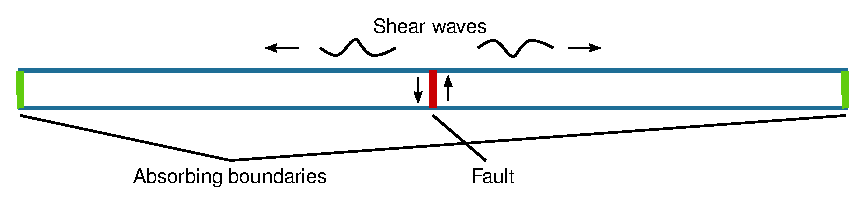
\includegraphics{tutorials/shearwave/figs/bar}
\par\end{centering}

\caption{Domain for shear wave propagation in a 8.0 km bar with 400 m cross-section.
We generate a shear wave via slip on a fault located in the middle
of the bar while limiting deformation to the transverse direction.\label{fig:shearwave:domain}}
\end{figure}


For the bar discretized with quad4 cells we also consider the fault
subjected to frictional sliding controlled by static friction, linear
slip-weakening friction, and rate- and state-friction. We use initial
tractions applied to the fault to drive the dislocation and generate
the shear wave. Because the fault tractions are constant in time,
they continue to drive the motion even after the shear wave reaches
the absorbing boundary, leading to a steady state solution with uniform
shear deformation in the bar and a constant slip rate on the fault. 

[pylithapp]

# ----------------------------------------------------------------------
# Monitoring and parameter viewing.
# ----------------------------------------------------------------------
dump_parameters.filename = output/tri3-parameters.json

# ----------------------------------------------------------------------
# mesh_generator
# ----------------------------------------------------------------------
[pylithapp.mesh_generator]
reader.filename = tri3.exo

# ----------------------------------------------------------------------
# solution
# ----------------------------------------------------------------------
[pylithapp.problem.solution_observers.domain]
writer.filename = output/tri3-domain.h5

# ----------------------------------------------------------------------
# materials
# ----------------------------------------------------------------------
# Specify the material information for the problem.
[pylithapp.timedependent.materials.maxwell]
observers.observer.writer.filename = output/tri3-maxwell.h5

# ----------------------------------------------------------------------
# boundary conditions
# ----------------------------------------------------------------------
[pylithapp.problem.bc.y_neg]
observers.observer.writer.filename = output/tri3-y_neg.h5

[pylithapp.problem.bc.y_pos]
observers.observer.writer.filename = output/tri3-y_pos.h5

[pylithapp.problem.bc.x_neg]
observers.observer.writer.filename = output/tri3-x_neg.h5

[pylithapp.problem.bc.x_pos]
observers.observer.writer.filename = output/tri3-x_pos.h5

# End of file

\section{\label{sec:tutorial:shearwave:tet4}3D Bar Discretized with Tetrahedra}

PyLith features discussed in this tutorial:
\begin{itemize}
\item Dynamic solution
\item LaGriT mesh format
\item Absorbing dampers boundary conditions
\item Kinematic fault interface conditions
\item Elastic isotropic linearly elastic material
\item VTK output
\item Linear tetrahedral cells
\item SimpleDB spatial database
\item ZeroDispDB spatial database
\end{itemize}
All of the files necessary to run the examples are contained in the
directory \texttt{examples/bar\_shearwave/tet4.}


\subsection{Mesh Generation}

The mesh is a simple rectangular prism 8 km by 400 m by 400m (Figure
\ref{fig:shearwave:tet4:mesh}). This mesh could be generated via
a simple script, but it is even easier to generate this mesh using
LaGriT. We provide documented LaGriT files in \texttt{examples/bar\_shearwave/tet4.}
We first create the geometry and regions, mesh the domain using tetrahedral
cells, and then create point sets associated with boundary conditions.

\noindent \begin{center}
\begin{figure}
\begin{centering}
\includegraphics[scale=0.5]{tutorials/shearwave/figs/tet4mesh}
\par\end{centering}

\caption{Mesh composed of tetrahedral cells generated by LaGriT used for the
example problem.\label{fig:shearwave:tet4:mesh}}
\end{figure}

\par\end{center}


\subsection{Simulation Parameters}

The simulation parameters match those in the tri3 example with the
exception of using the LaGriT mesh reader and switching from a two-dimensional
problem to a three-dimensional problem. In addition to fixing the
longitudinal degree of freedom, we also fix the out-of-plane transverse
degree of freedom. Because the fault separates two material regions
in LaGriT, we use two materials in PyLith. All of the parameters are
set in the \texttt{pylithapp.cfg} file. To run the problem, simply
run PyLith without any command line arguments:
\begin{lyxcode}
pylith
\end{lyxcode}
The VTK files will be written to the \texttt{output} directory. The
output includes the displacement and velocity fields over the entire
domain at every 3rd time step (0.10 s), the slip and change in traction
vectors on the fault surface in along-strike and normal directions
at every 3rd time step (0.10 s), and the strain and stress tensors
for each cell at every 30th time step (1.0 s). If the problem ran
correctly, you should be able to generate a figure such as Figure
\ref{fig:shearwave:tet4:deform}, which was generated using ParaView.

\noindent \begin{center}
\begin{figure}
\begin{centering}
\includegraphics[scale=0.5]{tutorials/shearwave/figs/tet4deform30}
\par\end{centering}

\caption{Displacement field in the bar at 3.0 s. Deformation has been exaggerated
by a factor of 800.\label{fig:shearwave:tet4:deform}}
\end{figure}

\par\end{center}

\section{\label{sec:tutorial:shearwave:hex8}3D Bar Discretized with Hexahedra}

PyLith features discussed in this tutorial:
\begin{itemize}
\item Dynamic solution
\item CUBIT mesh format
\item Absorbing dampers boundary conditions
\item Kinematic fault interface conditions
\item Elastic isotropic linearly elastic material
\item VTK output
\item Linear hexahedral cells
\item SimpleDB spatial database
\item ZeroDispDB spatial database
\end{itemize}
All of the files necessary to run the examples are contained in the
directory \texttt{examples/bar\_shearwave/hex8.}


\subsection{Mesh Generation}

The mesh is a simple rectangular prism 8 km by 400 m by 400 m (Figure
\ref{fig:shearwave:hex8:mesh}). This mesh could be generated via
a simple script, but it is even easier to generate this mesh using
CUBIT. We provide documented CUBIT journal files in \texttt{examples/bar\_shearwave/hex8.}
We first create the geometry, mesh the domain using hexahedral cells,
and then create blocks and nodesets associated with the materials
and boundary conditions.

\noindent \begin{center}
\begin{figure}
\begin{centering}
\includegraphics[scale=0.5]{tutorials/shearwave/figs/hex8mesh}
\par\end{centering}

\caption{Mesh composed of hexahedral cells generated by CUBIT used for the
example problem.\label{fig:shearwave:hex8:mesh}}
\end{figure}

\par\end{center}


\subsection{Simulation Parameters}

The simulation parameters match those in the tri3 and tet4 examples.
As in the tet4 example, we fix both the longitudinal degree of freedom
and the out-of-plane transverse degree of freedom. Using eight-point
quadrature permits use of a time step of 1/20 s, which is slightly
larger than the time step of 1/30 s used in the tri3 and tet4 simulations.
All of the parameters are set in the \texttt{pylithapp.cfg} file.
To run the problem, simply run PyLith without any command line arguments:
\begin{lyxcode}
pylith
\end{lyxcode}
The VTK files will be written to the \texttt{output} directory. The
output includes the displacement and velocity fields over the entire
domain at every other time step (0.10 s), the slip and change in traction
vectors on the fault surface in along-strike and normal directions
at every other time step (0.10 s), and the strain and stress tensors
for each cell at every 20th time step (1.0 s). If the problem ran
correctly, you should be able to generate a figure such as Figure
\ref{fig:shearwave:hex8:deform}, which was generated using ParaView.

\noindent \begin{center}
\begin{figure}
\begin{centering}
\includegraphics[scale=0.5]{tutorials/shearwave/figs/hex8deform30}
\par\end{centering}

\caption{Displacement field in the bar at 3.0 s. Deformation has been exaggerated
by a factor of 800.\label{fig:shearwave:hex8:deform}}
\end{figure}

\par\end{center}

\section{\label{sec:tutorial:shearwave:quad4}3D Bar Discretized with Quadrilaterals}

PyLith features discussed in this tutorial:
\begin{itemize}
\item Dynamic solution
\item CUBIT mesh format
\item Absorbing dampers boundary conditions
\item Kinematic fault interface conditions
\item Dynamic fault interface conditions
\item Plane strain linearly elastic material
\item VTK output
\item Linear quadrilateral cells
\item SimpleDB spatial database
\item ZeroDispDB spatial database
\item UniformDB spatial database
\end{itemize}
All of the files necessary to run the examples are contained in the
directory \texttt{examples/bar\_shearwave/quad4.}


\subsection{Mesh Generation}

The mesh is a simple rectangular prism 8 km by 400 m by 400 m (Figure
\ref{fig:shearwave:quad4:mesh}). We provide documented CUBIT journal
files in \texttt{examples/bar\_shearwave/quad4.} We first create the
geometry, mesh the domain using quadrilateral cells, and then create
blocks and nodesets associated with the materials and boundary conditions.

\noindent \begin{center}
\begin{figure}
\begin{centering}
\includegraphics[scale=0.5]{tutorials/shearwave/figs/quad4mesh}
\par\end{centering}

\caption{Mesh composed of hexahedral cells generated by CUBIT used for the
example problem.\label{fig:shearwave:quad4:mesh}}
\end{figure}

\par\end{center}


\subsection{Kinematic Fault (Prescribed Slip)}

The simulation parameters match those in the tri3, tet4, and hex8
examples. Using four-point quadrature permits use of a time step of
1/20 s, which is slightly larger than the time step of 1/30 s used
in the tri3 and tet4 simulations. In contrast to the tri3, tet4, and
hex8 shear wave examples which only contained a single simulation
in a directory, in this example we consider several different simulations.
Consequently, we separate the parameters into multiple \texttt{.cfg}
files. The common parameters are placed in \texttt{pylithapp.cfg}
with the parameters specific to the kinematic fault (prescribed rupture)
example in \texttt{prescribedrup.cfg}. To run the problem, simply
run PyLith via:
\begin{lyxcode}
pylith~prescribedrup.cfg
\end{lyxcode}
The VTK files will be written to the \texttt{output} directory with
the prefix \texttt{prescribedrup}. The output includes the displacement
field over the entire domain at every other time step (0.10 s), the
slip and traction vectors on the fault surface in along-strike and
normal directions at every other time step (0.10 s), and the strain
and stress tensors for each cell at every 20th time step (1.0 s).
If the problem ran correctly, you should be able to generate a figure
such as Figure \ref{fig:shearwave:quad4:kinematic}, which was generated
using ParaView.

\noindent \begin{center}
\begin{figure}
\begin{centering}
\includegraphics[scale=0.5]{tutorials/shearwave/figs/quad4kinematic30}
\par\end{centering}

\caption{Displacement field in the bar at 3.0 s. Deformation has been exaggerated
by a factor of 800.\label{fig:shearwave:quad4:kinematic}}
\end{figure}

\par\end{center}


\subsection{Dynamic Fault (Spontaneous Rupture)}

In this set of examples we replace the kinematic fault interface with
the dynamic fault interface, resulting in fault slip controlled by
a fault-constitutive model. See Section \ref{sec:fault:constitutive:models}
for detailed information about the fault constitutive models available
in PyLith. Because this is a dynamic simulation we want the generated
shear wave to continue to be absorbed at the ends of the bar, so we
drive the fault by imposing initial tractions directly on the fault
surface rather than through deformation within the bar. We impose
initial tractions (75 MPa of right-lateral shear and 120 MPa of compression)
plus a temporal variation (smoothly increasing from 0 to 25 MPa of
right-lateral shear) similar to what would be used in a 2-D or 3-D
version. While the magnitude of these stresses is reasonable for tectonic
problems, they give rise to very large slip rates in this 1-D bar.
The temporal variation, as specified via the \texttt{traction\_change.timedb}
file, has the functional form:
\begin{equation}
f(t)=\begin{cases}
\exp\left(\frac{\left(t-t_{n}\right)^{2}}{t\left(t-2t_{n}\right)}\right), & 0<t\le t_{n}\\
1, & t>t_{n}
\end{cases}
\end{equation}
where $t_{n}$ = 1.0 s. We request that the fault output include the
initial traction value and the slip, slip rate, and traction fields:
\begin{lyxcode}
{[}pylithapp.timedependent.interfaces.fault.output{]}

vertex\_info\_fields={[}traction\_initial\_value{]}

vertex\_data\_fields~=~{[}slip,slip\_rate,traction{]}
\end{lyxcode}
The steady-state solution for this problem is constant velocity and
slip rate with uniform strain within the bar. A Python script, \texttt{analytical\_soln.py},
is included for computing values related to the steady-state solution.


\subsubsection{Dynamic Fault with Static Friction}

The parameters specific to this example involve the static friction
fault constitutive model. We set the fault constitutive model via
\begin{lyxcode}
{[}pylithapp.timedependent.interfaces.fault{]}

friction~=~pylith.friction.StaticFriction
\end{lyxcode}
and use a UniformDB to set the static friction parameters. We use
a coefficient of friction of 0.6 and no cohesion (0 MPa). The parameters
specific to this example are in \texttt{spontaneousrup\_staticfriction.cfg},
so we run the problem via:
\begin{lyxcode}
pylith~spontaneousrup.cfg~spontaneousrup\_staticfriction.cfg
\end{lyxcode}
The VTK files will be written to the \texttt{output} directory with
the prefix \texttt{staticfriction}. The output includes the displacement
and velocity fields over the entire domain at every other time step
(0.10 s), the slip, slip rate, and traction vectors on the fault surface
in along-strike and normal directions at every other time step (0.10
s), and the strain and stress tensors for each cell at every 20th
time step (1.0 s). If the problem ran correctly, you should be able
to generate a figure such as Figure \ref{fig:shearwave:quad4:staticfriction},
which was generated using ParaView. The steady-state solution is a
constant slip rate of 22.4 m/s, a shear traction of 72.0 MPa on the
fault surface, a uniform shear strain of 5.6e-3 in the bar with uniform,
and constant velocities in the y-direction of +11.2 m/s and -11.2
m/s on the -x and +x sides of the fault, respectively.

\noindent \begin{center}
\begin{figure}
\begin{centering}
\includegraphics[scale=0.5]{tutorials/shearwave/figs/quad4staticfriction30}
\par\end{centering}

\caption{Velocity field in the bar at 3.0 s for the static friction fault constitutive
model. Deformation has been exaggerated by a factor of 20.\label{fig:shearwave:quad4:staticfriction}}
\end{figure}

\par\end{center}


\subsubsection{Dynamic Fault with Slip-Weakening Friction}

The parameters specific to this example are related to the use of
the slip-weakening friction fault constitutive model (see Section
\ref{sec:fault:constitutive:models}). We set the fault constitutive
model via
\begin{lyxcode}
{[}pylithapp.timedependent.interfaces.fault{]}

friction~=~pylith.friction.SlipWeakening
\end{lyxcode}
and use a UniformDB to set the slip-weakening friction parameters.
We use a static coefficient of friction of 0.6, a dynamic coefficient
of friction of 0.5, a slip-weakening parameter of 0.2 m, and no cohesion
(0 MPa). The fault constitutive model is associated with the fault,
so we can append the fault constitutive model parameters to the vertex
information fields:
\begin{lyxcode}
{[}pylithapp.timedependent.interfaces.fault.output{]}

vertex\_info\_fields~=~{[}strike\_dir,normal\_dir,initial\_traction,static\_coefficient,~\\
dynamic\_coefficient,slip\_weakening\_parameter,cohesion{]}
\end{lyxcode}
The parameters specific to this example are in \texttt{spontaneousrup\_slipweakening.cfg},
so we run the problem via:
\begin{lyxcode}
pylith~spontaneousrup.cfg~spontaneousrup\_slipweakening.cfg
\end{lyxcode}
The VTK files will be written to the \texttt{output} directory with
the prefix \texttt{slipweakening}. If the problem ran correctly, you
should be able to generate a figure such as Figure \ref{fig:shearwave:quad4:slipweakening},
which was generated using ParaView. The steady-state solution is a
constant slip rate of 32.0 m/s and shear traction of 60.0 MPa on the
fault surface, a uniform shear strain of 8.0e-3 in the bar with uniform,
constant velocities in the y-direction of +16.0 m/s and -46.0 m/s
on the -x and +x sides of the fault, respectively.

\noindent \begin{center}
\begin{figure}
\begin{centering}
\includegraphics[scale=0.5]{tutorials/shearwave/figs/quad4slipweakening30}
\par\end{centering}

\caption{Velocity field in the bar at 3.0 s for the slip-weakening friction
fault constitutive model. Deformation has been exaggerated by a factor
of 20.\label{fig:shearwave:quad4:slipweakening}}
\end{figure}

\par\end{center}


\subsubsection{Dynamic Fault with Rate-State Friction}

The parameters specific to this example are related to the use of
the rate- and state-friction fault constitutive model (see Section
\ref{sec:fault:constitutive:models}). The evolution of the state
variable uses the ageing law. We set the fault constitutive model
and add the state variable to the output via
\begin{lyxcode}
{[}pylithapp.timedependent.interfaces.fault{]}

friction~=~pylith.friction.RateStateAgeing~\\


{[}pylithapp.timedependent.interfaces.fault.output{]}~\\
vertex\_data\_fields~=~{[}slip,~slip\_rate,~traction,~state\_variable{]}~
\end{lyxcode}
and use a UniformDB to set the rate-state friction parameters. We
use a reference coefficient of friction of 0.6, reference slip rate
of 1.0e-6 m/s, characteristic slip distance of 0.02 m, coefficients
a and b of 0.008 and 0.012, and no cohesion (0 MPa). We set the initial
value of the state variable so that the fault is in equilibrium for
the initial tractions. The parameters specific to this example are
in \texttt{spontaneousrup\_ratestateageing.cfg}, so we run the problem
via:
\begin{lyxcode}
pylith~spontaneousrup.cfg~spontaneousrup\_ratestateageing.cfg
\end{lyxcode}
The VTK files will be written to the \texttt{output} directory with
the prefix \texttt{ratestateageing}. If the problem ran correctly,
you should be able to generate a figure such as Figure \ref{fig:shearwave:quad4:ratestateageing},
which was generated using ParaView. The steady-state solution is a
constant slip rate of 30.0 m/s and shear traction of 63.7 MPa on the
fault surface, a uniform shear strain of 7.25e-3 in the bar with uniform,
constant velocities in the y-direction of +15.0 m/s and -15.0 m/s
on the -x and +x sides of the fault, respectively.

\noindent \begin{center}
\begin{figure}
\begin{centering}
\includegraphics[scale=0.5]{tutorials/shearwave/figs/quad4ratestateageing30}
\par\end{centering}

\caption{Velocity field in the bar at 3.0 s for the rate- and state-friction
fault constitutive model. Deformation has been exaggerated by a factor
of 20.\label{fig:shearwave:quad4:ratestateageing}}
\end{figure}

\par\end{center}




\section{Additional Examples}


\subsection{CUBIT Meshing Examples}

The directory \filename{examples/meshing} contains several examples
of using CUBIT to construct finite-element meshes for complex geometry.
This includes features such as constructing nonplanar fault geometry
from contours, constructing topography from a DEM, and merging sheet
bodies (surfaces). A separate examples discusses defining the discretization
size using a vertex field in an Exodus-II file. See the \filename{README}
files in the subdirectories for more detailed descriptions of these
examples.


\subsection{Troubleshooting Examples}
\label{sub:troubleshooting:examples}

The directory \filename{examples/troubleshooting} contains a few examples to
practice troubleshooting a variety of user errors in parameters files and
problem setup. The files with the errors corrected are in
\filename{examples/troubleshooting/correct}.  Step-by-step corrections are
discussed in the troubleshooting PyLith simulations sessions of the
2014, 2015, 2017, and 2019 PyLith tutorials
(\url{wiki.geodynamics.org/software:pylith:start}).


\subsection{Code Verification Benchmarks}

The CIG GitHub software repository \url{https://github.com/geodynamics/pylith_benchmarks}
contains input files for a number of community benchmarks. The benchmarks
do not include the mesh files because they are so large; instead they
include the CUBIT journal files that can be used to generate the meshes.
Most, but not all, of the input files in the repository are updated
for PyLith v2.0.0, so you will need to modify them if you use another
version of PyLith.

% End of file


\chapter{\label{cha:Benchmarks}Benchmarks}


\section{Overview}

The Crustal Deformation Modeling and Earthquake Source Physics Focus
Groups within the Southern California Earthquake Center and the Short-Term
Tectonics Working Group within CIG have developed a suite of benchmarks
to test the accuracy and performance of 3D numerical codes for quasi-static
crustal deformation and earthquake rupture dynamics. The benchmark
definitions for the quasi-static crustal deformation benchmarks are
posted on the CIG website at Short-Term Tectonics Benchmarks \url{geodynamics.org/cig/workinggroups/short/workarea/benchmarks/}
and the definitions for the earthquake rupture benchmarks are posted
on the SCEC website \url{scecdata.usc.edu/cvws/cgi-bin/cvws.cgi}.
This suite of benchmarks permits evaluating the relative performance
of different types of basis functions, quadrature schemes, and discretizations
for geophysical applications. The files needed to run the 3D benchmarks
are in the CIG GitHub Repository \url{https://github.com/geodynamics/pylith_benchmarks}.
In addition to evaluating the efficiency and accuracy of numerical
codes, the benchmarks also make good test problems, where users can
perform simulations based on actual geophysical problems. The benchmarks
are performed at various resolutions and using different element types.
By comparing the runtime and accuracy for different resolutions and
element types, users can evaluate which combination will be best for
their problems of interest.

\input{benchmarks/strikeslip/strikeslip.tex}
\section{\label{sec:benchmarks:savageprescott}Savage and Prescott Benchmark}

This benchmark problem computes the viscoelastic (Maxwell) relaxation
of stresses from repeated infinite, strike-slip earthquakes in 3D
without gravity. The files needed to run the benchmark may be found
at \url{https://github.com/geodynamics/pylith_benchmarks/tree/master/quasistatic/sceccrustdeform/savageprescott}.
An analytical solution to this problem is described by Savage and
Prescott \cite{Savage:Prescott:1978}, which provides a simple way
to check our numerical solution. A python utility code is provided
in the utils directory to compute the analytical solution. Although
this problem is actually 2.5D (infinite along-strike), we solve it
using a 3D finite element model.


\subsection{Problem Description}

Figure \ref{fig:benchmark:savageprescott:geometry} shows the geometry
of the problem, as described by \cite{Savage:Prescott:1978}. The
analytical solution describes the surface deformation due to repeated
earthquakes on an infinite strike-slip fault embedded in an elastic
layer overlying a Maxwell viscoelastic half-space. The upper portion
of the fault (red in the figure) is locked between earthquakes, while
the lower portion (blue in the figure) creeps at plate velocity. At
regular recurrence intervals, the upper portion of the fault abruptly
slips by an amount equal to the plate velocity multiplied by the recurrence
interval, thus 'catching up' with the lower part of the fault.

There are some differences between the analytical solution and our
numerical representation. First, the analytical solution represents
the earthquake cycle as the superposition of uniform fault creep and
an elementary earthquake cycle. Uniform fault creep is simply the
uniform movement of the two plates past each other at plate velocity.
For the elementary earthquake cycle, no slip occurs below the locked
portion of the fault (blue portion in the figure). On the locked (red)
portion of the fault, backslip equal to plate velocity occurs until
the earthquake recurrence interval, at which point abrupt forward
slip occurs. In the finite element solution, we perform the simulation
as described in the figure. Velocity boundary conditions are applied
at the extreme edges of the model to simulate block motion, steady
creep is applied along the blue portion of the fault, and regular
earthquakes are applied along the upper portion of the fault. It takes
several earthquake cycles for the velocity boundary conditions to
approximate the steady flow due to steady block motion, so we would
not expect the analytical and numerical solutions to match until several
earthquakes have occurred. Another difference lies in the dimensions
of the domain. The analytical solution assumes an infinite strike-slip
fault in an elastic layer overlying a Maxwell viscoelastic half-space.
In our finite element model we are restricted to finite dimensions.
We therefore extend the outer boundaries far enough from the region
of interest to approximate boundaries at infinity.

Due to the difficulties in representing solutions in an infinite domain,
there are several meshes that have been tested for this problem. The
simplest meshes have uniform resolution (all cells have equal dimensions);
however, such meshes typically do not provide accurate solutions since
the resolution is too coarse in the region of interest. For that reason,
we also tested meshes where the mesh resolution decreases away from
the center. In the problem description that follows, we will focus
on the hexahedral mesh with finer discretization near the fault \linebreak{}
(\texttt{meshes/hex8\_6.7km.exo.gz}), which provides a good match
with the analytical solution. It will first be necessary to gunzip
this mesh so that it may be used by PyLith.
\begin{description}
\item [{Domain}] The domain for this mesh spans the region
\begin{gather*}
-1000\leq x\leq1000\ km,\\
-500\leq y\leq500\ km,\\
-400\ km\leq z\leq0.
\end{gather*}
The top (elastic) layer occupies the region $-40\ km\ \leq z\leq0$
and the bottom (viscoelastic) layer occupies the region $-400\ km\ \leq z\leq-40\ km$.
\item [{Material~properties}] The material is a Poisson solid with a shear
modulus ($\mu$) of 30 GPa. The domain is modeled using an elastic
isotropic material for the top layer and a Maxwell viscoelastic material
for the bottom layer. The bottom layer has a viscosity ($\eta$) of
2.36682e+19 Pa-s, yielding a relaxation time ($2\eta/\mu$) of 50
years.
\item [{Fault}] The fault is a vertical, left-lateral strike-slip fault.
The strike is parallel to the y-direction at the center of the model:
\begin{gather*}
x=0\ km,\\
-500\leq y\leq500\ km,\\
-40\ km\leq z\leq0.
\end{gather*}
The locked portion of the fault (red section in Figure \ref{fig:benchmark:savageprescott:geometry})
extends from $-20\: km\leq z\leq0$, while the creeping section (blue)
extends from $-40\: km\leq z\leq0$. Along the line where the two
sections coincide ($z=-20\: km$), half of the coseismic displacement
and half of the steady creep is applied (see \texttt{finalslip.spatialdb}
and \texttt{creeprate.spatialdb}).
\item [{Boundary~conditions}] On the bottom boundary, vertical displacements
are set to zero, while on the y-boundaries the x-displacements are
set to zero. On the x-boundaries, the x-displacements are set to zero,
while constant velocities of +/- 1 cm/yr are applied in the y-direction,
giving a relative plate motion of 2 cm/year.
\item [{Discretization}] For the nonuniform hexahedral mesh, the resolution
at the outer boundaries is 20 km. An inner region is then put through
one level of refinement, so that near the center of the mesh the resolution
is 6.7 km. All meshes were generated with CUBIT.
\item [{Basis~functions}] We use trilinear hexahedral cells.
\item [{Solution}] We compute the surface displacements and compare these
to the analytical solution in Figure \ref{fig:benchmark:savageprescott:solution}.
\end{description}
\noindent \begin{center}
\begin{figure}[H]
\begin{centering}
\includegraphics[scale=0.33]{benchmarks/savageprescott/figs/model_descript}
\par\end{centering}

\caption{Problem description for the Savage and Prescott strike-slip benchmark
problem.\label{fig:benchmark:savageprescott:geometry}}
\end{figure}

\par\end{center}


\subsection{Running the Benchmark}

After checking out the benchmark files from the CIG SVN repository,
change to the \texttt{meshes} directory. Decompress the gzipped files
in the \texttt{mesh} directory,
\begin{lyxcode}
gunzip~{*}.gz
\end{lyxcode}
Alternatively, simply gunzip the mesh you want to use. There are a
number of \texttt{.cfg} files corresponding to the different meshes,
as well as a \texttt{pylithapp.cfg} file defining parameters common
to all problems. Each problem uses four \texttt{.cfg} files: \texttt{pylithapp.cfg},
\texttt{fieldsplit.cfg} (algrebraic multigrid preconditioner), a cell-specific
file (e.g., \texttt{hex8.cfg}), and a resolution specific file (e.g.,
hex8\_6.7km.cfg). You can then run the problem by typing
\begin{lyxcode}
pylith~hex8.cfg~hex8\_6.7km.cfg~fieldsplit.cfg
\end{lyxcode}
This will run the problem for 10 earthquake cycles of 200 years each,
using a time-step size of 10 years, for a total simulation time of
2000 years. Ground surface output occurs every 10 years, while all
other outputs occur every 50 years.

Once the problem has run, results will be placed in the \texttt{output}
directory. These results may be viewed directly with a package such
as ParaView; however, to compare results to the analytical solution,
some postprocessing is required. First, generate the analytical results
by running the \texttt{calc\_analytic.py} script. This will produce
files with displacements and velocities (\texttt{analytic\_disp.txt}
and \texttt{analytic\_vel.txt}) in the \texttt{output} directory that
are easy to use with a plotting package, such as matplotlib or Matlab.


\subsection{Benchmark Results}

Figure \ref{fig:benchmark:savageprescott:solution} shows the computed
surface displacements for the 10th earthquake cycle compared with
the analytical solution. The profile results were obtained as described
above, and then all results (analytical and numerical) were referenced
to the displacements immediately following the last earthquake. We
find very good agreement between the analytical and numerical solutions,
even for meshes with uniform refinement. We have not yet explored
quantitative fits as a function of mesh resolution. For this benchmark,
it is also important to consider the distance of the boundary from
the region of interest. Also note that the agreement between analytical
and numerical solutions is poor for early earthquake cycles, due to
the differences in simulating the problem, as noted above.

\begin{figure}
\begin{centering}
\includegraphics[scale=0.66]{benchmarks/savageprescott/figs/soln_profiles}
\par\end{centering}

\caption{Displacement profiles perpendicular to the fault for a PyLith simulation
with hex8 cells and the analytical solution for earthquake cycle 10.
\label{fig:benchmark:savageprescott:solution}}
\end{figure}




\section{SCEC Dynamic Rupture Benchmarks}

The SCEC website \url{scecdata.usc.edu/cvws/cgi-bin/cvws.cgi} includes
a graphical user interface for examining the benchmark results. Benchmark
results for PyLith are available for TPV205-2D (horizontal slice through
a vertical strike-slip fault), TPV205 (vertical strike-slip fault
with high and low stress asperities), TPV210-2D (vertical slice through
a 60-degree dipping normal fault), TPV210 (60-degree dipping normal
fault), TPV11, TPV12, TPV13, TPV14-2D and TPV15-2D (horizontal slice
through a verticel strike-slip fault with a branch), TPV14, TPV15,
TPV 24, TPV25 (vertical strike-slip fault with a branch), TPV 16 and
17 (vertical strike-slip fault with spatially heterogeneous initial
tractions), TPV 22 and 23 (vertical strike-slip fault with a stepover),
TPV102 (vertical strike-slip fault with rate-state friction).

The benchmark results indicate that triangular and tetrahedral cells
generate less numerical noise than quadrilateral or hexahedral cells.
The input files in the repository are updated for PyLith v2.0.0, so
you will need to modify them if you use another version of PyLith.


\appendix

\chapter{\label{cha:Glossary}Glossary}


\section{Pyre}
\begin{description}
\item [{component}] Basic building block of a Pyre application. A component
may be built-up from smaller building blocks, where simple data types
are called properties and data structures and objects are called facilities.
In general a component is a specific implementation of the functionality
of a facility. For example, SimpleDB is a specific implementation
of the spatial database facility. A component is generally composed
of a Python object and a C++ object, although either one may be missing.
We nearly always use the naming convention such that for an object
called Foo the Python object is in file Foo.py, the C++ class definition
is in Foo.hh, inline C++ functions are in foo.icc, the C++ class implementation
is in Foo.cc, and the SWIG interface file that glues the C++ and Python
code together is in Foo.i.
\item [{facility}] Complex data type (object or data structure) building
block of a component. See component.
\item [{property}] Simple data type (string, integer, real number, or boolean
value) parameter for a component.
\end{description}

\section{DMPlex}
\begin{description}
\item [{DMPlex}] The plex construction is a representation of the topology
of the finite element mesh based upon a covering relation. For example,
segments are covered by their endpoints, faces by their bounding edges,
etc. Geometry is absent from the plex, and is represented instead
by a  field with the coordinates of the vertices. Meshes can also
be understood as directed acyclic graphs, where we call the constituents
points and arrows.
\item [{mesh}] A finite element mesh, used to partition space and provide
support for the basis functions.
\item [{cell}] The highest dimensional elements of a mesh, or mesh entities
of codimension zero.
\item [{vertex}] The zero dimensional mesh elements.
\item [{face}] Mesh elements that separate cells, or mesh entities of codimension
one.
\item [{field}] A parallel section which can be completed, or made consistent,
across process boundaries. These are used to represent continuum fields.
\item [{section}] These objects associate values in vectors to points (vertices,
 edges, faces, and cells) in a mesh. The section describes the offset
 into the vector along with the number of values associated with each
point.
\item [{dimension}] The topological dimension of the mesh, meaning the
cell dimension. It can also mean the dimension of the space in which
the mesh is embedded, but this is properly the embedding dimension.
\item [{fiber\ dimension}] Dimension of the space associated with the
field. For example, the scalar field has a fiber dimension of 1 and
a vector field has a fiber displacement equal to the dimension of
the mesh.
\item [{cohesive\ cell}] A zero volume cell inserted between any two cells
which shared a fault face. They are prisms with a fault face as the
base.
\item [{cone}] The set of entities which cover any entity in a mesh. For
example, the cone of a triangle is its three edges.
\item [{support}] The set of mesh entities which are covered by any entity
in a mesh. For example, the support of a triangle is the two tetrahedra
it separates.
\end{description}



\chapter{\label{cha:components}PyLith and Spatialdata Components}

The name of the component is followed by the full path name and description.
The full path name is used when setting a component to a facility
in a \texttt{.cfg} file or with command line arguments.


\section{Application components}
\begin{description}
\item [{\texttt{PyLithApp}}] \texttt{pylith.apps.PyLithApp}\\
PyLith application.
\end{description}

\subsection{Problem Components}
\begin{description}
\item [{\texttt{TimeDependent}}] \texttt{pylith.problems.TimeDependent}\\
Time-dependent problem.
\item [{\texttt{GreensFns}}] \texttt{pylith.problems.GreensFns}\\
Static Green's function problem with slip impulses.
\item [{\texttt{Implicit}}] \texttt{pylith.problems.Implicit}\\
Implicit time stepping for static and quasi-static simulations with
infinitesimal strains.
\item [{\texttt{ImplicitLgDeform}}] \texttt{pylith.problems.ImplicitLgDeform}\\
Implicit time stepping for static and quasi-static simulations including
the effects of rigid body motion and small strains.
\item [{\texttt{Explicit}}] \texttt{pylith.problems.Explicit}\\
Explicit time stepping for dynamic simulations with a lumped system
Jacobian matrix.
\item [{\texttt{ExplicitLgDeform}}] \texttt{pylith.problems.ExplicitLgDeform}\\
Explicit time stepping for dynamic simulations including the effects
of rigid body motion and small strains with a lumped system Jacobian
matrix.
\item [{\texttt{ExplicitTri3}}] \texttt{pylith.problems.ExplicitTri3}\\
Optimized elasticity formulation for linear triangular cells and one
quadrature point for explicit time stepping in dynamic simulations.
\item [{\texttt{ExplicitTet4}}] \texttt{pylith.problems.ExplicitTet4}\\
Optimized elasticity formulation for linear tetrahedral cells and
one quadrature point for explicit time stepping in dynamic simulations.
\item [{\texttt{SolverLinear}}] \texttt{pylith.problems.SolverLinear}\\
Linear PETSc solver (KSP).
\item [{\texttt{SolverNonlinear}}] \texttt{pylith.problems.SolverNonlinear}\\
Nonlinear PETSc solver (SNES).
\item [{\texttt{SolverLumped}}] \texttt{pylith.problems.SolverLumped}\\
Built-in simple, optimized solver for solving systems with a lumped
Jacobian.
\item [{\texttt{TimeStepUniform}}] \texttt{pylith.problems.TimeStepUniform}\\
Uniform time stepping.
\item [{\texttt{TimeStepAdapt}}] \texttt{pylith.problems.TimeStepAdapt}\\
Adaptive time stepping (time step selected based on estimated stable
time step).
\item [{\texttt{TimeStepUser}}] \texttt{pylith.problems.TimeStepUser}\\
User defined time stepping (variable time step set by user).
\end{description}

\subsection{Utility Components}
\begin{description}
\item [{\texttt{NullComponent}}] \texttt{pylith.utils.NullComponent}\\
Null component used to set a facility to an empty value.
\item [{\texttt{EventLogger}}] \texttt{pylith.utils.EventLogger}\\
PETSc event logger.
\item [{\texttt{VTKDataReader}}] \texttt{pylith.utils.VTKDataReader}\\
Data reader for VTK files, requires TVTK Enthought package available
from \texttt{}~\\
\texttt{https://github.com/enthought/mayavi.}
\end{description}

\subsection{Topology Components}
\begin{description}
\item [{\texttt{Distributor}}] \texttt{pylith.topology.Distributor}\\
Distributor of mesh among processors in parallel simulations.
\item [{\texttt{JacobianViewer}}] \texttt{pylith.topology.JacobianViewer}\\
Viewer for writing Jacobian sparse matrix to file.
\item [{\texttt{MeshGenerator}}] \texttt{pylith.topology.MeshGenerator}\\
Mesh generator/importer.
\item [{\texttt{MeshImporter}}] \texttt{pylith.topology.MeshImporter}\\
Mesh importer/reader.
\item [{\texttt{MeshRefiner}}] \texttt{pylith.topology.MeshRefiner}\\
Default (null) mesh refinement object that does not refine the mesh.
\item [{\texttt{RefineUniform}}] \texttt{pylith.topology.RefineUniform}\\
Uniform global mesh refinement.
\item [{\texttt{ReverseCuthillMcKee}}] \texttt{pylith.topology.ReverseCuthillMcKee}\\
Object used to manage reordering cells and vertices using the reverse
Cuthill-McKee algorithm.
\end{description}

\subsection{Material Components}
\begin{description}
\item [{\texttt{ElasticStrain1D}}] \texttt{pylith.materials.ElasticStrain1D}\\
Linearly elastic 1D bulk constitutive model with 1D strain ($\epsilon_{yy}=\epsilon_{zz}=0$).
\item [{\texttt{ElasticStress1D}}] \texttt{pylith.materials.ElasticStress1D}\\
Linearly elastic 1D bulk constitutive model with 1D stress ($\sigma_{yy}=\sigma_{zz}=0$).
\item [{\texttt{ElasticPlaneStrain}}] \texttt{pylith.materials.ElasticPlaneStrain}\\
Linearly elastic 2D bulk constitutive model with plane strain ($\epsilon_{zz}=0$).
\item [{\texttt{ElasticPlaneStress}}] \texttt{pylith.materials.ElasticPlaneStress}\\
Linearly elastic 2D bulk constitutive model with plane stress ($\sigma_{zz}=0$).
\item [{\texttt{ElasticIsotropic3D}}] \texttt{pylith.materials.ElasticIsotropic3D}\\
Linearly elastic 3D bulk constitutive model.
\item [{\texttt{MaxwellIsotropic3D}}] \texttt{pylith.materials.MaxwellIsotropic3D}\\
Linear Maxwell viscoelastic bulk constitutive model.
\item [{\texttt{MaxwellPlaneStrain}}] \texttt{pylith.materials.MaxwellPlaneStrain}\\
Linear Maxwell viscoelastic bulk constitutive model for plane strain
problems.
\item [{\texttt{GenMaxwellIsotropic3D}}] \texttt{pylith.materials.GenMaxwellIsotropic3D}\\
Generalized Maxwell viscoelastic bulk constitutive model.
\item [{\texttt{GenMaxwellPlaneStrain}}] \texttt{pylith.materials.GenMaxwellPlaneStrain}\\
Generalized Maxwell viscoelastic bulk constitutive model for plane
strain problems.
\item [{\texttt{PowerLaw3D}}] \texttt{pylith.materials.PowerLaw3D}\\
Power-law viscoelastic bulk constitutive model.
\item [{\texttt{PowerLawPlaneStrain}}] \texttt{pylith.materials.PowerLawPlaneStrain}\\
Power-law viscoelastic bulk constitutive model for plane strain problems.
\item [{\texttt{DruckerPrage3D}}] \texttt{pylith.materials.DruckerPrager3D}\\
Drucker-Prager elastoplastic bulk constitutive model.
\item [{\texttt{DruckerPragePlaneStrain}}] \texttt{pylith.materials.DruckerPragerPlaneStrain}\\
Drucker-Prager elastoplastic bulk constitutive model for plane strain
problems.
\item [{\texttt{Homogeneous}}] \texttt{pylith.materials.Homogeneous}\\
Container with a single bulk material.
\end{description}

\subsection{Boundary Condition Components}
\begin{description}
\item [{\texttt{AbsorbingDampers}}] \texttt{pylith.bc.AbsorbingDampers}\\
Absorbing boundary condition using simple dashpots.
\item [{\texttt{DirichletBC}}] \texttt{pylith.bc.DirichletBC}\\
Dirichlet (prescribed displacements) boundary condition for a set
of points.
\item [{\texttt{DirichletBoundary}}] \texttt{pylith.bc.DirichletBoundary}\\
Dirichlet (prescribed displacements) boundary condition for a set
of points associated with a boundary surface.
\item [{\texttt{Neumann}}] \texttt{pylith.bc.Neumann}\\
Neumann (traction) boundary conditions applied to a boundary surface.
\item [{\texttt{PointForce}}] \texttt{pylith.bc.PointForce}\\
Point forces applied to a set of vertices.
\item [{\texttt{ZeroDispDB}}] \texttt{pylith.bc.ZeroDispDB}\\
Specialized UniformDB with uniform zero displacements at all degrees
of freedom.
\end{description}

\subsection{Fault Components}
\begin{description}
\item [{\texttt{FaultCohesiveKin}}] \texttt{pylith.faults.FaultCohesiveKin}\\
Fault surface with kinematic (prescribed) slip implemented using cohesive
elements.
\item [{\texttt{FaultCohesiveDyn}}] \texttt{pylith.faults.FaultCohesiveDyn}\\
Fault surface with dynamic (friction) slip implemented using cohesive
elements.
\item [{\texttt{FaultCohesiveImpulses}}] \texttt{pylith.faults.FaultCohesiveImpulses}\\
Fault surface with Green's functions slip impulses implemented using
cohesive elements.
\item [{\texttt{EqKinSrc}}] \texttt{pylith.faults.EqKinSrc}\\
Kinematic (prescribed) slip earthquake rupture.
\item [{\texttt{SingleRupture}}] \texttt{pylith.faults.SingleRupture}\\
Container with one kinematic earthquake rupture.
\item [{\texttt{StepSlipFn}}] \texttt{pylith.faults.StepSlipFn}\\
Step function slip-time function.
\item [{\texttt{ConstRateSlipFn}}] \texttt{pylith.faults.ConstRateSlipFn}\\
Constant slip rate slip-time function.
\item [{\texttt{BruneSlipFn}}] \texttt{pylith.faults.BruneSlipFn}\\
Slip-time function where slip rate is equal to Brune's far-field slip
function.
\item [{\texttt{LiuCosSlipFn}}] \texttt{pylith.faults.LiuCosSlipFn}\\
Slip-time function composed of three sine/cosine functions. Similar
to Brune's far-field time function but with more abrupt termination
of slip.
\item [{\texttt{TimeHistorySlipFn}}] \texttt{pylith.faults.TimeHistorySlipFn}\\
Slip-time function with a user-defined slip time function.
\item [{\texttt{TractPerturbation}}] \texttt{pylith.faults.TractPerturbation}\\
Prescribed traction perturbation applied to fault with constitituve
model in additional to tractions from deformation (generally used
to nucleate a rupture).
\end{description}

\subsection{Friction Components}
\begin{description}
\item [{\texttt{StaticFriction}}] \texttt{pylith.friction.StaticFriction}\\
Static friction fault constitutive model.
\item [{\texttt{SlipWeakening}}] \texttt{pylith.friction.SlipWeakening}\\
Linear slip-weakening friction fault constitutive model.
\item [{\texttt{RateStateAgeing}}] \texttt{pylith.friction.RateStateAgeing}\\
Dieterich-Ruina rate and state friction with ageing law state variable
evolution.
\item [{\texttt{TimeWeakening}}] \texttt{pylith.friction.TimeWeakening}\\
Linear time-weakening friction fault constitutive model.
\end{description}

\subsection{Discretization Components}
\begin{description}
\item [{\texttt{FIATLagrange}}] \texttt{pylith.feassemble.FIATLagrange}\\
Finite-element basis functions and quadrature rules for a Lagrange
reference finite-element cell (point, line, quadrilateral, or hexahedron)
using FIAT. The basis functions are constructed from the tensor produce
of 1D Lagrange reference cells.
\item [{\texttt{FIATSimplex}}] \texttt{pylith.feassemble.FIATSimplex}\\
Finite-element basis functions and quadrature rules for a simplex
finite-element cell (point, line, triangle, or tetrahedron) using
FIAT.
\end{description}

\subsection{Output Components}
\begin{description}
\item [{\texttt{MeshIOAscii}}] \texttt{pylith.meshio.MeshIOAscii}\\
Reader for simple mesh ASCII files.
\item [{\texttt{MeshIOCubit}}] \texttt{pylith.meshio.MeshIOCubit}\\
Reader for CUBIT Exodus files.
\item [{\texttt{MeshIOLagrit}}] \texttt{pylith.meshio.MeshIOLagrit}\\
Reader for LaGriT GMV/Pset files.
\item [{\texttt{OutputManager}}] \texttt{pylith.meshio.OutputManager}\\
General output manager for mesh information and data.
\item [{\texttt{OutputSoln}}] \texttt{pylith.meshio.OutputSoln}\\
Output manager for solution data.
\item [{\texttt{OutputSolnSubset}}] \texttt{pylith.meshio.OutputSolnSubset}\\
Output manager for solution data over a submesh.
\item [{\texttt{OutputSolnPoints}}] \texttt{pylith.meshio.OutputSolnPoints}\\
Output manager for solution data at arbitrary points in the domain.
\item [{\texttt{OutputDirichlet}}] \texttt{pylith.meshio.OutputDirichlet}\\
Output manager for Dirichlet boundary condition information over a
submesh.
\item [{\texttt{OutputNeumann}}] \texttt{pylith.meshio.OutputNeumann}\\
Output manager for Neumann boundary condition information over a submesh.
\item [{\texttt{OutputFaultKin}}] \texttt{pylith.meshio.OutputFaultKin}\\
Output manager for fault with kinematic (prescribed) earthquake ruptures.
\item [{\texttt{OutputFaultDyn}}] \texttt{pylith.meshio.OutputFaultDyn}\\
Output manager for fault with dynamic (friction) earthquake ruptures.
\item [{\texttt{OutputFaultImpulses}}] \texttt{pylith.meshio.OutputFaultImpulses}\\
Output manager for fault with static slip impulses.
\item [{\texttt{OutputMatElastic}}] \texttt{pylith.meshio.OutputMatElastic}\\
Output manager for bulk constitutive models for elasticity.
\item [{\texttt{SingleOutput}}] \texttt{pylith.meshio.SingleOutput}\\
Container with single output manger.
\item [{\texttt{PointsList}}] \texttt{pylith.meshio.PointsList}\\
Manager for text file container points for \texttt{OutputSolnPoints}.
\item [{\texttt{DataWriterVTK}}] \texttt{pylith.meshio.DataWriterVTK}\\
Writer for output to VTK files.
\item [{\texttt{DataWriterHDF5}}] \texttt{pylith.meshio.DataWriterHDF5}\\
Writer for output to HDF5 files.
\item [{\texttt{DataWriterHDF5Ext}}] \texttt{pylith.meshio.DataWriterHDF5Ext}\\
Writer for output to HDF5 files with datasets written to external
raw binary files.
\item [{\texttt{CellFilterAvg}}] \texttt{pylith.meshio.CellFilterAvg}\\
Filter that averages information over quadrature points of cells.
\item [{\texttt{VertexFilterVecNorm}}] \texttt{pylith.meshio.VertexFilterVecNorm}\\
Filter that computes magnitude of vectors for vertex fields.
\end{description}

\section{Spatialdata Components}


\subsection{Coordinate System Components}
\begin{description}
\item [{\texttt{CSCart}}] \texttt{spatialdata.geocoords.CSCart}\\
Cartesian coordinate system (0D, 1D, 2D, or 3D).
\item [{\texttt{CSGeo}}] \texttt{spatialdata.geocoords.CSGeo}\\
Geographic coordinate system.
\item [{\texttt{CSGeoProj}}] \texttt{spatialdata.geocoords.CSGeoProj}\\
Coordinate system associated with a geographic projection.
\item [{\texttt{CSGeoLocalCart}}] \texttt{spatialdata.geocoords.CSGeoLocalCart}\\
Local, georeferenced Cartesian coordinate system.
\item [{\texttt{Projector}}] \texttt{spatialdata.geocoords.Projector}\\
Geographic projection.
\item [{\texttt{Converter}}] \texttt{spatialdata.geocoords.Converter}\\
Converter for transforming coordinates of points from one coordinate
system to another.
\end{description}

\subsection{Spatial database Components}
\begin{description}
\item [{\texttt{UniformDB}}] \texttt{spatialdata.spatialdb.UniformDB}\\
Spatial database with uniform values.
\item [{\texttt{SimpleDB}}] \texttt{spatialdata.spatialdb.SimpleDB}\\
Simple spatial database that defines fields using a point cloud. Values
are determined using a nearest neighbor search or linear interpolation
in 0D, 1D, 2D, or 3D.
\item [{\texttt{SimpleIOAscii}}] \texttt{spatialdata.spatialdb.SimpleIOAscii}\\
Reader/writer for simple spatial database files.
\item [{\texttt{SCECCVMH}}] \texttt{spatialdata.spatialdb.SCECCVMH}\\
Spatial database interface to the SCEC CVM-H (seismic velocity model).
\item [{\texttt{CompositeDB}}] \texttt{spatialdata.spatialdb.CompositeDB}\\
Spatial database composed from multiple other spatial databases.
\item [{\texttt{TimeHistory}}] \texttt{spatialdata.spatialdb.TimeHistory}\\
Time history for temporal variations of a parameter.
\item [{\texttt{GravityField}}] \texttt{spatialdata.spatialdb.GravityField}\\
Spatial database providing vector for body forces associated with
gravity.
\end{description}

\subsection{Nondimensionalization components}
\begin{description}
\item [{\texttt{Nondimensional}}] \texttt{spatialdata.units.Nondimensional}\\
Nondimensionalization of length, time, and pressure scales.
\item [{\texttt{NondimensionalElasticDynamic}}] \texttt{spatialdata.units.NondimensionalElasticDynamic}\\
Nondimensionalization of scales for dynamic problems.
\item [{\texttt{NondimensionalElasticQuasistatic}}] \texttt{spatialdata.units.NondimensionalElasticQuasistatic}\\
Nondimensionalization of scales for quasi-static problems.\end{description}


\chapter{File Formats}

\section{Input Files}

PyLith gathers its input from several different types of files. All of
these area ASCII files and can include comment lines that begin with
'\#'. Note that the placement of comments is restricted to certain
locations in some files (see the discussion of each file format for
more information).

% Required input files
\input{coord.tex}
\input{connect.tex}
\subsection{xx.bc}

The \filename{xx.bc} file specifies the displacements, velocity,
and/or forces applied to vertices on the boundaries.

\begin{figure}[htbp]
  \begin{center}
\begin{verbatim}
# File containing boundary conditions at vertices.
#
# Comment lines begin with '#'
#
# First, specify units of coordinates for each type of boundary
# conditon.  All three are required even if they are not all used.
#
displacement_units = m
velocity_units = m/s
force_units = newton
#
#
# Boundary conditions applied to vertices. You must specify a flag and
# value for each degree of freedom, even if some are free.
#
# Columns:
#   (1) Vertex number
#   (2) Boundary condition flag for x DOF
#   (3) Boundary condition flag for y DOF
#   (4) Boundary condition flag for z DOF
#       0 = Free
#       1 = Fixed displacement
#       2 = Constant velocity
#       3 = Constant force
#       A 2 or more digit code may be used for the boundary condition
#       flag.  If used, the the final digit refers to the condition
#       type as defined above, while the beginning digit(s) refer to
#       the time history to be used.
#   (5) Boundary condition value for x DOF
#   (6) Boundary condition value for y DOF
#   (7) Boundary condition value for z DOF
1   0  1  0  0.0000e+00  0.0000e+00  0.0000e+00
3   0  1  0  0.0000e+00  0.0000e+00  0.0000e+00
12  0  1  0  0.0000e+00  0.0000e+00  0.0000e+00
\end{verbatim}
    \ldots
    \caption{Format of \filename{xx.bc} files.}
  \end{center}
\end{figure}

\input{time.tex}
\input{prop.tex}
\subsection{xx.statevar}

The \filename{xx.statevar} file specifies which state variables are to
be included in the output of the elastic and time dependent solutions.

\begin{figure}
  \begin{center}
\begin{verbatim}
# File specifying which state variables to output.
#
# Comment lines begin with '#'
#
# State variables occur in groups of 6, corresponding to the number of
# stress/strain components. The present groups are:
#   1-6: Cauchy stress
#   7-12: Total strain
#   13-18: Viscous strain
#   18-24: Plastic strain
#
# Lines:
#   (1) Total accumulated values for the current time step
#   (2) Incremental values (previous to current)
#   (3) Rate values (previous to current)
#
# Columns (per line):
#   (1) Number of state variables to output (0 &le; value &le; 24)
#   (2)+ State variable number to output (1 &le; value &le; 24)
#
    12   1   2   3   4   5   6   7   8   9  10  11  12
    12   1   2   3   4   5   6   7   8   9  10  11  12
    0
\end{verbatim}
    \caption{Format of \filename{xx.statevar} files.}
  \end{center}
\end{figure}


% Optional input files
\input{split.tex}
\subsection{xx.fuldat}

The \filename{xx.fuldat} file lists the time step numbers at which
full output is desired. The elastic solution (time step 0) is always
included in the output. This file is required for time-dependent
problems.

\begin{figure}
  \begin{center}
\begin{verbatim}
# File containing time steps at which full output is desired.
#
# Comment lines begin with '#'
#
# Note: Time step 0 (elastic solution) is always included in the
# output.
#
# List the time steps, one per line.
#
  10
  50
 100
\end{verbatim}
\ldots
    \caption{Format of \filename{xx.time} files.}
  \end{center}
\end{figure}

\subsection{xx.skew}

The \filename{xx.skew} file specifies local coordinate systems for
nodes. The local coordinate system is specified using two Euler angles
that rotate the local coordinate system to the global coordinate
system.

The applied coordinate rotations apply to all boundary conditions
associated with the nodes listed in the file. These are useful, for
example, if it is desired to apply boundary conditions in a direction
normal or tangential to a side of the mesh when the side does not
align with the global coordinate directions.  Similarly, skew
conditions could be used when specifying slip on a fault that lies at
an angle to the global coordinates.

\begin{figure}
  \begin{center}
\begin{verbatim}
# File containing local nodal coordinates.
#
# Comment lines begin with '#'
#
# First, specify units for rotations.
#
rotation_units = degree
#
#
# Columns:
#   (1) Node number
#   (2) Euler angle for rotation in the x-y plane
#   (3) Euler angle for rotation in the x-z plane
#
68    12.3   4.2
132  -12.3  -4.2
\end{verbatim}
    \ldots
    \caption{Format of \filename{xx.time} files.}
  \end{center}
\end{figure}

\subsection{xx.keyval}

The \filename{xx.keyval} file specifies some simple parameter
settings.

\subsubsection{Winkler forces}

Scaling factors can be applied to Winkler forces, permitting a quick
and easy way to change the density or gravitational acceleration when
Winkler forces are used to simulate gravity.

\paragraph{Quadrature order}

\begin{description}
\item[Full] Quadrature order that should give the exact element
  matrices when the elements are geometrically undistorted.
\item[Reduced] Quadrature order that is one order less than full
  quadrature. Note that for linear tetrahedra full and reduced
  quadrature are equivalent (single integration point).

  \begin{warning}
    Use with caution as reduced quadrature can lead to numerical
    instabilities.
  \end{warning}
  
\item[Selective] Uses Hughes' b-bar formulation to perform reduced
  quadrature on the dilatational parts of the strain-displacement
  matrix.  This can be useful in nearly-incompressible problems.
\end{description}

\paragraph{Prestresses}

Gravitational prestresses can be computed automatically. In such
cases, the elastic properties in the prestress calculation can be set
to uniform values independent of the parameters for any of the
material models. When gravity is being used and prestresses are not
computed automatically, each prestress component can be scaled
independently. Reading prestresses from files is presently disabled.

\begin{figure}
\begin{center}
\begin{verbatim}
# Simple parameter values for various PyLith settings. Defaults are
# listed.
#
# Scaling factors applied to Winkler forces.
#
winklerScaleX = 1.0
winklerScaleY = 1.0
winklerScaleZ = 1.0
#
# Scaling factors applied to differential Winkler forces.
#
winklerSlipScaleX = 1.0
winklerSlipScaleY = 1.0
winklerSlipScaleZ = 1.0
#
# Stress integration and numerical computation of the tangent 
# material matrix.  Default values should be reasonable for most cases.
#
stressTolerance = 1.0e-12*Pa
minimumStrainPerturbation = 1.0e-7
initialStrainPerturbation = 1.0e-1
#
# Specify whether to use the solution from the previous time step as
# the starting guess for the elastic solution in the current time step.
# This feature has not been tested.
#
usePreviousDisplacementFlag = 0
#
# Quadrature order for the problem.
#
quadratureOrder = "Full"
#
# Gravitational acceleration in each direction.
#
gravityX = 0.0*m/(s*s)
gravityY = 0.0*m/(s*s)
gravityZ = 0.0*m/(s*s)
#
# Factors controlling computation of prestresses.
#
prestressAutoCompute = False
prestressAutoChangeElasticProperties = False
prestressAutoComputePoisson = 0.49
prestressAutoComputeYoungs = 1.0e30*Pa
#
prestressScaleXx = 1.0
prestressScaleYy = 1.0
prestressScaleZz = 1.0
prestressScaleXy = 1.0
prestressScaleXz = 1.0
prestressScaleYz = 1.0
#
# Unit numbers used in Fortran code.  These defaults should work for
# most Unix systems, but may be altered if necessary.
#
f77StandardInput = 5
f77StandardOutput = 6
f77FileInput = 10
f77AsciiOutput = 11
f77PlotOutput = 12
f77UcdOutput = 13
\end{verbatim}
  \caption{Format of \filename{xx.keyval} files.}
  \end{center}
\end{figure}

\input{hist.tex}
\input{wink.tex}


\chapter{\label{cha:materials:alternative:formulations}Alternative Material Model Formulations}


\section{\label{sec:materials:formulations:viscoelastic}Viscoelastic Formulations}

The viscoelastic formulations presently used in PyLith are described
in Section \vref{sec:materials:viscoelastic}. In some cases there
are alternative formulations that may be used in future versions of
PyLith, and those are described here.


\subsection{\label{sub:Effective-Stress-Formulation-Maxwell}Effective Stress
Formulation for a Linear Maxwell Viscoelastic Material}

An alternative technique for solving the equations for a Maxwell viscoelastic
material is based on the effective stress formulation described in
Section \vref{sec:materials:formulation:viscoelastic:effective}. A linear
Maxwell viscoelastic material may be characterized by the same elastic
parameters as an isotropic elastic material ($E$ and $\nu$), as
well as the viscosity, $\eta$. The creep strain increment is
\begin{gather}
\underline{\Delta e}^{C}=\frac{\Delta t\phantom{}^{\tau}\underline{S}}{2\eta}\,\,.\label{eq:D1}
\end{gather}
Therefore,
\begin{gather}
\Delta\overline{e}^{C}=\frac{\Delta t\sqrt{^{\tau}J_{2}^{\prime}}}{\sqrt{3\eta}}=\frac{\Delta t\phantom{}^{\tau}\overline{\sigma}}{3\eta}\,,\,\mathrm{and}\,^{\tau}\gamma=\frac{1}{2\eta}\,\,.\label{eq:D2}
\end{gather}
Substituting Equations \vref{eq:46}, \vref{eq:D1}, and \vref{eq:D2}
into \vref{eq:43}, we obtain
\begin{gather}
^{t+\Delta t}\underline{S}=\frac{1}{a_{E}}\left\{ ^{t+\Delta t}\underline{e}^{\prime}-\frac{\Delta t}{2\eta}\left[(1-\alpha)^{t}\underline{S}+\alpha\phantom{}^{t+\Delta t}\underline{S}\right]\right\} +\underline{S}^{I}\,\,.\label{eq:D3}
\end{gather}
Solving for $^{t+\Delta t}\underline{S}$,
\begin{gather}
^{t+\Delta t}\underline{S}=\frac{1}{a_{E}+\frac{\alpha\Delta t}{2\eta}}\left[^{t+\Delta t}\underline{e}^{\prime}-\frac{\Delta t}{2\eta}(1-\alpha)^{t}\underline{S}+\frac{1+\mathrm{\nu}}{E}\underline{S}^{I}\right]\,\,.\label{eq:D4}
\end{gather}
In this case it is possible to solve directly for the deviatoric stresses,
and the effective stress function approach is not needed. To obtain
the total stress, we simply use
\begin{gather}
^{t+\Delta t}\sigma_{ij}=\phantom{}^{t+\Delta t}S_{ij}+\frac{\mathit{1}}{a_{m}}\left(\,^{t+\Delta t}\theta-\theta^{I}\right)\delta_{ij}+P^{I}\delta_{ij}\,\,.\label{eq:D5}
\end{gather}


To compute the viscoelastic tangent material matrix relating stress
and strain, we need to compute the first term in Equation \vref{eq:58}.
From Equation \vref{eq:D4}, we have
\begin{gather}
\frac{\partial\phantom{}^{t+\Delta t}S_{i}}{\partial\phantom{}^{t+\Delta t}e_{k}^{\prime}}=\frac{\delta_{ik}}{a_{E}+\frac{\alpha\Delta t}{2\eta}}\,\,.\label{eq:D12}
\end{gather}
Using this, along with Equations \vref{eq:58}, \vref{eq:59}, and \vref{eq:60},
the final material matrix relating stress and tensor strain is
\begin{gather}
C_{ij}^{VE}=\frac{1}{3a_{m}}\left[\begin{array}{cccccc}
1 & 1 & 1 & 0 & 0 & 0\\
1 & 1 & 1 & 0 & 0 & 0\\
1 & 1 & 1 & 0 & 0 & 0\\
0 & 0 & 0 & 0 & 0 & 0\\
0 & 0 & 0 & 0 & 0 & 0\\
0 & 0 & 0 & 0 & 0 & 0
\end{array}\right]+\frac{1}{3\left(a_{E}+\frac{\alpha\Delta t}{2\eta}\right)}\left[\begin{array}{cccccc}
2 & -1 & -1 & 0 & 0 & 0\\
-1 & 2 & -1 & 0 & 0 & 0\\
-1 & -1 & 2 & 0 & 0 & 0\\
0 & 0 & 0 & 3 & 0 & 0\\
0 & 0 & 0 & 0 & 3 & 0\\
0 & 0 & 0 & 0 & 0 & 3
\end{array}\right]\,.\label{eq:D13}
\end{gather}
Note that the coefficient of the second matrix approaches $E/3(1+\nu)=1/3a_{E}$
as $\eta$ goes to infinity. To check the results we make sure that
the regular elastic constitutive matrix is obtained for selected terms
in the case where $\eta$ goes to infinity.
\begin{gather}
C_{11}^{E}=\frac{E(1-\nu)}{(1+\nu)(1-2\nu)}\,\,\nonumber \\
C_{12}^{E}=\frac{E\nu}{(1+\nu)(1-2\nu)}\,.\label{eq:D14}\\
C_{44}^{E}=\frac{E}{1+\nu}\,\,\nonumber 
\end{gather}
This is consistent with the regular elasticity matrix, and Equation
\vref{eq:D13} should thus be used when forming the stiffness matrix.
We do not presently use this formulation, but it may be included in
future versions.


\chapter{\label{cha:Analytical-Solns}Analytical Solutions}


\section{\label{sec:TractionProblems}Traction Problems}

Computation of analytical solutions for elastostatic problems over
regular domains is a relatively straightforward procedure. These problems
are typically formulated in terms of a combination of displacement
and traction boundary conditions, and such problems provide a good
test of the code accuracy, as well as specifically testing the implementation
of traction boundary conditions. We present here two simple problems
for this purpose.


\subsection{Solutions Using Polynomial Stress Functions}

Our derivation follows the procedures outlined in Timoshenko and Goodier
\cite{Timoshenko:Goodier:1987}, and we restrict ourselves to two-dimensional
problems. Any problem in elastostatics must satisfy the equilibrium
equations
\begin{gather}
\frac{\partial\sigma_{xx}}{\partial x}+\frac{\partial\sigma_{xy}}{\partial y}+X=0\label{eq:1}\\
\frac{\partial\sigma_{yy}}{\partial y}+\frac{\partial\sigma_{xy}}{\partial x}+Y=0,\nonumber 
\end{gather}
where \textit{X} and \textit{Y} are the body force components in the
\textit{x} and \textit{y} directions, respectively, and the stress
components are given by $\sigma$. In the problems considered here,
we neglect body forces, so \textit{X} and \textit{Y} disappear from
the equilibrium equations. The solution must also satisfy the boundary
conditions, given as surface tractions over the surface of the body.
Finally, the solution must satisfy the conditions of compatibility,
which may be expressed as:
\begin{equation}
\left(\frac{\partial^{2}}{\partial x^{2}}+\frac{\partial^{2}}{\partial y^{2}}\right)\left(\sigma_{xx}+\sigma_{yy}\right)=0.\label{eq:2}
\end{equation}
To compute the displacement field, it is also necessary to specify
displacement boundary conditions.

Equations \vref{eq:1} may be satisfied by taking any function $\phi$
of \textit{x} and \textit{y}, and letting the stress components be
given by the following expressions:
\begin{equation}
\sigma_{xx}=\frac{\partial^{2}\phi}{\partial y^{2}},\;\sigma_{yy}=\frac{\partial^{2}\phi}{\partial x^{2}},\;\sigma_{xy}=-\frac{\partial^{2}\phi}{\partial x\partial y}.\label{eq:3}
\end{equation}
The solution must also satisfy the compatibility equations. Substituting
Equations \vref{eq:3} into Equation \vref{eq:2}, we find that the
stress function $\phi$ must satisfy
\begin{equation}
\frac{\partial^{4}\phi}{\partial x^{4}}+2\frac{\partial^{4}\phi}{\partial x^{2}\partial y^{2}}+\frac{\partial^{4}\phi}{\partial y^{4}}=0.\label{eq:4}
\end{equation}
A relatively easy way to solve a number of problems is to select expressions
for $\phi$ consisting of polynomial functions of \textit{x} and \textit{y}
of second degree or higher. Any polynomial of second or third degree
will satisfy Equation \vref{eq:4}. For polynomials of higher degree,
they must be substituted into Equation \vref{eq:4} to determine what
restrictions must be placed on the solution.


\subsection{\label{sub:Analytical-Constant-Traction}Constant Traction Applied
to a Rectangular Region}

For this problem, a constant normal traction, $\overrightarrow{N}$,
is applied along the positive \textit{x}-edge of the rectangular region
($x=x_{0}$), and roller boundary conditions are applied along the
left and bottom boundaries (\vref{fig:Const-tractions}). Since the
tractions are constant, we assume a second degree polynomial for the
stress function:
\begin{equation}
\phi_{2}=\frac{a_{2}}{2}x^{2}+b_{2}xy+\frac{c_{2}}{2}y^{2}.\label{eq:5}
\end{equation}
This yields the following expressions for the stresses:
\begin{equation}
\sigma_{xx}=\frac{\partial^{2}\phi_{2}}{\partial y^{2}}=c_{2}=N,\;\sigma_{yy}=a_{2}=0,\;\sigma_{xy}=-b_{2}=0.\label{eq:6}
\end{equation}
From Hooke's law, we have:
\begin{equation}
\epsilon_{xx}=\frac{\partial u}{\partial x}=\frac{\left(1-\nu^{2}\right)N}{E},\;\epsilon_{yy}=\frac{\partial v}{\partial y}=\frac{-\nu\left(1+\nu\right)N}{E},\;\epsilon_{xy}=\frac{1}{2}\left(\frac{\partial v}{\partial x}+\frac{\partial u}{\partial y}\right)=0.\label{eq:7}
\end{equation}
The strain components are thus easily obtained from the stress components.

To obtain the displacements, we must integrate Equation \vref{eq:7}
and make use of the displacement boundary conditions. Integrating
the first two of these, we obtain
\begin{equation}
u=\frac{\left(1-\nu^{2}\right)Nx}{E}+f\left(y\right),\; v=\frac{-\nu\left(1+\nu\right)Ny}{E}+f\left(x\right).\label{eq:8}
\end{equation}
Substituting these into the third expression, we obtain
\begin{equation}
\frac{\partial f\left(x\right)}{\partial x}=-\frac{\partial f\left(y\right)}{\partial y},\label{eq:9}
\end{equation}
which means that both $f\left(x\right)$ and $f\left(y\right)$ must
be constant. We solve for these constants using the displacement boundary
conditions along $x=x_{0}$ and $y=y_{0}$. Doing this, we obtain
the following expressions for the displacement components:
\begin{equation}
u=\frac{\left(1-\nu^{2}\right)N}{E}\left(x-x_{0}\right),\; v=\frac{\nu\left(1+\nu\right)N}{E}\left(y_{0}-y\right).\label{eq:10}
\end{equation}


\noindent \begin{center}
\begin{figure}[H]


\caption{\label{fig:Const-tractions}Problem with constant traction boundary
conditions applied along right edge.}


\noindent \centering{}\includegraphics{analyticalsolns/figs/consttract}
\end{figure}

\par\end{center}

\input{license.tex}

\input{references.tex}


\end{document}
